\bookpart{过程与轨迹演化}{Processes And Trajectory Evolution}
\label{part:dynamical-systems-control-decision-and-games}
\label{part:dynamical-systems-control-and-decision}

\BookPartGuide{%
状态会随时间改变：温度受到加热和环境扰动的影响，反复测量得到的噪声也可能在时刻之间相互依赖。要描述这些变化，既要规定下一状态怎样由当前状态产生，也要说明能观察到什么以及一段轨迹具有怎样的长期表现。

本部分先研究动力系统：用状态和更新规律表示演化，沿轨迹累计量并求解状态变化，再判断收敛、扰动与稳定性；状态不能直接观察时，还要根据观测推断它。随后转向随机序列与随机过程，把不同时刻的随机变量放在共同模型中，讨论联合规律、依赖和生成，再研究随机累计量的偏差、采样积分与收敛。

两章都关注随索引展开的一族对象，但回答的问题不同：给定动力系统时要理解状态如何演化；研究随机过程时还须刻画多次取值之间的概率关系。固定预算下控制大偏差的概率，与预算增长时判断极限是否存在，也应分别理解。}

\chapter{动力系统}
\label{chap:dynamical-systems-and-state-estimation}
\label{chap:action-and-state}

给房间施加同样的加热量，下一时刻的温度仍取决于房间现在有多热。只记录当前
输入，不能预测未来；逐项保存全部加热历史，又未必必要。状态模型在两者之间作出
选择：用一个当前量保存历史对未来仍有用的作用，再规定这个量怎样更新。
之所以能用一个量替代整段历史，前提是这个量已经把“对未来仍有影响的部分”全部
概括进来；第~\ref{sec:dynamical-difference-ode}节还要检查这个前提何时成立。
信号分析研究输入与输出之间的信号映射，本章打开映射内部，
研究状态怎样承接过去、怎样受行动推动，以及传感器不直接显示状态时怎样推断它。
相关工具可参考\BookChapterRef{chap:signal-analysis}{卷1《数学准备：计算、分析与几何》的“信号”章}。

\BookChapterRef{chap:causal-inference}{第~\ref{chap:causal-inference}章}区分了给定机制下计算行动响应与从资料识别行动后果。
现在让行动逐次发生，前一步的结果会影响下一步的状态，因此需要先研究这些作用
怎样累计成一条轨迹。本章先给定更新规律、输入序列及所需的噪声分布，再计算状态
怎样演化。若更新规律来自观测记录的拟合，要把不同输入下的模拟解释为实际改变行动
的后果，仍须检查上一章的机制保持与识别条件。

贯穿例中的状态\(x_t\)是房间相对于固定环境的温差，给定加热量为\(u_t\)，无噪声更新为\(x_{t+1}=0.8x_t+u_t\)。初值、输入和更新规律共同确定轨迹；过程噪声加入后，同一更新转而产生随机轨迹及其分布。传感器记录提供额外信息，状态推断才将这些分布条件化。

求解这些对象之前，需要明确历史作用怎样累计，随机增量如何积分，以及状态函数怎样随轨迹改变。求解之后，还要分开检查演化时间增长、数值步长缩小和算法反复更新的极限，并比较初值或输入改变后的响应。本章把行动作为给定输入，如何选择行动由后续控制与决策章节研究。

\section{状态演化的建模}
\label{sec:dynamical-difference-ode}

\subsection{状态、输入与初值的界定}
把当前房间温差记作状态，是因为这个模型只需要它和下一段加热量，就能继续计算未来。若历史还通过其他未记录因素起作用，状态就需要扩充。暂在固定环境与采样间隔下，取状态空间为$\mathbb R$，初值为$x_0=0$，持续施加$u_t=0.4$，最初几步得到
\[
  x_1=0.4,\qquad x_2=0.72,\qquad x_3=0.976.
\]
这里的系数$0.8$表示前一时刻温差保留下来的比例；其余影响由输入补充。
恒定状态$r=2$所需的输入恰为$r-0.8r=0.4$。这只是给定输入下的平衡核对，
并未根据当前温度改变行动。

把递推继续算下去可以看出这个模型的走向：$x_4=1.1808$、$x_5=1.3446$、
$x_6=1.4757$，逐步接近$2$但不越过它。原因可以直接从递推式看出：每步的更新是
$x_{t+1}=0.8x_t+0.4$，于是
\[
  x_{t+1}-2=0.8x_t+0.4-2=0.8(x_t-2).
\]
与平衡值的差距每步乘上$0.8$，因此按$0.8^t$衰减；从$x_0=0$出发，偏差初值为$-2$，
第$t$步偏差就是$-2\times0.8^t$。这里系数$0.8$既决定保留比例，也决定收敛速度：
若它改成$0.5$，同样的输入$0.4$对应平衡温度$0.8$，接近平衡会快得多。
这也解释了为什么不能只报“最终温度”而不报系数——两者共同决定轨迹。
在系数仍为$0.8$时，若把恒定输入改为$u_t=0.5$，平衡温度升到$2.5$，
而偏差仍按同样的$0.8$衰减。这说明平衡位置与接近平衡的速度应分别核对：
平衡由系数和输入共同决定；固定系数时改变恒定输入，会移动平衡而不改变偏差的衰减倍率。

这个温度状态隐含了建模条件。若同一室温下，不同墙体蓄热会导致不同的下一步温度，室温一个坐标就不再足够，需要加入墙体温度。传感器滞后同样可能需要独立的内部状态。是否足够应通过未来更新对历史的依赖来判断，不能由变量名称决定。

图~\ref{fig:reader-state-sufficiency}把这种不足画成可复核的教学例子。另以$h_t$表示墙体相对环境的温差，暂取扩充更新
\[
  \begin{bmatrix}x_{t+1}\\h_{t+1}\end{bmatrix}
  =\begin{bmatrix}0.8&0.1\\0.1&0.9\end{bmatrix}
    \begin{bmatrix}x_t\\h_t\end{bmatrix}
   +\begin{bmatrix}0.4\\0\end{bmatrix}.
\]
这组系数只用于说明状态选择，与后文沿用的单坐标贯穿模型分开。两种初态都满足$x_0=0$，但$h_0=2$给出$x_1=0.6$，$h_0=-2$给出$x_1=0.2$。相同室温与相同加热量产生不同后继室温，因而不能仅以$x_t$定义这一扩充模型的一步更新；保留$(x_t,h_t)$后，式中的下一状态才由当前状态与加热量确定。

\begin{figure}[htbp]
  \centering
  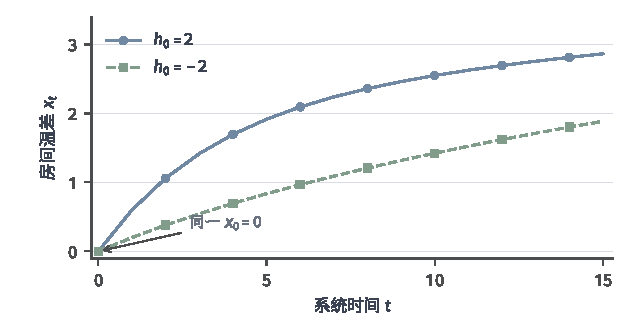
\includegraphics[width=107mm]{figures/00-shared/mathematical-preliminaries-lower/02-dynamical-systems-control-decision-and-games/matplotlib/reader-state-sufficiency/figure.pdf}
  \caption{室温单坐标遗漏墙体蓄热时的预测差异。按正文给出的无噪声双状态教学模型逐步计算，两条曲线的房间初始温差均为$x_0=0$，恒定加热量均为$0.4$；仅墙体初始温差$h_0$分别取$2$与$-2$。相同当前室温对应不同后继轨迹，说明应按未来依赖选择状态。}
  \label{fig:reader-state-sufficiency}
\end{figure}


初始条件规定轨迹从哪里开始，输入规定沿途施加什么作用，演化规律规定这些作用
怎样改变状态。输出则是模型对外显示的量。无噪声且传感器直接测温时可以有
$y_t=x_t$，但一般输出只给状态的部分信息。后文恢复过程噪声与观测噪声时，
仍使用同一时序：时刻$t$的状态已经形成，传感器产生$y_t$，然后给定的$u_t$
把状态推向$t+1$。只有在控制问题中，才进一步规定如何依据这些信息选择$u_t$。

图~\ref{fig:temperature-model-physical-objects}将温度例中的物理对象与模型变量对应起来：房间温差是状态，加热作用是给定输入，传感器读数是输出。

\begin{figure*}[htbp]
  \centering
  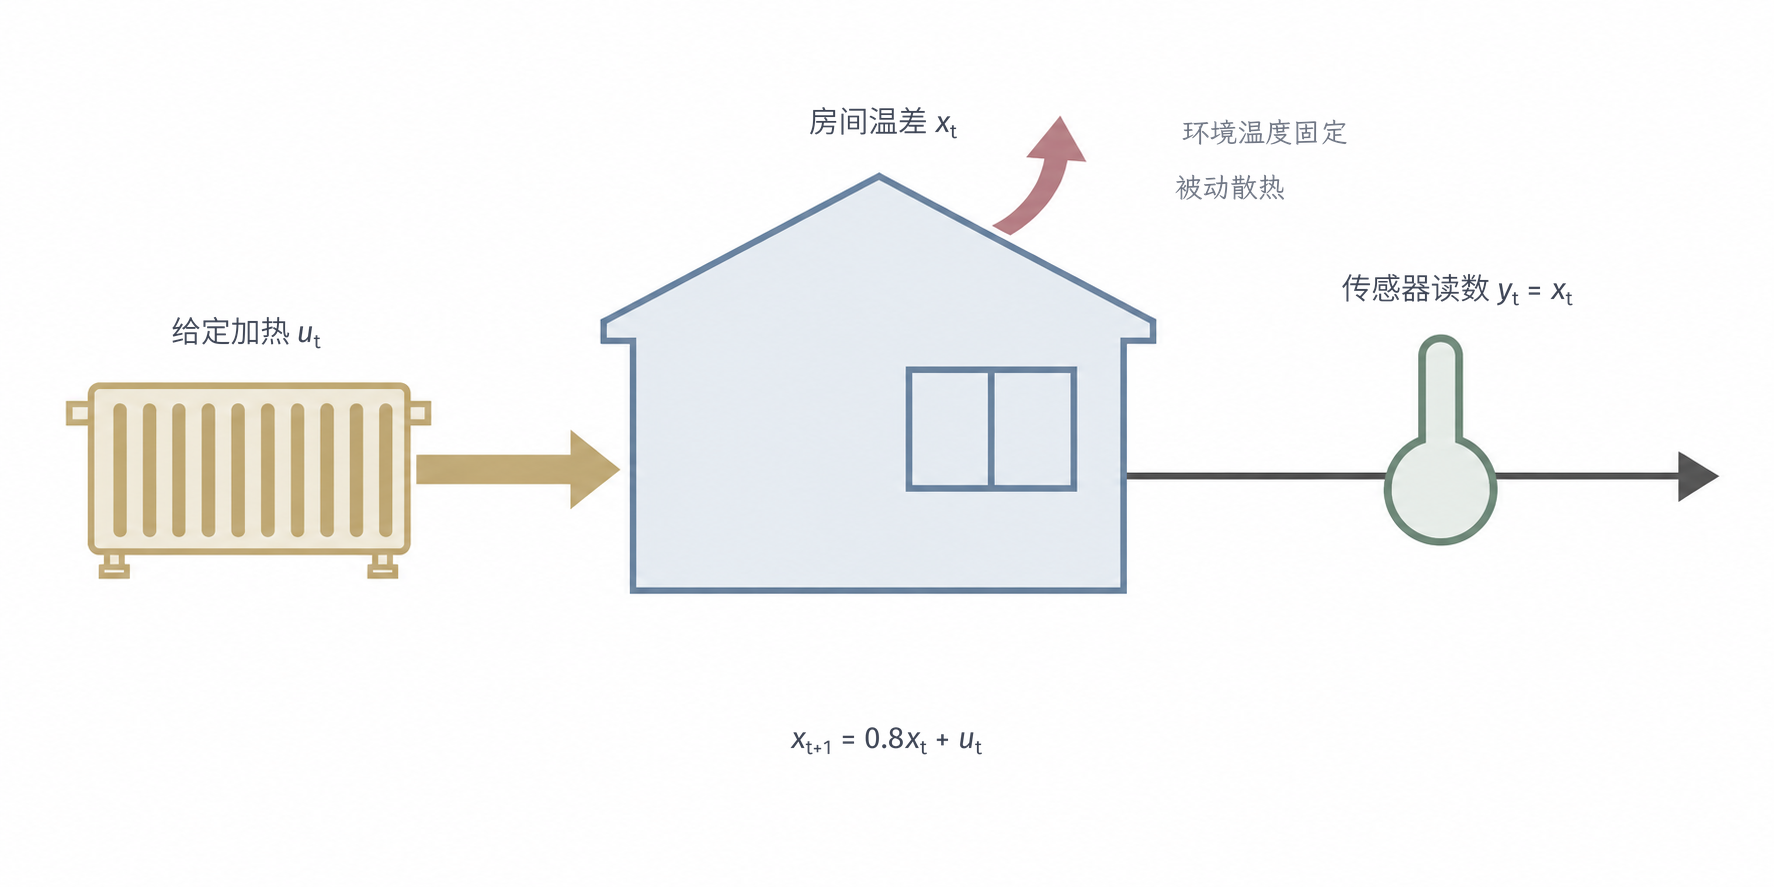
\includegraphics[width=\linewidth]{figures/00-shared/mathematical-preliminaries-lower/02-dynamical-systems-control-decision-and-games/generated/temperature-state-observation/figure.png}
  \caption{温度模型中的状态、输入与输出。环境温度固定时，$x_t$表示房间相对环境的温差，
  $u_t$表示给定加热输入，传感器在时刻$t$读取$y_t=x_t$。
  随后按$x_{t+1}=0.8x_t+u_t$形成下一时刻温差；系数$0.8$表示未加热时保留下来的温差比例。
  向外散热箭头示意房间温度高于环境时的传热；图中没有根据读数选择输入的控制器。}
  \label{fig:temperature-model-physical-objects}
\end{figure*}

\subsection{离散时间下的状态更新}
设$\mathcal X$是允许的状态集合，$\mathcal U$是输入集合。一步更新映射
\[
  F_t:\mathcal X\times\mathcal U\longrightarrow\mathcal X,\qquad
  \bm x_{t+1}=F_t(\bm x_t,\bm u_t)
\]
直接规定下一状态。只要初值属于$\mathcal X$、每个输入属于$\mathcal U$，且映射
确实把状态送回$\mathcal X$，有限步递推便有定义。若只在某个区域内给出公式，
则每一步还要检查结果是否留在该区域。本文温度例暂不加输入或状态约束。

线性模型常写为
\[
  \bm x_{t+1}=\bm A_t\bm x_t+\bm B_t\bm u_t,\qquad
  \bm x_t\in\mathbb R^d,\quad \bm u_t\in\mathbb R^m.
\]
它关于状态与输入的联合变量是线性的；固定非零输入后，它关于状态通常是仿射的。
矩阵不随$t$改变称为时不变，显式随$t$改变则称为时变。是否线性与是否时变是两项
独立性质。若$\bm A_t$还依赖当前状态或输入，虽然公式仍有“矩阵乘状态”的外形，
整体映射通常已不是线性的。

一个可直接计算的模型是带泄漏的记忆：
\begin{equation}
  x_{t+1}=a x_t+b u_t,\qquad x_0\ \text{给定}.
  \label{eq:dynamical-leaky-discrete-memory}
\end{equation}
温度例对应$a=0.8,b=1$。系数$a$控制已有信息保留多少，$b$控制新输入进入多少。
能逐步计算并不说明长期状态有界；同一公式取$|a|>1$便可能放大早期扰动。

\subsection{连续时间下的状态变化}
若关注相邻采样时刻之间发生了什么，需要规定瞬时变化率，而不仅是相隔一步的差值。离散递推只告诉你“每隔一分钟温度变成多少”，却没有描述这一分钟之内连续发生的过程；要刻画任意时刻的变化，就要给出状态对时间的导数。
常微分方程（ordinary differential equation, ODE）初值问题写为
\begin{equation}
  \dot{\bm x}(t)=\bm f(t,\bm x(t),\bm u(t)),\qquad
  \bm x(t_0)=\bm x_0.
  \label{eq:dynamical-general-ivp}
\end{equation}
给定输入后，右侧是作用在当前状态上的向量场。若它不显含时间，称方程为自治的；
否则为非自治的。恒定矩阵配上随时间变化的外部输入，也会产生非自治方程。
向量场告诉我们“现在往哪里、以多快速度移动”，有限时间转移还要由积分确定。

为比较离散更新与连续变化，令采样时刻为$t_n=n\Delta t$，
用$\widehat x_n$近似连续状态$x(t_n)$。若在每个间隔内把变化率冻结为左端的值，
并把泄漏记忆的系数取为$a=1-\lambda\Delta t$、$b=\Delta t$，则
\[
  \frac{\widehat x_{n+1}-\widehat x_n}{\Delta t}
    =-\lambda\widehat x_n+u(t_n).
\]
这一步更新称为前向Euler近似：用当前变化率乘以间隔长度，估计这一段的状态变化。
若步长趋零时相应极限成立，对应的连续模型为
\begin{equation}
  \dot x(t)=-\lambda x(t)+u(t).
  \label{eq:dynamical-leaky-continuous-memory}
\end{equation}
这里建立的是一种近似规则。它与连续解有多接近，可以在固定物理时刻比较。
取\(\lambda=0.2\)、恒定输入\(u(t)=0.4\)及\(\Delta t=1\)，
则\(a=0.8,b=1\)。连续方程的平衡点是\(u/\lambda=2\)，
与离散式的\(b u/(1-a)=2\)相同，说明两边描述的是同一个平衡位置。
一步衰减因子也接近：\(e^{-0.2}\approx0.819\)对\(0.8\)。
从相同初值\(x(0)=\widehat x_0=0\)出发，连续解为\(x(t)=2(1-e^{-0.2t})\)，
在\(t=5\)处给出\(1.264\)，而离散递推的\(\widehat x_5\)为\(1.345\)，
相差约\(0.08\)；到\(t=20\)时差距缩到\(0.014\)。
差别来自离散化把区间内的指数衰减替换成了一次线性衰减，
因此该例中的离散偏差比连续偏差衰减得快，最终两者仍趋于同一平衡。
若把步长减半为\(\Delta t=0.5\)，对应的\(a=1-\lambda\Delta t=0.9\)，
输入系数也须改为\(b=0.5\)。此时到达同一物理时刻\(t=5\)需要递推\(10\)步，
所得\(\widehat x_{10}\approx1.303\)，误差约为\(0.038\)；
到\(t=20\)需要\(40\)步，误差约为\(0.007\)。这些数字说明，
在固定有限时域上缩小步长，会减小这种Euler近似的误差；本例的误差按步长一阶缩小。

精确采样使用另一种更新关系。若\(\lambda>0\)，且每个采样间隔内的输入固定为\(u\)，
将平衡偏差记为\(z=x-u/\lambda\)，则\(\dot z=-\lambda z\)，所以
\[
  x(t+\Delta t)-\frac u\lambda
    =e^{-\lambda\Delta t}\left(x(t)-\frac u\lambda\right).
\]
移项得到
\[
  x(t+\Delta t)=e^{-\lambda\Delta t}x(t)
      +\frac{1-e^{-\lambda\Delta t}}{\lambda}u.
\]
因此精确采样的系数为\(a=e^{-\lambda\Delta t}\)、
\(b=(1-e^{-\lambda\Delta t})/\lambda\)。在输入按区间保持不变的条件下，
这项等式对任意正步长都成立；小步长决定Euler近似是否接近它。
例如\(e^{-\lambda\Delta t}=1-\lambda\Delta t+O(\Delta t^2)\)，
输入系数也等于\(\Delta t+O(\Delta t^2)\)，于是可恢复前面的线性近似。

反过来，贯穿例中的一步系数$0.8$是已给定的离散模型参数，
仅凭这个数不能唯一反推出连续模型。采用Euler参数化时要求
\(1-\lambda\Delta t=0.8\)，采用精确采样时要求
\(e^{-\lambda\Delta t}=0.8\)；在步长尚未约定时，两种规则各自都容许多组参数。
即使确定了步长和衰减率，还要按所采用的规则核对输入系数\(b\)及输入的单位，
才能判断整个离散更新是否对应同一个连续系统。

并非所有系统都耗散已有状态。位置相同但速度不同的运动会有不同未来，因此力学中
常把位置和动量合在一起作为状态；这个状态所在的空间称为相空间。
例如一个粒子的质量为\(m>0\)，位置为\(q\)、动量为\(p\)，势能为可微函数\(U(q)\)。它的方程为\(\dot q=p/m\)、\(\dot p=-U'(q)\)。位置变化由动量决定，动量变化由势能坡度决定；把势能与动能相加为\(H=U(q)+p^2/(2m)\)，位置更新恰好是对\(p\)求偏导，动量更新是对\(q\)求偏导后取负号。这给出用一个能量函数组织成对状态方程的方式。
\begin{definition}[可分Hamilton系统]
  \label{def:dynamical-separable-hamiltonian-system}
  令$\bm q,\bm p\in\mathbb R^d$分别为位置与动量，$U$为连续可微的势能，
  $\bm M$为对称正定的质量矩阵。可分Hamilton量为
  \begin{equation}
    H(\bm q,\bm p)=U(\bm q)+\frac12\bm p^\top\bm M^{-1}\bm p.
    \label{eq:dynamical-separable-hamiltonian}
  \end{equation}
  相应的Hamilton方程为
  \begin{equation}
    \dot{\bm q}=\nabla_{\bm p}H,\qquad
    \dot{\bm p}=-\nabla_{\bm q}H.
    \label{eq:dynamical-hamilton-equations}
  \end{equation}
\end{definition}
第一式由动量得到位置速度，第二式由势能坡度得到动量变化。令
$\bm z=(\bm q^\top,\bm p^\top)^\top$，则方程也可写为
\[
  \dot{\bm z}=\bm J\nabla H(\bm z),\qquad
  \bm J=\begin{bmatrix}\bm0&\bm I\\-\bm I&\bm0\end{bmatrix}.
\]
它不是沿$-\nabla H$下降，而是把梯度转换为成对坐标之间的运动方向。
例如$U(q)=q^2/2,M=1$给出$\dot q=p,\dot p=-q$，位置与动量轮流交换。
轨迹是否唯一、能量是否保持、怎样数值推进，将分别在相应条件下证明。

图~\ref{fig:reader-hamilton-gradient-flow}在同一个能量函数上比较这两种运动方向。取$H(q,p)=(q^2+p^2)/2$，Hamilton向量场为$(p,-q)$，与梯度$(q,p)$正交，所以
\[
  \frac{\mathrm dH}{\mathrm dt}=qp+p(-q)=0.
\]
若改用负梯度向量场$(-q,-p)$，则同样的链式计算给出
$\mathrm dH/\mathrm dt=-q^2-p^2$。前者沿等能量圆周运动，后者向原点下降；能量函数相同，演化规律仍可完全不同。

\begin{figure}[htbp]
  \centering
  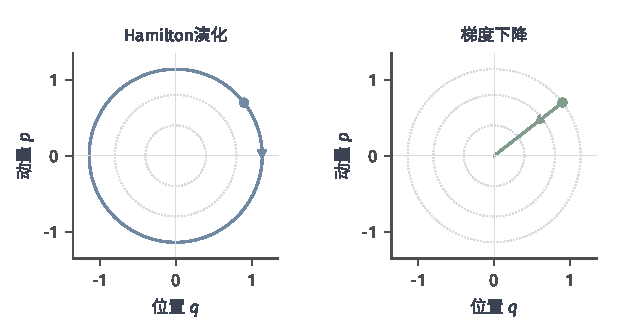
\includegraphics[width=107mm]{figures/00-shared/mathematical-preliminaries-lower/02-dynamical-systems-control-decision-and-games/matplotlib/reader-hamilton-gradient-flow/figure.pdf}
  \caption{同一函数$H(q,p)=(q^2+p^2)/2$下的两类精确轨迹。两面板均从$(q_0,p_0)=(0.9,0.7)$出发，绘制$0\leq t\leq2\pi$；灰色虚线是相同的能量等值线，箭头表示运动方向。左侧Hamilton系统$\dot q=p,\dot p=-q$保持能量，右侧负梯度系统$\dot q=-q,\dot p=-p$使能量下降。}
  \label{fig:reader-hamilton-gradient-flow}
\end{figure}


\subsection{随机扰动下的状态演化}
\label{sec:dynamical-ito-fokker-planck}

给定相同初温与加热量，开门、风速等未显式建模的作用仍可能改变真实温度。
把这些作用表示成过程噪声后，更新公式不再只产生一条确定轨迹，而是把噪声的联合
规律转换为状态的联合规律。本节只研究这种生成机制，尚未用任何传感器读数条件化。
离散更新可以直接逐步随机生成；连续时间必须先说明随机增量怎样累计。

\subsubsection{离散时间下的随机状态更新}
在同一概率空间上给定初始状态、输入及背景随机量，写
\[
  \bm x_{t+1}=F_t(\bm x_t,\bm u_t,\bm\varepsilon_{t+1}).
\]
若$\bm\varepsilon_{t+1}$独立于已有状态历史，分布为$\nu_{t+1}$，且$F_t$可测，
并将本节的输入$(\bm u_t)$固定为预先给定的确定序列，则由更新映射得到转移核
\[
  K_t(\bm x,A)=\int
    \mathbb I\{F_t(\bm x,\bm u_t,\bm e)\in A\}\,\nu_{t+1}(\mathrm d\bm e).
\]
对每个$\bm x$它是概率分布，对每个可测$A$它关于$\bm x$可测，因而是一个概率核：给每个当前状态指定一个下一步分布，且事件概率随状态可测地变化。独立性使
$\mathbb P(\bm x_{t+1}\in A\mid\bm x_{0:t})=K_t(\bm x_t,A)$，
这才得到当前状态的Markov性质。给定$\pi_0=\mathcal L(\bm x_0)$，整条有限轨迹满足
\[
  \mathbb P(\bm x_{0:T}\in\mathrm d\bm z_{0:T})
  =\pi_0(\mathrm d\bm z_0)
    \prod_{t=0}^{T-1}K_t(\bm z_t,\mathrm d\bm z_{t+1}),
\]
其中乘积表示逐次核积分。它同时规定跨时刻依赖，而不只是各个时刻的边缘分布。
若以后改用仅依赖当前状态的可测反馈$\bm u_t=\pi_t(\bm x_t)$，
把$\pi_t(\bm x)$代入核即可。若输入还依赖更早的状态或带噪观测，
仅有新噪声独立通常不足以使$\bm x_t$本身为Markov状态；
须保留相应历史或扩充状态。这一区别将在
\BookChapterRef{chap:control-theory}{第~\ref{chap:control-theory}章}“策略的实现与轨迹控制”中用于规定可实施策略。

常用的线性加性模型为
\begin{equation}
  \bm x_{t+1}=\bm A_t\bm x_t+\bm B_t\bm u_t+\bm w_{t+1}.
  \label{eq:dynamical-linear-state-model}
\end{equation}
若$\bm w_{t+1}\sim\mathcal N(\bm0,\bm Q_{t+1})$且独立于初态与其他过程噪声，
$K_t(\bm x,\cdot)=\mathcal N(\bm A_t\bm x+\bm B_t\bm u_t,\bm Q_{t+1})$。
即便$\bm Q_{t+1}$奇异，它仍是合法概率核，只是不一定有全维Lebesgue密度。

相关噪声需要重新检查条件结构。例如
$x_{t+1}=a x_t+w_{t+1}$，而$w_{t+1}=\rho w_t+\varepsilon_{t+1}$，
其中新$\varepsilon$独立。代入$w_t=x_t-a x_{t-1}$得
$x_{t+1}=(a+\rho)x_t-\rho a x_{t-1}+\varepsilon_{t+1}$。
一般仅给$x_t$已不足够；可把$(x_t,w_t)$扩成状态，或保留对更长历史的条件依赖。
“递推里有噪声”不等于“当前状态是Markov的”。

温度模型现在恢复为
\[
  x_{t+1}=0.8x_t+u_t+w_{t+1},\qquad
  w_{t+1}\sim\mathcal N(0,0.04).
\]
取各$w_t$相互独立且独立于初态。若$x_0=0,u_t=0.4$，
则$\mathbb E x_t=2(1-0.8^t)$，过程方差为
$0.04\sum_{j=0}^{t-1}0.8^{2j}$。平均轨迹仍与无噪模型相同，一条实际轨迹却会
在其附近波动。图~\ref{fig:action-state-temperature-layers}再叠加
$y_t=x_t+v_t$、$v_t\sim\mathcal N(0,0.09)$的独立读数噪声，
先展示生成层次；怎样由读数推断状态留到观测部分。

\begin{figure*}[htbp]
  \centering
  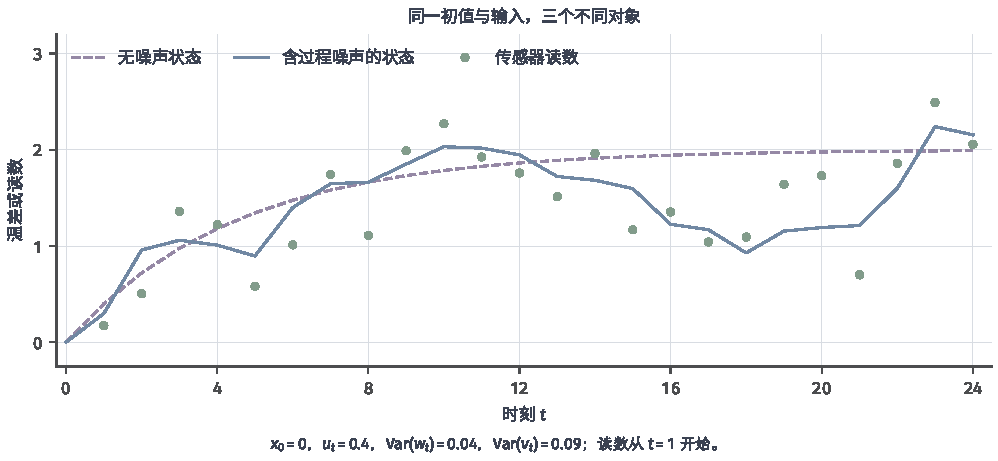
\includegraphics[width=\linewidth]{figures/00-shared/mathematical-preliminaries-lower/02-dynamical-systems-control-decision-and-games/matplotlib/action-state-temperature-layers/figure.pdf}
  \caption{同一温度模型的三个对象。初态$x_0=0$，输入始终为$0.4$；
  无噪声轨迹趋于$2$，过程噪声改变真实状态，独立观测噪声又把真实状态变成带噪读数。
  噪声方差分别为$0.04$和$0.09$。图中带噪曲线是固定种子的教学模拟，
  不是置信区间，也没有把读数用于反向校正状态。}
  \label{fig:action-state-temperature-layers}
\end{figure*}

\subsubsection{连续时间下的随机状态变化}
离散噪声可以逐次相加——每个采样间隔里有一个独立的随机扰动，直接加到下一状态上即可。连续时间却没有“最小的一步”：噪声在任意小的时间段里都在持续作用，必须先想清楚无穷多个无穷小的随机增量该如何累加。关键是按增量的方差尺度选择驱动。Brownian增量在长度\(h\)的区间上具有\(h\)阶方差（标准差为\(\sqrt h\)），Poisson驱动记录区间内到达的事件数。两类驱动可以改变同一个状态，但产生的路径不同：前者给连续而通常不可微的路径，后者允许状态在事件时刻突变。

给定漂移规律、噪声幅度与初值，建模任务是规定这些增量如何进入状态。第~\ref{sec:action-state-random-integrals}节将定义累计规则；建立规则后，第~\ref{sec:action-state-random-trajectory-solve}节才把状态相关系数写成完整的积分方程并讨论解。连续时间并不把驱动强行解释成普通时间导数。

\subsection{历史依赖下的状态表示}
前面从“一个能概括过去的状态”出发建模；现在换一个方向，从“我们想保留历史的哪些特征”出发构造状态。这种思路常见于用少量数字概括一段长信号的场合：例如不必逐点记住过去一小时的输入曲线，只保留它的平均值和线性趋势，就足以支持某些预测或控制。把输入投影到这几个特征函数张成的子空间上，所得的投影坐标就可以当作状态。
另一种构造从希望保留的历史特征出发。例如为一段输入保留平均值与线性趋势，
就可把投影坐标当作状态。固定$t>0$，取非负可测权重$w_t$，并以
$\mu_t(\mathrm ds)=w_t(s)\,\mathrm ds$规定$[0,t]$上的测度。要求输入$u$和所用基函数属于$L^2(\mu_t)$，函数按$\mu_t$几乎处处相等视为同一个元素。在这个空间上，随$t$改变的内积为
\[
  \langle f,g\rangle_t=\int_0^t f(s)g(s)w_t(s)\,\mathrm ds,
\]
并在一个$d$维子空间中选基$\phi_1^{(t)},\ldots,\phi_d^{(t)}$。线性无关性是对上述函数等价类而言；不能仅凭函数表达式不同就断言它们成基。若基正交归一，
$c_i(t)=\langle u,\phi_i^{(t)}\rangle_t$就是展开系数；一般基则要先构造
$G_{i,j}(t)=\langle\phi_i^{(t)},\phi_j^{(t)}\rangle_t$，
再由$\bm G(t)\bm a(t)=\bm c(t)$得到投影坐标$\bm a(t)$。
对任意非零向量$\bm b$，有
$\bm b^\top\bm G(t)\bm b=\|\sum_i b_i\phi_i^{(t)}\|_{L^2(\mu_t)}^2>0$，所以Gram矩阵可逆。
分析坐标$\bm c$和投影坐标$\bm a$不能在非正交基下混用；$t=0$时积分区间退化，初始状态须另行规定。

窗口本身移动时，状态变化不全来自新输入。固定宽度$T>0$，写
\[
  c_\ell(t)=\int_{t-T}^t u(s)\phi_\ell(t,s)w(t,s)\,\mathrm ds.
\]
在被积函数及所需偏导连续等Leibniz求导条件下，
\begin{align}
  \dot c_\ell(t)
  ={}&u(t)\phi_\ell(t,t)w(t,t)
    -u(t-T)\phi_\ell(t,t-T)w(t,t-T)\notag\\
  &+\int_{t-T}^t u(s)\partial_t[\phi_\ell(t,s)w(t,s)]\,\mathrm ds.
  \label{eq:dynamical-moving-window-coefficient}
\end{align}
这三项分别来自右端新输入、左端旧输入退出，以及窗口内部基或权重的改变。
漏掉左端项，就把固定长度窗口误当成只增长不遗忘的历史。

取均匀权重下的常数与一次矩，
\[
  c_0(t)=\frac1T\int_{t-T}^t u(s)\,\mathrm ds,\qquad
  c_1(t)=\frac2{T^2}\int_{t-T}^t(s-t+T)u(s)\,\mathrm ds,
\]
上式给出
\[
  \dot c_0(t)=\frac{u(t)-u(t-T)}T,\qquad
  \dot c_1(t)=\frac2T u(t)-\frac2T c_0(t).
\]
第二式在当前坐标与当前输入之间闭合，第一式仍需要窗口左端的值。
所以有限个历史特征不自动形成能独立接续演化的有限维状态；需要额外状态、特别的
基与权重，或对边界项作近似。

高阶多项式投影（high-order polynomial projection operators, HiPPO）框架
把历史投影到多项式空间，并以随时间更新的投影系数作为状态坐标\scite{gu2020hippo}
它保存哪些历史特征，由窗口、权重和基
共同决定。投影理论给出相应度量下的逼近误差，不意味着一般历史被无损保存，
也不自动保证所构造递推对扰动稳定。表示误差、演化闭合与稳定性要分别核对。

\section{路径的累计运算与状态变换}
\label{sec:action-state-path-operations}
\label{sec:action-state-random-integrals}
给定一段输入或随机增量，累计运算把它们沿时间的作用合在一起；对累计结果应用一个状态函数，则需要相应的变化公式。确定性输入的和与积分、跳跃增量的事件求和及Brownian增量的均方极限分别有不同的定义。只有先明确这些运算，才能把未知状态写进被积系数并求解轨迹。

\subsection{历史输入的累计作用}
\label{sec:signal-analysis-state-history-kernels}

先保持离散时间。对时不变系统，允许输出还直接依赖当前输入：
\begin{align}
  \bm x_{t+1}&=\bm A\bm x_t+\bm B\bm u_t,\notag\\
  \bm y_t&=\bm C\bm x_t+\bm D\bm u_t.
  \label{eq:signal-analysis-lti-state-space}
\end{align}
这里$\bm A\in\mathbb R^{d\times d}$、$\bm B\in\mathbb R^{d\times m}$、
$\bm C\in\mathbb R^{p\times d}$、$\bm D\in\mathbb R^{p\times m}$。
本章统一用$\bm x$表示状态、$\bm u$表示输入；信号表示中的输入记号不能在这里
继续兼作状态。直接项$\bm D\bm u_t$是本小节允许的一般输出通道，贯穿温度
传感器模型则取$\bm D=\bm0$，不改变“先读数、后输入推动下一状态”的时序。

前两步为$\bm x_1=\bm A\bm x_0+\bm B\bm u_0$及
$\bm x_2=\bm A^2\bm x_0+\bm A\bm B\bm u_0+\bm B\bm u_1$。归纳得到
\begin{equation}
  \bm x_t=\bm A^t\bm x_0+
    \sum_{\tau=0}^{t-1}\bm A^{t-1-\tau}\bm B\bm u_\tau.
  \label{eq:signal-analysis-state-unrolling}
\end{equation}
归纳步把右侧乘$\bm A$并加$\bm B\bm u_t$，求和上界与各项幂次就同时前移一格。
代入输出方程，
\begin{equation}
  \bm y_t=\bm C\bm A^t\bm x_0+\bm D\bm u_t+
    \sum_{\tau=0}^{t-1}\bm C\bm A^{t-1-\tau}\bm B\bm u_\tau.
  \label{eq:signal-analysis-state-convolution}
\end{equation}
第一项是初态的自由响应，其余项是输入响应。零初态时，定义
\begin{equation}
  \bm K_0=\bm D,\qquad
  \bm K_r=\bm C\bm A^{r-1}\bm B\quad(r\geq1),
  \label{eq:signal-analysis-state-kernel}
\end{equation}
就得到因果卷积$\bm y_t=\sum_{\tau=0}^t\bm K_{t-\tau}\bm u_\tau$。
核$\bm K_r$记录$r$步以前的输入经过剩余状态传播后对当前输出的作用。
非零初态的自由响应必须另加，不能塞进一个与输入无关的零状态卷积公式。

用标量$a=1/2,b=c=1,d=0,x_0=0$核对。依次输入
$u_0=1,u_1=2,u_2=1$，递推给出
$y_0=0,y_1=1,y_2=5/2,y_3=9/4$。核为
$K_0=0,K_1=1,K_2=1/2,K_3=1/4$，所以
\[
  y_3=K_3u_0+K_2u_1+K_1u_2=\frac14+1+1=\frac94.
\]
严格因果的状态通道使$y_0=0$；若$d\neq0$，当前输入还会立即通过$K_0=d$进入
输出。标量核$ca^{r-1}b$在$|a|<1$时几何衰减，在$|a|>1$时增长；多维状态
还需检查不同方向的传播，不能由核的形式本身断言稳定。

时变系统用有序乘积
\[
  \bm\Phi(t,s)=\bm A_{t-1}\cdots\bm A_s\quad(t>s),\qquad
  \bm\Phi(s,s)=\bm I
\]
传播齐次状态，于是
\[
  \bm x_t=\bm\Phi(t,0)\bm x_0+
    \sum_{\tau=0}^{t-1}\bm\Phi(t,\tau+1)\bm B_\tau\bm u_\tau.
\]
若输出为$\bm C_t\bm x_t+\bm D_t\bm u_t$，对应核为
\[
  \bm K_{t,t}=\bm D_t,\qquad
  \bm K_{t,\tau}=\bm C_t\bm\Phi(t,\tau+1)\bm B_\tau\quad(\tau<t).
\]
它依赖两个绝对时刻，通常不只依赖滞后$t-\tau$，所以线性仍在，平移不变性却已
消失。较晚矩阵必须置于左边。若这些矩阵还依赖输入或状态，展开系数也随输入轨迹
改变，叠加通常失效；固定轨迹附近的线性化核仅有局部含义。


\subsection{跳跃路径上的随机积分}
\label{sec:action-state-poisson-integral}

把更新间隔缩到连续时间后，“把每一步的随机增量加起来”这件事必须格外小心，因为积分同时遍历时间和随机结果两个维度。下面先解释为什么需要两个新条件。
离散更新只需说明每一步使用哪些已知量。把更新间隔缩到连续时间后，还须说明
被积系数在时间与随机结果的联合空间中是否可测。以下滤过
$(\mathcal F_t)_{t\geq0}$满足通常条件：$\mathcal F_0$包含概率零集的全部子集，
且$\mathcal F_t=\bigcap_{s>t}\mathcal F_s$。过程、滤过和停时的基础回见
第~\ref{chap:stochastic-processes-and-approximation}章。

每个时刻分别可测，还不足以保证沿时间积分有定义：积分同时遍历时间和随机结果。另一个限制来自事件先后次序，跳跃幅度不能由同一次尚未发生的跳跃决定。因此下面分别补充联合可测性与事前可用性；它们解决的是两个不同的要求。
一个过程$H$适应，表示每个$H_t$对$\mathcal F_t$可测。若对每个$T$，
$(t,\omega)\mapsto H_t(\omega)$在$[0,T]\times\Omega$上对
$\mathcal B([0,T])\otimes\mathcal F_T$可测，则称它渐进可测。
可预测过程则对由全部左连续适应过程生成的可预测$\sigma$代数可测。
这两项都包含时间方向的联合可测要求；逐时刻适应本身不够。
连续适应过程可预测；若$X$适应且路径右连续、有左极限，
则$X_{t-}$可预测，而跳跃后的$X_t$一般不能作为当次跳跃前已知的系数。

连续时间中也可以根据已经观察到的信息决定何时停止。
连续时间中的停时是取值于$[0,\infty]$的随机变量$\tau$，满足
$\{\tau\leq t\}\in\mathcal F_t$对每个实数$t\geq0$成立；
停止过程$M^\tau_t=M_{t\wedge\tau}$在到达$\tau$后保持当时的值。
若适应且右连续、有左极限的过程$M$存在递增停时$\rho_n\to\infty$几乎必然，
使每个$M^{\rho_n}$都是真鞅，就称$M$为局部鞅（local martingale）。
这里的“局部”是由随机停止限定的范围：每条路径最终能覆盖任意给定的有限时段，
却未保证去掉停止后仍能交换期望与极限。用这样的停止过程先证明结论、再逐步放开停止范围，称为局部化（localization）。

普通漂移的累计仍是逐路径的Lebesgue积分$\int_0^t b_s\,\mathrm ds$，
要求相应联合可测性及$\int_0^T|b_s|\,\mathrm ds<\infty$几乎必然。
噪声的累计规则则取决于增量类型：有限次跳跃可以逐事件相加，连续Brownian噪声
不能这样处理，也不能当作普通可积的时间导数。

令$N_t$为速率$\lambda>0$的Poisson计数过程，相对于共同滤过，
$N_t-N_s$独立于$\mathcal F_s$且服从$\operatorname{Pois}(\lambda(t-s))$。
记跳时为$\tau_1,\tau_2,\ldots$。有限活动指每个有界时间区间内几乎必然只有
有限个事件；它不要求整个无穷时间轴上事件总数有限。
对有限实值的可预测过程$H$，定义
\begin{equation}
  \int_0^t H_s\,\mathrm dN_s
    =\sum_{\tau_j\leq t}H_{\tau_j}.
  \label{eq:action-state-poisson-integral}
\end{equation}
若$H_s=g(s,X_{s-})$，第$j$个事件的贡献为$g(\tau_j,X_{\tau_j-})$。
事件已经发生后才知道的状态，不能反过来决定同一事件的可预测幅度。
上述和逐路径有定义；若还要交换期望与求和，需增加可积性。

对非负可预测$H$，Poisson补偿恒等式为
\[
  \mathbb E\int_0^T H_s\,\mathrm dN_s
       =\lambda\mathbb E\int_0^T H_s\,\mathrm ds.
\]
对简单过程$H_s=\sum_iH_i\mathbb I_{(t_i,t_{i+1}]}(s)$，
$H_i$对$\mathcal F_{t_i}$可测，等式由
$\mathbb E[H_i\Delta N_i]=\lambda\Delta t_i\mathbb E H_i$逐项相加得到。
从这些阶梯过程推广到一般可预测过程，还需核对可预测$\sigma$代数。
在$(0,T]\times\Omega$上，它由矩形$(a,b]\times A$生成，其中
$0\leq a<b\leq T$、$A\in\mathcal F_a$。
这一表示与前面左连续适应过程的定义一致：矩形的指示过程左连续且适应，
而左连续适应过程可用取左端点值的确定网格阶梯过程逐点逼近。
对可预测集合$B$定义两个有限测度
\[
 \mu_N(B)=\mathbb E\int_0^T\mathbb I_B(s,\omega)\,\mathrm dN_s,
 \qquad
 \mu_\lambda(B)=\lambda\mathbb E\int_0^T\mathbb I_B(s,\omega)\,\mathrm ds.
\]
两者在上述矩形上相等，且总质量均为$\lambda T$。
矩形族封闭于有限交，由单调类定理得到的测度唯一性因而把等式扩展到全部可预测集合。
再对非负可预测$H$使用一般简单函数逼近与Tonelli定理，便得到补偿恒等式，
允许两侧同时为无穷；这里不要求用确定网格阶梯过程单调逼近任意$H$。
正负部均可积时，分别应用该等式再相减，得到有符号版本。
因此$\lambda\mathbb E\int_0^T|H_s|\,\mathrm ds<\infty$保证跳跃和可积。

原计数同时包含平均增长与随机起伏。扣除平均增长，得到补偿计数
$\widetilde N_t=N_t-\lambda t$及积分
\begin{equation}
  \int_0^t H_s\,\mathrm d\widetilde N_s
    =\sum_{\tau_j\leq t}H_{\tau_j}
      -\lambda\int_0^t H_s\,\mathrm ds.
  \label{eq:action-state-compensated-poisson}
\end{equation}
若$\lambda\mathbb E\int_0^T H_s^2\,\mathrm ds<\infty$，
该过程为平方可积鞅，并满足
\begin{equation}
  \mathbb E\left|\int_0^T H_s\,\mathrm d\widetilde N_s\right|^2
       =\lambda\mathbb E\int_0^T H_s^2\,\mathrm ds.
  \label{eq:action-state-poisson-isometry}
\end{equation}
为核对这点，先取上述简单过程。每个$\Delta\widetilde N_i$在
$\mathcal F_{t_i}$条件下均值为零、方差为$\lambda\Delta t_i$。
对$i<j$，先在$\mathcal F_{t_j}$条件下求期望，便使
$H_i\Delta\widetilde N_iH_j\Delta\widetilde N_j$的期望为零。
平方展开只剩$\sum_i\lambda\Delta t_i\mathbb E H_i^2$。
同样的条件期望计算给出任意$s<t$间的鞅等式。
简单过程的二阶逼近、上述等距和条件期望的$L^2$连续性完成延拓；
补偿恒等式保证延拓与有限跳跃和表示一致。
若每个有限$T$上只有$\int_0^T H_s^2\,\mathrm ds<\infty$几乎必然，
可取
\[
 \rho_n=\inf\left\{t:\lambda\int_0^tH_s^2\,\mathrm ds\geq n\right\}\wedge n.
\]
累计平方是连续适应的非减过程，所以首次达到阈值可由当前历史判断，$\rho_n$为停时。
停止后的累计量不超过$n$，已证等距便保证相应补偿积分为平方可积鞅。
各有界区间的累计量有限又使$\rho_n\uparrow\infty$几乎必然，因此未停止的积分是局部鞅。
去掉停止时，逐路径收敛并不自动保留期望；还需例如固定时刻上停止变量族的一致可积性，才能据此得到零均值。

左极限不是无关紧要的记号。例如单位幅度事件有
\[
  \int_0^t N_{s-}\,\mathrm dN_s=\frac{N_t(N_t-1)}2,\qquad
  \sum_{\tau_j\leq t}N_{\tau_j}=\frac{N_t(N_t+1)}2.
\]
右侧第二个和使用了事件后的计数，两者相差$N_t$。
若错误地把$N_s$当作可预测系数，则
\[
  \mathbb E\left[\sum_{\tau_j\leq t}N_{\tau_j}
       -\lambda\int_0^t N_s\,\mathrm ds\right]=\lambda t\neq0.
\]
它不是声称的零均值补偿积分。用$N_{s-}$时，多出来的这一项恰好消失。

\subsection{连续路径上的随机积分}
以下$\bm W$是在同一滤过下的$m$维标准Brownian运动，分量独立，
其增量独立于过去且协方差为时间长度乘$\bm I_m$。定义、路径性质以及
$[W^{(i)},W^{(j)}]_t=\delta_{i,j}t$回见
第~\ref{sec:dynamical-brownian-motion}节；本处只构造如何累计这些增量。
这里要构造的是关于Brownian积分器的\(\int H_t\,\mathrm dW_t\)，而不是把Brownian路径当作普通被积函数的\(\int W_t\,\mathrm dt\)。后一积分因\(W\)连续而可逐路径定义。前一积分则要累加\(H\)加权的Brownian增量；Brownian路径在每个非退化紧时间区间上几乎必然具有无限总变差，不能直接把它当作通常有界变差的Stieltjes积分器来处理一般随机被积过程。某些特殊被积函数仍可逐路径积分，例如光滑确定性\(H\)可用分部积分；这里需要的是适用于更一般适应平方可积过程的统一构造。Brownian独立增量的方差等于时间长度，因而可先对简单过程定义加权增量和，再用均方误差关系延拓。
先用标量驱动，把可预测简单过程写为
$H_t=\sum_{i=0}^{n-1}H_i\mathbb I_{(t_i,t_{i+1}]}(t)$，
其中$0=t_0<\cdots<t_n=T$，$H_i\in L^2(\mathcal F_{t_i})$。
定义
\begin{equation}
  \int_0^T H_t\,\mathrm dW_t
       :=\sum_{i=0}^{n-1}H_i(W_{t_{i+1}}-W_{t_i}).
  \label{eq:dynamical-simple-ito-integral}
\end{equation}
系数可以依赖已发生的全部历史，但不能借用下一段增量。

记
$M_t=\sum_iH_i(W_{t\wedge t_{i+1}}-W_{t\wedge t_i})$。
对$s<t$，包含$s$的区间使用已知系数和$s$之后的零均值增量；
对起点$t_i\geq s$的后续区间，塔式性质给出
\[
  \mathbb E[H_i\Delta W_i\mid\mathcal F_s]
   =\mathbb E\{\mathbb E[H_i\Delta W_i\mid\mathcal F_{t_i}]
                  \mid\mathcal F_s\}=0.
\]
截断到$t$的最后一段同理。因此$\mathbb E[M_t\mid\mathcal F_s]=M_s$，
$M$是平方可积鞅，特别地$\mathbb E M_T=0$。
再核对平方：对$i<j$，$H_iH_j\Delta W_i$对$\mathcal F_{t_j}$可测，
故
\[
  \mathbb E[H_iH_j\Delta W_i\Delta W_j]=0,\qquad
  \mathbb E[H_i^2(\Delta W_i)^2]=\Delta t_i\,\mathbb E H_i^2.
\]
无界系数时可先截断再用$L^2$极限；交叉乘积由Cauchy--Schwarz保证可积。
逐项相加得到\term{Itô等距}：
\begin{equation}
  \mathbb E\left(\int_0^T H_t\,\mathrm dW_t\right)^2
       =\mathbb E\int_0^T H_t^2\,\mathrm dt.
  \label{eq:dynamical-ito-isometry}
\end{equation}
这与Poisson等距的推导结构相同，但此处尚没有逐路径的有限事件和。

对可预测$H$，若$\mathbb E\int_0^T H_t^2\,\mathrm dt<\infty$，
用简单可预测过程在该范数下逼近，等距关系使积分序列在$L^2$中为Cauchy序列，
从而定义与逼近选择无关的积分。条件期望是$L^2$压缩映射，故鞅性质保留；
所得鞅可取连续版本。渐进可测且平方可积的系数可在
$\mathbb P\otimes\mathrm dt$意义下取等价可预测版本，得到同一积分。
若每个有限$T$上只有$\int_0^T H_t^2\,\mathrm dt<\infty$几乎必然，则取
\[
 \rho_n=\inf\left\{t:\int_0^tH_s^2\,\mathrm ds\geq n\right\}\wedge n.
\]
这与Poisson积分的停止构造相同，只是不再乘速率$\lambda$。
停止后平方积分至多为$n$，所以可用Itô等距构造真鞅；
这些积分在共同的停止区间上一致，随$\rho_n\uparrow\infty$拼接成连续局部鞅。
矩阵系数逐分量积分时，等距右端改为Frobenius范数平方。

普通积分与Brownian积分的路径粗糙程度不同。路径$A$在$[0,T]$上有限变差
（finite variation），是指全部分割$\pi$上的绝对增量和有共同有限上界：
\[
 \operatorname{Var}_{[0,T]}(A)
 =\sup_\pi\sum_i|A_{t_{i+1}}-A_{t_i}|<\infty.
\]
这里求和的是绝对增量；二次变差则累计增量的平方，两者不是同一性质。
对$A_t=\int_0^t b_s\,\mathrm ds$，三角不等式给出
$\operatorname{Var}_{[0,T]}(A)\leq\int_0^T|b_s|\,\mathrm ds$，
因此漂移累计具有有限变差。向量情形可逐分量使用同一判断。
把漂移与Brownian累计合起来，就得到后面换元公式的对象。
\begin{definition}[连续Itô过程]
  \label{def:action-state-ito-process}
  设$\bm X_0$对$\mathcal F_0$可测，$\bm b_t$渐进可测，
  $\bm\sigma_t$可预测，且每个有限$T$上
  $\int_0^T(\|\bm b_t\|+\|\bm\sigma_t\|_{\mathrm F}^2)\,\mathrm dt<\infty$
  几乎必然。过程
  \[
    \bm X_t=\bm X_0+\int_0^t\bm b_s\,\mathrm ds
                         +\int_0^t\bm\sigma_s\,\mathrm d\bm W_s
  \]
  称为连续Itô过程。漂移积分有有限变差，随机积分是连续局部鞅。
\end{definition}
这里系数已经给定；若系数反过来依赖未知的$\bm X_t$，才形成待求解的方程。

积分约定可以由Brownian平方直接辨认：
\[
 W_{t_{i+1}}^2-W_{t_i}^2
     =2W_{t_i}\Delta W_i+(\Delta W_i)^2.
\]
求和并回用二次变差，左端点和趋于$(W_T^2-T)/2$，右端点和趋于
$(W_T^2+T)/2$。两者差$T$，不是随着网格变细就消失的误差。
左端点与右端点累计已经给出不同答案。如果改为对称地使用两端系数，就需要记录这两种取样差产生的交叉增量修正。为统一表达漂移与连续随机波动，下面先把对象扩大为有限变差部分与连续局部鞅之和，再用二次协变差表示修正；Stratonovich约定将在这一范围内恢复普通链式法则。
连续半鞅是可分解为连续局部鞅与连续适应有限变差过程之和的过程；
前述Itô过程属于这一类。其二次协变差$[H,X]_t$由分割上
$\sum_i\Delta H_i\Delta X_i$的概率极限定义。
若$A$有限变差且$X$连续，交叉增量和满足
\[
 \left|\sum_i\Delta A_i\Delta X_i\right|
 \leq\max_i|\Delta X_i|\operatorname{Var}_{[0,T]}(A)
 \longrightarrow0.
\]
最后一步来自连续路径在紧区间上一致连续。因此这类因子与连续随机项的二次协变差为零，稍后线性方程的积分因子将使用这个性质。
对于连续半鞅$H,X$，
Stratonovich积分可定义为
\[
  \int_0^t H_s\circ\mathrm dX_s
       =\int_0^t H_s\,\mathrm dX_s+\tfrac12[H,X]_t.
\]
对本章的Itô过程，右侧积分按漂移与Brownian部分分别计算；
一般半鞅积分使用相应延拓。该定义对应对称端点和的概率极限。
在系数足够光滑的标量模型中，
$\mathrm dX=b_{\mathrm S}(X)\,\mathrm dt+\sigma(X)\circ\mathrm dW$
等价于Itô漂移$b_{\mathrm I}=b_{\mathrm S}+\sigma\sigma'/2$。
多维时修正为$\frac12\sum_j(D\bm\sigma_{\cdot j})\bm\sigma_{\cdot j}$。
Stratonovich形式保留普通链式法则，但不能只更换积分符号而不改漂移。
上述规则限定连续半鞅；跳跃换元要另外保留有限差。

\subsection{连续随机演化下的状态函数变换}
读数、能量和损失通常是状态的函数，因此需要计算它们沿随机轨迹怎样变化。对有限变差的连续轨迹，分割增量的平方和趋于零，普通链式法则不留下二阶累计项。单位Brownian驱动\(W\)不同：在固定时段\([0,t]\)上，确定性分割的网格趋零时，\(\sum_i(\Delta W_i)^2\)依概率趋于\(t\)。一般Itô状态\(\bm X\)的第\(i,j\)个坐标之间的二次协变差还要保留扩散系数：
\[
 [X^i,X^j]_t
 =\int_0^t(\bm\sigma_s\bm\sigma_s^\top)_{ij}\,\mathrm ds.
\]
例如\(X=2W\)的二次变差是\(4t\)，不是\(t\)。这些不消失的二次累计项与状态函数的二阶导数结合，才产生Itô公式中的修正；不能把所有连续随机状态的平方增量和都认作经过的时间。

可以用等分网格直接比较这两个累计尺度。将$[0,1]$分为$n$段，记
$Q_n^W=\sum_{i=0}^{n-1}(W_{(i+1)/n}-W_{i/n})^2$。
每个增量独立且服从$\mathcal N(0,1/n)$，正态四阶矩给出
\[
  \mathbb E Q_n^W=1,\qquad
  \mathbb E(Q_n^W-1)^2=\frac2n.
\]
因此平方和本身保留在$1$附近，缩小的是它与$1$的均方偏差。相比之下，光滑路径$a(t)=t$的每段增量恰为$1/n$，平方和为$n(1/n)^2=1/n$，直接趋于零。图~\ref{fig:reader-quadratic-variation-scale}画出这些精确量；Brownian项留下二阶修正的原因是平方增量的累计不消失，而非连续路径都具有同一变化规律。

\begin{figure}[htbp]
  \centering
  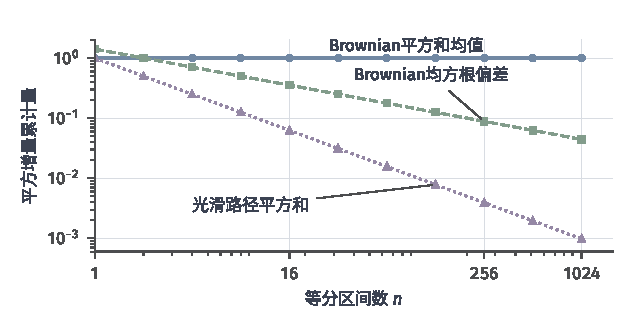
\includegraphics[width=107mm]{figures/00-shared/mathematical-preliminaries-lower/02-dynamical-systems-control-decision-and-games/matplotlib/reader-quadratic-variation-scale/figure.pdf}
  \caption{等分$[0,1]$时平方增量的累计尺度，双轴均为对数刻度。蓝线为单位Brownian运动平方和的精确均值$\mathbb E Q_n^W=1$，绿虚线为均方根偏差$\{\mathbb E(Q_n^W-1)^2\}^{1/2}=\sqrt{2/n}$，紫点线为光滑路径$a(t)=t$的平方和$1/n$。图中画的是解析矩与确定性累计量，没有模拟随机路径，绿线也不是置信区间。}
  \label{fig:reader-quadratic-variation-scale}
\end{figure}

一次跳跃又不能视为无穷小位移，跳跃处要用完整的有限差值。这两种情形分别需要二阶修正与完整有限差。


\begin{theorem}[Itô公式]
  \label{thm:dynamical-ito-formula}
  设$\bm X$为定义~\ref{def:action-state-ito-process}中的过程，
  $f\in C^{1,2}([0,T]\times\mathbb R^d)$，即时间一阶、空间二阶偏导连续。
  则存在同一个概率零集，使下式在该零集之外对所有$t\in[0,T]$同时成立。
  其微分记号为
  \begin{align}
    \mathrm df(t,\bm X_t)
      &=[\partial_t f+\nabla f^\top\bm b_t
         +\tfrac12\operatorname{tr}
               (\bm\sigma_t\bm\sigma_t^\top\nabla^2 f)]\,\mathrm dt\notag\\
      &\quad+\nabla f^\top\bm\sigma_t\,\mathrm d\bm W_t.
    \label{eq:dynamical-ito-formula}
  \end{align}
  各导数在$(t,\bm X_t)$取值。若要对等式直接取期望，还须漂移项可积，
  且随机被积项满足例如
  $\mathbb E\int_0^T\|\nabla f^\top\bm\sigma_t\|^2\,\mathrm dt<\infty$；
  局部鞅本身不保证期望为零。
\end{theorem}

先说明关键估计，以免把二阶项当作形式记忆规则。对有界连续适应系数，
局部化后的Taylor展开中，漂移平方和的期望为$O(|\pi|)$，
漂移与随机项乘积和的$L^1$范数为$O(|\pi|^{1/2})$；
这里$|\pi|$为分割的最大间距。这些项均消失。相反，对有界的
$\mathcal F_{t_i}$可测权重$c_i$，独立增量与正态四阶矩给出
\[
 \mathbb E\left|\sum_i c_i[(\Delta W_i)^2-\Delta t_i]\right|^2
   =2\sum_i\mathbb E[c_i^2](\Delta t_i)^2
   \leq2\sup_i\|c_i\|_\infty^2T|\pi|.
\]
不同Brownian分量的交叉乘积也以同样方式趋零。故加权平方项留下
时间积分，而不是零；矩阵写法恰为
$\operatorname{tr}(\bm\sigma\bm\sigma^\top\nabla^2f)/2$。

把$\Delta\bm X_i$中的系数冻结在左端点，也要控制误差。连续有界系数满足
\[
 \mathbb E\sum_i
 \left\|\int_{t_i}^{t_{i+1}}
    (\bm\sigma_s-\bm\sigma_{t_i})\,\mathrm d\bm W_s\right\|^2
 =\mathbb E\int_0^T
       \|\bm\sigma_s-\bm\sigma_{\lfloor s\rfloor_\pi}\|_{\mathrm F}^2\,\mathrm ds
 \longrightarrow0.
\]
漂移差用普通积分估计；一阶随机项用Itô等距控制。
在紧区域内，Hessian一致连续，空间Taylor余项的绝对值和至多为
$\omega(\max_i\|\Delta\bm X_i\|)\sum_i\|\Delta\bm X_i\|^2$，
其中$\omega(r)\to0$。路径连续使第一个因子趋零，第二个因子依上述估计
在概率上有界；余项因而依概率趋零。时间一阶项由$\partial_t f$的一致连续性处理。
这解释了光滑且系数连续有界时每类项的去向。

一般可测系数不能擅自用左端取样逼近。完整结果先按状态大小及累计可积量停时，
再以简单可预测过程逼近随机系数，并用连续局部鞅的二次协变差处理上述加权项，
最后令停时递增。这一一般化及$C^{1,2}$版本的完整证明见
Øksendal的随机微分方程教材第4章；上面的关键估计说明机制，不替代该一般证明\scite{math-oksendal2003sde}

例如$f(x)=x^2$给出
\[
  W_T^2=2\int_0^T W_s\,\mathrm dW_s+T,\qquad
  \int_0^T W_s\,\mathrm dW_s=(W_T^2-T)/2.
\]
常数系数则有$\int_0^T c\,\mathrm dW_s=cW_T$。
形式规则$(\mathrm dW)^2=\mathrm dt$、$\mathrm dt\,\mathrm dW=0$
总结了上述累计量级；它们不能替代可预测性与极限论证。

\subsection{跳跃随机演化下的状态函数变换}
\label{sec:action-state-jump-ito}

考虑连续Itô部分加有限活动跳跃的右连续过程
\[
  \bm X_t=\bm X_0+\int_0^t\bm b_s\,\mathrm ds
        +\int_0^t\bm\sigma_s\,\mathrm d\bm W_s
        +\int_0^t\bm\gamma_s\,\mathrm dN_s,
\]
其中$\bm\gamma$可预测、在各事件处有限，$\bm b,\bm\sigma$满足前述局部
可积条件。对同样的$f\in C^{1,2}$，换元公式为
\begin{align}
 f(t,\bm X_t)-f(0,\bm X_0)
  ={}&\int_0^t[\partial_s f+\nabla f^\top\bm b_s
       +\tfrac12\operatorname{tr}(\bm\sigma_s\bm\sigma_s^\top\nabla^2f)]
                           (s,\bm X_{s-})\,\mathrm ds\notag\\
   &+\int_0^t\nabla f(s,\bm X_{s-})^\top\bm\sigma_s\,\mathrm d\bm W_s\notag\\
   &+\int_0^t[f(s,\bm X_{s-}+\bm\gamma_s)-f(s,\bm X_{s-})]\,\mathrm dN_s.
 \label{eq:action-state-jump-ito}
\end{align}
第一行中$\bm b_s,\bm\sigma_s$是过程系数，只把$f$的导数在所示点取值。
当跳跃次数与状态先被停时截断后，在相邻事件之间应用连续Itô公式，
到事件$\tau_j$处再加上精确增量
$f(\tau_j,\bm X_{\tau_j})-f(\tau_j,\bm X_{\tau_j-})$。
有限次相加，端点望远镜消去，即得此式。再去除截断，因有限活动与局部可积性，
得到每个有限时域上的结论。这一推导不需要把跳幅假设为很小。

若把$\nabla f^\top\mathrm d\bm X$统一写在前面，则还须显式加上
\[
 \sum_{\tau_j\leq t}
 [f(\tau_j,\bm X_{\tau_j})-f(\tau_j,\bm X_{\tau_j-})
          -\nabla f(\tau_j,\bm X_{\tau_j-})^\top\Delta\bm X_{\tau_j}].
\]
它不是只有二阶的近似，而是扣掉已计入一阶项后的全部有限差。
对补偿形式
$\mathrm d\bm X=\bm\beta_s\,\mathrm ds+\bm\sigma_s\,\mathrm d\bm W
                      +\bm\gamma_s\,\mathrm d\widetilde N$，
记$\Delta_\gamma f=f(s,\bm X_{s-}+\bm\gamma_s)-f(s,\bm X_{s-})$，
则$f$的漂移为
\[
 \partial_s f+\nabla f^\top\bm\beta_s
 +\tfrac12\operatorname{tr}(\bm\sigma_s\bm\sigma_s^\top\nabla^2f)
 +\lambda(\Delta_\gamma f-\nabla f^\top\bm\gamma_s),
\]
跳跃鞅项为$\Delta_\gamma f\,\mathrm d\widetilde N_s$。
由$\bm b=\bm\beta-\lambda\bm\gamma$及
$\mathrm dN=\mathrm d\widetilde N+\lambda\,\mathrm ds$代入即可核对；
取期望仍须检查该新被积项的可积性。

令$X=N$、$f(x)=x^2$，每次事件使平方增加$2N_{s-}+1$，所以
\[
  N_t^2=\int_0^t(2N_{s-}+1)\,\mathrm dN_s
       =2\int_0^tN_{s-}\,\mathrm d\widetilde N_s
         +\widetilde N_t+2\lambda\int_0^tN_s\,\mathrm ds+\lambda t.
\]
于是$\mathbb E N_t^2=(\lambda t)^2+\lambda t$。
Brownian平方的修正为连续的$t$，Poisson平方的修正为事件计数$N_t$；
后者再补偿才分成鞅与平均漂移。把两者都写成“噪声平方等于时间”会丢失事件信息。

\section{状态轨迹与分布的求解}
\label{sec:action-state-trajectory-computation}
给定初值、输入和演化规律后，所求结果可以是一条确定轨迹，也可以是噪声驱动的一条随机轨迹，或某时刻的状态分布。精确方程有解只建立求解对象；不能解析求解时，还要用离散计算近似它。下面把这些查询分开，避免将观测后的推断与无观测的演化求解混用。

\subsection{离散时间下的初值轨迹求解}


\subsubsection{基于逐步递推的轨迹求解}
把给定输入吸收进$F_t^{\bm u}(\bm x)=F_t(\bm x,\bm u_t)$，前两步为
\[
  \bm x_1=F_0^{\bm u}(\bm x_0),\qquad
  \bm x_2=F_1^{\bm u}\bigl(F_0^{\bm u}(\bm x_0)\bigr).
\]
一般状态是有序复合
$\bm x_t=(F_{t-1}^{\bm u}\circ\cdots\circ F_0^{\bm u})(\bm x_0)$。
较晚更新写在左边，因为它作用于较早更新的结果；调换复合顺序会改变系统。

泄漏模型可进一步展开：
\begin{equation}
  x_t=a^t x_0+\sum_{j=0}^{t-1}a^{t-1-j}b u_j.
  \label{eq:dynamical-discrete-variation-constants}
\end{equation}
证明从$t=0$的空和开始。若式子对$t$成立，两边乘$a$再加$b u_t$，
便得到$t+1$的式子。初值与每次输入的贡献都在其中：旧输入经历的更新次数更多，
因而多乘若干个$a$。

取独立于温度任务的泄漏例$a=1/2,b=1,x_0=0$。仅在第零步输入$u_0=1$时，
$x_1=1,x_2=1/2,x_3=1/4$；若$u_0=u_1=1$，则$x_2=3/2$，
其中$1/2$来自旧输入，$1$来自新输入。这就是状态保存的历史总作用。
回到温度例，$u_t=0.4$给出
\[
  x_t=2+0.8^t(x_0-2).
\]
有限步展开已经得到轨迹；它趋于$2$还使用了$|0.8|<1$。一般非线性映射可逐步计算，
却未必有这样的闭式或极限。

\paragraph{指数递归平均的记忆与方差}
\label{sec:dynamical-exponential-average}
若输入是同一量的连续观测，希望用一个状态平滑短时波动，可以把泄漏更新取为
\begin{equation}
 M_n=(1-\alpha)M_{n-1}+\alpha Y_n,\qquad n\geq1,\quad 0<\alpha\leq1.
 \label{eq:dynamical-exponential-average}
\end{equation}
这里$Y_n$是第$n$次输入，$M_n$是吸收该输入后的状态。这称为\term{指数移动平均}
（exponential moving average, EMA）。令$a=1-\alpha$，由前面的仿射展开得到
\begin{equation}
 M_n=a^nM_0+\alpha\sum_{j=1}^n a^{n-j}Y_j.
 \label{eq:dynamical-exponential-average-expansion}
\end{equation}
初值与历次输入的权重之和为$1$，但有限步内仅观测项的权重之和为$1-a^n$。
若$M_0=0$只表示尚无观测，除以$1-a^n$可把这些观测权重重新归一化；
若$M_0$本来就是有效的初始估计，这样做会改变原先指定的更新。
对$0<\alpha<1$，一项旧输入经过$k$步后保留比例$a^k$，
降至$\mathrm e^{-1}$所需的实数步数为$-1/\log(1-\alpha)$，小$\alpha$时约为$1/\alpha$。
$\alpha=1$时只保留当前输入。

平滑能减少多少噪声，需要另加观测条件。设$Y_n=\mu+\varepsilon_n$，
各$\varepsilon_n$相互独立、均值为零、方差为$\sigma^2$，
$M_0\in L^2$并独立于全部观测噪声。初始偏差满足
$\mathbb E M_n-\mu=a^n(\mathbb E M_0-\mu)$。
记$v_n=\operatorname{Var}(M_n)$；$M_{n-1}$只依赖初值与过去噪声，
故与$\varepsilon_n$独立，方差递推及其解为
\begin{equation}
 \begin{aligned}
 v_n&=a^2v_{n-1}+\alpha^2\sigma^2\\
    &=a^{2n}v_0+\frac{\alpha}{2-\alpha}
                        (1-a^{2n})\sigma^2
      \longrightarrow\frac{\alpha}{2-\alpha}\sigma^2.
 \end{aligned}
 \label{eq:dynamical-exponential-average-variance}
\end{equation}

例如$\alpha=0.2$时极限方差为$\sigma^2/9$，这一数值以真值不变和独立噪声为前提。
较小的$\alpha$同时延长旧输入的残留时间。若观测改为$Y_n=\mu_n+\varepsilon_n$，
真值每步增加$d$，即$\mu_n=\mu_0+nd$，令$b_n=\mathbb E M_n-\mu_n$，则
$b_n=a b_{n-1}-ad$，长期偏差为$-ad/\alpha$。
所以降低常值观测下的方差，也会增加跟随持续变化时的滞后；
相关噪声还会在方差递推中增加协方差项。

采样间隔变化时，固定$\alpha$把记忆长度固定在步数上，不能固定在物理时间上。
给定时间尺度$\tau>0$，在每段长度$\Delta t_n>0$的区间把输入保持为$y_n$，
精确积分$\tau\dot m=y_n-m$，得到
\[
 M_n=\mathrm e^{-\Delta t_n/\tau}M_{n-1}
       +(1-\mathrm e^{-\Delta t_n/\tau})y_n.
\]
因此可取$\alpha_n=1-\mathrm e^{-\Delta t_n/\tau}$。
它给出相同物理时间尺度下的指数遗忘，精确性仍以每段内输入保持不变为条件；
固定权重下的方差极限也不能直接用于这组变化的权重。

\subsubsection{基于并行扫描的仿射轨迹求解}
逐步递推沿时间形成一条严格的串行依赖链：算\(x_2\)必须先有\(x_1\)，算\(x_3\)又必须先有\(x_2\)，无法并行。但如果每一步都是仿射映射，就有一个加速的机会：任意连续若干步仿射更新复合后仍然是一个同样大小的仿射映射（仿射映射复合仍为仿射映射），于是可以先把相邻的更新两两合并、再把合并结果继续合并，自底向上压成一棵二叉树，从而并行求出所有中间状态。并行扫描改变的只是求值的括号和执行安排，所计算的更新规则保持不变。考虑仿射递推
\begin{equation}
  \bm x_{t+1}=\bm A_t\bm x_t+\bm b_t,
  \label{eq:dynamical-affine-recurrence}
\end{equation}
用二元组$g_t=(\bm A_t,\bm b_t)$表示一步，定义较晚更新接在较早更新之后的复合为
\begin{equation}
  (\bm A_2,\bm b_2)\circ(\bm A_1,\bm b_1)
  =(\bm A_2\bm A_1,\bm A_2\bm b_1+\bm b_2).
  \label{eq:dynamical-affine-composition}
\end{equation}
复合结果仍是同维度仿射映射，这是能够紧凑表示整段更新的关键。三步直接核对得
\[
  \begin{aligned}
    g_3\circ(g_2\circ g_1)
    &=(\bm A_3\bm A_2\bm A_1,\,
       \bm A_3\bm A_2\bm b_1+\bm A_3\bm b_2+\bm b_3)\\
    &=(g_3\circ g_2)\circ g_1.
  \end{aligned}
\]
结合律允许用前缀扫描（prefix scan）同时求全部$g_{t-1}\circ\cdots\circ g_0$。
把更新按时间次序放在一棵平衡二叉树的叶子上，上行阶段合并相邻块，
每个内部节点保存自己整段的总复合。这个阶段只得到块的总映射，
全部中间状态还需要一次下传。

下传时，节点接收其区间之前已经完成的累计映射$p$。
左孩子继续接收$p$；若左块的总映射是$L$，右孩子就接收$L\circ p$。
根节点接收恒等映射$(\bm I,\bm0)$。例如四步$g_0,g_1,g_2,g_3$时，
左半块的总映射为$L=g_1\circ g_0$，四个叶子接收到的前缀分别是
\[
 \begin{aligned}
 p_0&=\operatorname{id},&p_1&=g_0,\\
 p_2&=L,&p_3&=g_2\circ L.
 \end{aligned}
\]
叶子$i$再形成$g_i\circ p_i$并作用于$\bm x_0$，便得到$\bm x_{i+1}$。
右块始终接在左块之后，所以这套下传规则也适用于不交换的复合。

总工作量统计所有节点执行的合并次数，计算深度统计最长依赖链上的合并次数。
$T$步形成的平衡树有$O(T)$个节点、$O(\log T)$层，
上下两阶段在每个节点只做常数次合并，同层互不依赖的节点可同时计算。
因此把一次固定维度合并视为一个操作时，总工作量为$O(T)$，深度为$O(\log T)$。
矩阵维度增长时，合并的实际算术成本仍需另算。

扫描保留时间次序。若$g_1(\bm x)=\operatorname{diag}(2,1)\bm x$、
$g_2(\bm x)=\bm x+(1,0)^\top$，则
\[
  (g_2\circ g_1)(\bm0)=(1,0)^\top,\qquad
  (g_1\circ g_2)(\bm0)=(2,0)^\top.
\]
这两个结果说明结合律不能换成交换律。浮点运算下，改变括号也可能改变舍入结果，
尤其是长乘积或条件数较大的传播；并行实现应按误差容限验证，而不是要求逐位相同。
若$\bm A_t,\bm b_t$只依赖事先给定的输入，仍可预先组成仿射扫描；若依赖尚未
算出的状态，或复合后不再有固定大小的封闭表示，就需要另行分析，不能直接套用。

\subsection{连续时间下的初值轨迹求解}


\subsubsection{初值约束下的轨迹存在与延拓}
一个“几乎处处给出斜率”的公式，要能恢复整条曲线，必须排除没有被导数记录的
奇异变化。为什么要引入“绝对连续”这个看似技术性的条件？因为仅说一条曲线连续、并且几乎处处可导是不够的：存在连续（甚至严格递增）的函数，它几乎处处导数为零，却并不是常量——导数在极少数点之外都为零，可曲线的变化恰恰藏在那些点里，靠积分导数无法还原。为此采用绝对连续曲线，而非任意连续曲线。
连续性只排除跳跃，不能保证全部变化都能由导数积分恢复；因此仅在几乎处处规定斜率仍可能遗漏变化。这里要求“初值加一个可积速度的累计”恰好等于曲线本身，使微分方程与积分方程能够互相对应。这是对曲线的正则性要求，区别于前面比较两个测度零集的绝对连续。
\begin{definition}[绝对连续曲线]
  \label{def:dynamical-absolutely-continuous-curve}
  有限区间$[a,b]$上的曲线$\bm x:[a,b]\to\mathbb R^d$称为
  \term{绝对连续曲线}，若存在$\bm v\in L^1([a,b];\mathbb R^d)$，使
  $\bm x(t)=\bm x(a)+\int_a^t\bm v(s)\,\mathrm ds$对每个$t$成立。
  此时$\dot{\bm x}=\bm v$几乎处处成立。
\end{definition}
记$\bm g(t,\bm x)=\bm f(t,\bm x,\bm u(t))$。积分意义下的解就是满足
\begin{equation}
  \bm x(t)=\bm x_0+\int_{t_0}^t\bm g(s,\bm x(s))\,\mathrm ds
  \label{eq:dynamical-ivp-integral-form}
\end{equation}
的绝对连续曲线。当$\bm g$连续时，它还是处处满足微分方程的经典解。

\begin{theorem}[局部存在唯一性]
  \label{thm:dynamical-picard-lindelof}
  若给定输入后的$\bm g$在$(t_0,\bm x_0)$附近连续，且关于状态局部Lipschitz，
  Lipschitz常数可在该时间邻域内统一选取，则存在包含$t_0$的区间，使
  式~\eqref{eq:dynamical-general-ivp}有唯一局部解。
\end{theorem}
\begin{proof}
  在适用邻域内选闭区域
  \[
    D=[t_0-a,t_0+a]\times
    \{\bm x:\|\bm x-\bm x_0\|_2\leq b\}.
  \]
  紧性给出$M=\sup_D\|\bm g\|_2<\infty$；记统一Lipschitz常数为$L$。
  选$h>0$使$h\leq a,Mh\leq b,Lh<1$。在$I=[t_0-h,t_0+h]$上，
  \[
    \mathcal X=\{\bm z\in C(I,\mathbb R^d):
       \|\bm z-\bm x_0\|_\infty\leq b\}
  \]
  是完备空间的闭子集，因而完备。定义
  $(\mathcal T\bm z)(t)=\bm x_0+\int_{t_0}^t\bm g(s,\bm z(s))\,\mathrm ds$。
  对$\bm z\in\mathcal X$，
  $\|(\mathcal T\bm z)(t)-\bm x_0\|_2\leq M|t-t_0|\leq Mh\leq b$，
  所以$\mathcal T$映回$\mathcal X$。同时
  \[
    \|\mathcal T\bm z_1-\mathcal T\bm z_2\|_\infty
    \leq Lh\|\bm z_1-\bm z_2\|_\infty.
  \]
  压缩映射定理给出唯一不动点，即积分方程的解。任何同初值的局部解在足够短的
  区间内都落在$\mathcal X$，故与此解重合；在共同存在区间逐段重复便得到局部唯一性。
\end{proof}

这个证明把三种条件分开使用：连续性给出有界的局部变化率，完备性让迭代的极限仍是
候选曲线，统一Lipschitz条件使积分算子在短区间收缩。只有连续性不保证唯一性。
例如$\dot x=\sqrt{|x|},x(0)=0$既有零解，也有对任意$c\geq0$定义的
\[
  x(t)=
  \begin{cases}
    0,&0\leq t\leq c,\\
    (t-c)^2/4,&t>c.
  \end{cases}
\]
解可以任意等待后再离开原点。

局部解能通过重叠区间的唯一性接成长一些的解。不能再向外接续的解称为最大解；
最大区间包含全部所需时刻时，才得到相应的全局解。局部光滑仍可能有限时间爆炸：
$\dot x=x^2,x(0)=1$的解$x(t)=1/(1-t)$在$t=1$前已无界。
排除这种情况，需要增长控制。下面的估计也是后文比较两条轨迹的共同工具。

\begin{lemma}[Grönwall积分估计]
  \label{lem:action-state-gronwall}
  设$e$为$[a,T]$上非负连续函数，$b$为非负可积函数。若
  \[
    e(t)\leq c+\int_a^t b(s)e(s)\,\mathrm ds,\qquad c\geq0,
  \]
  则$e(t)\leq c\exp(\int_a^t b(s)\,\mathrm ds)$。
  更一般地，若右侧另有$\int_a^t r(s)\,\mathrm ds$，其中$r\geq0$可积，则
  \[
    e(t)\leq c\,\mathrm e^{\int_a^t b}
      +\int_a^t r(s)\,\mathrm e^{\int_s^t b}\,\mathrm ds.
  \]
\end{lemma}
\begin{proof}
  令$E(t)=c+\int_a^t[b(s)e(s)+r(s)]\,\mathrm ds$，则$e\leq E$，
  且$E'\leq bE+r$几乎处处成立。乘以绝对连续的积分因子
  $\exp(-\int_a^t b)$，使用乘积法则并从$a$积分到$t$，得
  \[
    E(t)\mathrm e^{-\int_a^t b}
    \leq c+\int_a^t r(s)\mathrm e^{-\int_a^s b}\,\mathrm ds.
  \]
  再乘回积分因子并用$e\leq E$即可；取$r=0$得到第一式。
\end{proof}

若$\|\bm g(t,\bm x)\|\leq b(t)\|\bm x\|+r(t)$，其中$b,r$在每个有限时间区间
可积，积分方程与此引理给出有限的状态上界。在局部存在条件持续有效、状态域为
$\mathbb R^d$时，这排除了有限时间逃逸，因而最大解可延拓到任意有限时刻。
全局Lipschitz以及$\|\bm g(t,\bm0)\|$的局部可积性是常用的充分条件。
对仅时间可测的输入还需相应的Carathéodory条件：$\bm g$关于时间可测、
关于状态连续，并在紧状态集上有可积上界与可积Lipschitz系数。不能把上述连续
输入版本的局部定理原样套给任意不可测输入。

\subsubsection{线性演化下的轨迹求解}
连续时间对应的时不变方程是
\begin{equation}
  \dot{\bm x}(t)=\bm A\bm x(t)+\bm B\bm u(t).
  \label{eq:dynamical-lti-continuous}
\end{equation}
对固定有限方阵$\bm A$，矩阵指数由级数
$\mathrm e^{t\bm A}=\sum_{j\geq0}t^j\bm A^j/j!$定义。由次乘性，第$j$项的范数
不超过$(|t|\lVert\bm A\rVert)^j/j!$，所以级数对每个$t$绝对收敛，逐项求导后的级数
在有界区间上一致收敛，于是
$\frac{\mathrm d}{\mathrm dt}\mathrm e^{t\bm A}
=\bm A\mathrm e^{t\bm A}=\mathrm e^{t\bm A}\bm A$；
$t\bm A$与$-t\bm A$可交换，两级数相乘后按总次数合并得
$\mathrm e^{t\bm A}\mathrm e^{-t\bm A}=\bm I$，即$\mathrm e^{t\bm A}$的逆为$\mathrm e^{-t\bm A}$。
用矩阵范数判断矩阵级数收敛的做法可参考\BookChapterRef{chap:linear-analysis}{卷1《数学准备：计算、分析与几何》的“谱和奇异值”章}。令
$\bm z(t)=\mathrm e^{-t\bm A}\bm x(t)$，乘积求导给出
$\dot{\bm z}(t)=\mathrm e^{-t\bm A}\bm B\bm u(t)$。积分并乘回指数，得到
\begin{equation}
  \bm x(t)=\mathrm e^{(t-t_0)\bm A}\bm x_0+
    \int_{t_0}^t\mathrm e^{(t-s)\bm A}\bm B\bm u(s)\,\mathrm ds.
  \label{eq:dynamical-lti-variation-constants}
\end{equation}
代入$t_0$得到初值；对积分上限求导得到原方程，因而这确实是解，而非只是一种
形式展开。局部可积输入给出积分意义的解，连续输入给出经典解。标量泄漏模型取
$\lambda>0,u(t)\equiv u_0$时，
\[
  x(t)=\mathrm e^{-\lambda(t-t_0)}x_0+
    \frac{1-\mathrm e^{-\lambda(t-t_0)}}{\lambda}u_0.
\]
初值作用消退，持续输入则留下$u_0/\lambda$，两种贡献不能一起称为“趋零”。

时变系数需要连续时间的传播算子。
\begin{definition}[状态转移矩阵]
  \label{def:dynamical-state-transition-matrix}
  对连续矩阵函数$\bm A(t)$，\term{状态转移矩阵}$\bm\Phi(t,s)$是满足
  \begin{equation}
    \partial_t\bm\Phi(t,s)=\bm A(t)\bm\Phi(t,s),\qquad
    \bm\Phi(s,s)=\bm I
    \label{eq:dynamical-state-transition-matrix}
  \end{equation}
  的矩阵值解。它把时刻$s$的齐次初态映到时刻$t$。
\end{definition}
由解的唯一性，$\bm\Phi(t,r)\bm\Phi(r,s)=\bm\Phi(t,s)$。
反向传播给出$\bm\Phi(t,s)^{-1}=\bm\Phi(s,t)$；用该逆矩阵作积分因子，得到
\begin{equation}
  \bm x(t)=\bm\Phi(t,t_0)\bm x_0+
    \int_{t_0}^t\bm\Phi(t,s)\bm B(s)\bm u(s)\,\mathrm ds.
  \label{eq:dynamical-ltv-variation-constants}
\end{equation}
对输出$\bm C(t)\bm x(t)+\bm D(t)\bm u(t)$，连续历史核是
$\bm C(t)\bm\Phi(t,s)\bm B(s)$，直接项仍单列。时不变时它退化为滞后核
$\bm C\mathrm e^{(t-s)\bm A}\bm B$。

一般不能令$\bm\Phi(t,s)=\exp(\int_s^t\bm A(r)\,\mathrm dr)$。
例如先运行常矩阵$\bm A_1$一单位时间，再运行$\bm A_2$一单位时间，实际传播为
$\mathrm e^{\bm A_2}\mathrm e^{\bm A_1}$；当两矩阵不交换时，一般不能将它
化为$\mathrm e^{\bm A_1+\bm A_2}$。若不同时间矩阵彼此交换，
则可把时序传播写成积分矩阵的指数；一般情形仍须保留传播次序。

\subsection{随机扰动下的初值轨迹求解}
\label{sec:action-state-random-trajectory-solve}
前面的随机积分累计给定系数；现在让系数随未知状态变化，便要寻找与累计结果相容的整条轨迹。给定初值和同一条噪声驱动后，轨迹能否被唯一确定？若只给初值分布而允许重新构造驱动，又能确定怎样的路径规律？下面先明确这两种求解要求，再给出存在与唯一条件。

\begin{definition}[Itô随机微分方程与强解]
  \label{def:dynamical-ito-sde-strong-solution}
  在给定的通常滤过概率空间上，设$\bm W$为$m$维Brownian运动，
  $\bm X_0$为$\mathcal F_0$可测初值。给定联合Borel可测系数
  $\bm b:[0,T]\times\mathbb R^d\to\mathbb R^d$、
  $\bm\sigma:[0,T]\times\mathbb R^d\to\mathbb R^{d\times m}$，
  Itô\term{随机微分方程}的扩散形式为
  \begin{equation}
    \mathrm d\bm X_t=\bm b(t,\bm X_t)\,\mathrm dt
                  +\bm\sigma(t,\bm X_t)\,\mathrm d\bm W_t.
    \label{eq:dynamical-ito-sde}
  \end{equation}
  解是满足局部可积条件的连续适应过程，使
  \[
    \bm X_t=\bm X_0+\int_0^t\bm b(s,\bm X_s)\,\mathrm ds
                  +\int_0^t\bm\sigma(s,\bm X_s)\,\mathrm d\bm W_s
  \]
  以概率$1$对所有$t$同时成立。若解适应于初值和给定驱动的历史所生成、
  完成并取右连续版本的滤过，则称为\term{强解}；它不另外使用随机信息。
\end{definition}

再给定速率$\lambda$的Poisson过程$N$，并规定$\bm W,N,\bm X_0$相互独立，
以其共同历史生成滤过；更一般的模型必须显式保证两类驱动在共同滤过下仍有
前述增量与补偿性质。有限活动跳跃扩展为
\begin{equation}
 \bm X_t=\bm X_0+\int_0^t\bm b(s,\bm X_{s-})\,\mathrm ds
      +\int_0^t\bm\sigma(s,\bm X_{s-})\,\mathrm d\bm W_s
      +\int_0^t\bm\gamma(s,\bm X_{s-})\,\mathrm dN_s.
 \label{eq:action-state-jump-sde}
\end{equation}
此时要求解右连续且有左极限。若采用补偿积分，须把漂移改为
$\bm b+\lambda\bm\gamma$才能表示同一个模型。
强解的定义相应包含$N$的历史。

例如
$\mathrm dX_t=-\lambda_0X_{t-}\,\mathrm dt+\sigma\,\mathrm dW_t
                         +c\,\mathrm dN_t$
描述连续泄漏、连续扰动以及每个事件带来的$c$单位突变，其中$\lambda_0>0$
为泄漏率，$\lambda$仍为事件速率。连续时间只是时间参数连续，
不意味着路径可微或没有跳跃。

弱解允许概率空间、驱动和过程一起作为待求对象，但它们必须满足同样的驱动联合
条件、初值分布及积分方程。路径唯一性比较同一空间、同一初值和同一驱动上的
两个解，要求它们不可区分，即几乎必然在所有时刻相同。
分布唯一性则只要求任意弱解的状态路径分布相同：扩散情形在连续路径空间上比较，
跳跃情形在右连续有左极限的路径空间上比较。
因此“弱”不是数值精度较低，“强”也不是稳定性更强。
给定噪声后能否逐路径确定状态，与只确定状态的概率规律，是不同要求。

\subsubsection{随机初值问题的存在与唯一性}
为证明状态相关的随机积分方程有解，可以反复将上一条候选轨迹代入被积系数。相邻候选的误差需要在整个有限时段上一同控制；Itô等距只给出固定终点的二阶误差，鞅最大不等式将它扩展到时段内的最大波动。
\begin{lemma}[二阶鞅最大不等式]
 \label{lem:action-state-doob-l2}
 若$\bm M$是右连续平方可积鞅，则
 \[
   \mathbb E\sup_{t\leq T}\|\bm M_t\|^2
      \leq4\mathbb E\|\bm M_T\|^2.
 \]
\end{lemma}
\begin{proof}
 $\|\bm M_t\|$由条件Jensen不等式为非负次鞅。记
 $S=\sup_{t\leq T}\|\bm M_t\|$。在有限网格首次越过$a$的时刻条件化，
 得
 \[
  a\mathbb P(S_{\rm grid}>a)
    \leq\mathbb E[\|\bm M_T\|\mathbb I_{\{S_{\rm grid}>a\}}].
 \]
 取越来越密且包含$T$的网格，由右连续性得到同样的$S$不等式。
 对$a\in[0,R]$积分并用尾积分公式，
 \[
  \mathbb E(S\wedge R)^2
    \leq2\mathbb E[\|\bm M_T\|(S\wedge R)]
    \leq2\|\bm M_T\|_{L^2}\|S\wedge R\|_{L^2}.
 \]
 若右端第二因子为零，则截断上确界几乎必然为零，左侧也为零；否则除去该因子再平方，令$R\uparrow\infty$即可。
\end{proof}

\begin{theorem}[SDE强解的存在唯一性]
 \label{thm:dynamical-sde-strong-existence}
 设$\bm W$在通常滤过下为标准Brownian运动，
 $\bm X_0\in L^2(\mathcal F_0)$。联合Borel可测的$\bm b,\bm\sigma$
 在$[0,T]$上满足统一全局Lipschitz与线性增长条件
 \begin{align*}
 \|\bm b(t,\bm x)-\bm b(t,\bm y)\|
 +\|\bm\sigma(t,\bm x)-\bm\sigma(t,\bm y)\|_{\mathrm F}
    &\leq L\|\bm x-\bm y\|,\\
 \|\bm b(t,\bm x)\|^2+\|\bm\sigma(t,\bm x)\|_{\mathrm F}^2
    &\leq C(1+\|\bm x\|^2).
 \end{align*}
 则式~\eqref{eq:dynamical-ito-sde}存在唯一强解，具有路径唯一性，且
 $\mathbb E\sup_{t\leq T}\|\bm X_t\|^2<\infty$。
\end{theorem}
\begin{proof}
 在短区间$[a,a+h]$固定平方可积初值$\bm\xi$，取连续适应过程的空间，
 范数为$\|\bm Z\|_{\mathcal S^2}^2
 =\mathbb E\sup_{a\leq t\leq a+h}\|\bm Z_t\|^2$，过程按不可区分等价。
 这是完备空间：Cauchy列可选子列几乎必然一致收敛，极限连续且适应，
 再用范数Cauchy性质得到$\mathcal S^2$收敛。
 定义
 \[
  (\mathcal T\bm Z)_t=\bm\xi+\int_a^t\bm b(s,\bm Z_s)\,\mathrm ds
                         +\int_a^t\bm\sigma(s,\bm Z_s)\,\mathrm d\bm W_s.
 \]
 Borel系数与连续适应过程的复合渐进可测；增长界、Cauchy--Schwarz、
 Itô等距和最大不等式使$\mathcal T$映回该空间。
 对两过程作差，同样的估计给出
 \[
 \begin{aligned}
 \|\mathcal T\bm Z-\mathcal T\bm Y\|_{\mathcal S^2}^2
 &\leq(2hL^2+8L^2)\int_a^{a+h}
                   \mathbb E\|\bm Z_s-\bm Y_s\|^2\,\mathrm ds\\
 &\leq2L^2h(h+4)\|\bm Z-\bm Y\|_{\mathcal S^2}^2.
 \end{aligned}
 \]
 取$h$使最后系数小于$1$，压缩映射定理给出唯一不动点。
 从常值过程开始的Picard迭代只用$\bm\xi$和驱动历史，极限为强解。
 用区间末状态作为下一段初值，在同样长度的有限多个区间上接续得到$[0,T]$解。

 为核对矩与无爆炸，记$S(t)=\mathbb E\sup_{r\leq t}\|\bm X_r\|^2$。
 三项平方界与前述估计给出
 \[
  S(t)\leq3\mathbb E\|\bm X_0\|^2
       +3C(T+4)\int_0^t[1+S(s)]\,\mathrm ds.
 \]
 引理~\ref{lem:action-state-gronwall}给出有限上界。
 对同初值同驱动的两个$\mathcal S^2$解，记
 \[
  D(t)=\mathbb E\sup_{r\leq t}\|\bm X_r-\bm Y_r\|^2.
 \]
 同样的估计给出
 \[
  D(t)\leq2L^2(T+4)\int_0^tD(s)\,\mathrm ds.
 \]
 再用该引理便有$D=0$。
 对一般连续局部解，先在两者离开半径$R$的球之前使用同一估计；
 再令$R\uparrow\infty$，由增长界及连续性去掉停时，得到路径唯一性。
\end{proof}

上述构造的每次迭代都是初值与驱动的同一个可测函数，极限的分布因此由它们的
联合分布确定，也给出这里的分布唯一性。只有局部Lipschitz时，截断系数先给出
离开任意有界区域前的解；线性增长或合适Lyapunov矩界还需用来排除爆炸。
光滑系数本身不够，零扩散下的$\dot X=X^2$已经是反例。

对式~\eqref{eq:action-state-jump-sde}，有限速率$N$在$[0,T]$上只有有限跳时。
在两次事件间解扩散方程，在$\tau_j$处设
$\bm X_{\tau_j}=\bm X_{\tau_j-}
                    +\bm\gamma(\tau_j,\bm X_{\tau_j-})$。
若扩散部分满足上述无爆炸条件，且$\bm\gamma$为有限值可测映射，
这一有限次拼接给出路径上的存在与唯一性。
若还要求二阶矩统一有界，可用统一线性增长的跳幅以及补偿积分的最大不等式
得到同类Grönwall界；全局Lipschitz跳幅是常用的进一步充分条件。
状态依赖且可爆炸的事件速率不在此固定有限速率论证之内；
不能在有限时间允许无穷次事件后仍沿用有限拼接。

\subsubsection{线性随机演化下的轨迹求解}
\label{sec:action-state-linear-sde-solution}

线性结构把“系数依赖解”的难点拆开。考虑
\[
 \mathrm d\bm X_t=(\bm A_t\bm X_t+\bm c_t)\,\mathrm dt
                       +\bm G_t\,\mathrm d\bm W_t,
\]
其中$\bm A,\bm c,\bm G$均为确定性函数，$\bm A,\bm c$局部可积，
$\|\bm G_t\|_{\mathrm F}^2$局部可积，$\bm X_0\in L^2$且与Brownian驱动独立。
绝对连续的状态转移矩阵$\bm\Phi(t,s)$依旧满足组合律。
对$\bm\Phi(0,t)\bm X_t$使用乘积公式：确定性因子有有限变差，
与随机项的二次协变差为零，且
$\partial_t\bm\Phi(0,t)=-\bm\Phi(0,t)\bm A_t$几乎处处成立。
两项漂移相消，积分并乘回$\bm\Phi(t,0)$得
\begin{equation}
 \bm X_t=\bm\Phi(t,0)\bm X_0+
       \int_0^t\bm\Phi(t,s)\bm c_s\,\mathrm ds+
       \int_0^t\bm\Phi(t,s)\bm G_s\,\mathrm d\bm W_s.
 \label{eq:action-state-linear-sde-solution}
\end{equation}
有限区间上$\bm\Phi$有界，故各积分有定义；反向使用乘积公式可直接验证方程。
相减后的齐次线性ODE又给出唯一性。这里不要求$\bm A$在不同时刻交换。

标量Ornstein--Uhlenbeck（OU）过程把泄漏记忆与持续噪声放在一起：
\begin{equation}
 \mathrm dX_t=-\lambda X_t\,\mathrm dt+\sigma\,\mathrm dW_t,\qquad\lambda>0.
 \label{eq:dynamical-ou-sde}
\end{equation}
由$\mathrm d(\mathrm e^{\lambda t}X_t)=
\sigma\mathrm e^{\lambda t}\,\mathrm dW_t$得
\[
 X_t=\mathrm e^{-\lambda t}X_0+
                  \sigma\int_0^t\mathrm e^{-\lambda(t-s)}\,\mathrm dW_s.
\]
若$X_0=x_0$为常数，第二项为零均值高斯，因而
$X_t\sim\mathcal N(\mathrm e^{-\lambda t}x_0,
\sigma^2(1-\mathrm e^{-2\lambda t})/(2\lambda))$。
同一个积分还决定不同时刻的关联：对$s\leq t$，
\[
 X_t=\mathrm e^{-\lambda(t-s)}X_s+
          \sigma\int_s^t\mathrm e^{-\lambda(t-r)}\,\mathrm dW_r,
 \qquad
 \operatorname{Cov}(X_s,X_t)=
          \mathrm e^{-\lambda(t-s)}\operatorname{Var}(X_s).
\]
后段积分独立于$\mathcal F_s$。把每个时刻的上述高斯边缘独立抽一次，
虽能复现截面分布，却不能复现这条轨迹的联合规律。

\begin{figure*}[htbp]
  \centering
  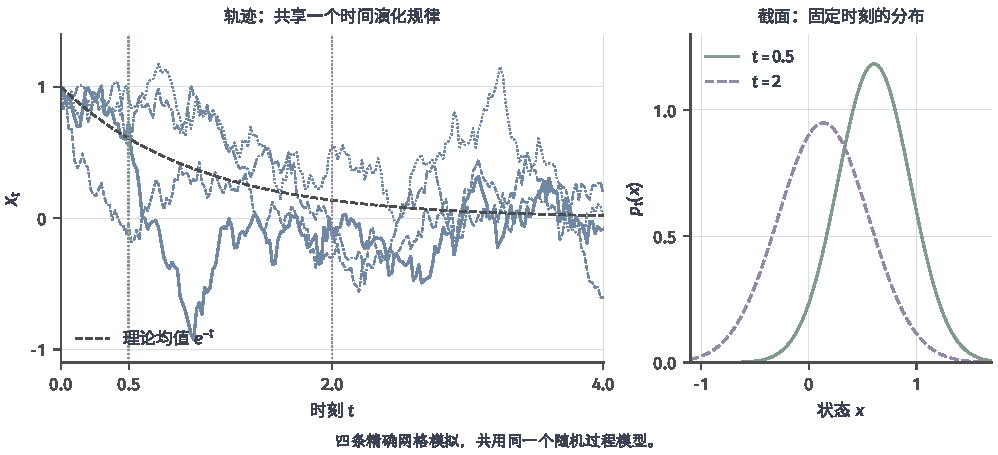
\includegraphics[width=\linewidth]{figures/00-shared/mathematical-preliminaries-lower/02-dynamical-systems-control-decision-and-games/matplotlib/action-state-ou-paths/figure.pdf}
  \caption{OU模型的路径与截面。取$\lambda=1,\sigma=0.6,X_0=1$，
 左侧为按精确高斯转移生成的四条网格轨迹与理论均值，右侧为$t=0.5,2$
 的解析边缘密度。折线只连接模拟网格点，不是可微的连续样本路径。
 截面给出单时刻概率，时间间的相关性还由共同噪声与转移决定。}
 \label{fig:action-state-ou-paths}
\end{figure*}

\subsection{给定初始分布下的状态分布求解}
逐路径的积分式不一定最适合回答“某时刻落在何处”的概率问题。
线性模型可传播少量矩，一般模型则要传播分布对测试函数的作用。
两者都来自同一演化规律，但矩摘要只有在附加分布条件下才是完整描述。

\subsubsection{线性演化下的均值与协方差求解}
对式~\eqref{eq:action-state-linear-sde-solution}，记
$\bm m_t=\mathbb E\bm X_t,\bm P_t=\operatorname{Cov}(\bm X_t)$。
随机积分为零均值、与初值独立，故
\begin{align*}
 \bm m_t&=\bm\Phi(t,0)\bm m_0+\int_0^t\bm\Phi(t,s)\bm c_s\,\mathrm ds,\\
 \bm P_t&=\bm\Phi(t,0)\bm P_0\bm\Phi(t,0)^\top
       +\int_0^t\bm\Phi(t,s)\bm G_s\bm G_s^\top\bm\Phi(t,s)^\top\,\mathrm ds.
\end{align*}
这里积分中的$\bm G_s\bm G_s^\top$是确定性矩阵。若扩散系数也随机，
就不能直接沿用这组确定性协方差公式；即使均方可积，取期望时也须保留
扩散系数的随机性及其与状态的关系。
两式绝对连续，对几乎处处的$t$有
\begin{align}
 \dot{\bm m}_t&=\bm A_t\bm m_t+\bm c_t,
       \label{eq:dynamical-linear-sde-mean}\\
 \dot{\bm P}_t&=\bm A_t\bm P_t+\bm P_t\bm A_t^\top+\bm G_t\bm G_t^\top.
       \label{eq:dynamical-linear-sde-covariance}
\end{align}
也可令$\widetilde{\bm X}=\bm X-\bm m$，直接用乘积Itô公式得到
\[
 \begin{split}
 \mathrm d(\widetilde{\bm X}\widetilde{\bm X}^{\top})
  ={}&(\bm A\widetilde{\bm X}\widetilde{\bm X}^{\top}
      +\widetilde{\bm X}\widetilde{\bm X}^{\top}\bm A^\top
      +\bm G\bm G^\top)\,\mathrm dt\\
    &+\bm G\,\mathrm d\bm W\,\widetilde{\bm X}^\top
      +\widetilde{\bm X}\,\mathrm d\bm W^\top\bm G^\top .
 \end{split}
\]
二阶矩界使随机积分取期望后消失，得到相同结论。
漂移传播已有不确定性，$\bm G\bm G^\top$持续注入新的不确定性；
后面的离散预测也有同样两项。

OU过程的初值只需平方可积并独立于驱动，就有
\begin{align}
 \mathbb E X_t&=\mathrm e^{-\lambda t}\mathbb E X_0,
       \label{eq:dynamical-ou-mean}\\
 \operatorname{Var}(X_t)&=\mathrm e^{-2\lambda t}\operatorname{Var}(X_0)
       +\frac{\sigma^2}{2\lambda}(1-\mathrm e^{-2\lambda t}).
       \label{eq:dynamical-ou-variance}
\end{align}
均值衰减；当$\sigma\neq0$时，方差趋于严格正值。对$f(x)=x^2$换元可再次核对：
$\mathrm d(X_t^2)=(-2\lambda X_t^2+\sigma^2)\,\mathrm dt
                 +2\sigma X_t\,\mathrm dW_t$。
若漏掉$\sigma^2\,\mathrm dt$，便会错误地认为持续噪声不留下方差。
当初始分布取$\mathcal N(0,\sigma^2/(2\lambda))$时，OU过程平稳；
一般初态只是在长期趋于该分布，而非每条路径趋于零。
$\sigma=0$时稳态退化为$\delta_0$。非高斯初值的有限时刻分布通常仍非高斯，
上面两个矩不能单独确定它。

\subsubsection{一般演化下的分布与密度求解}
设确定性系数与适当的解唯一性使$\bm X$成为Markov过程。
要知道分布怎样变化，可先观察任意光滑“读数”$\varphi(\bm X_t)$的短时期望。
\begin{definition}[Itô扩散的生成元]
 \label{def:dynamical-diffusion-generator}
 记$\mathbb E_{t,\bm x}$为从时刻$t$的状态$\bm x$出发的期望。
 对属于算子定义域的测试函数，生成元定义为
 \[
  (\mathcal L_t\varphi)(\bm x)
    =\lim_{h\downarrow0}
       \frac{\mathbb E_{t,\bm x}\varphi(\bm X_{t+h})-\varphi(\bm x)}h.
 \]
 对连续系数的扩散，令$\bm a=\bm\sigma\bm\sigma^\top$；
 在极限与期望可交换时，Itô公式给出
 \[
  \mathcal L_t\varphi=\bm b^\top\nabla\varphi+
                      \tfrac12\operatorname{tr}(\bm a\nabla^2\varphi).
 \]
\end{definition}
从积分Itô公式取条件期望，除以$h$再令$h\downarrow0$，即得最后一式。
例如取光滑紧支撑$\varphi$，并使系数在相关区域有界，可以先局部化来核对该极限。
若时间系数仅可测，则优先使用下面的积分弱式，不强求每个时刻的点态极限。

写$\mu_t$为状态分布。在鞅项可积且均值为零时，
\[
 \int\varphi\,\mathrm d\mu_t-\int\varphi\,\mathrm d\mu_0
     =\int_0^t\int\mathcal L_s\varphi\,\mathrm d\mu_s\,\mathrm ds.
\]
这是不要求密度存在的弱演化式。对有限活动的原计数驱动，还须加上
$\lambda[\varphi(\bm x+\bm\gamma(t,\bm x))-\varphi(\bm x)]$；
若方程用补偿驱动，则漂移算子相应增加
$\lambda[\varphi(\bm x+\bm\gamma)-\varphi(\bm x)
                          -\nabla\varphi^\top\bm\gamma]$。
离散跳跃由有限差算子表达，不是无条件多加一个扩散Hessian项。

若$\mu_t$有密度$p(t,\bm x)$，代入扩散弱式，漂移项分部积分一次，
扩散项分部积分两次，得到
\begin{align*}
 \int\varphi\,\partial_t p\,\mathrm d\bm x
  &=\int\left[\sum_i b_i\partial_i\varphi
            +\tfrac12\sum_{i,j}a_{i,j}\partial_{i,j}\varphi\right]p\,\mathrm d\bm x\\
  &=\int\varphi\left[-\sum_i\partial_i(b_ip)
           +\tfrac12\sum_{i,j}\partial_i\partial_j(a_{i,j}p)\right]\,\mathrm d\bm x .
\end{align*}
测试函数紧支撑时，无穷远处没有边界项；有界区域还需与模型匹配的边界条件。
因此得到\term{Fokker--Planck方程}
\begin{equation}
 \partial_t p=-\sum_i\partial_i(b_ip)
                  +\tfrac12\sum_{i,j}\partial_i\partial_j(a_{i,j}p).
 \label{eq:dynamical-fokker-planck}
\end{equation}
弱等式先成立；经典逐点形式另需$p$和系数的时间、空间正则性。
例如全空间光滑有界系数与一致椭圆扩散是获得正时间光滑密度的一组常用充分条件。
这里一致椭圆（uniformly elliptic）指存在固定$c>0$，使所讨论的时间与状态范围内，
\[
 \bm v^\top\bm a(t,\bm x)\bm v\geq c\|\bm v\|_2^2
 \quad\text{对所有 }\bm v\in\mathbb R^d\text{成立}.
\]
也就是每个方向的噪声强度都有同一个正下界。这比每个$(t,\bm x)$处分别正定更强：后者仍允许最小特征值随状态或时间趋于零。
退化扩散可能把概率留在低维集合，不能预先假定全维光滑密度。

把密度方程写成$\partial_t p=-\nabla\cdot\bm J$，其中
$J_i=b_ip-\frac12\sum_j\partial_j(a_{i,j}p)$。
在$p>0$处，令$\bm v=\bm J/p$，便得到概率流速度
\begin{equation}
 \bm v(t,\bm x)=\bm b(t,\bm x)
   -\tfrac12[\operatorname{div}\bm a(t,\bm x)
                         +\bm a(t,\bm x)\nabla_{\bm x}\log p(t,\bm x)],
 \quad
 (\operatorname{div}\bm a)_i=\sum_j\partial_j a_{i,j}.
 \label{eq:action-state-probability-flow}
\end{equation}
式中的$\bm s_t(\bm x)=\nabla_{\bm x}\log p(t,\bm x)$称为状态密度分数
（state score），表示在状态空间中对数密度上升最快的局部方向。
它对状态$\bm x$求导；前面统计几何中的参数得分对模型参数求导，两者的自变量及向量维数通常不同。
例如OU过程某个时刻的边缘为$\mathcal N(m_t,v_t)$且$v_t>0$时，
$s_t(x)=-(x-m_t)/v_t$，直接指向密度中心，距中心越远时幅度越大。
若此速度的ODE流存在、连续性方程适定，并具有同样初始密度及边界通量，
它便传播同样的边缘密度。若$\bm a$不依赖状态，散度项为零；
状态依赖时应按定义计算该项，不能直接省略。
上述匹配涉及各时刻的边缘分布：ODE在给定初态后无新的噪声，而扩散不断注入随机增量。

图~\ref{fig:reader-probability-flow-joint-law}给出一个可以直接计算的例子。
取$X_0\sim\mathcal N(0,1)$且与驱动Brownian运动$W$独立，并考虑
$\mathrm dX_t=-X_t\,\mathrm dt+\sqrt2\,\mathrm dW_t$。
这一OU扩散在每个时刻都保持$\mathcal N(0,1)$边缘，因而$a=2$、$s_t(x)=-x$；
代入式~\eqref{eq:action-state-probability-flow}得到$v=-x-(2/2)(-x)=0$。
对应ODE让每条轨迹停在各自初值上，也保持同一边缘分布。
左图中的密度因此重合，右图中的跨时协方差却不同：扩散逐渐失去对初态的相关性，
ODE则始终保留同一个初态。这说明所有单时刻边缘相同，仍不足以确定跨时联合规律。

\begin{figure}[htbp]
  \centering
  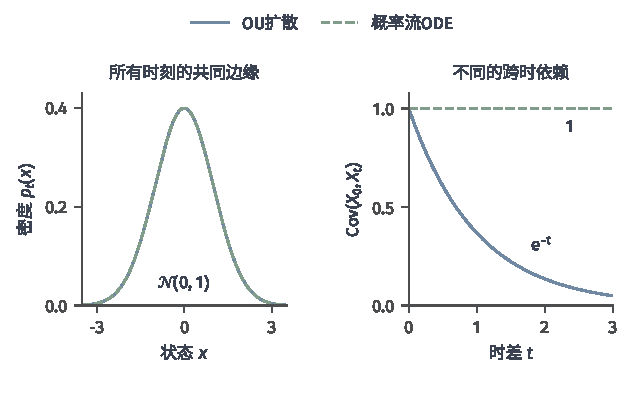
\includegraphics[width=107mm]{figures/00-shared/mathematical-preliminaries-lower/02-dynamical-systems-control-decision-and-games/matplotlib/reader-probability-flow-joint-law/figure.pdf}
  \caption{相同边缘密度与不同跨时依赖。教学模型的初态为$X_0\sim\mathcal N(0,1)$且与$W$独立，
  实线表示$\mathrm dX_t=-X_t\,\mathrm dt+\sqrt2\,\mathrm dW_t$，虚线表示对应的概率流ODE。
  左图两条解析密度在所有时刻都重合；右图中，OU扩散的
  $\operatorname{Cov}(X_0,X_t)=\mathrm e^{-t}$，而ODE因$X_t=X_0$使协方差恒为$1$。
  横轴和状态均采用无量纲单位；图中没有用有限样本拟合密度或协方差。}
  \label{fig:reader-probability-flow-joint-law}
\end{figure}

若终点分布已知或便于采样，可以从终点出发沿反方向生成路径。
概率流ODE只匹配每个时刻的边缘密度；要恢复相邻时刻的随机反向条件规律，
则需要时间反演的SDE。反向转移还取决于状态在原边缘中出现的概率，
因此不能只把漂移$b$取负。固定终点$T$，用正向反演时钟$s$定义
$\widehat{\bm X}_s=\bm X_{T-s}$。在正密度、系数和密度足够光滑、
扩散非退化及相应可积条件下，其反演滤过中的扩散矩阵为$\bm a(T-s,\bm x)$，
漂移为
\[
 \widehat{\bm b}(s,\bm x)
    =-\bm b(T-s,\bm x)+\operatorname{div}\bm a(T-s,\bm x)
                  +\bm a(T-s,\bm x)\nabla_{\bm x}\log p(T-s,\bm x).
\]
例如可先在远离奇异端点的紧时间区间上取光滑有界系数、一致椭圆矩阵、
正的光滑密度及局部可积的分数，并另保证反演方程无爆炸。
反演Brownian运动相对于反演历史定义，不能当作原Brownian路径简单反号。
这一结果还用到正反向转移的Bayes关系；前向密度方程本身不确定时间间联合规律。
上述反演形式及其生成建模用途见Song等的推导\scite{pgm-generative-song2021}
在生成模型中用估计分数替换真实分数，会再引入模型误差。

\paragraph{由条件路径构造边缘速度}
\label{sec:dynamical-conditional-path-velocity}
除了从给定SDE推出密度演化，还可以先构造一族容易采样的随机路径，
再问哪个只依赖当前状态的速度场能够传播相同的边缘分布。
用$s\in[0,1]$表示插值进度，设$\bm X_s$的样本路径几乎处处绝对连续，
路径速度$\bm U_s=\mathrm d\bm X_s/\mathrm ds$取联合可测版本，并满足
$\mathbb E\int_0^1\|\bm U_s\|_2\,\mathrm ds<\infty$。
记$\mu_s$为$\bm X_s$的分布，对几乎所有$s$取条件均值的可测版本
\begin{equation}
 \bm v_s(\bm x)=\mathbb E[\bm U_s\mid\bm X_s=\bm x].
 \label{eq:dynamical-conditional-path-velocity}
\end{equation}
它按当前状态汇总穿过该处的路径速度；不同路径可以带来不同速度，
条件均值只要求在$\mu_s$几乎处处有定义。

为何这样平均能够传播边缘分布，可以直接检查测试函数。
对$\varphi\in C_c^1(\mathbb R^d)$及$0\leq r\leq t\leq1$，
路径链式法则、Fubini定理及条件期望依次给出
\begin{equation}
 \begin{aligned}
 &\int\varphi\,\mathrm d\mu_t-\int\varphi\,\mathrm d\mu_r\\
 &\quad=\int_r^t\mathbb E[\nabla\varphi(\bm X_s)^\top\bm U_s]\,\mathrm ds\\
 &\quad=\int_r^t\int\nabla\varphi(\bm x)^\top\bm v_s(\bm x)
                                      \,\mathrm d\mu_s(\bm x)\,\mathrm ds.
 \end{aligned}
 \label{eq:dynamical-conditional-path-continuity}
\end{equation}
这是连续性方程的弱式，不要求$\mu_s$存在密度。

有密度$p_s$时，它写成$\partial_s p_s=-\nabla\cdot(p_s\bm v_s)$的分布意义等式；
逐点形式另需正则性。若速度场还满足使ODE流及连续性方程唯一的条件，
例如空间全局Lipschitz且线性增长、相关界在时间上可积，
从$\mu_0$出发求解$\mathrm d\bm Z_s/\mathrm ds=\bm v_s(\bm Z_s)$，
才可据此断言$\bm Z_s$具有$\mu_s$边缘。

例如从某个固定联合分布抽取端点$(\bm X_0,\bm X_1)$，并令
$\bm X_s=(1-s)\bm X_0+s\bm X_1$，则$\bm U_s=\bm X_1-\bm X_0$可逐样本计算。
若端点有有限二阶矩，对任意平方可积的候选速度$\bm w_s(\bm X_s)$，
条件均值的正交分解给出
\begin{equation}
 \begin{aligned}
 &\mathbb E\|\bm w_s(\bm X_s)-\bm U_s\|_2^2\\
 &\quad=\mathbb E\|\bm w_s(\bm X_s)-\bm v_s(\bm X_s)\|_2^2\\
 &\qquad+\mathbb E\|\bm U_s-\bm v_s(\bm X_s)\|_2^2.
 \end{aligned}
 \label{eq:dynamical-conditional-velocity-regression}
\end{equation}
第二项与候选速度无关，所以对易采样的路径速度做平方误差回归，
在总体上以该条件均值为最优预测；这正是条件流匹配使用的关系\scite{lipman2023flowmatching}。
单条插值路径是直线，并不要求边缘速度场的ODE轨迹也是直线，
也没有保证端点联合分布给出了最优传输。
若端点处的分布或速度出现奇异性，弱演化式仍须与ODE适定条件分开检查；
有限样本、受限函数族与数值积分的误差也不由上述恒等式消除。

\subsection{离散化条件下的轨迹求解}
\label{sec:dynamical-discretization-scan}

已知轨迹存在唯一，不代表能写出解析式——非线性方程往往求不出闭式解，只能在计算机上用离散的小步迭代去逼近它。这里要分清两种误差：从精确状态出发走一步，数值映射与真实流动的偏差叫一步局部误差；但数值方法每一步都从自己上一步算出的（已经带偏的）状态出发，误差会被动力学不断放大和累积，最终在终端形成全局误差。记从$t_n$到$t_{n+1}=t_n+h$的精确
流为$\varphi_{t_{n+1},t_n}$，数值方法以可计算的一步映射$\Psi_{h,t_n}$近似它。

\subsubsection{基于一般数值离散的轨迹求解}
显式Euler法在一步内使用当前斜率：
\begin{equation}
  \widehat{\bm x}_{n+1}
  =\widehat{\bm x}_n+h\bm f(t_n,\widehat{\bm x}_n).
  \label{eq:dynamical-forward-euler}
\end{equation}
这里已把给定输入吸收进$\bm f$。经典四阶Runge--Kutta法在同一步内评估四次：
\begin{align*}
  \bm k_1&=\bm f(t_n,\widehat{\bm x}_n),\\
  \bm k_2&=\bm f(t_n+h/2,\widehat{\bm x}_n+h\bm k_1/2),\\
  \bm k_3&=\bm f(t_n+h/2,\widehat{\bm x}_n+h\bm k_2/2),\\
  \bm k_4&=\bm f(t_n+h,\widehat{\bm x}_n+h\bm k_3),\\
  \widehat{\bm x}_{n+1}
    &=\widehat{\bm x}_n+\frac h6(\bm k_1+2\bm k_2+2\bm k_3+\bm k_4).
\end{align*}
固定有限时域，从精确初值出发，并假设精确轨迹、数值轨迹及各中间评估点都留在同一适用区域。
若该区域上的$\bm f$关于状态一致Lipschitz，精确解的二阶导数有界，
Euler法的全局误差为$O(h)$。对于上述四阶Runge--Kutta法，一组充分条件是
$\bm f$在该区域关于时间和状态具有至四阶连续有界偏导；
这保证一步误差为$O(h^5)$，有限时域累计后全局误差为$O(h^4)$。
较高阶意味着局部近似利用更多信息，也意味着每步更多函数评估；
不能只按步数比较成本\scite{math-hairer1993ode}

\begin{example}[连续稳定与数值稳定不是一回事]
  \label{ex:dynamical-scalar-discretization}
  对$\dot x=-\lambda x+u$，其中$\lambda>0$且$u$恒定，精确一步为
  \[
    x(t+h)=\mathrm e^{-\lambda h}x(t)
      +\frac{1-\mathrm e^{-\lambda h}}{\lambda}u.
  \]
  Euler一步为$\widehat x_{n+1}=(1-\lambda h)\widehat x_n+hu$。
  连续齐次系统始终指数衰减，Euler齐次递推却只有
  $|1-\lambda h|<1$，即$0<h<2/\lambda$时才衰减。
\end{example}
对这里的齐次泄漏递推，当$1<h\lambda<2$时，数值状态交替变号但幅值缩小；
当$h\lambda>2$时，它交替增长。若有恒定输入，同一判断作用于相对平衡点的偏差，
原状态本身不必在零的两侧交替。
若同一系统包含衰减很快与变化很慢的方向，显式方法可能为压住快方向而被迫采用
远小于慢变化尺度的步长，这就是刚性带来的主要计算困难。提高阶数不自动解除
稳定域限制；此处稳定域指使齐次数值解衰减的参数范围。
隐式方法改用包含下一状态的信息。例如隐式Euler（implicit Euler）满足
\[
 \widehat{\bm x}_{n+1}
 =\widehat{\bm x}_n+h f(t_{n+1},\widehat{\bm x}_{n+1}).
\]
未知的下一状态同时出现在等号两侧，因而每步都需解方程。
对相同的齐次泄漏模型，它给出
$\widehat x_{n+1}=\widehat x_n/(1+h\lambda)$，
当$h\lambda>0$时放大因子的模始终小于$1$。
这说明改变更新规则可以扩大该例的稳定域，代价是每步求解；
衰减得到保证也不等于任意大步长都能准确刻画轨迹。

\begin{figure*}[htbp]
  \centering
  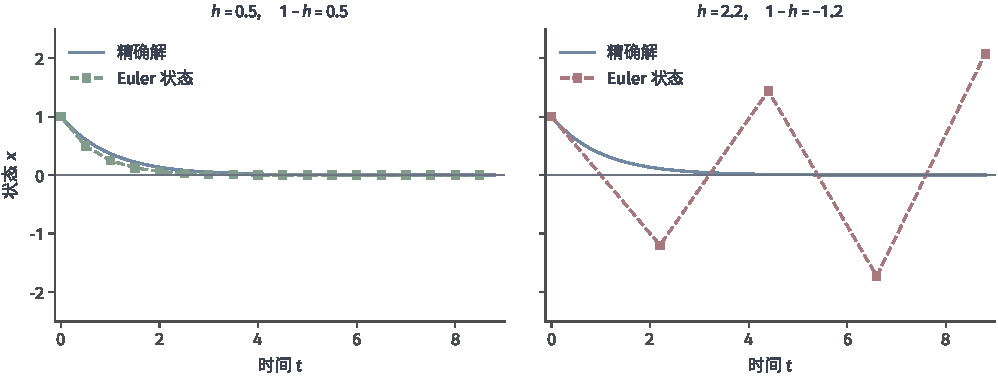
\includegraphics[width=\linewidth]{figures/00-shared/mathematical-preliminaries-lower/02-dynamical-systems-control-decision-and-games/matplotlib/dynamical-euler-stability/figure.pdf}
  \caption{教学方程$\dot x=-x$、$x(0)=1$的精确解与Euler近似。蓝色实线为精确解，
  方点为数值状态；左图绿色方点使用$h=0.5$并衰减，右图红色方点使用$h=2.2$并交替增长。两图采用相同坐标
  范围，连线只连接相邻数值状态。右图的发散来自步长，并非原连续系统不稳定。}
  \label{fig:dynamical-euler-stability}
\end{figure*}

\subsubsection{基于精确线性离散的轨迹求解}
前面的数值规则近似瞬时变化率，线性方程却允许在整段区间上求出精确转移。为使输入积分可算，假设
$[t_n,t_n+h)$内$\bm u(t)=\bm u_n$。将
式~\eqref{eq:dynamical-lti-variation-constants}限制到这一段，得到
\begin{align}
  \bm x_{n+1}&=\bm A_h\bm x_n+\bm B_h\bm u_n,
    \label{eq:dynamical-zoh-discrete}\\
  \bm A_h&=\mathrm e^{h\bm A},\qquad
  \bm B_h=\int_0^h\mathrm e^{(h-s)\bm A}\bm B\,\mathrm ds.
    \label{eq:dynamical-zoh-matrices}
\end{align}
这称为\term{零阶保持}离散化。精确性针对区间内保持不变的输入，不表示真实输入
在区间内任意变化时也精确。若$\bm A$可逆，
$\bm B_h=\bm A^{-1}(\mathrm e^{h\bm A}-\bm I)\bm B$；$\bm A$奇异时继续使用积分
形式，不人为引入不存在的逆。输入保持误差与计算矩阵指数的数值误差仍可能存在，
只是没有Euler式的时间截断误差。

\paragraph{连续随机模型的精确离散}
\label{sec:dynamical-exact-stochastic-discretization}
状态含有过程噪声时，还须把整段区间内积累的随机作用一起离散。
考虑常系数线性模型
\[
 \mathrm d\bm X_t=(\bm A\bm X_t+\bm B\bm u_n)\,\mathrm dt
                                  +\bm G\,\mathrm d\bm W_t,
 \qquad t\in[t_n,t_n+h),
\]
其中输入$\bm u_n$事先给定，$\bm W$为标准Brownian运动，初值与驱动独立。
由式~\eqref{eq:action-state-linear-sde-solution}，采样状态
$\bm X_n=\bm X_{t_n}$满足
\begin{equation}
 \begin{aligned}
 \bm X_{n+1}&=\bm A_h\bm X_n+\bm B_h\bm u_n+\bm\xi_n,\\
 \bm\xi_n&=\int_{t_n}^{t_n+h}
       \mathrm e^{(t_n+h-s)\bm A}\bm G\,\mathrm d\bm W_s
       \sim\mathcal N(\bm0,\bm Q_h),\\
 \bm Q_h&=\int_0^h\mathrm e^{r\bm A}\bm G\bm G^\top
                              \mathrm e^{r\bm A^\top}\,\mathrm dr.
 \end{aligned}
 \label{eq:dynamical-exact-stochastic-discretization}
\end{equation}

$\bm A_h,\bm B_h$仍由式~\eqref{eq:dynamical-zoh-matrices}给出。
确定性被积函数与Brownian独立增量使$\bm\xi_n$为高斯、独立于$t_n$以前的历史，
不相交区间的$\bm\xi_n$也相互独立；协方差积分来自Itô等距。
记$\bm P_n=\operatorname{Cov}(\bm X_n)$，平方可积初值下有
$\bm P_{n+1}=\bm A_h\bm P_n\bm A_h^\top+\bm Q_h$。
这给出网格上的精确高斯转移，但初始分布非高斯时，不能把全部状态边缘也称为高斯。
它为后面的离散滤波模型确定了过程噪声协方差$\bm Q_h$\scite{pgm-dynamic-sarkka2023}。

以一维位置$R_t$与速度$V_t$为例，连续白加速度模型写成
\[
 \mathrm dR_t=V_t\,\mathrm dt,\qquad
 \mathrm dV_t=\sqrt q\,\mathrm dW_t,\qquad q>0.
\]
这里“白加速度”通过速度的Brownian增量定义，不把Brownian路径当作普通可微函数。
取$\bm X_t=(R_t,V_t)^\top$，则
$\bm A=\bigl(\begin{smallmatrix}0&1\\0&0\end{smallmatrix}\bigr)$、
$\bm G=(0,\sqrt q)^\top$，且
$\mathrm e^{r\bm A}\bm G=\sqrt q(r,1)^\top$，于是
\begin{equation}
 \bm A_h=\begin{pmatrix}1&h\\0&1\end{pmatrix},\qquad
 \bm Q_h=q\begin{pmatrix}h^3/3&h^2/2\\h^2/2&h\end{pmatrix}.
 \label{eq:dynamical-white-acceleration-discretization}
\end{equation}
转移均值按匀速前进，随机作用同时产生位置方差、速度方差及两者的协方差。
例如位置方差由$\int_0^h qr^2\,\mathrm dr=qh^3/3$给出，
因此改变采样间隔时，不能只给一个固定噪声方差而保持其他项不变。

另一种模型在每个采样区间内保持同一个随机加速度$A_n$，
各$A_n$相互独立且独立于初态，均值为零、方差为$\sigma_a^2>0$。
普通积分给出该段的随机位移与速度增量
$\bm\xi_n=(h^2/2,h)^\top A_n$，故
\begin{equation}
 \bm Q_h^{\mathrm{hold}}
   =\sigma_a^2\begin{pmatrix}h^4/4&h^3/2\\h^3/2&h^2\end{pmatrix}.
 \label{eq:dynamical-held-acceleration-covariance}
\end{equation}
它只由一个随机幅度推动，协方差秩为$1$；式~\eqref{eq:dynamical-white-acceleration-discretization}
在$h>0$时则为满秩。$q$是单位时间的速度增量方差，
$\sigma_a^2$是每段加速度幅度的方差，两者量纲与区间内的随机假设都不同，
不能因都称为“匀速加噪声”就互换这两组协方差。

\subsubsection{基于几何离散的保守轨迹求解}
\label{sec:dynamical-hamiltonian-geometric-integration}
保守方程（如无摩擦的天体运动）的数值计算有一个特殊要求：除了把每条轨迹算得尽量准，还希望离散格式不破坏原系统的几何性质——能量不无故增减、相空间体积不膨胀收缩、时间反演后能原路返回。普通的 Euler 格式哪怕每步误差很小，长期模拟也可能让能量系统性漂移，从而得到完全错误的定性行为。先沿Hamilton方程求出能量和体积的变化，再据此构造离散映射；保持某种结构不等于每一步都精确，也不自动保证任意步长稳定。

\paragraph{精确演化的能量保持}
\begin{theorem}[Hamilton能量守恒]
  \label{thm:dynamical-hamiltonian-energy-conservation}
  若$H$连续可微、不显含时间，且Hamilton方程的解在所考察区间存在，则
  \[
    H(\bm q(t),\bm p(t))=H(\bm q(0),\bm p(0)).
  \]
\end{theorem}
\begin{proof}
  沿解使用链式法则和式~\eqref{eq:dynamical-hamilton-equations}，
  \[
    \frac{\mathrm dH}{\mathrm dt}
    =\nabla_{\bm q}H^\top\dot{\bm q}
      +\nabla_{\bm p}H^\top\dot{\bm p}
    =\nabla_{\bm q}H^\top\nabla_{\bm p}H
      -\nabla_{\bm p}H^\top\nabla_{\bm q}H=0.
  \]
  积分即得结论。
\end{proof}
因此轨迹被限制在初始能量面上，而不是向能量极小值下降。若$H$显含时间，
同一计算只给出$\mathrm dH/\mathrm dt=\partial_tH$。
守恒本身也不保证全局存在或位置有界：自由粒子$H=p^2/2$保持动量与能量，
但$p\neq0$时$q(t)=q(0)+pt$没有界。只有能量子水平集紧、向量场局部存在条件
持续有效等附加条件，才可利用守恒排除有限时间逃逸。

\paragraph{精确演化的辛结构与体积保持}
能量只给轨迹上的标量限制，仍未说明一小团相邻初态怎样变形。为比较方向之间的
关系，取相空间坐标$\bm z=(\bm q^\top,\bm p^\top)^\top$及前述矩阵$\bm J$。
只有一对位置、动量时，两条小扰动\((u_q,u_p)\)、\((v_q,v_p)\)张成的有向面积为\(u_qv_p-u_pv_q\)。保持它，要求变换同时尊重位置与动量的配对；多对坐标时，把各对的这一面积相加，就得到下面由\(\bm J\)表示的双线性形式。于是要检查的不只是能量数值，还包括相邻方向之间的这种配对是否保持。
\begin{definition}[标准辛形式与辛映射]
  \label{def:dynamical-symplectic-form-map}
  对$\bm u,\bm v\in\mathbb R^{2d}$，标准\term{辛形式}为
  $\omega(\bm u,\bm v)=\bm u^\top\bm J\bm v$。
  若$C^1$映射$\psi$在定义域每一点的Jacobian矩阵$\bm G=\nabla\psi$满足
  \begin{equation}
    \bm G^\top\bm J\bm G=\bm J,
    \label{eq:dynamical-symplectic-map}
  \end{equation}
  则称其为辛映射。
\end{definition}
该等式表示任意两方向经映射后具有相同的辛形式值。一个位置和一个动量时，
它就是有向面积；多对坐标时，它还约束共轭方向之间的配对，强于只记录总体积。

设$H\in C^2$、$\bm F=\bm J\nabla H$。把初态$\bm z_0$映到时刻$t$状态的映射
记为$\varphi_t(\bm z_0)=\bm z(t;\bm z_0)$，称为精确流（exact flow）。
以下限制在所考察初态邻域内的解共同存在的局部时间区间。
固定$t$时，这个映射的自变量是初态；$C^1$向量场使它对初态可微。
记$\bm G_t=\nabla\varphi_t(\bm z_0)$，它把初态的小扰动转成当前状态的一阶扰动。
对积分方程关于初值求导得到变分方程
\[
  \dot{\bm G}_t=\nabla\bm F(\bm z(t))\bm G_t,\qquad \bm G_0=\bm I.
\]
初始映射$\varphi_0$是恒等映射，所以$\bm G_0=\bm I$。
反向时间的唯一解给出流的局部逆，所以$\bm G_t$可逆。由Jacobi行列式公式，
\[
  \frac{\mathrm d}{\mathrm dt}\log|\det\bm G_t|
  =\operatorname{tr}(\nabla\bm F)
  =\operatorname{tr}(\bm J\nabla^2H)=0.
\]
最后一个等号来自反对称矩阵与对称矩阵的乘积迹为零。初始行列式为$1$，
故$\det\bm G_t=1$，精确流保持相空间体积及其定向。

还可直接验证更强的辛性。写$\bm S=\nabla^2H=\bm S^\top$，则
\[
  \begin{aligned}
    \frac{\mathrm d}{\mathrm dt}(\bm G_t^\top\bm J\bm G_t)
    &=\bm G_t^\top[(\bm J\bm S)^\top\bm J
                         +\bm J(\bm J\bm S)]\bm G_t\\
    &=\bm G_t^\top(\bm S-\bm S)\bm G_t=\bm0.
  \end{aligned}
\]
初值为$\bm J$，所以精确流满足式~\eqref{eq:dynamical-symplectic-map}。
对该式取行列式也给出$(\det\bm G_t)^2=1$，结合从恒等映射连续出发，
再次得到$\det\bm G_t=1$。

反向推断却不成立。在$(q_1,q_2,p_1,p_2)$坐标下，
$\operatorname{diag}(2,1,1,1/2)$的行列式为$1$，但它把第一对位置动量的面积
乘以$2$，第二对乘以$1/2$，不保持标准辛形式。总体积不变允许不同配对之间
互相抵消；辛性不允许这种抵消代替各方向对的结构。

\paragraph{离散演化的结构保持}
对于可分Hamilton量，势能子系统保持位置、只改变动量；动能子系统保持动量、
只改变位置。两者各自可精确求解，因而可用对称分裂组成一步蛙跳：
\begin{align}
  \bm p_{n+1/2}&=\bm p_n-\frac h2\nabla U(\bm q_n),
    \label{eq:dynamical-leapfrog-half-momentum}\\
  \bm q_{n+1}&=\bm q_n+h\bm M^{-1}\bm p_{n+1/2},
    \label{eq:dynamical-leapfrog-position}\\
  \bm p_{n+1}&=\bm p_{n+1/2}-\frac h2\nabla U(\bm q_{n+1}).
    \label{eq:dynamical-leapfrog-final-momentum}
\end{align}
它是“动量半步、位置整步、动量半步”，不是把两条方程各做一次独立Euler更新。
令
$S_U^c(\bm q,\bm p)=(\bm q,\bm p-c\nabla U(\bm q))$、
$S_K^h(\bm q,\bm p)=(\bm q+h\bm M^{-1}\bm p,\bm p)$。
若$U\in C^2$，相应Jacobian为
\[
  \bm G_U=\begin{bmatrix}\bm I&\bm0\\-c\nabla^2U&\bm I\end{bmatrix},
  \qquad
  \bm G_K=\begin{bmatrix}\bm I&h\bm M^{-1}\\\bm0&\bm I\end{bmatrix}.
\]
三角结构使二者行列式均为$1$；$\nabla^2U$和$\bm M^{-1}$的对称性又给出
$\bm G_U^\top\bm J\bm G_U=\bm J$及
$\bm G_K^\top\bm J\bm G_K=\bm J$。故复合
$\Psi_h=S_U^{h/2}\circ S_K^h\circ S_U^{h/2}$保持体积且为辛映射。

每个子步换成负步长便是其逆，三步的对称排列使
$\Psi_h^{-1}=\Psi_{-h}$。若$R(\bm q,\bm p)=(\bm q,-\bm p)$是动量翻转，则还有
\[
  R\circ\Psi_h\circ R=\Psi_{-h}=\Psi_h^{-1}.
\]
因此这里的时间反演关系涉及动量翻转。把同一个映射连续应用两次便回到原态，
即$\Psi_h\circ\Psi_h=\operatorname{id}$，才称该映射为对合（involution）；
上面的逆映射关系不要求$\Psi_h$满足这个条件。
在足够光滑和固定有限时域下，蛙跳具有二阶全局精度。
下面的谐振子例将直接算出一个精确保持的修正二次型，说明该例的原能量为何有界而不必恒定。
这一具体结论依赖步长范围与线性结构；辛性本身不保证一般Hamilton量每步完全相同。

\begin{example}[谐振子的精确与数值轨道]
  \label{ex:dynamical-harmonic-oscillator}
  取$U(q)=q^2/2,M=1$，精确解沿$q^2+p^2$的等值圆运动。蛙跳一步为
  \[
    \begin{bmatrix}q_{n+1}\\p_{n+1}\end{bmatrix}
    =
    \begin{bmatrix}1-h^2/2&h\\-h+h^3/4&1-h^2/2\end{bmatrix}
    \begin{bmatrix}q_n\\p_n\end{bmatrix}.
  \]
  更新矩阵的行列式为$1$、迹为$2-h^2$。当$0<h<2$时，其特征值是不同的
  单位模共轭数，并精确保持
  $(1-h^2/4)q_n^2+p_n^2$；这是一族椭圆，不是原来的能量圆。
  例如从$(1,0)$出发取$h=1$，一步得到$(1/2,-3/4)$，
  原能量从$1/2$变成$13/32$，却仍保持上述修正二次型。
  $h>2$时出现模大于$1$的特征值，$h=2$时还有退化导致的增长方向。
\end{example}
所以可逆、辛、体积保持与数值稳定分别需要检查。将这类轨迹用于随机采样时，
能量误差还需接受校正，不能把几何积分器直接当作精确采样器。

\subsubsection{基于随机离散的有限时域轨迹模拟}
固定$T$，取$t_k=kh$、$n=T/h$为整数，初值
$\widehat{\bm X}_0=\bm X_0$。Euler--Maruyama方法冻结每段左端的系数：
\begin{equation}
 \widehat{\bm X}_{k+1}=\widehat{\bm X}_k+
    h\bm b(t_k,\widehat{\bm X}_k)
    +\bm\sigma(t_k,\widehat{\bm X}_k)\sqrt h\,\bm\varepsilon_k,
 \qquad \bm\varepsilon_k\overset{\mathrm{iid}}{\sim}\mathcal N(\bm0,\bm I_m).
 \label{eq:dynamical-euler-maruyama}
\end{equation}
新噪声与初值、先前噪声独立。扩散项乘$\sqrt h$，才能每单位时间累计有限方差；
随机逼近中的步长乘观测误差通常是$h\xi_k$，方差尺度为$h^2$，两者不是同一极限。

Poisson驱动须另生成$\Delta N_k\sim\operatorname{Pois}(\lambda h)$，
并按驱动假设与Brownian增量独立。网格法用
$\bm\gamma(t_k,\widehat{\bm X}_k)\Delta N_k$冻结该段跳幅；
补偿版本改用$\Delta N_k-\lambda h$。当一段内有多个事件且跳幅依赖状态时，
这种冻结不同于逐事件更新。
事件适配法则依次采样独立$\operatorname{Exp}(\lambda)$等待时间，
把跳时插入网格，在事件间模拟扩散、在事件处用跳前状态更新。
这里Brownian增量仍按各段实际长度采样，不能用高斯增量冒充跳跃计数。

\section{演化与计算序列的收敛}
\label{sec:action-state-convergence}
温度经过很久以后趋向什么，是演化时间增长的问题；固定一小时的轨迹能否被更细网格准确计算，是步长缩小的问题；噪声观测推动的求根算法是否找到根，则让算法迭代次数增长。这三种极限固定的对象不同。长期采样还要分别比较逐时刻的分布与一条路径的时间平均。

\subsection{长时间演化下的状态极限}
为什么要关心平衡点附近的稳定性？因为真实系统几乎不可能从精确的理想状态出发：初始测量总有误差，运行中也会受到意外扰动。如果相邻初值产生的轨迹很快分道扬镳，那么对初值的一点无知就会让长期预测完全失效；反之若偏差始终很小甚至逐渐消失，用近似初值做预测才有意义。
设某状态开始时完全不动，仍要分别问：微小初值误差会不会放大、会不会最终消失、消失是否有统一指数速度。前两问已不同于只看一条轨迹是否趋向某点，第三问还增加了速度要求。下面先找出不动状态，再用对邻域内全部初值的条件区分这些性质。
\begin{definition}[平衡点与稳定性]
  \label{def:dynamical-equilibrium-stability}
  考虑局部Lipschitz自治方程$\dot{\bm x}=\bm f(\bm x)$。
  满足$\bm f(\bm x^\star)=\bm0$的状态称为平衡点。以下性质均要求所涉及初值的
  解对全部$t\geq0$存在。

  平衡点在Lyapunov意义下\term{稳定}，是指对每个$\varepsilon>0$，存在
  $\delta>0$，使$\|\bm x(0)-\bm x^\star\|<\delta$蕴含
  $\|\bm x(t)-\bm x^\star\|<\varepsilon$对全部$t\geq0$成立。
  它具有局部吸引性，是指存在$r>0$，使所有
  $\|\bm x(0)-\bm x^\star\|<r$的解都趋于$\bm x^\star$。
  同时稳定且有局部吸引性称为\term{渐近稳定}。
  若存在$r,C,\alpha>0$，对上述$r$邻域内全部初值和$t\geq0$都有
  \[
    \|\bm x(t)-\bm x^\star\|_2
    \leq C\mathrm e^{-\alpha t}\|\bm x(0)-\bm x^\star\|_2,
  \]
  则称为局部指数稳定。若同一估计对全部初值成立，则称为全局指数稳定。
\end{definition}
离散时间把$t\geq0$换成非负整数，平衡条件换成
$F(\bm x^\star)=\bm x^\star$，指数因子可写成$q^t$，其中$0<q<1$。
“最终接近”与“始终不远离”分别对应吸引与稳定；不能只展示一条收敛轨迹，
便省去邻域内全部初值的量词。指数条件还要求$C,\alpha$在整个邻域统一。

\begin{table*}[htbp]
  \centering
  \begin{tabularx}{\linewidth}{lXXX}
    \toprule
    方程与原点 & 小初值始终小 & 轨迹趋于原点 & 统一指数衰减\\
    \midrule
    $\dot x=0$ & 是，状态保持初值 & 否，非零初值不动 & 否\\
    $\dot x=-x^3$ & 是，$|x(t)|$不增 & 是，代数衰减 & 否\\
    $\dot x=-x$ & 是 & 是 & 是，$|x(t)|=\mathrm e^{-t}|x(0)|$\\
    \bottomrule
  \end{tabularx}
  \caption{零输入下原点的稳定性质。第二行的解为
  $x(t)=x(0)/\sqrt{1+2x(0)^2t}$，它回到原点但不具有统一指数速度。
  三种方程均有全局解，比较不涉及数值离散。}
  \label{tab:dynamical-stability-types}
\end{table*}

有些轨迹不趋于一点，而是长期绕着一个集合运动。对此需要集合版本的描述。
\begin{definition}[不变集合与轨迹极限集]
  \label{def:dynamical-invariant-limit-sets}
  设$\Phi_t$是局部Lipschitz自治方程的流，并要求所述集合上的解正向全局存在。
  若$\Phi_t(\Omega)\subseteq\Omega$对全部$t\geq0$成立，则$\Omega$为
  \term{正向不变集}。若$\Phi_t(M)=M$对全部$t\geq0$成立，则$M$为
  \term{不变集}；这还要求集合内每一点有任意长时间以前的集合内前像，等价于
  每点都位于始终留在集合内的完整轨迹上。
  对正向有界轨迹，定义其\term{$\omega$极限集}为
  \[
    \omega(\bm x_0)=
    \{\bm z:\text{存在 }t_j\to\infty\text{ 使 }\bm x(t_j)\to\bm z\}.
  \]
\end{definition}
正向不变集限制一批初值的全部未来，极限集则记录一条轨迹在越来越晚的时刻反复
靠近的状态。趋于集合指到该集合的距离趋零，不要求在集合内部停止运动。

为避免逐条求解轨迹，可以寻找一个非负标量\(V\)来度量偏离平衡点的程度。若它沿轨迹不增，轨迹就不能穿越更高的子水平集；要据此得到有界性，还需所用子水平集有界，并保证解可继续存在。非增本身不能推出状态最终到达\(V\)的最低点：例如旋转系统\(\dot x_1=-x_2,\dot x_2=x_1\)取\(V=(x_1^2+x_2^2)/2\)，则\(\dot V=-x_1x_2+x_2x_1=0\)，非零初值的轨迹却始终沿圆周运动。要证明趋向平衡，还须严格下降等条件，或按后面的LaSalle原理检查零导数集合内最大的完整不变集。以原点为平衡，
$V\in C^1(D)$若满足$V(\bm0)=0$且非零点上$V>0$，称为正定的Lyapunov候选。
“候选”只说明它有合适的空间形状，还没有证明沿轨迹的变化方向。
\begin{definition}[Lyapunov函数]
  \label{def:dynamical-lyapunov-function}
  对$\dot{\bm x}=\bm f(\bm x)$，若上述正定候选还满足
  $\dot V(\bm x):=\nabla V(\bm x)^\top\bm f(\bm x)\leq0$，
  则称其为该邻域内的\term{Lyapunov函数}；若非零点处严格小于零，
  则称为严格Lyapunov函数。
\end{definition}
它不必等于物理能量。离散方程相应检查
$V(F(\bm x))-V(\bm x)$。正定性使“小能量”确实限制所有状态方向，
非增性才保证轨迹不能穿越更高的能量边界。下面的线性与非线性判据共同使用这两项。

\subsubsection{平衡邻域内的状态极限}
对已经定义的平衡点，吸引性直接问邻域内的轨迹是否回到该点。温度模型的零输入偏差满足\(e_{t+1}=0.8e_t\)，因而\(e_t=0.8^t e_0\to0\)；连续模型\(\dot e=-\lambda e\)、\(\lambda>0\)则给出\(e(t)=e^{-(t-t_0)\lambda}e(t_0)\to0\)。这些显式公式同时控制整个邻域的初值，不能用一条轨迹的图形代替这样的量词。

一般非线性方程未必有解析式。若能找到正定函数，并证明它沿每条轨迹严格下降，就能在合适邻域内证明趋向平衡；其稳定性与吸引性论证在第~\ref{sec:action-state-nonlinear-stability}节一并给出。下降函数仅有非正导数时，还需检查轨迹是否能停留在较大的零导数集合中。

\subsubsection{不变区域内的极限集合}
机械能常只在某些方向上直接耗散，导致$\dot V=0$的集合远大于平衡点。
这时应问：轨迹能否一直留在这个集合中？LaSalle原理把这个问题转成极限集合判据。
\begin{theorem}[LaSalle不变性原理]
  \label{thm:dynamical-lasalle-invariance}
  设自治向量场$\bm f$局部Lipschitz，$\Omega$紧且正向不变，
  $V$在包含$\Omega$的开邻域上为$C^1$，并有$\dot V\leq0$。
  令$E=\{\bm x\in\Omega:\dot V(\bm x)=0\}$，$M$为$E$中最大不变集，
  则从$\Omega$出发的每条轨迹满足
  $\operatorname{dist}(\bm x(t),M)\to0$。
\end{theorem}
\begin{proof}
  紧性排除有限时间逃逸，也使$\omega(\bm x_0)$非空且紧。
  沿轨迹的$V$单调不增且有下界，故趋于$v_\infty$。
  对极限点$\bm z=\lim_j\bm x(t_j)$，连续性给出$V(\bm z)=v_\infty$。

  对固定$s\geq0$，在这段有限时间内对两条解的积分方程作差，再用引理~\ref{lem:action-state-gronwall}，得到流对初值的连续依赖。因此
  $\bm x(t_j+s)\to\Phi_s(\bm z)$，故
  $\Phi_s(\omega(\bm x_0))\subseteq\omega(\bm x_0)$。
  反过来，充分大的$j$有$t_j>s$。紧性允许从$\bm x(t_j-s)$取收敛子列，
  其极限$\bm w$属于$\omega(\bm x_0)$，且$\Phi_s(\bm w)=\bm z$。
  因此$\Phi_s(\omega(\bm x_0))=\omega(\bm x_0)$，这里得到的是完整不变性，
  而非仅正向不变性。

  $V$在极限集上恒为$v_\infty$，从其中任一点出发的轨迹仍在该集合，
  所以沿轨迹导数为零。于是$\omega(\bm x_0)$是$E$内的不变集，必包含于$M$。
  若到$M$的距离不趋零，就有$\varepsilon>0$及$t_j\to\infty$使距离至少为
  $\varepsilon$。紧性再给出收敛子列，其极限属于$\omega(\bm x_0)\subseteq M$，
  与此距离下界矛盾。
\end{proof}

\begin{example}[阻尼振子的零导数集合]
  \label{ex:dynamical-damped-oscillator-lasalle}
  对$\dot q=p,\dot p=-q-cp$，其中$c>0$，取$V=(q^2+p^2)/2$，则
  $\dot V=q p+p(-q-cp)=-cp^2\leq0$。
  零导数集合为$p=0$；但其上$q\neq0$的点满足$\dot p=-q\neq0$，
  马上离开该直线。因此零导数集合中最大不变集只有原点。
  每个能量子水平集均紧且正向不变，LaSalle原理遂给出所有轨迹趋于原点。
\end{example}

\begin{figure}[htbp]
  \centering
  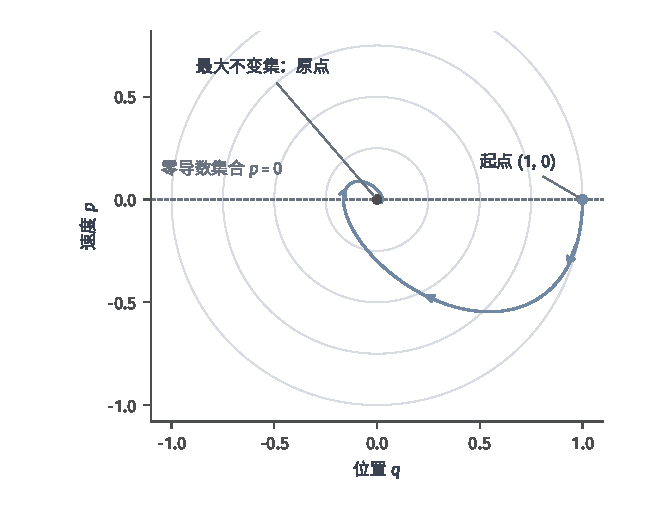
\includegraphics[width=\linewidth]{figures/00-shared/mathematical-preliminaries-lower/02-dynamical-systems-control-decision-and-games/matplotlib/reader-lasalle-zero-set/figure.pdf}
  \caption{阻尼振子$\dot q=p,\dot p=-q-p$从$(1,0)$出发的精确轨迹。
  蓝色轨迹覆盖$t=0$至$12$，箭头指示时间；灰色虚线为$\dot V=0$的直线$p=0$，
  浅灰圆为能量参考等值线。起点虽在零导数集合上，初始速度$(0,-1)$却将它带离
  该集合；能一直留在其中的完整轨迹只有原点。}
  \label{fig:reader-lasalle-zero-set}
\end{figure}
能量非增先限制活动区域，动力学再排除不能持续停留的零导数点。
把整个$E$直接称为“最终状态”，会丢掉LaSalle论证中最关键的一步。

\subsection{步长缩小下的轨迹逼近}
固定真实方程、初值和有限时域，改变数值网格的步长\(h\)。确定性计算比较网格状态与精确轨迹；随机计算可以使用同一噪声比较状态，也可以只比较测试函数的期望。前一种随机误差称强误差，后一种称弱误差，两者的尺度和条件不同。

\subsubsection{确定性演化下的离散误差}
\begin{theorem}[Euler法的有限时域全局误差]
  \label{thm:dynamical-euler-global-error}
  设$\bm f$在包含精确轨迹与Euler轨迹的区域内关于状态具有Lipschitz常数$L$，
  精确解二阶连续可微，且$\|\ddot{\bm x}(t)\|_2\leq M$。
  从精确初值出发，若$t_n=t_0+nh\leq t_0+T$，则$L>0$时
  \[
    \|\widehat{\bm x}_n-\bm x(t_n)\|_2
      \leq\frac{Mh}{2L}(\mathrm e^{LT}-1).
  \]
  $L=0$时相应上界为$MTh/2$。
\end{theorem}
\begin{proof}
  Taylor公式给出
  $\bm x(t_{n+1})=\bm x(t_n)+h\bm f(t_n,\bm x(t_n))+\bm\tau_n$，
  其中$\|\bm\tau_n\|_2\leq Mh^2/2$。记
  $\bm e_n=\widehat{\bm x}_n-\bm x(t_n)$，相减并用Lipschitz条件得
  \[
    \|\bm e_{n+1}\|_2\leq(1+Lh)\|\bm e_n\|_2+Mh^2/2.
  \]
  从$\bm e_0=\bm0$展开，
  $\|\bm e_n\|_2\leq(Mh^2/2)\sum_{j=0}^{n-1}(1+Lh)^j$。
  $L>0$时求几何和，并用$(1+Lh)^n\leq\mathrm e^{Lnh}\leq\mathrm e^{LT}$，
  即得所述界；$L=0$时直接使用$nh\leq T$。
\end{proof}
这也是离散Grönwall估计的一个具体推导。局部$O(h^2)$经约$T/h$步累计成为
全局$O(h)$，而动力学决定这些误差随后放大多少。更一般地，若数值映射的
Lipschitz常数不超过$L_h$、沿精确轨迹的局部误差不超过$\tau_h$，则
\[
  \|\bm e_{n+1}\|\leq L_h\|\bm e_n\|+\tau_h,\qquad
  \|\bm e_n\|\leq L_h^n\|\bm e_0\|+\tau_h\sum_{j=0}^{n-1}L_h^j.
\]
有限精度中的舍入误差也会通过同一传播机制进入后续状态。不断减小步长能减少
截断误差，却增加运算次数，未必无限改善最后精度。

\subsubsection{同一噪声下的随机轨迹误差}
同一次噪声实现会产生一条真轨迹和一条数值轨迹。要比较两条路径的状态误差，网格算法必须使用真轨迹的同一驱动，即令
$\sqrt h\,\bm\varepsilon_k=\bm W_{t_{k+1}}-\bm W_{t_k}$。
对自治系数，在全局Lipschitz、线性增长和$\bm X_0\in L^2$条件下，
固定有限时域有
\[
 \max_{0\leq k\leq n}
   \bigl(\mathbb E\|\bm X_{t_k}-\widehat{\bm X}_k\|^2\bigr)^{1/2}
     \leq C_T h^{1/2}.
\]
显式时间依赖时，一组充分条件是统一状态Lipschitz，并有
$\|\bm b(t,\bm x)-\bm b(s,\bm x)\|
 +\|\bm\sigma(t,\bm x)-\bm\sigma(s,\bm x)\|_{\mathrm F}
 \leq K(1+\|\bm x\|)|t-s|^{1/2}$。
常数依赖$T$和系数界，不是无限时域的统一保证。

估计机制与存在性证明相连。定义连续插值
\[
 \begin{split}
 \widehat{\bm X}_t={}&\bm X_0+
    \int_0^t\bm b(\eta(s),\widehat{\bm X}_{\eta(s)})\,\mathrm ds\\
 &+\int_0^t\bm\sigma(\eta(s),\widehat{\bm X}_{\eta(s)})\,\mathrm d\bm W_s,
 \end{split}
\]
其中$\eta(s)=t_{\lfloor s/h\rfloor}$，插值在网格上等于算法值。
增长界先给出统一二阶矩，并由等距得到
$\sup_{s\leq T}\mathbb E\|\widehat{\bm X}_s-\widehat{\bm X}_{\eta(s)}\|^2
\leq C_T h$。相减积分方程，用Lipschitz、最大不等式和时间正则性得
\[
 E(t):=\mathbb E\sup_{r\leq t}\|\bm X_r-\widehat{\bm X}_r\|^2
       \leq C_T\int_0^tE(s)\,\mathrm ds+C_T h.
\]
Grönwall给出$E(T)\leq C'_T h$，开方即得强半阶。
加性噪声等结构可能提高阶数，但不是一般乘性噪声的保证；
跳跃扩展还需另核对跳幅、驱动耦合与事件处理。

\subsubsection{测试函数下的随机模拟误差}
若只查询终点读数的平均，目标变成测试函数$\varphi$在真终点和数值终点下的期望差，不必把两条路径逐次配对。控制这一弱误差需要能对转移作用作展开。一组方便的自治充分条件是漂移、
扩散与测试函数$\varphi$具有至四阶连续有界导数，并满足增长和所需矩条件；
更保守地可取它们本身及至四阶导数均有界。此时
\[
  |\mathbb E\varphi(\bm X_T)-\mathbb E\varphi(\widehat{\bm X}_n)|
        \leq C_{\varphi,T}h.
\]
其机制是对剩余期望函数
$u(t,\bm x)=\mathbb E_{t,\bm x}\varphi(\bm X_T)$作局部展开。
在其相应导数有界的条件下，精确转移与一次Euler转移都给出
$u+h\mathcal L u+O(h^2)$。把每步的期望差望远镜相加，
$n=T/h$个局部$O(h^2)$误差累计为$O(h)$。
这里引用标准弱收敛结果，导数与矩条件用于保证展开余项统一可积；
不能仅凭二阶矩和状态Lipschitz就断言弱一阶\scite{math-kloeden1992numerical-sde}

弱阶较高不说明两条样本轨迹更接近。例如独立生成的两个同分布终点对所有可积
测试函数期望完全相同，彼此状态距离却不为零。有限时间弱误差还不能直接交换
$h\downarrow0$与$T\uparrow\infty$，长期步长偏差必须单独分析。

\subsection{随机近似下的迭代序列收敛}
\label{sec:stoch-approximation-markov-noise}

有些递推状态不是房间温度，而是希望逐步求出的参数。以最简单的估计总体均值为例：我们想知道未知的均值$\mu$，但每次只能取得一个带噪声的观测\(Y\)，无法一次算出精确均值。一个自然的想法是边走边修正：当前估计比观测低就往上调一点，比观测高就往下调一点，每次只移动一小步，让步长随时间逐渐缩小，最终噪声被平均掉、估计停在$\mu$上。这就是
\term{随机逼近}：用随机逐步更新寻找平均漂移的根，或其稳定不变对象。
在均值问题里，“根”就是使平均方程\(h(\theta)=\mathbb E[Y-\theta]=\mu-\theta=0\)成立的\(\theta\)，即\(\theta=\mu\)：
\begin{equation}
  h(\theta)=\mathbb E[Y-\theta]=\mu-\theta=0.
  \label{eq:stoch-mean-root}
\end{equation}
算法轮次以括号上标标记，区别于物理状态的时间下标。
一般形式为
\begin{equation}
  \bm\theta^{(t+1)}=\bm\theta^{(t)}+\alpha_t
   [\overline{\bm h}(\bm\theta^{(t)})+\bm\xi_{t+1}+\bm r_{t+1}],
  \label{eq:stoch-general-stochastic-approximation}
\end{equation}
其中$\alpha_t>0$是步长，$\overline{\bm h}$是平均漂移，
$\mathbb E[\bm\xi_{t+1}\mid\mathcal F_t]=\bm0$是鞅差噪声，
$\bm r_{t+1}$记录近似、截断或尚未平衡所致的偏差。
Markov观测一般不能直接作为这个鞅差，稍后将分解其累计误差。

均值问题的Robbins--Monro递推为
\begin{equation}
  \theta^{(t+1)}=\theta^{(t)}
       +\alpha_t(Y_{t+1}-\theta^{(t)}).
  \label{eq:stoch-robbins-monro-mean}
\end{equation}
观测高于当前估计就上移，低于估计就下移。若
$\mathbb E[Y_{t+1}\mid\mathcal F_t]=\mu$，条件平均方向恰为$\mu-\theta^{(t)}$。
取$\alpha_t=1/(t+1)$时，第一步完全采用$Y_1$；归纳得
$\theta^{(t)}=t^{-1}\sum_{s=1}^tY_s$。一般步长对应不等权的递推，
所以随机逼近不限于样本平均\scite{math-robbins1951stochastic}

经典递减步长条件是
\begin{equation}
  \sum_{t=0}^\infty\alpha_t=\infty,\qquad
  \sum_{t=0}^\infty\alpha_t^2<\infty.
  \label{eq:stoch-robbins-monro-stepsizes}
\end{equation}
前者保留无限的累计移动能力；若鞅差噪声的条件二阶矩有统一上界，
后者就能控制累计的加权方差。具体地，对此前信息$\mathcal F_t$和鞅差$\xi_{t+1}$，
若$\mathbb E[\xi_{t+1}^2\mid\mathcal F_t]\leq\sigma^2$，则
\[
 \sum_{t=0}^\infty\alpha_t^2
 \mathbb E[\xi_{t+1}^2\mid\mathcal F_t]
 \leq\sigma^2\sum_{t=0}^\infty\alpha_t^2<\infty.
\]
仅有每个时刻的方差有限还不够，因为这些方差可能随时间无界增长。
$\alpha_t=c/(t+t_0)^\gamma$在$c,t_0>0$、$1/2<\gamma\leq1$时满足两项。
若步长和有限，初始误差可能尚未消除就停止有效移动；若平方和无穷，
上述噪声控制不再适用，但这本身也不是任意模型必然发散的断言。

固定步长则保留持续响应新观测的能力。对独立同分布、均值$\mu$、方差$\sigma^2$
的观测，令$e_t=\theta^{(t)}-\mu$为估计误差，并记$v_t=\operatorname{Var}(e_t)$。确定初值及$\alpha_t=\alpha\in(0,1)$给出
\[
  e_{t+1}=(1-\alpha)e_t+\alpha(Y_{t+1}-\mu),\qquad
  \mathbb E e_t=(1-\alpha)^t e_0.
\]
由独立性，方差$v_{t+1}=(1-\alpha)^2v_t+\alpha^2\sigma^2$，因而
\[
  v_t=\frac{\alpha\sigma^2}{2-\alpha}
       [1-(1-\alpha)^{2t}]
  \longrightarrow\frac{\alpha\sigma^2}{2-\alpha}.
\]
初始偏差消失；若$\sigma^2>0$，随机波动留下正的稳态方差。
小步长降低此误差，也延缓对初值或
目标变化的响应。这是固定均值模型的精确计算，不能替代一般非线性递推的稳定证明。

\begin{figure*}[htbp]
  \centering
  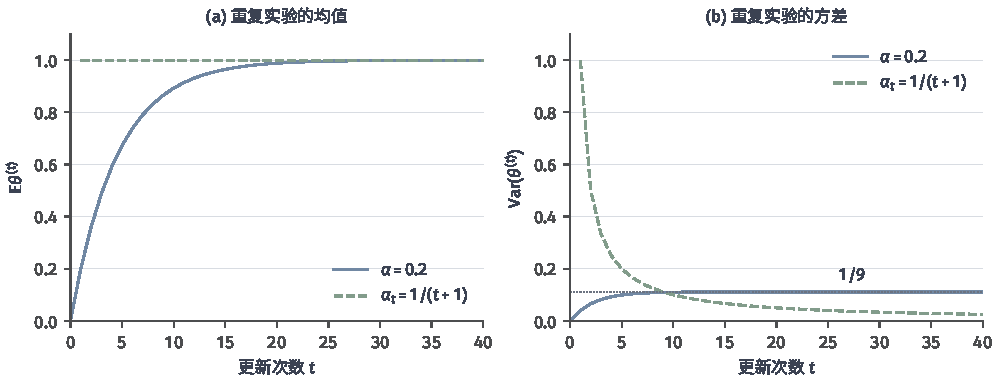
\includegraphics[width=\linewidth]{figures/00-shared/mathematical-preliminaries-lower/02-dynamical-systems-control-decision-and-games/matplotlib/stochastic-stepsize-bias-variance/figure.pdf}
  \caption{同一均值问题的重复实验均值与方差。取$\theta^{(0)}=0,\mu=1,\sigma^2=1$，
  观测独立同分布；蓝实线为固定$\alpha=0.2$，绿虚线为$\alpha_t=1/(t+1)$。
  固定步长方差趋于$1/9$，样本平均方差为$1/t$。曲线由解析式得到，不是一条样本轨迹。}
  \label{fig:stochastic-stepsize-bias-variance}
\end{figure*}

要把“噪声越来越小”变成逐路径收敛，需要控制累计噪声，而不只计算单步均值。
下面保留一个可完整证明的代表性结论。
\begin{lemma}[带可求和误差的非负超鞅]
  \label{lem:stoch-almost-supermartingale}
  设$Z_t,A_t$为关于$\mathcal F_t$的非负可积适应过程，$b_t\geq0$为确定数，
  且$\mathbb E[Z_{t+1}\mid\mathcal F_t]\leq Z_t-A_t+b_t$。
  若$\sum_tb_t<\infty$，则$Z_t$几乎必然收敛到有限随机变量，
  且$\sum_tA_t<\infty$几乎必然成立。
\end{lemma}
\begin{proof}
  令$r_t=\sum_{s=t}^\infty b_s$、$U_t=Z_t+r_t$。因为$r_t=b_t+r_{t+1}$，
  有$\mathbb E[U_{t+1}\mid\mathcal F_t]\leq U_t-A_t$。
  $U_t$是非负超鞅，由非负超鞅收敛定理几乎必然收敛到有限值。
  取期望并累加得到
  $\mathbb E\sum_{t=0}^nA_t\leq\mathbb E U_0$。
  单调收敛给出$\mathbb E\sum_{t=0}^\infty A_t\leq\mathbb E U_0<\infty$，
  所以该非负级数几乎必然有限。又$r_t\to0$，故$Z_t=U_t-r_t$也收敛。
\end{proof}
其中的鞅与超鞅收敛工具见第~\ref{chap:stochastic-processes-and-approximation}章；
本引理把可求和误差吸收到一个真正的超鞅中。

\begin{theorem}[均值求根的几乎必然收敛]
  \label{thm:stoch-mean-root-convergence}
  设$\mathcal F_t$包含$\theta^{(0)},Y_1,\ldots,Y_t$，且
  $\mathbb E[(\theta^{(0)}-\mu)^2]<\infty$。若
  \[
    \mathbb E[Y_{t+1}\mid\mathcal F_t]=\mu,\qquad
    \mathbb E[(Y_{t+1}-\mu)^2\mid\mathcal F_t]\leq\sigma^2,
  \]
  步长满足式~\eqref{eq:stoch-robbins-monro-stepsizes}并最终有$0<\alpha_t\leq1$，
  则式~\eqref{eq:stoch-robbins-monro-mean}的$\theta^{(t)}\to\mu$几乎必然成立。
\end{theorem}
\begin{proof}
  记$e_t=\theta^{(t)}-\mu$、$\xi_{t+1}=Y_{t+1}-\mu$，则
  $e_{t+1}=(1-\alpha_t)e_t+\alpha_t\xi_{t+1}$。
  初值与条件二阶矩假设递归保证每个有限时刻的$\mathbb E e_t^2$有限。
  舍去有限前缀，令$0<\alpha_t\leq1$。条件展开平方，交叉项为零，得到
  \[
    \mathbb E[e_{t+1}^2\mid\mathcal F_t]
    =(1-\alpha_t)^2e_t^2
      +\alpha_t^2\mathbb E[\xi_{t+1}^2\mid\mathcal F_t]
    \leq e_t^2-\alpha_te_t^2+\alpha_t^2\sigma^2.
  \]
  对移位序列应用前一引理，取$Z_t=e_t^2,A_t=\alpha_te_t^2$、
  $b_t=\alpha_t^2\sigma^2$。可积性与可求和条件均已核对，故$e_t^2$几乎必然
  收敛，且$\sum_t\alpha_te_t^2<\infty$。
  若某条样本路径的极限为$L>0$，最终就有$e_t^2\geq L/2$，
  从而$\sum_t\alpha_te_t^2\geq(L/2)\sum_t\alpha_t=\infty$，矛盾。
  所以$L=0$，得到结论。
\end{proof}
平方可和控制噪声，步长和发散排除残留误差。若条件均值有不可忽略偏差，
或条件方差失控，证明中的递推不等式就失去依据。向量非线性情形还须控制迭代
有界性，不能把标量结论仅通过换粗体符号推广。

一般漂移适合在与步长匹配的时钟上观察。定义算法时间
\begin{equation}
  \tau_0=0,\qquad \tau_t=\sum_{s=0}^{t-1}\alpha_s,
  \label{eq:stoch-algorithmic-time}
\end{equation}
并在相邻$(\tau_t,\bm\theta^{(t)})$之间线性插值为$\widehat{\bm\theta}(\tau)$。
对应平均ODE是
\begin{equation}
  \dot{\bm\theta}(\tau)=\overline{\bm h}(\bm\theta(\tau)).
  \label{eq:stoch-mean-ode}
\end{equation}
\term{ODE方法}不是说每个随机增量都等于平均增量，而是要求任意固定算法时间窗
上的累计随机偏差最终消失。要使插值轨迹在这些时间窗内跟随平均ODE，
可检查以下一组条件：$\alpha_t\to0$、
$\sum_t\alpha_t=\infty$，$\overline{\bm h}$局部Lipschitz，迭代几乎必然有界，
并对每个$H>0$有
\[
  \sup_{\substack{k\geq t\\\tau_k-\tau_t\leq H}}
  \left\|\sum_{s=t}^{k-1}\alpha_s(\bm\xi_{s+1}+\bm r_{s+1})\right\|
  \longrightarrow0\quad\text{几乎必然}.
\]
在这些条件下，插值的积分方程相对平均ODE只剩一个在有限窗上一致趋零的残差。
局部Lipschitz与有界性给出该窗口上的统一常数，应用
引理~\ref{lem:action-state-gronwall}，便得到插值与从同一晚期状态出发的ODE
轨迹在该窗上一致接近。这一步连接的是有限窗轨迹；再结合平均ODE的全局渐近
稳定平衡及紧集上的吸引性，才能得到迭代收敛到该平衡\scite{math-borkar2008stochastic}

对均值根，平均方程及其解为
\begin{equation}
  \dot\theta=\mu-\theta,\qquad
  \theta(\tau)=\mu+(\theta(0)-\mu)\mathrm e^{-\tau}.
  \label{eq:stoch-mean-root-ode-solution}
\end{equation}
取$V=(\theta-\mu)^2/2$则$\dot V=-(\theta-\mu)^2$，与前述误差平方证明一致。
一般系统可能有多个吸引子；平均稳定不意味着全局最优。迭代有界性也须证明，
例如建立远处负漂移的径向无界函数。投影到紧凸集虽可强制有界，却改变了边界上的
平均动力学；不能把所得极限不加论证地叫作原方程的根，或原根的欧氏投影。

现在转向相关观测。固定核$P$、平稳分布$\pi$，随机更新为$H(\theta,Z_t)$时，
平均漂移是
\begin{equation}
  \overline h(\theta)=\int H(\theta,z)\,\pi(\mathrm dz).
  \label{eq:stoch-markov-mean-field}
\end{equation}
即使$Z_t$已平稳，$H(\theta,Z_t)-\overline h(\theta)$给定过去也未必均值为零。
需要把相关误差转成可控制的鞅和边界项。
\begin{definition}[Markov核的Poisson方程]
  \label{def:stoch-markov-poisson-equation}
  固定$P,\pi$与$\pi$可积的$H(\theta,\cdot)$。若可测函数$g_\theta$满足
  \begin{equation}
    g_\theta(z)-Pg_\theta(z)=H(\theta,z)-\overline h(\theta),
    \qquad Pg_\theta(z)=\int g_\theta(z')P(z,\mathrm dz'),
    \label{eq:stoch-poisson-equation}
  \end{equation}
  且所用积分有限，则称其为相应\term{Poisson方程}的解。
\end{definition}
这个Poisson方程要求寻找一个函数，使它与一步转移后的平均之差等于中心化更新；其对象是Markov算子。第~\ref{sec:action-state-poisson-integral}节的Poisson计数过程记录事件到达，两者共用名称，执行的运算不同。
若链对历史满足$\mathcal L(Z_{t+1}\mid\mathcal F_t)=P(Z_t,\cdot)$，相关变量可积，
则
\begin{align}
  H(\theta,Z_t)-\overline h(\theta)
    &=g_\theta(Z_t)-g_\theta(Z_{t+1})+\Delta M_{t+1}(\theta),
       \label{eq:stoch-poisson-decomposition}\\
  \Delta M_{t+1}(\theta)&=g_\theta(Z_{t+1})-Pg_\theta(Z_t).\notag
\end{align}
最后一项给定$\mathcal F_t$均值为零；前两项固定参数时会望远镜消去。
参数与步长变化时还剩余项，不能直接把它们删掉。

\begin{lemma}[固定有限链的加权Poisson分解]
  \label{lem:stoch-finite-chain-poisson-sum}
  设$P$为固定的有限不可约非周期核，参数递推
  $\theta^{(t+1)}=\theta^{(t)}+\alpha_tH(\theta^{(t)},Z_t)$始终位于紧集$K$，
  $H$在$K$上一致有界且关于参数一致Lipschitz。若正步长单调递减并满足
  式~\eqref{eq:stoch-robbins-monro-stepsizes}，且链对所用历史具有上述条件转移核，
  则
  $\sum_{t=0}^n\alpha_t[H(\theta^{(t)},Z_t)-\overline h(\theta^{(t)})]$
  几乎必然收敛。特别地，任意向晚期移动的有限算法时间窗上的尾和趋零。
\end{lemma}
\begin{proof}
  记$q_\theta=H(\theta,\cdot)-\overline h(\theta)$。
  有限不可约非周期链几何收敛，且$\pi q_\theta=0$，所以
  $g_\theta=\sum_{j=0}^\infty P^jq_\theta$绝对一致收敛，并满足
  $g_\theta-Pg_\theta=q_\theta$。
  对$q_\theta-q_{\theta'}$应用相同几何界，得到有限常数$G,L_g$使
  $|g_\theta(z)|\leq G$、
  $|g_\theta(z)-g_{\theta'}(z)|\leq L_g|\theta-\theta'|$。

  加权鞅和$\sum_{t=0}^n\alpha_t\Delta M_{t+1}(\theta^{(t)})$的条件方差和被
  $4G^2\sum_t\alpha_t^2$控制，因而在$L^2$中有界并几乎必然收敛。
  剩余项从$m$到$n$作分部求和，得到
  \begin{align*}
    &\sum_{t=m}^n\alpha_t
       [g_{\theta^{(t)}}(Z_t)-g_{\theta^{(t)}}(Z_{t+1})]\\
    &\quad=\alpha_mg_{\theta^{(m)}}(Z_m)
       -\alpha_ng_{\theta^{(n)}}(Z_{n+1})\\
    &\qquad+\sum_{t=m+1}^n
       [\alpha_tg_{\theta^{(t)}}(Z_t)
        -\alpha_{t-1}g_{\theta^{(t-1)}}(Z_t)].
  \end{align*}
  中间每项绝对值至多
  $G(\alpha_{t-1}-\alpha_t)
    +\alpha_{t-1}L_g|\theta^{(t)}-\theta^{(t-1)}|$。
  有界更新给出$|\theta^{(t)}-\theta^{(t-1)}|\leq C\alpha_{t-1}$。
  第一部分由单调性望远镜求和，第二部分由平方可和控制，端点因$\alpha_t\to0$
  而消失。故剩余级数也收敛，与鞅和相加即得结论。收敛级数的任意尾区间和一致
  趋零，自然包含固定算法时间长度对应的索引窗。
\end{proof}

例~\ref{ex:stoch-two-state-chain}中的链取值$0,2$，平稳均值$\mu=2/3$，
且$P(z-\mu)=0.7(z-\mu)$。对$H(\theta,z)=z-\theta$，可取
$g_\theta(z)=(z-\mu)/(1-0.7)=\frac{10}{3}(z-\mu)$。
它恰好不依赖参数，因此参数变化余项也消失。Poisson分解没有把相关样本变成独立
样本，而是重新组织累计误差。

一般状态空间要另外证明Poisson解存在、具有所需矩界且随参数规则变化。
若$Z_{t+1}\sim P_{\bm\theta^{(t)}}(Z_t,\cdot)$，则平均漂移也变成
$\overline{\bm h}(\bm\theta)=\int\bm H(\bm\theta,z)\pi_{\bm\theta}(\mathrm dz)$，
相应方程为$g_{\bm\theta}-P_{\bm\theta}g_{\bm\theta}
=H(\bm\theta,\cdot)-\overline h(\bm\theta)$。
每个固定参数下分别遍历并不够：算法不断改变参数，需要在访问区域上统一控制
混合速度、Poisson解的矩及参数Lipschitz界，再控制参数变化造成的加权余项。
统一几何遍历、适当的矩界与联合有界性是常见充分条件。
它们使相关波动在算法时间上可忽略，不能把不稳定的平均根变成稳定根。

\paragraph{平均动力学的稳定条件}
\label{sec:dynamical-mean-dynamics-linear-recursion}

下面假定步长和噪声已经满足前述接口，只检查平均方向怎样消退变量误差。线性平均漂移
常写为
\begin{equation}
  \overline{\bm h}(\bm\theta)=\bm b-\bm A\bm\theta.
  \label{eq:dynamical-linear-mean-drift}
\end{equation}
若$\bm A$可逆，平衡为$\bm\theta^\star=\bm A^{-1}\bm b$，误差满足
\begin{equation}
  \dot{\bm e}=-\bm A\bm e.
  \label{eq:dynamical-linear-mean-error-ode}
\end{equation}
若\(-\bm A\)的全部特征值实部为负，就称\(-\bm A\)为Hurwitz矩阵；等价地，\(\bm A\)的特征值实部为正。这样的平均误差会指数消退，谱判据的证明见定理~\ref{thm:dynamical-continuous-spectral-stability}。
负号不可漏掉。$\bm A$也未必是某个损失的Hessian，不能仅凭更新外形套用凸性。

对一般实矩阵，反对称部分的二次型为零，因而
$\bm e^\top\bm A\bm e=\bm e^\top(\bm A+\bm A^\top)\bm e/2$。
若
\begin{equation}
  \frac{\bm A+\bm A^\top}{2}\succ\bm0,
  \label{eq:dynamical-positive-symmetric-part}
\end{equation}
则欧氏能量$V=\|\bm e\|_2^2/2$严格下降，给出方便的充分条件。
它不是必要条件：$\bm A=\left[\begin{smallmatrix}1&10\\0&1\end{smallmatrix}\right]$
的特征值均为$1$，而对称部分
$\left[\begin{smallmatrix}1&5\\5&1\end{smallmatrix}\right]$有负特征值。
平均误差仍指数稳定，只是欧氏范数可能暂时增大。只要$-\bm A$为Hurwitz矩阵，
定理~\ref{thm:dynamical-linear-lyapunov-equation}中的线性Lyapunov方程便为任意$\bm Q\succ\bm0$给出$\bm P\succ\bm0$满足
\begin{equation}
  \bm A^\top\bm P+\bm P\bm A=\bm Q.
  \label{eq:dynamical-mean-drift-lyapunov}
\end{equation}
此时$V=\bm e^\top\bm P\bm e$的导数为$-\bm e^\top\bm Q\bm e$，
所以$\bm P$所定义的二次误差在$\bm e\ne\bm0$时严格下降。
这说明欧氏误差可以暂时增大，而换用合适的正定二次型仍能证明误差衰减。

时序差分（temporal difference, TD）更新提供了一个具体来源。
固定只依赖当前状态的行动规则$\pi$后，设有限状态$S_t$按转移矩阵$\bm P_\pi$演化，
每步收益$R_{t+1}$按当前转移产生，其规律不随时间改变且绝对值有界。
取$0\leq\gamma<1$，从状态$i$出发的收益价值定义为
\[
 v_\pi(i)=\mathbb E_i^\pi
 \left[\sum_{k=0}^\infty\gamma^kR_{k+1}\right].
\]
这里近似的是累计收益的期望，不是某一次随机实现；
下标$i$表示把初态固定为$i$，几何级数保证这个期望有限。
拆出第一步，并按下一状态作条件平均，便有
\[
 v_\pi(i)=\mathbb E_i^\pi[R_1+\gamma v_\pi(S_1)].
\]
用特征$\bm\phi(i)\in\mathbb R^q$的线性组合$\bm\phi(i)^\top\bm\theta$近似$v_\pi(i)$，
再以样本转移$i\to j$及收益$R$替代这个条件平均，便得到更新方向
$\bm\phi(i)[R+\gamma\bm\phi(j)^\top\bm\theta-\bm\phi(i)^\top\bm\theta]$。
它用当前值与“一步收益加下一状态值”的差纠正参数。
令平稳访问概率为$\bm d$、$\bm D=\operatorname{diag}(\bm d)$，
$\bm\Phi$的第$i$行为$\bm\phi(i)^\top$，
在同一策略的平稳访问下平均得到
\begin{equation}
  \overline{\bm h}(\bm\theta)=\bm b-\bm A_{\mathrm{TD}}\bm\theta,\qquad
  \bm A_{\mathrm{TD}}=\bm\Phi^\top\bm D
                    (\bm I-\gamma\bm P_\pi)\bm\Phi.
  \label{eq:dynamical-td-mean-matrix}
\end{equation}
若$r_i=\mathbb E[R\mid i]$，则$\bm b=\bm\Phi^\top\bm D\bm r$。
固定策略的求值关系在这里解释非对称平均矩阵的来源，策略的选择则留给
\BookChapterRef{chap:policy-value-and-optimization}{第~\ref{chap:policy-value-and-optimization}章}。该章主要按成本计价，
把本例收益取负即可转换到相应的成本价值约定。

先设所考虑状态的$d_i>0$，以便
$\|\bm z\|_{\bm D}=(\bm z^\top\bm D\bm z)^{1/2}$为范数。
Jensen不等式给出$(\bm P_\pi\bm z)_i^2\leq\sum_j(P_\pi)_{i,j}z_j^2$；
乘$d_i$求和，并用平稳性$\sum_id_i(P_\pi)_{i,j}=d_j$，得到
\begin{equation}
  \|\bm P_\pi\bm z\|_{\bm D}\leq\|\bm z\|_{\bm D}.
  \label{eq:dynamical-markov-contraction-weighted}
\end{equation}
再由Cauchy--Schwarz，
$\langle\bm z,\bm P_\pi\bm z\rangle_{\bm D}\leq\|\bm z\|_{\bm D}^2$。
取$\bm z=\bm\Phi\bm c$，便有
\begin{align}
  \bm c^\top\bm A_{\mathrm{TD}}\bm c
    &=\|\bm\Phi\bm c\|_{\bm D}^2
       -\gamma\langle\bm\Phi\bm c,\bm P_\pi\bm\Phi\bm c\rangle_{\bm D}\notag\\
    &\geq(1-\gamma)\|\bm\Phi\bm c\|_{\bm D}^2.
    \label{eq:dynamical-td-positive-drift}
\end{align}
若$\bm\Phi^\top\bm D\bm\Phi\succ\bm0$，右侧对$\bm c\neq\bm0$严格为正，
所以平均矩阵的对称部分正定，具有唯一全局指数稳定平衡。
若允许$d_i=0$，加权量在全空间只是半范数，但上面的求和不等式仍成立；
严格结论仍须直接要求加权特征协方差正定，普通满列秩未必足够。
离策略采样改变访问权重而不同时改变目标转移，非扩张不等式可能失败，
故不能由此推出离策略稳定。

再用标量递推核对平均稳定与噪声条件怎样配合。设
$\theta^{(t+1)}=\theta^{(t)}+\alpha_t[b-a\theta^{(t)}+\xi_{t+1}]$，
$a>0$，噪声为条件均值零且条件二阶矩不超过$\sigma^2$，初值二阶矩有限。
令$e_t=\theta^{(t)}-b/a$，则
\[
  \mathbb E[e_{t+1}^2\mid\mathcal F_t]
  =(1-a\alpha_t)^2e_t^2+
       \alpha_t^2\mathbb E[\xi_{t+1}^2\mid\mathcal F_t].
\]
当$0<a\alpha_t\leq1$，右侧至多
$e_t^2-a\alpha_te_t^2+\alpha_t^2\sigma^2$。
应用已证几乎超鞅引理与两组步长级数，即得$e_t\to0$几乎必然；
在这个标量例中，论证本身给出路径有界性，无需额外假设。
固定步长另须$|1-a\alpha|<1$。若噪声独立同分布，具有正方差$v$并独立于初值，
由同一方差递推可得稳态误差方差
\[
 \frac{\alpha^2v}{1-(1-a\alpha)^2}>0.
\]
仅有条件二阶矩上界不能推出这一正方差结论，因为噪声也可能为零或逐渐减弱。

\subsection{双时间尺度下的迭代序列收敛}
\label{sec:action-state-two-timescale}

仍以未知均值$\mu$为例，我们可以用两个算法变量$u,v$分担估计，
使$u+v$接近$\mu$。给定当前的$v$，先让$u$较快地估计剩余部分$\mu-v$，
再让$v$较慢地调整，使两部分的估计趋于一致。
慢变量改变时，快变量的目标也随之改变；若二者的更新速度相差足够大，
就可以先分析近似固定$v$时$u$怎样跟踪，再分析$v$的变化。
后面的均值拆分例会把这两步具体算出。一般地，用两组步长写成
\begin{align*}
  \bm u^{(t+1)}
    &=\bm u^{(t)}+\beta_t[
        \bm g(\bm u^{(t)},\bm v^{(t)})+\bm\eta_{t+1}+\bm r^u_{t+1}],\\
  \bm v^{(t+1)}
    &=\bm v^{(t)}+\alpha_t[
        \bm f(\bm u^{(t)},\bm v^{(t)})+\bm\xi_{t+1}+\bm r^v_{t+1}].
\end{align*}
这里$\bm u^{(t)},\bm v^{(t)}$是算法变量，不是贯穿温度模型的行动与读数。
两组步长都满足Robbins--Monro条件，且$\alpha_t/\beta_t\to0$时，
$\bm u$相对较快，$\bm v$相对较慢。例如
$\beta_t=(t+1)^{-0.6}$、$\alpha_t=(t+1)^{-0.9}$满足尺度分离。

快时间上把$\bm v$暂时固定，得到
$\dot{\bm u}=\bm g(\bm u,\bm v)$；若其稳定平衡为$\bm u^\star(\bm v)$，
慢时间上再使用
$\dot{\bm v}=\bm f(\bm u^\star(\bm v),\bm v)$。
一组常用的充分条件是：漂移局部Lipschitz；快平衡对每个慢状态全局渐近稳定，
其吸引性在所访问的紧参数区域上一致，且平衡映射局部Lipschitz；约化慢ODE有
全局渐近稳定平衡$\bm v^\star$；联合迭代几乎必然有界；两组鞅差的条件二阶矩
在访问区域有统一界，残差在各自有限算法时间窗上可忽略。在这些条件与步长条件下，
标准双时间尺度结论给出
$(\bm u^{(t)},\bm v^{(t)})\to
(\bm u^\star(\bm v^\star),\bm v^\star)$\scite{math-borkar2008stochastic}
Markov背景则需在两个时钟上分别验证相应的Poisson与统一混合条件。

\begin{example}[分解同一个未知均值的快慢更新]
  \label{ex:stoch-two-timescale-mean-splitting}
  若$\mathbb E[Y_{t+1}\mid\mathcal F_t]=\mu$，取
  \[
    u^{(t+1)}=u^{(t)}+\beta_t(Y_{t+1}-u^{(t)}-v^{(t)}),\qquad
    v^{(t+1)}=v^{(t)}+\alpha_t(u^{(t)}-v^{(t)}).
  \]
  冻结$v$后，快方程$\dot u=\mu-v-u$的唯一稳定平衡为$u^\star(v)=\mu-v$。
  代入慢方程得$\dot v=\mu-2v$，于是$v^\star=\mu/2$，
  $u^\star(v^\star)=\mu/2$。快变量估计尚未被$v$解释的部分，慢变量调整两部分
  的分配。若再满足两组步长条件、统一有界的条件噪声方差、有限二阶矩初值以及
  联合迭代几乎必然有界，则上述条件给出联合收敛。
\end{example}
尺度分离没有保证快平衡存在，也没有保证其稳定或全局最优。两组步长同阶时，
前面的均值拆分例仍可用联合系统分析，却不能继续使用冻结慢变量的论证。
两类极限还可以由噪声尺度区分。这里的噪声增量是$\alpha_t\xi_{t+1}$，方差尺度为$\alpha_t^2$；式~\eqref{eq:dynamical-euler-maruyama}的扩散模拟使用$\sqrt h\,\xi$，方差尺度为$h$。
平均ODE中噪声在有限算法时间窗消失，SDE中噪声则保留有限二次变差，两者不能互换。

\subsection{长时间采样下的分布与平均收敛}
给定一张难以直接采样的目标分布，可以反过来设计一条随机演化规律，使得系统无论从什么初态出发，长时间运行后其状态分布都会收敛到这张目标分布；于是只要把这条链跑得足够久、并记下沿途状态，就得到了可用于数值积分的（相关）样本，这正是 Langevin 动力学、HMC 等采样方法的基本思想。需要检查两步：目标是否被演化保持（从目标出发不会离开），以及从实际初态出发能否接近它（混合）。第~\ref{sec:stoch-markov-long-run-average}节已经区分时间平均与逐时刻分布的极限；这里还要加入数值离散对目标的影响。

设目标密度$\pi>0$光滑且可归一化。过阻尼Langevin模型为
\begin{equation}
 \mathrm d\bm X_t=\tfrac12\nabla\log\pi(\bm X_t)\,\mathrm dt+\mathrm d\bm W_t.
 \label{eq:dynamical-langevin-sde}
\end{equation}
代入Fokker--Planck通量，$\bm b\pi-\nabla\pi/2=\bm0$。
在方程无爆炸、边界通量为零及密度方程适定等条件下，这证明$\pi$不变。
从其他初态收敛还需遍历条件；例如$\pi\propto\mathrm e^{-U}$，
$U$光滑强凸且梯度全局Lipschitz时，噪声非退化与向内漂移提供常用保证。
多峰势能可能保持同一目标却混合很慢。

即使连续模型正确，离散化也会改变稳态。取$\pi=\mathcal N(0,1)$，
则$X_{k+1}=(1-h/2)X_k+\sqrt h\,\varepsilon_k$。
只有$0<h<4$时这一递推稳定，其稳态方差为
\[
  \frac{h}{1-(1-h/2)^2}=\frac1{1-h/4},
\]
并非$1$。减小步长减小偏差，但在相同计算步数下也缩短模拟时间；
有限预算须同时考虑初态遗留、相关性和离散误差。

Hamilton蒙特卡洛（HMC）使用另一种构造。若
$\pi(\bm q)\propto\exp[-U(\bm q)]$，引入独立
$\bm p\sim\mathcal N(\bm0,\bm M)$，联合密度为
$\rho(\bm q,\bm p)\propto\exp[-H(\bm q,\bm p)]$。
精确Hamilton流保持能量和体积，因此保持$\rho$；
蛙跳只保持体积与可逆结构，需要接受校正补偿能量误差。
固定步长$h$与步数$L$，记$T=R\circ\Psi_h^L$，
其中$R(\bm q,\bm p)=(\bm q,-\bm p)$。
前面已证明$R\Psi_hR=\Psi_h^{-1}$，故$T^2=I$，且$|\det DT|=1$。
对$\bm z' =T\bm z$，接受概率取
\begin{equation}
 \alpha(\bm z)=\min\{1,\exp[-H(\bm z')+H(\bm z)]\}.
 \label{eq:dynamical-hmc-acceptance}
\end{equation}

\begin{theorem}[HMC提议的细致平衡]
 \label{thm:action-state-hmc-balance}
 若$T$是可微、体积保持的对合，则以概率$\alpha(\bm z)$移至$T\bm z$，
 否则留在$\bm z$的核，对密度$\rho$满足细致平衡。
\end{theorem}
\begin{proof}
 接受部分的密度权重为
 $\rho(\bm z)\alpha(\bm z)=\min\{\rho(\bm z),\rho(T\bm z)\}$。
 对任意有界可测函数$g(\bm z,\bm z')$，作变量替换$\bm y=T\bm z$，
 由$T^2=I$和单位绝对Jacobian，
 \[
 \begin{split}
 &\int g(\bm z,T\bm z)\min\{\rho(\bm z),\rho(T\bm z)\}\,\mathrm d\bm z\\
 &\quad=\int g(T\bm y,\bm y)
                   \min\{\rho(T\bm y),\rho(\bm y)\}\,\mathrm d\bm y .
 \end{split}
 \]
 这证明接受部分在交换出发与到达状态后不变。
 拒绝部分集中在对角线$\bm z'=\bm z$，本身对称，两者相加即为细致平衡。
\end{proof}

一轮算法因而是：保留当前位置并重新抽取高斯动量；按三子步蛙跳执行$L$次；
翻转末端动量并计算$\Delta H$；抽取独立均匀数，按
$\min(1,\mathrm e^{-\Delta H})$接受，否则保留原位置。
动量刷新是联合目标的条件抽样，保持$\rho$；再接上述核仍保持$\rho$，
边缘化动量得到位置目标$\pi$。两个保持核的复合不必在联合空间仍可逆，
此处不把复合的不变性误说成自动细致平衡。

若提议不保持体积，接受比还需Jacobian因子；状态依赖地改变步数或步长，
也须重新核对反向提议。实现中的有限精度可逆误差不是上述精确算术证明的一部分。
接受校正不保证独立样本或快速混合：步长过大导致拒绝，轨迹过短导致高相关，
质量矩阵失配使不同方向移动不均衡。采样以保持分布为目标，不要求能量一路下降，
所以不能将Hamilton轨迹解释为更快的梯度下降。

\begin{table*}[htbp]
 \centering
 \begin{tabularx}{\linewidth}{lXX}
 \toprule
 结论 & 所比较的对象 & 尚未得到的保证\\
 \midrule
 强数值误差小 & 同一驱动下数值状态与真状态 & 长期抽样偏差小\\
 弱数值误差小 & 两种状态分布的测试函数期望 & 单条路径距离小\\
 密度$\pi$不变 & 从$\pi$出发仍保持$\pi$ & 其他初态快速趋于$\pi$\\
 概率流匹配边缘 & 每个时刻的状态分布 & 相同时间间联合规律\\
 \bottomrule
 \end{tabularx}
 \caption{随机演化中几种保证的对象。每一项均依赖相应段落给出的正则、边界或数值条件，
 不能用一个对象上的结论替代另一个对象上的结论。}
 \label{tab:dynamical-path-distribution}
\end{table*}

\section{状态演化的扰动与稳定性}
\label{sec:dynamical-stability-sensitivity}
收敛结论说明轨迹的极限，扰动分析则固定一组演化规律，比较改变初值或输入后的轨迹。需要区分有限时间内误差可控、全部未来误差始终小，以及误差逐渐消退。线性谱与Lyapunov函数分别利用传播结构和标量下降关系给出判据。

\subsection{初值扰动下的轨迹稳定性}
前述原点判据通常对应零输入，或把恒定输入下的平衡平移到原点。
温度例的恒定$u_t=0.4$对应平衡$2$，误差$e_t=x_t-2$才满足$e_{t+1}=0.8e_t$。
不能因为误差趋零，就说实际温度趋于环境温度。

对连续方程，若$\bm f$关于状态具有Lipschitz常数$L$，同一输入下两条解满足
\[
  \|\bm x(t)-\widetilde{\bm x}(t)\|
  \leq \mathrm e^{L(t-t_0)}\|\bm x_0-\widetilde{\bm x}_0\|.
\]
积分方程与引理~\ref{lem:action-state-gronwall}给出这个有限时间连续依赖界。它允许误差随时间增长，尚未说明系统会消退初值差异。要得到衰减，须利用演化方向，而非只限制变化率；线性传播和Lyapunov下降关系分别提供这样的判据。

\subsubsection{线性演化下的轨迹稳定性}
\paragraph{长期演化的谱判据}

离散齐次系统为
\begin{equation}
  \bm x_{t+1}=\bm A\bm x_t,\qquad \bm x_t=\bm A^t\bm x_0.
  \label{eq:dynamical-discrete-linear-homogeneous}
\end{equation}
这里用矩阵幂和Jordan分解把长期轨迹问题化成谱的位置；下面对各Jordan块的幂
逐项给出长期估计。
\begin{theorem}[离散线性系统的渐近稳定性]
  \label{thm:dynamical-discrete-spectral-stability}
  式~\eqref{eq:dynamical-discrete-linear-homogeneous}的原点全局渐近稳定，
  当且仅当$\rho(\bm A)=\max_{\lambda\in\operatorname{spec}(\bm A)}|\lambda|<1$。
  在此条件下，原点实际上全局指数稳定。
\end{theorem}
\begin{proof}
  在复数域写$\bm A=\bm V\bm J\bm V^{-1}$。大小为$r$的Jordan块
  $\bm J_\lambda=\lambda\bm I+\bm N$满足
  \[
    \bm J_\lambda^t
      =\sum_{j=0}^{\min(t,r-1)}\binom tj\lambda^{t-j}\bm N^j.
  \]
  $\lambda=0$的块在有限步后为零；$0<|\lambda|<1$时，多项式因子被几何衰减
  压过。取$\rho(\bm A)<q<1$，全部有限个块可统一控制为$Cq^t$，乘回换基矩阵
  得$\|\bm A^t\|\leq C' q^t$。它既给出趋零，也给出稳定性所需的统一有界增益。
  反之，若存在$|\lambda|\geq1$，沿其特征向量的复轨迹不趋零；分解成实部与虚部，
  至少一条实轨迹不趋零。单位模特征值的非平凡Jordan块还可能多项式增长。
  故渐近稳定要求全部特征值严格在单位圆内。
\end{proof}

\begin{theorem}[连续线性系统的指数稳定性]
  \label{thm:dynamical-continuous-spectral-stability}
  系统$\dot{\bm x}=\bm A\bm x$的原点全局指数稳定，当且仅当$\bm A$的全部
  特征值实部严格为负。这样的矩阵称为Hurwitz矩阵。
\end{theorem}
\begin{proof}
  对Jordan块，
  $\mathrm e^{t(\lambda\bm I+\bm N)}
   =\mathrm e^{\lambda t}\sum_{j=0}^{r-1}t^j\bm N^j/j!$。
  若全部实部为负，取$0<\alpha<-\max_\lambda\operatorname{Re}\lambda$，
  有限次多项式乘指数可统一控制为$C\mathrm e^{-\alpha t}$。乘回换基矩阵就得到
  $\|\mathrm e^{t\bm A}\|\leq C'\mathrm e^{-\alpha t}$。
  若某个特征值实部非负，则对应实不变子空间中存在增长、常值或不衰减振荡的轨迹，
  不可能满足该指数界。非平凡Jordan块不会消除这种障碍。
\end{proof}
连续系统检查左半平面，离散系统检查单位圆。边界上的谱需另查Jordan结构：
可能稳定而不吸引，也可能增长，不能把严格不等号改成非严格不等号。

谱给出长期方向，二次能量给出一个可逐时刻检查的证书。取
$V(\bm x)=\bm x^\top\bm P\bm x$，其中$\bm P\succ\bm0$，则
\begin{equation}
  \dot V=\bm x^\top(\bm A^\top\bm P+\bm P\bm A)\bm x.
  \label{eq:dynamical-continuous-lyapunov-derivative}
\end{equation}
\begin{theorem}[线性Lyapunov方程]
  \label{thm:dynamical-linear-lyapunov-equation}
  $\bm A$为Hurwitz矩阵，当且仅当对每个$\bm Q\succ\bm0$，存在唯一
  $\bm P\succ\bm0$满足
  \begin{equation}
    \bm A^\top\bm P+\bm P\bm A=-\bm Q.
    \label{eq:dynamical-continuous-lyapunov-equation}
  \end{equation}
\end{theorem}
\begin{proof}
  若$\bm A$为Hurwitz矩阵，定义
  $\bm P=\int_0^\infty\mathrm e^{t\bm A^\top}\bm Q\mathrm e^{t\bm A}\,\mathrm dt$。
  指数稳定保证积分收敛。任意非零$\bm x$对应的被积二次型非负，且在$t=0$
  严格为正，所以$\bm P\succ\bm0$。对被积矩阵求导并积分，得
  \[
    \bm A^\top\bm P+\bm P\bm A
    =[\mathrm e^{t\bm A^\top}\bm Q\mathrm e^{t\bm A}]_0^\infty=-\bm Q.
  \]
  两解之差$\bm D$满足$\bm A^\top\bm D+\bm D\bm A=\bm0$，故
  $\mathrm e^{t\bm A^\top}\bm D\mathrm e^{t\bm A}$恒为$\bm D$；
  令$t\to\infty$得$\bm D=\bm0$。

  反之，若存在正定的$\bm P,\bm Q$满足方程，记
  $p_-=\lambda_{\min}(\bm P)$、$p_+=\lambda_{\max}(\bm P)$、
  $q_-=\lambda_{\min}(\bm Q)$。则
  $p_-\|\bm x\|_2^2\leq V\leq p_+\|\bm x\|_2^2$，且
  $\dot V=-\bm x^\top\bm Q\bm x\leq-(q_-/p_+)V$。
  乘以积分因子得到
  \[
    \|\bm x(t)\|_2
    \leq\sqrt{p_+/p_-}\,
      \mathrm e^{-q_-t/(2p_+)}\|\bm x(0)\|_2.
  \]
  这直接证明指数稳定；由已证谱判据，$\bm A$为Hurwitz矩阵。
\end{proof}
反向证明只用二次型上下界与积分估计，不依赖尚未建立的非线性判据。

这个方程在小尺寸下可以手算。取
\(\bm A=\begin{bmatrix}0&1\\-2&-3\end{bmatrix}\)，特征值为\(-1,-2\)，
都在左半平面。令\(\bm Q=\bm I\)并假定\(\bm P\)对称，写出
\(\bm P=\begin{bmatrix}p&q\\q&r\end{bmatrix}\)，
方程给出三个标量等式\(-4q=-1\)、\(p-3q-2r=0\)、\(2q-6r=-1\)，
解得\(q=1/4\)、\(r=1/4\)、\(p=5/4\)。
由此得到的\(\bm P\)特征值约为\(1.309\)与\(0.191\)，都为正，
验证了\(\bm P\succ\bm0\)。这个二次型也给出了收敛速度的估计：
\(q_-=1\)、\(p_+\approx1.309\)，衰减率约为\(1/(2\times1.309)\approx0.38\)，
即该范数衰减上界的时间常数约为\(2.6\)：经过这段时间，上界乘以\(e^{-1}\)。若以减半计，相应时间约为\(\log 2/0.38\approx1.8\)。这是一项由Lyapunov估计得到的保证，不是精确的最慢模态衰减率。
换一个\(\bm Q\)会得到不同的\(\bm P\)，但同一\(\bm A\)的稳定性结论不变。

\begin{theorem}[离散时间Lyapunov方程]
  \label{thm:dynamical-discrete-lyapunov-equation}
  $\rho(\bm A)<1$，当且仅当对每个$\bm Q\succ\bm0$，存在唯一
  $\bm P\succ\bm0$满足$\bm A^\top\bm P\bm A-\bm P=-\bm Q$。
\end{theorem}
\begin{proof}
  正向取
  $\bm P=\sum_{j=0}^\infty(\bm A^\top)^j\bm Q\bm A^j$。
  上述离散指数界使级数绝对收敛；首项正定、其余项半正定，故$\bm P$正定。
  左乘$\bm A^\top$、右乘$\bm A$后相减即得方程。两解之差满足
  $\bm D=(\bm A^\top)^t\bm D\bm A^t$，令$t\to\infty$得唯一性。
  反向用$V(\bm x)=\bm x^\top\bm P\bm x$，有
  \[
    V(\bm A\bm x)-V(\bm x)=-\bm x^\top\bm Q\bm x<0
    \quad(\bm x\neq\bm0).
  \]
  比值$V(\bm A\bm x)/V(\bm x)$在单位球面上连续且严格小于$1$，
  因紧性有统一上界$c<1$，且$c\geq0$。于是$V(\bm x_t)\leq c^t V(\bm x_0)$
  （$c=0$时一步后即为零）。二次型界给出指数稳定，再由谱判据得到$\rho(\bm A)<1$。
\end{proof}
线性系统因此总能为稳定动力学找到某个二次能量，但这个能量一般不是欧氏范数平方。
下一项正说明更换度量为什么重要。

\paragraph{有限时间的瞬态放大}

取
\[
  \bm A=\begin{bmatrix}1/2&K\\0&1/2\end{bmatrix},\qquad K>0.
\]
无论$K$多大，谱半径均为$1/2$，而
\[
  \bm A^t=
  \begin{bmatrix}
    2^{-t}&tK\,2^{-(t-1)}\\0&2^{-t}
  \end{bmatrix}.
\]
从$\bm x_0=(0,1)^\top$出发，第一步即为$(K,1/2)^\top$，欧氏范数可以大幅
增长；之后$t2^{-t}\to0$才使状态趋零。这里放大来自第二坐标向第一坐标的耦合，
没有任何输入或数值误差。

\begin{figure}[htbp]
  \centering
  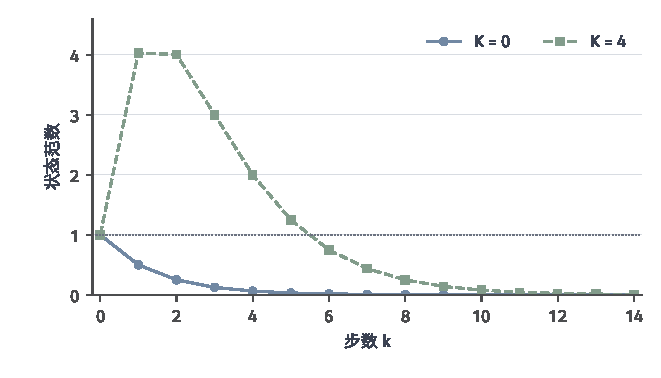
\includegraphics[width=\linewidth]{figures/00-shared/mathematical-preliminaries-lower/02-dynamical-systems-control-decision-and-games/matplotlib/dynamical-transient-growth/figure.pdf}
  \caption{同谱系统的不同瞬态。初值均为$(0,1)^\top$，蓝色圆点取$K=0$，
  绿色方点取$K=4$，谱半径均为$1/2$。后者前两步范数约为$4.03$、$4.01$，
  随后才趋零；灰线为初始范数$1$。长期衰减不等于每一步都收缩。}
  \label{fig:dynamical-transient-growth}
\end{figure}

$K\neq0$时，$\bm A^\top\bm A\neq\bm A\bm A^\top$，矩阵非正规。
本例只有一个独立特征向量，幂零耦合产生$t2^{-t}$项；可对角化但特征向量近乎
共线的非正规矩阵，也可能因模态先相消、后分离而放大。有限时间增益
$\|\bm A^t\|$与合适的Lyapunov范数描述了谱半径以外的信息。
还可考察允许小矩阵扰动时特征值能移动到哪里：在同维复矩阵上选定范数后，所有$\|\bm E\|<\varepsilon$对应的$\bm A+\bm E$的特征值并集称为$\varepsilon$伪谱。它反映谱对扰动的敏感性，与原矩阵的特征值集合不同。
谱稳定没有许诺欧氏范数下逐步收缩，更没有许诺中间状态不越过任务边界。

\subsubsection{非线性演化下的轨迹稳定性}
\label{sec:action-state-nonlinear-stability}
非线性系统一般无法通过一个固定矩阵构造全局二次能量，因而需要寻找候选函数。
它可以来自物理能量、误差平方或模型特有的守恒与耗散关系。找到候选以后，
仍须检查正定性、沿轨迹导数以及适用区域\scite{math-khalil2002nonlinear}
\begin{theorem}[连续时间Lyapunov判据]
  \label{thm:dynamical-nonlinear-lyapunov}
  设原点为$\dot{\bm x}=\bm f(\bm x)$的平衡点，$\bm f$在其邻域内局部Lipschitz。
  若该邻域存在$C^1$正定候选$V$且$\dot V\leq0$，则原点稳定；
  若非零点上$\dot V<0$，则原点局部渐近稳定。
  若这些条件在$\mathbb R^d$上成立，且$V(\bm x)\to\infty$当
  $\|\bm x\|\to\infty$，则所有解正向全局存在；非增情形给出稳定性，
  严格下降情形给出全局渐近稳定性。
\end{theorem}
\begin{proof}
  选足够小的$\varepsilon$使闭球位于适用邻域。球面上的连续正函数$V$有
  最小值$c_\varepsilon>0$。原点处连续性给出$\delta<\varepsilon$，
  使$\|\bm x_0\|<\delta$时$V(\bm x_0)<c_\varepsilon$。
  轨迹若首次触及球面，必须达到至少$c_\varepsilon$的能量，与$\dot V\leq0$
  矛盾。更具体地，可选$\bm x_0$所在的闭子水平集与闭球的交作为紧集$K$，
  且其能量水平严格低于球面最小值；轨迹不能穿出$K$，局部解可延拓到任意正时间。
  对全部足够小$\varepsilon$得到此结论即为稳定性。

  若$\dot V$在非零点严格为负，反设某条上述轨迹不趋零，则存在$\varepsilon_0>0$
  及$t_j\to\infty$，使$\|\bm x(t_j)\|\geq\varepsilon_0$。
  在紧集$K$上令$M=\sup_K\|\bm f\|$。非零轨迹下可取$M>0$；
  速度有界使每次达到该半径后至少在长度$\varepsilon_0/(2M)$内保持
  $\|\bm x\|\geq\varepsilon_0/2$。函数$-\dot V$在
  $K\cap\{\|\bm x\|\geq\varepsilon_0/2\}$上有严格正下界。
  选取互不相交的这些时间段，能量便减少无穷大量，与$V\geq0$矛盾。
  因而轨迹趋零。全局且径向无界时，每个初值的子水平集都紧；
  同样的延拓与下降论证适用于任意初值，得到全局结论。
\end{proof}
径向无界性控制的是远处状态，不能用“在原点附近正定”代替。
若还能找到$c_1,c_2,c_3>0$使
$c_1\|\bm x\|^2\leq V\leq c_2\|\bm x\|^2$、$\dot V\leq-c_3\|\bm x\|^2$，
则前述线性方程证明中的积分估计同样给出局部指数衰减。一般严格负导数未必有
这种二次型比较，所以渐近稳定未必指数稳定。

\subsection{输入扰动下的轨迹稳定性}
初值误差只在开始时注入，输入误差可以在每个时刻持续进入。即使无输入偏差会衰减，持续加热偏多仍可能造成非零温差。因此输入响应界需要把每个时刻的误差按剩余传播时间累计。

\subsubsection{线性演化下的轨迹响应}
对指数稳定线性系统，若
$\|\mathrm e^{t\bm A}\|\leq M\mathrm e^{-\alpha t}$，常数变易公式给出更强的界：
\[
  \|\bm x(t)\|
  \leq M\mathrm e^{-\alpha(t-t_0)}\|\bm x_0\|
  +M\|\bm B\|\int_{t_0}^t\mathrm e^{-\alpha(t-s)}\|\bm u(s)\|\,\mathrm ds.
\]
两组初值与输入之差仍满足同一个线性方程，因而把上式的$\bm x,\bm x_0,\bm u$分别换成状态差、初值差和输入差，就得到两条轨迹的比较界。若$\|\bm u(s)\|\leq U$，第二项至多
$(M\|\bm B\|U/\alpha)(1-\mathrm e^{-\alpha(t-t_0)})$。
有界输入产生有界状态，但持续输入通常留下非零稳态。
离散温度例若输入固定偏多$\delta u$，稳态偏差就是
$\delta u/(1-0.8)=5\delta u$。稳定性消退初值记忆，不会自动消除持续施加的偏差。

\subsubsection{非线性演化下的轨迹响应}
在初值连续依赖的基础上，再允许输入与向量场改变。设两条轨迹都留在同一区域，原向量场关于状态的Lipschitz常数为$L$，关于输入的常数为$L_u$；比较模型沿第二条轨迹的向量场误差至多为$r(s)$。Gronwall引理将初值误差、持续输入误差和模型误差合在同一传播界中：
\[
  \|\bm x(t)-\widetilde{\bm x}(t)\|
  \leq \mathrm e^{L(t-t_0)}\|\bm x_0-\widetilde{\bm x}_0\|
  +\int_{t_0}^t\mathrm e^{L(t-s)}
     \bigl(L_u\|\bm u(s)-\widetilde{\bm u}(s)\|+r(s)\bigr)\,\mathrm ds.
\]
初态误差、输入误差、模型误差因此有不同来源，却都要经过后续动态传播。

\section{基于观测的状态推断}
\label{sec:dynamical-state-space-filtering}
\label{sec:dynamical-stochastic-state-observation}

过程噪声规定真实状态如何随机移动；但真实状态往往无法直接读取，只能通过带误差的传感器间接观测——温度计有读数误差、雷达只能测距离而测不到完整位置。于是出现一个反向问题：给定一串传感器读数，怎样反推产生它们的隐藏状态轨迹？
因此推断不是再次生成一条任意轨迹，而是在已给定的生成模型中，保留与读数相容的
状态并重新分配概率：读数支持哪些状态，就提高它们的可能性，排除与之矛盾的状态。先明确已取得的传感器读数与所求状态量，再把预测、滤波和平滑化为可计算公式。

\subsection{观测条件下的推断目标}
在前面的状态转移$K_t$之外增加观测核
$G_t(\bm x,B)=\mathbb P(\bm y_t\in B\mid\bm x_t=\bm x)$。
它表示状态为$\bm x$时传感器返回哪些读数。线性加性例为
\begin{equation}
  \bm y_t=\bm C_t\bm x_t+\bm v_t.
  \label{eq:dynamical-linear-observation-model}
\end{equation}
先假设初值、所有过程噪声与所有观测噪声相互独立，输入与矩阵给定。
于是给定$\bm x_t$后，$\bm y_t$不再依赖旧状态和旧观测；
给定当前状态后，下一状态由$K_t$生成。联合规律在
式~\eqref{eq:dynamical-linear-state-model}的基础上分解为
\[
 \pi_0(\mathrm d\bm x_0)
       \prod_{t=0}^{T-1}K_t(\bm x_t,\mathrm d\bm x_{t+1})
       \prod_{t=1}^T G_t(\bm x_t,\mathrm d\bm y_t).
\]
这里从$y_1$开始观察，$\pi_0$不含一个未声明的$y_0$。
若噪声相关、传感器依赖旧状态或有内部滞后，须扩充联合状态或显式改写这些
条件关系。观测序列通常不满足自身的Markov性，因为一次带噪读数未必概括隐藏状态。

记$\mathcal Y_t=\sigma(\bm y_1,\ldots,\bm y_t)$，
$\mathcal Y_0$为无观测信息。欧氏状态与观测具有正则条件分布，
使“给定这段读数的状态概率”能作为概率核处理。
即使观测无噪，也不一定足够：$y_t=x_{1,t}+x_{2,t}$不能区分
$(1,0)^\top$与$(0,1)^\top$。能否借后续动力学区分这些方向，需要
\BookChapterRef{chap:control-theory}{第~\ref{chap:control-theory}章}的可观测性与可检测性条件。

这里“借后续动力学区分”可以算一遍。在一个无噪教学例中，设时刻$1$的状态
$\bm x_1$有$(1,0)^\top$或$(0,1)^\top$两个候选。
读数$y_1=x_{1,1}+x_{2,1}$对它们都等于$1$，仅凭它无法判断分量如何分配。
若动力学为$\bm x_{t+1}=\bm A\bm x_t+\bm u_t$，其中
$\bm A=\operatorname{diag}(0.5,2)$，在读得$y_1$之后施加共同已知输入
$\bm u_1=(0.5,0)^\top$，则时刻$2$的两个候选分别为
\[
 \bm A(1,0)^\top+\bm u_1=(1,0)^\top,\qquad
 \bm A(0,1)^\top+\bm u_1=(0.5,2)^\top.
\]
因此下一次读数$y_2=x_{1,2}+x_{2,2}$分别为$1$与$2.5$，两者便被分开。
共同输入在两个候选的状态差中相互抵消；区别来自状态转移把原先看不到的分量差
带入下一次读数。这个例子说明可观测性要连同状态转移
一起判断：一次观测丢掉的信息，可能被后续演化重新带到观测方向，也可能始终留在
看不到的子空间里。

\begin{example}[带泄漏温度的间接观测]
 \label{ex:dynamical-noisy-temperature}
 回到同一模型
 $x_{t+1}=0.8x_t+u_t+w_{t+1}$、$y_t=x_t+v_t$，
 其中$w_t\sim\mathcal N(0,0.04)$、$v_t\sim\mathcal N(0,0.09)$，
 与初值及彼此独立。即使传感器完全精确，未来仍因$w_{t+1}$不确定；
 即使过程无噪，当前状态也可能因读数噪声而不确定。
 图~\ref{fig:action-state-temperature-layers}的轨迹从已知$x_0=0$出发，
 使用给定$u_t=0.4$；后面的估计继续使用该初值与同一组读数，
 不另换一条更利于展示的状态轨迹。
\end{example}

得到条件分布后，还须规定输出什么估计。平方损失下，若$\bm X$二阶可积，
对信息$\mathcal G$可测的估计$\bm a$，
\[
 \mathbb E[\|\bm X-\bm a\|^2\mid\mathcal G]
 =\mathbb E[\|\bm X-\mathbb E(\bm X\mid\mathcal G)\|^2\mid\mathcal G]
       +\|\mathbb E(\bm X\mid\mathcal G)-\bm a\|^2.
\]
交叉项因条件均值为零而消失，所以条件均值最小化均方损失。
离散状态的零一损失选条件众数；连续密度的MAP是另一种点输出，
不能不说明损失就把所有“最优估计”视为同义。

\label{sec:dynamical-kalman-rts}

同一时刻的状态可以由不同范围的记录推断。只用此前记录、加入当前读数，或再加入事后读数，分别给出预测、滤波和平滑；所问物理状态没有改变，改变的是条件信息。固定目标时刻$t$，用$j$表示最后可见的观测时刻，并记
$\bm m_{t\mid j}=\mathbb E[\bm x_t\mid\mathcal Y_j]$、
$\bm P_{t\mid j}=\operatorname{Cov}(\bm x_t\mid\mathcal Y_j)$。
三种查询的区别先由信息范围决定，与使用哪一种算法无关。

\begin{table}[htbp]
 \centering
 \begin{tabularx}{\linewidth}{lXX}
 \toprule
 查询 & 目标条件分布 & 允许的观测\\
 \midrule
 一步预测 & $P(\bm x_t\mid\mathcal Y_{t-1})$ & 新读数以前\\
 当前滤波 & $P(\bm x_t\mid\mathcal Y_t)$ & 包括当前读数\\
 固定区间平滑 & $P(\bm x_t\mid\mathcal Y_T)$，$T>t$ & 包括事后未来读数\\
 \bottomrule
 \end{tabularx}
 \caption{同一目标状态的三种边缘查询。信息终点改变，物理状态并未改变；
 平滑使用的未来读数不能用于当时的在线行动。}
 \label{tab:dynamical-estimation-information}
\end{table}

下面的一般核公式只要求前述条件独立结构。需要解析闭合时，再采用有限时域
线性高斯条件：
\[
 \bm x_0\sim\mathcal N(\bm m_{0\mid0},\bm P_{0\mid0}),\quad
 \bm w_{t+1}\sim\mathcal N(\bm0,\bm Q_{t+1}),\quad
 \bm v_t\sim\mathcal N(\bm0,\bm R_t).
\]
三组随机量彼此独立，系统矩阵与输入确定，
$\bm P_{0\mid0},\bm Q_{t+1}\succeq\bm0$，先取$\bm R_t\succ\bm0$。
本章统一让$w_{t+1}$与它推动到达的状态时刻一致；
因此从$t-1$到$t$的过程协方差写为$\bm Q_t$。
这些条件在每个有限$T$内使用，不预设滤波增益已达稳态。

\subsection{基于历史观测的状态预测}
若已有截至$t-1$的条件分布$\pi_{t-1}$，全概率公式给出
\begin{equation}
 \pi_{t\mid t-1}(A)
     =\int K_{t-1}(\bm x,A)\,\pi_{t-1}(\mathrm d\bm x).
 \label{eq:dynamical-general-prediction-kernel}
\end{equation}
这是把每个候选旧状态的下一步分布，按其当前可信程度混合。
多步预测重复施加转移核，中途没有新观测便没有似然校正。

例如隐藏状态为$\{0,1\}$，$\pi_0=(0.7,0.3)$，
按当前状态为行、下一状态为列的转移矩阵为
$\bm P=\left[\begin{smallmatrix}0.8&0.2\\0.1&0.9\end{smallmatrix}\right]$。
于是$\pi_{1\mid0}(1)=0.7(0.2)+0.3(0.9)=0.41$，
$\pi_{1\mid0}(0)=0.59$。这是尚未看$y_1$的结果；
下一小节再用同一预测做校正。

在线性高斯条件下，仿射变换与独立高斯相加保持高斯性，所以
\begin{align}
 \bm m_{t\mid t-1}
   &=\bm A_{t-1}\bm m_{t-1\mid t-1}+\bm B_{t-1}\bm u_{t-1},
       \label{eq:dynamical-kalman-predicted-mean}\\
 \bm P_{t\mid t-1}
   &=\bm A_{t-1}\bm P_{t-1\mid t-1}\bm A_{t-1}^\top+\bm Q_t.
       \label{eq:dynamical-kalman-predicted-covariance}
\end{align}
温度第一步为$m_{1\mid0}=0.4,P_{1\mid0}=0.04$：
初值已知并不等于未来状态已知。一般预测方差并非必然大于旧方差，
因为$\bm A$可能收缩；过程噪声是在已传播的协方差之上增加$\bm Q_t$。
若$w_t$与旧状态相关，须增加
$\bm A_{t-1}\operatorname{Cov}(\bm x_{t-1},\bm w_t\mid\mathcal Y_{t-1})$
及其转置，并使用噪声的条件均值和条件协方差。
未经核对独立性就删交叉项，会改变预测。

\subsection{基于当前及历史观测的状态滤波}
预测分布已经汇总旧读数对当前状态的判断。获得当前读数后，还要做一次“证据校正”：在预测认为可能的各个状态中，那些更能解释眼前这次读数的状态应获得更高权重。可以用一个直觉理解：先根据过去的资料猜测房间现在多热（预测），再看一眼温度计；若温度计显示偏高，就把“房间偏热”这类状态的概率上调——这正是 Bayes 公式在动态系统上的反复应用。所求对象仍是同一个物理状态，只是条件信息增加了。

\begin{definition}[滤波分布]
 \label{def:dynamical-filtering-distribution}
 当前状态在截至当前的观测信息下的条件概率核
 \begin{equation}
  \pi_t(A)=\mathbb P(\bm x_t\in A\mid\mathcal Y_t)
   \label{eq:dynamical-filtering-distribution}
 \end{equation}
 称为\term{滤波分布}。它与真实状态$\bm x_t$、实际读数$\bm y_t$分别是
 推断结果、潜在对象与数据。
\end{definition}

若观测核有相对于共同$\sigma$有限测度$\nu_t$的联合可测密度
$G_t(\bm x,\mathrm d\bm y)=g_t(\bm y\mid\bm x)\nu_t(\mathrm d\bm y)$，
则Bayes公式给出
\begin{equation}
 \pi_t(\mathrm d\bm x)=
 \frac{g_t(\bm y_t\mid\bm x)\pi_{t\mid t-1}(\mathrm d\bm x)}
      {\int g_t(\bm y_t\mid\bm z)\pi_{t\mid t-1}(\mathrm d\bm z)}.
 \label{eq:dynamical-general-bayes-filter}
\end{equation}
分母必须有限且严格为正。共同支配测度不依赖候选状态，才能把这些似然放在同一
尺度比较；没有这种密度表示时仍有正则条件分布，但不能生搬该比值。

\begin{example}[两状态模型的一次预测与校正]
 \label{ex:dynamical-two-state-bayes-filter}
 接续上一小节的预测结果。若
 $\mathbb P(y_1=1\mid x_1=0)=0.2$、
 $\mathbb P(y_1=1\mid x_1=1)=0.8$，实际看到$y_1=1$后，
 \[
  \pi_1(1)=\frac{0.8(0.41)}{0.2(0.59)+0.8(0.41)}
              =\frac{164}{223}\approx0.735.
 \]
 新证据使状态$1$的相对权重上升。本例从$\pi_0$完成一次预测与校正；一般第$t$步从上一轮的$\pi_{t-1}$接续，因为条件独立结构已经把旧观测对当前查询有用的信息汇总在这个分布中。
\end{example}

在线性高斯模型中，上面的密度乘积可以用一次联合高斯条件化完成。
给定$\mathcal Y_{t-1}$，
\begin{equation}
 \begin{bmatrix}\bm x_t\\\bm y_t\end{bmatrix}
 \sim\mathcal N\left(
 \begin{bmatrix}\bm m_{t\mid t-1}\\\bm C_t\bm m_{t\mid t-1}\end{bmatrix},
 \begin{bmatrix}
  \bm P_{t\mid t-1}&\bm P_{t\mid t-1}\bm C_t^\top\\
  \bm C_t\bm P_{t\mid t-1}&\bm S_t
 \end{bmatrix}\right),
 \label{eq:dynamical-kalman-joint-gaussian}
\end{equation}
其中\term{创新协方差}为
\begin{equation}
 \bm S_t=\bm C_t\bm P_{t\mid t-1}\bm C_t^\top+\bm R_t.
 \label{eq:dynamical-kalman-innovation-covariance}
\end{equation}
创新$\bm r_t=\bm y_t-\bm C_t\bm m_{t\mid t-1}$是读数超出预测观测的部分。
$\bm R_t\succ\bm0$保证$\bm S_t$可逆。由条件高斯公式，
\begin{align}
 \bm K_t&=\bm P_{t\mid t-1}\bm C_t^\top\bm S_t^{-1},
       \label{eq:dynamical-kalman-gain}\\
 \bm m_{t\mid t}&=\bm m_{t\mid t-1}+\bm K_t\bm r_t,
       \label{eq:dynamical-kalman-filtered-mean}\\
 \bm P_{t\mid t}&=\bm P_{t\mid t-1}-\bm K_t\bm S_t\bm K_t^\top.
       \label{eq:dynamical-kalman-filtered-covariance}
\end{align}
Kalman增益$\bm K_t$由两类误差协方差决定，不是自由设置的学习率。
减去的是半正定项，所以这次高斯校正不增加条件协方差。
一般非高斯模型中，“更多信息减少均方误差”是平均意义的结论，
不保证每个罕见读数对应的后验方差都比先验小\scite{math-kalman1960filtering}

\begin{theorem}[有限时域Kalman滤波]
 \label{thm:dynamical-finite-horizon-kalman-filter}
 在上述独立线性高斯模型与创新协方差可逆条件下，预测与校正公式精确给出
 $\bm x_t\mid\mathcal Y_t\sim
       \mathcal N(\bm m_{t\mid t},\bm P_{t\mid t})$，对每个有限$t$成立。
\end{theorem}
\begin{proof}
 $t=0$时无观测，条件分布就是给定高斯初值。假设上一时刻结论成立，
 独立高斯过程噪声与线性状态更新得到式
 ~\eqref{eq:dynamical-kalman-predicted-mean}和
 ~\eqref{eq:dynamical-kalman-predicted-covariance}，并保持高斯性。
 独立高斯观测噪声又给出式~\eqref{eq:dynamical-kalman-joint-gaussian}。
 为核对条件化，令$\bm e=\bm x_t-\bm m_{t\mid t-1}-\bm K_t\bm r_t$。
 在$\mathcal Y_{t-1}$条件下，
 $\operatorname{Cov}(\bm e,\bm r_t)
   =\bm P_{t\mid t-1}\bm C_t^\top-\bm K_t\bm S_t=\bm0$。
 联合高斯中不相关即独立，所以给定新读数后$\bm e$仍为零均值高斯，
 协方差为$\bm P_{t\mid t-1}-\bm K_t\bm S_t\bm K_t^\top$。
 新条件均值与协方差正是上述校正式，归纳完成。
\end{proof}

把估计误差写成
$(\bm I-\bm K_t\bm C_t)(\bm x_t-\bm m_{t\mid t-1})-\bm K_t\bm v_t$，
利用两项误差独立，得到Joseph形式
\begin{equation}
 \bm P_{t\mid t}=(\bm I-\bm K_t\bm C_t)\bm P_{t\mid t-1}
                    (\bm I-\bm K_t\bm C_t)^\top+\bm K_t\bm R_t\bm K_t^\top.
 \label{eq:dynamical-kalman-joseph-form}
\end{equation}
展开并用$\bm K_t\bm S_t=\bm P_{t\mid t-1}\bm C_t^\top$，
即恢复简化校正式。半正定项相加的形式更利于有限精度下维持协方差性质；
实现应解线性方程求增益作用，不显式形成$\bm S_t^{-1}$。

\begin{example}[标量观测怎样权衡预测与读数]
 \label{ex:dynamical-scalar-kalman-update}
 对$y=x+v$、$v\sim\mathcal N(0,r)$且$r>0$，
 设给定旧观测后的状态预测为$\mathcal N(m^-,p^-)$，当前观测噪声与该状态独立。
 上标$-$表示加入当前读数之前的预测，$+$表示加入之后的滤波；
 $m^\pm$为均值，$p^\pm$为方差。于是
 $K=p^-/(p^-+r)$、$m^+=m^-+K(y-m^-)$、$p^+=p^-r/(p^-+r)$。
 独立任务例取$(m^-,p^-,r,y)=(0,4,1,2)$，得到
 $K=4/5,m^+=8/5,p^+=4/5$。
 温度模型则仍用$r=0.09$，第一步增益为$0.04/0.13=4/13$，
 $m_{1\mid1}=0.4+\frac4{13}(y_1-0.4)$、
 $P_{1\mid1}=0.036/1.3\approx0.02769$。
 两例用于比较同一公式，不能互换噪声参数。
\end{example}

在上面的标量直接观测模型中，固定预测方差$p^->0$，减小观测噪声方差$r$，
就会使$K=p^-/(p^-+r)$增大。多维增益是矩阵，不能沿用这一标量大小排序；
未被$\bm C_t$区分的方向可能仍有
不确定性。图~\ref{fig:dynamical-kalman-density-update}显示标量分布如何重加权：
密度变高表示质量集中，不是单点概率大于$1$。
\begin{figure}[htbp]
  \centering
  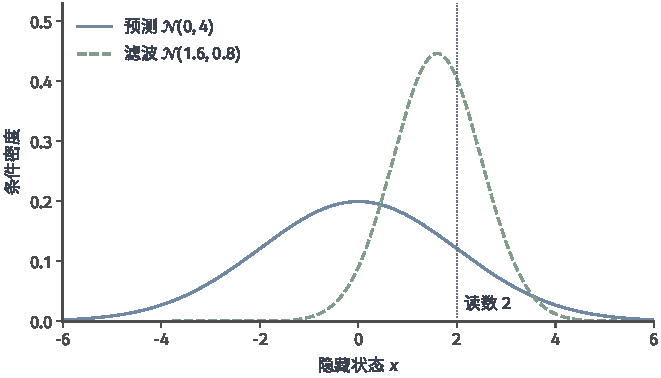
\includegraphics[width=\linewidth]{figures/00-shared/mathematical-preliminaries-lower/02-dynamical-systems-control-decision-and-games/matplotlib/dynamical-kalman-density-update/figure.pdf}
  \caption{独立标量教学例的预测$\mathcal N(0,4)$与后验$\mathcal N(1.6,0.8)$，
 实际读数$y=2$、观测噪声方差$1$。第二个高斯参数是方差；
 本图不是贯穿温度模型的参数设定。}
 \label{fig:dynamical-kalman-density-update}
\end{figure}
\FloatBarrier

若状态更新为$\bm x_{t+1}=\bm f_t(\bm x_t)+\bm w_{t+1}$，
观测为$\bm y_t=\bm h_t(\bm x_t)+\bm v_t$，查询仍是同一个滤波分布，
只是高斯闭合一般失效。扩展Kalman滤波（EKF）在滤波均值附近以
$\bm F_t=D\bm f_t(\bm m_{t\mid t})$传播协方差，
预测均值取$\bm f_t(\bm m_{t\mid t})$；
在预测均值处以$\bm H_{t+1}=D\bm h_{t+1}(\bm m_{t+1\mid t})$
构造创新协方差和增益。它把局部函数替换为一阶线性函数，
所以通常既忽略曲率对均值的影响，也把后验压回单个高斯。

无迹Kalman滤波（UKF）用确定性sigma点近似非线性矩传播。
例如对$d$维均值$\bm m$与协方差$\bm P=\bm L\bm L^\top$，
取$\kappa\geq0$，点为$\bm m$及
$\bm m\pm\sqrt{d+\kappa}\bm L_{\cdot i}$，权重分别为
$\kappa/(d+\kappa)$与$1/[2(d+\kappa)]$。
它们精确匹配原均值与协方差。将点代入$\bm f$，以加权和、加权外积估计
新均值与协方差，再给协方差加上过程噪声$\bm Q$。
本处采用重新生成点的实现：依据加入$\bm Q$后的预测均值和协方差重新构造sigma点，
再把这组点送入$\bm h$，计算预测观测均值、观测协方差及状态观测交叉协方差。
观测协方差还须加上观测噪声$\bm R$，随后按Kalman的创新与增益公式校正。
重新生成点使观测预测也包含本步新增的过程不确定性。
例如标量线性系统$f(x)=h(x)=x$，旧状态方差$p=1$，过程与观测噪声方差
$q=r=1$，上述步骤给出预测方差$2$、创新方差$3$、交叉方差$2$，故增益为$2/3$，
与精确Kalman公式一致；直接复用未包含$q$的原传播点则无法得到这个结果。
这是简单的非负权重构造，实际UKF还可使用带缩放参数的不同权重。
其近似发生在矩积分和高斯投影，不是把非线性模型变成精确线性模型。

两种方法都可能遗漏多峰后验。例如零均值对称先验配上
$y=x^2+v$，一个明显正的读数可能支持正负两个状态区间。
EKF在$x=0$的观测导数为零；对称sigma点也有零状态观测交叉协方差，
单高斯校正不能表达分裂成两峰的证据。
粒子滤波改用加权经验分布$\sum_i\omega_t^{(i)}\delta_{x_t^{(i)}}$：
从已有粒子按转移核抽下一状态，将权重乘当前似然再归一化，
必要时按权重重采样。其近似对象是整个滤波概率测度，
并用有限样本替代核积分；权重集中、高维与重采样损失多样性仍是限制。
高斯混合则保留多个分量，分别传播和校正，再用似然更新分量权重；
分量合并或剪枝会引入另一种近似。

\subsection{基于完整观测的状态平滑}
滤波只能用到当前时刻为止的读数，适合在线实时估计。但事后做复盘时，我们还掌握了后来的读数，而未来的证据往往能反过来照亮过去——例如事后看到温度后来升得很高，可以推断更早时刻的隐藏状态其实也偏高。
固定终点$T$后，未来读数也能帮助判断旧状态。关键不是再向前预测，
而是把新获得的下一状态分布通过反向条件关系传回去。
在线性高斯条件下，给定$\mathcal Y_t$，
\[
 \begin{bmatrix}\bm x_t\\\bm x_{t+1}\end{bmatrix}
 \sim\mathcal N\left(
 \begin{bmatrix}\bm m_{t\mid t}\\\bm m_{t+1\mid t}\end{bmatrix},
 \begin{bmatrix}
  \bm P_{t\mid t}&\bm P_{t\mid t}\bm A_t^\top\\
  \bm A_t\bm P_{t\mid t}&\bm P_{t+1\mid t}
 \end{bmatrix}\right).
\]
若$\bm P_{t+1\mid t}$可逆，条件高斯公式给出
\begin{align}
 \bm J_t&=\bm P_{t\mid t}\bm A_t^\top\bm P_{t+1\mid t}^{-1},
    \label{eq:dynamical-rts-gain}\\
 \mathbb E[\bm x_t\mid\bm x_{t+1},\mathcal Y_t]
   &=\bm m_{t\mid t}+\bm J_t(\bm x_{t+1}-\bm m_{t+1\mid t}),
    \label{eq:dynamical-rts-one-step-conditional-mean}\\
 \operatorname{Cov}(\bm x_t\mid\bm x_{t+1},\mathcal Y_t)
   &=\bm P_{t\mid t}-\bm J_t\bm P_{t+1\mid t}\bm J_t^\top.
    \label{eq:dynamical-rts-one-step-conditional-covariance}
\end{align}
这里的$\bm J_t$关联相邻状态，不是由当前传感器直接得到的Kalman增益。

\begin{theorem}[有限时域RTS平滑]
 \label{thm:dynamical-rts-smoother}
 在有限时域Kalman条件及每个$\bm P_{t+1\mid t}$可逆条件下，
 从终点$(\bm m_{T\mid T},\bm P_{T\mid T})$向后递推
 \begin{align}
  \bm m_{t\mid T}
   &=\bm m_{t\mid t}+\bm J_t(\bm m_{t+1\mid T}-\bm m_{t+1\mid t}),
       \label{eq:dynamical-rts-smoothed-mean}\\
  \bm P_{t\mid T}
   &=\bm P_{t\mid t}
         +\bm J_t(\bm P_{t+1\mid T}-\bm P_{t+1\mid t})\bm J_t^\top,
       \label{eq:dynamical-rts-smoothed-covariance}
 \end{align}
 精确给出$\bm x_t\mid\mathcal Y_T$的高斯均值与协方差。
\end{theorem}
\begin{proof}
 给定$\bm x_{t+1}$后，未来状态和观测与更早状态条件独立，因此
 $P(\mathrm d\bm x_t\mid\bm x_{t+1},\mathcal Y_T)
   =P(\mathrm d\bm x_t\mid\bm x_{t+1},\mathcal Y_t)$。
 全概率公式给出后向因子化
 \begin{equation}
  P(\mathrm d\bm x_t\mid\mathcal Y_T)
   =\int P(\mathrm d\bm x_t\mid\bm x_{t+1},\mathcal Y_t)
                   P(\mathrm d\bm x_{t+1}\mid\mathcal Y_T).
  \label{eq:dynamical-rts-backward-factorization}
 \end{equation}
 将一步条件均值对$\bm x_{t+1}\mid\mathcal Y_T$取期望，
 塔式性质得到平滑均值公式。全协方差公式分成两项：条件内协方差为
 $\bm P_{t\mid t}-\bm J_t\bm P_{t+1\mid t}\bm J_t^\top$，
 条件均值的协方差为$\bm J_t\bm P_{t+1\mid T}\bm J_t^\top$；
 相加即得平滑协方差。一步条件核的均值为仿射函数、协方差不依赖下一状态，
 与高斯下一状态混合仍为高斯。从$T$向后归纳，完成全部时刻的结论。
\end{proof}

前向保存每步滤波与预测的均值、协方差，后向依次计算$\bm J_t$及上述两式，
就是Rauch--Tung--Striebel（RTS）平滑算法\scite{math-rauch1965smoothing}
未来观测影响过去的条件分布，不改变已经发生的物理状态。

\begin{example}[未来观测降低过去状态的不确定性]
 \label{ex:dynamical-scalar-rts-update}
 用独立随机游走例$x_1=x_0+w_1$、$y_1=x_1+v_1$，
 取$m_{0\mid0}=0,P_{0\mid0}=1,Q_1=1,R_1=2/3$，
 初值及两类噪声相互独立，且均为零均值高斯。
 观察$y_1=2$后，$m_{1\mid0}=0,P_{1\mid0}=2$，
 $K_1=3/4,m_{1\mid1}=3/2,P_{1\mid1}=1/2$。
 于是$J_0=1/2$，$m_{0\mid1}=3/4$，
 $P_{0\mid1}=1+\frac14(\frac12-2)=5/8$。
 在时刻$0$尚不能使用这个结果；此时只有均值$0$、方差$1$的初始先验。

 这里每一步的算术都可以顺次核对。先由
 $P_{1\mid0}=P_{0\mid0}+Q_1=1+1=2$得到预测方差，再看增益
 $K_1=P_{1\mid0}/(P_{1\mid0}+R_1)=2/(2+2/3)=3/4$。读数$y_1=2$比预测均值
 $m_{1\mid0}=0$高出\(2\)，于是滤波均值取预测与读数的加权位置
 $m_{1\mid1}=0+\frac34\times2=3/2$——更接近读数，因为观测噪声方差
 \(2/3\)小于预测方差\(2\)。滤波方差降为
 $P_{1\mid1}=2\times(2/3)/(2+2/3)=1/2$。
 后向一步用
 $J_0=P_{0\mid0}/P_{1\mid0}=1/2$：下一状态比预测高出\(3/2\)，
 按这个比例把一半回传到时刻\(0\)，得$m_{0\mid1}=\frac34$；
 平滑方差$P_{0\mid1}=5/8<1=P_{0\mid0}$，说明关于$x_0$的不确定性
 确实被后来的读数缩小了。

 这组数字应按目标状态的时刻分成两组比较。固定目标$x_1$时，
 尚未取得$y_1$的预测均值、方差为$(0,2)$；加入$y_1$后，
 滤波结果为$(3/2,1/2)$。固定目标$x_0$时，无观测的先验为$(0,1)$；
 取得后续读数$y_1$后，平滑结果变为$(3/4,5/8)$。
 每组都保持目标状态不变，只增加所用的观测信息。

 在时刻$0$，$y_1$尚未获得，因此只能使用$x_0$的先验；
 到时刻$1$，既可以用$y_1$估计当前的$x_1$，也可以回溯估计过去的$x_0$，
 两个查询的目标时刻不同。在这个$T=1$的窗口中，$x_1$的平滑已经等于滤波；
 若要比较同一$x_1$在滤波后再吸收更晚读数的变化，还须增加$y_2$等后续观测。
\end{example}

\begin{figure*}[!htb]
  \centering
  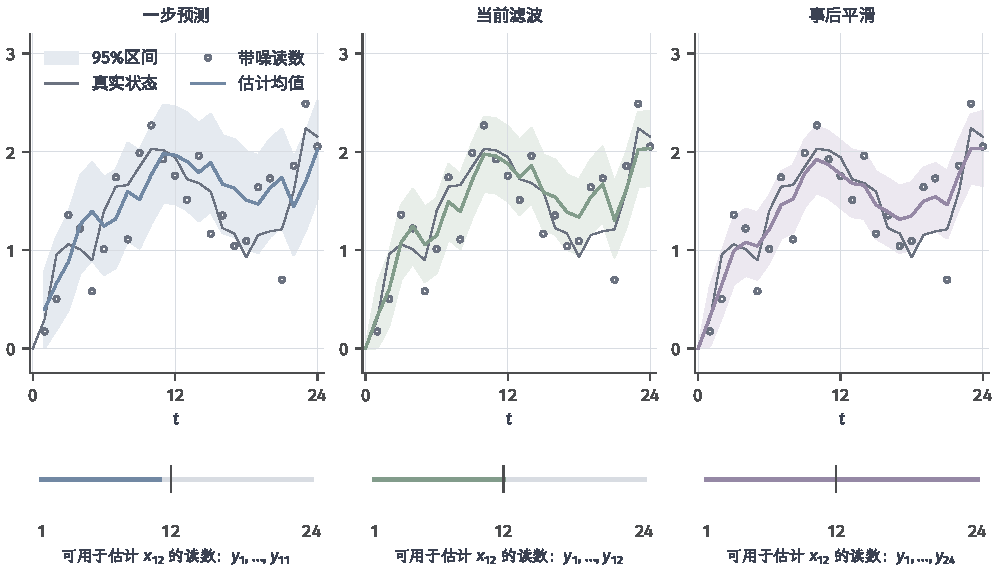
\includegraphics[width=\linewidth]{figures/00-shared/mathematical-preliminaries-lower/02-dynamical-systems-control-decision-and-games/matplotlib/action-state-temperature-inference/figure.pdf}
  \caption{与图~\ref{fig:action-state-temperature-layers}完全相同的温度轨迹及读数。
 三栏分别画一步预测、滤波与固定终点$T=24$的平滑均值和逐时刻$95\%$高斯区间，
 灰线为实际状态，圆点为读数；区间不是整条路径同时覆盖的置信带。
 下方以$t=12$为例标出可用观测范围。已知$x_0=0$，给定$u_t=0.4$，
 过程、观测方差仍为$0.04,0.09$。平滑的信息优势不是额外的在线能力。}
 \label{fig:action-state-temperature-inference}
\end{figure*}

沿用上述有限时域线性高斯条件，有$\bm P_{t\mid T}\preceq\bm P_{t\mid t}$，
即滤波协方差减去平滑协方差是半正定矩阵。这也可从RTS协方差公式向后归纳：
终点两者相等，下一步的平滑协方差不超过其预测协方差，夹乘$\bm J_t$后仍为半正定差。
但某一条实现上的均值误差不必
每个时刻都更小。条件均方误差的保证与某一次噪声实现上的误差是不同对象。
若预测协方差奇异，须在其仿射支持上条件化，广义逆只是计算工具，
还要检查条件状态是否属于支持，不能只替换逆号。
非线性近似平滑可沿相同后向关系用局部线性化或sigma点估计相邻状态的交叉矩；
粒子平滑则近似反向核或路径权重。无论采用哪种表示，使用$\mathcal Y_T$
这一信息条件都不改变。

\subsection{基于完整观测的联合轨迹推断}
各时刻边缘分布回答“那一刻可能在哪里”，整条路径后验还要回答“这些状态如何
一起出现”。在共同观测密度条件下，
\begin{equation}
 P(\mathrm d\bm x_{0:T}\mid\bm y_{1:T})
   =\frac1{Z(\bm y_{1:T})}\,
      \pi_0(\mathrm d\bm x_0)
      \prod_{t=0}^{T-1}K_t(\bm x_t,\mathrm d\bm x_{t+1})
      \prod_{t=1}^Tg_t(\bm y_t\mid\bm x_t),
 \label{eq:action-state-trajectory-posterior}
\end{equation}
其中证据$Z$是分子对路径的积分，要求$0<Z<\infty$。
乘积记号按转移核的迭代积分理解，不预设状态本身有Lebesgue密度。
每个平滑边缘由这一个联合后验积分而来；反过来，只给全部边缘并不能恢复跨时刻关联。

若损失为$\sum_t\|\bm x_t-\bm a_t\|^2$，联合条件均值的各分量就是
$\bm m_{t\mid T}$，因此逐时刻平滑均值同时组成最小化该可加平方损失的路径输出。
在线性高斯模型中，把所有状态堆叠为$\bm X$后，后验仍为联合高斯。
协方差$\bm\Sigma\succ\bm0$时，其密度正比于
$\exp[-(\bm X-\bm m)^\top\bm\Sigma^{-1}(\bm X-\bm m)/2]$，
故联合众数为$\bm m$，也与各时刻的边缘众数一致。
这是一项高斯结构结论，不是所有后验的性质。

若$\bm\Sigma$奇异，后验集中在仿射支持
$\bm m+\operatorname{range}(\bm\Sigma)$，没有全维Lebesgue密度。
记$r=\operatorname{rank}(\bm\Sigma)$。若$r=0$，后验就是点质量$\delta_{\bm m}$，
直接取$\bm m$为输出。若$r>0$，写$\bm\Sigma=\bm U_r\bm\Lambda_r\bm U_r^\top$，
在支持坐标$\bm z=\bm U_r^\top(\bm X-\bm m)$中才有非退化高斯密度；
其唯一众数为$\bm z=\bm0$，对应$\bm m$。
条件高斯使用广义逆时也须要求所给证据位于其支持内；
支持外的条件值属于零概率事件，公式不能赋予一个未经指定的后验意义。

非高斯下可直接看出区别。设两个时刻的联合后验为
\[
 \begin{aligned}
  P(x_0=0,x_1=0)&=0.40,\\
  P(x_0=0,x_1=1)&=0.25,\\
  P(x_0=1,x_1=1)&=0.35.
 \end{aligned}
\]
其他组合概率为零。它可由初始概率$(0.65,0.35)$和转移
$P_{00}=8/13,P_{01}=5/13,P_{11}=1$生成，再配无信息观测。
时刻$0$的边缘众数为$0$，时刻$1$的边缘众数为$1$；
拼接得到$(0,1)$，联合概率只有$0.25$，低于联合最优路径$(0,0)$的$0.40$。
逐点多数意见没有保留跨时刻相容性的全部权重。

有限状态的联合MAP可沿链做最大乘积或Viterbi递推，
而边缘查询沿链求和；其局部函数计算回见图论。
连续非高斯模型可能用路径优化求一个MAP，也可能用粒子或Monte Carlo方法
近似整个后验；前者不是后者的替代品。
例如由$\bm x_T\mid\mathcal Y_T$抽样，再逐步按反向条件核抽
$\bm x_t\mid\bm x_{t+1},\mathcal Y_t$，得到的是有关联的后验路径；
独立从每个平滑边缘抽样会丢掉这些关联。
相关工具可参考\BookPartRef{part:graphs}{卷1《数学准备：计算、分析与几何》的“图”部分}。

本节的精确结论都在有限时域成立。稳态增益、极限协方差及估计误差的长期稳定性，
仍需可检测性、噪声作用方向等系统条件；这些问题交由
\BookChapterRef{chap:control-theory}{第~\ref{chap:control-theory}章}处理。在那里输入才由反馈主动选择，
本章一直把$\bm u_t$当作已给定量。

\section{本章小结}
\label{sec:dynamical-systems-state-estimation-summary}

同一温度模型中的演化规律、真实轨迹与传感器读数承担不同职责。初值和输入给出一次初值问题；过程噪声使轨迹成为随机对象；观测噪声产生用于推断的记录。当前状态只有保存了接续演化所需的信息，才能独自支撑递推。历史窗口的有限投影可以保留指定特征，但闭合更新、表示误差与稳定性仍需分别检查。

给定规律以后，求解轨迹与求解分布也有不同输出。线性传播把各时刻输入的作用累计为和或积分，仿射复合允许并行扫描。Brownian累计通过均方延拓定义，Poisson累计按事件求和；前者的二次变差与后者的有限跳幅决定两类换元修正。未知状态进入系数后才形成随机初值方程。状态分布可以由矩方程或密度方程传播，带噪观测下的状态推断则另用条件规律。

极限分析必须说明让哪个量变化。物理时间增长时研究平衡、极限集合、采样分布和时间平均；固定有限时域而缩小步长时研究轨迹逼近；随机求根中增加算法迭代次数时研究变量更新。精确连续演化稳定不保证任意数值步长稳定，单次有限时域模拟准确也不保证长期采样达到目标分布。强误差使用共同噪声比较状态，弱误差比较测试函数期望，所需条件和收敛阶不同。

扰动分析比较改变初值或输入后的轨迹。有限时间内连续依赖、全部未来保持接近以及误差最终消退，是不同强度的保证；谱条件、Lyapunov下降和输入累计界各自支持相应结论。预测、滤波、平滑和联合轨迹推断再按可用观测范围与查询对象分开，明确输出条件均值、边缘分布还是完整轨迹。

本章把行动序列视为已经给定。\BookChapterRef{chap:control-theory}{第~\ref{chap:control-theory}章}将选择可实施策略并检查可达性、稳定与约束，\BookChapterRef{chap:policy-value-and-optimization}{第~\ref{chap:policy-value-and-optimization}章}则进一步比较策略价值。演化模型和状态推断为这些任务提供条件，单靠轨迹求解仍不能决定怎样行动最合适。

\chapter{随机序列与随机过程}
\label{chap:random-sequences-and-processes}
\label{chap:stochastic-processes-and-approximation}

同一传感器反复读数时，每次噪声可以相互独立，也可以共享一个缓慢变化的背景。即使单次读数具有相同的分布，重复平均的误差和长期行为仍可能不同。前两章建立了随机变量、联合分布、分布变换与差异的工具；现在需要把这些工具用于一整族共同定义的随机读数，说明索引之间怎样联系以及整条实现怎样变化。

本章把有限时刻的联合规律、历史条件与样本路径放在同一概率模型中，再研究累计计算。固定预算下要控制大偏差的概率，预算增长后要判断平均、缩放误差、状态分布与路径各自趋向什么；这两类保证承担不同的任务。采样积分沿用给定的概率规律，展示怎样在保持积分目标的同时调整抽样及样本贡献。概率规律未知时的估计、预测与检验留到下一章讨论。

\section{随机序列与过程的表示}
\label{sec:rv-sequences-processes}
\label{sec:stoch-process-joint-laws}
\label{sec:rv-sequences}

\subsection{共同概率空间上的随机序列与过程}
\label{sec:stoch-common-space-sequences}

反复测量得到的\(X_1,X_2,\ldots\)必须一起定义，才能说明两次读数是否共享噪声。索引\(n\)记录测量轮次；把轮次换成连续时间后，同样的思路给出随机过程。变量族的共同概率空间保留了各次结果之间的联系。
\begin{definition}[随机序列]
\label{def:rv-random-sequence}
同一概率空间上的可测映射族\((X_n)_{n\in\mathbb N}\)称为\term{随机序列}（random sequence）。固定\(n\)得到一个随机变量，固定\(\omega\)得到确定的实现序列
\((X_n(\omega))_{n\in\mathbb N}\)。取值空间可以是实数、向量或其他指定可测空间。
\end{definition}
例如取相互独立的噪声\((\varepsilon_i)\)，并取与全部噪声独立的非退化可积背景变量\(\Theta\)。这些噪声、共享背景的读数
\(X_i=\Theta+\varepsilon_i\)和累计和
\(S_n=\sum_{i=1}^n\varepsilon_i\)都是随机序列，但具有不同的联合关系。噪声序列的各项相互独立；读数序列的各项共享背景\(\Theta\)；累计和序列的相邻项则共享此前的全部增量。即使各项边缘相同，也不能据此选用独立样本平均的结论。这里\(n\)可以是试验编号；当它表示物理时间或算法轮次时，历史信息的解释才进一步进入模型。

\label{sec:rv-paths}
% Baseline S:32-36
随机过程允许索引取自更一般的集合。时间索引可以离散或连续，空间索引也可以标记图上的顶点或欧氏空间的位置；指定索引集合后，各坐标仍须作为同一概率空间上的随机变量共同定义。
\begin{definition}[随机过程]
  \label{def:stoch-process}
  给定概率空间\((\Omega,\mathcal F,\mathbb P)\)、索引集\(T\)和状态可测空间\((\mathcal X,\mathcal A)\)，\term{随机过程}（stochastic process）是一族随机变量\((X_t)_{t\in T}\)，其中每个\(X_t:\Omega\to\mathcal X\)均可测。
\end{definition}

\subsection{基于有限维分布的过程表示}
\label{sec:rv-finite-dimensional-laws}
设每次只能观察有限个时刻，我们可以分别指定这些读数的联合分布。问题在于：删去部分时刻或重排时刻后，这些指定还能不能来自同一个过程，也就是彼此是否相容。建立共同过程之后，路径能否连续仍需另外的增量条件；一列近似过程的路径极限则由第~\ref{sec:rv-path-convergence}节研究。

只给每个时刻的边缘分布，无法判断相邻时刻是同向、独立还是反向变化。有限维分布是在任意有限时刻集合上给出
\(\mathcal L(X_{t_1},\ldots,X_{t_m})\)，把这种共同变化也保存下来。

要把这些有限观测放到同一个空间中，记\(E^T\)为全部映射\(x:T\to E\)的集合。
其乘积\(\sigma\)代数由有限坐标柱集生成；这类集合的形式是
\[
 \{x\in E^T:(x(t_1),\ldots,x(t_m))\in B\},
\]
其中\(B\)为有限积\(E^m\)中的可测集。它只检查有限个坐标是否满足某项条件，再由可数集合运算生成更多事件；每个坐标评价\(x\mapsto x(t)\)因此可测。

这里的标准Borel条件指可测空间可与某个完备可分度量空间中某个Borel子集的可测结构建立可测同构；实数、有限维欧氏空间及有限或可数离散空间都满足这一条件。它排除仅靠有限维相容性仍无法在任意可测结构上完成扩张的情形。

\begin{theorem}[Kolmogorov扩张的标准Borel版本]
\label{thm:rv-kolmogorov-extension}

设状态空间\(E\)是标准Borel空间，\(T\)为任意索引集。若给定每个有限索引集合\(J\subset T\)上的概率测度\(P_J\)，且对有限集合\(J\subset K\)，从\(E^K\)投影到\(E^J\)把\(P_K\)推送为\(P_J\)，则存在唯一的概率测度定义在\(E^T\)的乘积\(\sigma\)代数上，使各坐标过程具有这些有限维分布。
用有序时刻元组表示时，还必须满足重排坐标的相容性。
\end{theorem}
相容性意味着同一个两时刻问题，不论直接指定还是从三时刻问题删掉一个坐标，都应得到同一答案。高斯过程的半正定核会提供一组相容的高斯向量，因而可用此定理建立过程。扩张定理不同时承诺它落在连续路径空间中，也不保证
\((t,\omega)\mapsto X_t(\omega)\)联合可测。这里的唯一性只针对乘积\(\sigma\)代数中的事件；整条路径的连续性还须另行建立版本及适合的路径空间。

\subsection{基于样本路径的过程表示}
\label{sec:stoch-sample-path-representation}
离散时间通常取\(T=\mathbb N_0\)，连续时间取\(T=[0,\infty)\)。固定时刻\(t\)，
\(\omega\mapsto X_t(\omega)\)是随机变量；固定基础结果\(\omega\)，
\(t\mapsto X_t(\omega)\)是样本路径。所谓连续时间只规定索引可以任取实数，不规定取值连续，更不规定路径连续。

图~\ref{fig:rv-paths}中，沿横轴看一条线，是一次实现随时间怎样变化；沿竖线看多个交点，是同一时刻在不同实现中的结果。右连续阶梯路径可以在连续时间定义却只取整数；连续实值路径也可能非常粗糙。稍后的Poisson和Brownian过程分别给出这两种情形的正式模型。
\begin{figure}[htbp]
  \centering
  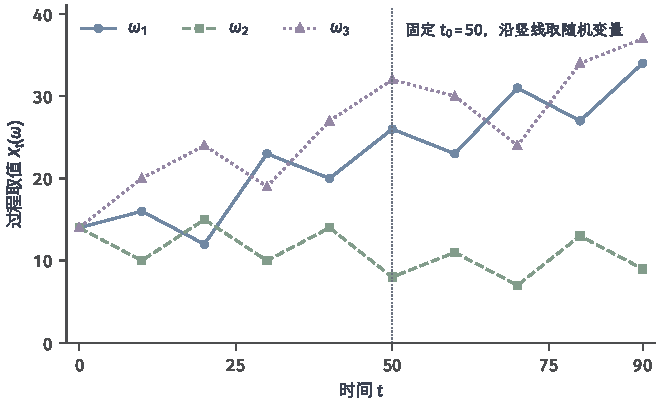
\includegraphics[width=\linewidth]{figures/00-shared/mathematical-preliminaries-lower/01-random-variables-distributions-and-causality/matplotlib/rv-paths/figure.pdf}
  \caption{同一过程的路径与时刻截面是不同对象。图为人为给定的三条示意路径，竖虚线固定时刻\(t_0\)；交点展示该时刻可能出现的不同值，并非用三条路径估计出的概率密度。}
\label{fig:rv-paths}
\end{figure}

若对每个固定\(t\)，\(\mathbb P(X_t=Y_t)=1\)，称\(X,Y\)互为版本；若
\(\mathbb P(\forall t,\ X_t=Y_t)=1\)，则称不可区分。不可数时间集上，两者不同。
例如\(U\)在\([0,1]\)均匀分布，\(X_t=\mathbb I_{\{t=U\}}\)、\(Y_t=0\)：
每个固定时刻两者几乎必然相等，但每条\(X\)路径都在某个时刻出现尖点。
若两个版本都具有右连续路径，则先在可数稠密时刻同时相等，再用右连续性推广，才得到不可区分。

描述连续路径的粗糙程度时，称\(x\)在紧时间区间上具有正指数\(\alpha\)的Hölder连续性，是指存在有限\(C_x\)，使
\[
 |x(t)-x(s)|\leq C_x|t-s|^\alpha
 \quad\text{对区间内所有 }s,t\text{成立}.
\]
随机路径允许常数\(C_x\)依赖具体实现。\(\alpha=1\)就是Lipschitz条件；在短时间差上，较小的正指数给出较弱的约束。例如\(\sqrt t\)满足
\(|\sqrt t-\sqrt s|\leq|t-s|^{1/2}\)，却在零点附近不满足Lipschitz条件。这里是路径正则性，与同名的Hölder积分不等式不同。

得到连续版本的一项常用充分条件是Kolmogorov连续性准则：若在紧时间区间上存在
\(p>0,\beta>0,C<\infty\)，使
\[
\mathbb E|X_t-X_s|^p\leq C|t-s|^{1+\beta},
\]
则存在连续版本，并可取得任意小于\(\beta/p\)的正Hölder指数；该条件本身不保证达到端点\(\beta/p\)。条件控制的是整族短时增量，不能由每个时刻分布连续推出。对Brownian增量，四阶矩为\(3|t-s|^2\)，足以给出连续版本；更高阶矩可把Hölder指数推进到任意小于\(1/2\)。

\subsection{随机误差的收敛与量级}
\label{sec:stoch-convergence-criteria}
重复测量时，一个自然的问题是：样本均值的误差是否会随样本数增多而缩小。要严格表述“缩小”，先要说明控制的是哪个量：大偏差发生的概率、整条样本路径，还是平均平方误差。下面先约定这几种收敛判据，后文在具体估计问题中使用它们，并在第~\ref{sec:rv-sequence-process-convergence}节证明彼此的关系。
\paragraph{随机结果的收敛判据}
\begin{definition}[随机变量的收敛]
  \label{def:probability-random-convergence}
以下依概率、几乎必然和\(L^p\)收敛要求\(X_n,X\)定义在同一概率空间上；依分布收敛只要求它们的分布有定义。若对每个\(\varepsilon>0\)，
\[ \mathbb{P}(|X_n-X|>\varepsilon)\to0, \]
就称\(X_n\)依概率收敛到\(X\)，记作\(X_n\to_{\mathbb{P}}X\)。它允许小概率坏事件随\(n\)改变，只要求每个固定容差外的概率趋于零。

若
\[ \mathbb{P}\left(
    \lim_{n\to\infty}X_n=X\right)=1, \]
就称\(X_n\)几乎必然收敛到\(X\)，记作\(X_n\to_{\mathrm{a.s.}}X\)。它要求除一个
固定零测集外，每条样本路径最终都收敛，因而比依概率收敛更强。

对\(1\leq p<\infty\)，若\(X_n,X\in L^p(\mathbb P)\)且\(\mathbb{E}[|X_n-X|^p]\to0\)，就称\(X_n\)在\(L^p\)中收敛。特别地，\(p=2\)称为均方收敛。

若对\(X\)的每个分布函数连续点\(x\)，都有
\[ F_{X_n}(x)\to F_X(x), \]
就称\(X_n\)依分布收敛到\(X\)，记作\(X_n\Rightarrow X\)。它只比较边缘分布，不要求变量定义在同一概率空间上。

\end{definition}

\paragraph{随机误差的概率阶}
渐近分析还要比较随机误差与某个确定尺度的相对大小，例如判断余项相对于主项是否可以忽略。下面的概率阶记号把这种比较写成可以直接检验的概率条件。
\begin{definition}[概率阶记号]
  \label{def:statistics-probability-order}
\term{概率有界}（bounded in probability）把“随机量不会随\(n\)逃向无穷”写成
可检验的概率条件。若对每个\(\epsilon>0\)，都存在有限常数\(M\)和整数\(n_0\)，使
\[
  \sup_{n\geq n_0}\mathbb{P}(|X_n|>M)<\epsilon,
\]
就记\(X_n=O_{\mathbb{P}}(1)\)。若\(X_n\to_{\mathbb{P}}0\)，则记
\(X_n=o_{\mathbb{P}}(1)\)。对确定正数列\(a_n\)，约定\(X_n=O_{\mathbb P}(a_n)\)与\(X_n=o_{\mathbb P}(a_n)\)分别表示\(X_n/a_n=O_{\mathbb P}(1)\)与\(X_n/a_n=o_{\mathbb P}(1)\)。
\end{definition}

\section{随机序列与过程的依赖关系}
\label{sec:stoch-process-dependence}
一组读数可以共享同一背景，也可以随状态逐步演化。要判断重排记录、压缩历史或平移时间会保留哪些概率结论，需要分别规定联合规律的对称性、下一状态的条件规律、下一读数的条件均值与时间平移的规律。这些条件可以同时成立，不能互相替代。

\subsection{序列重排下的交换关系}

若一批观测没有需要保留的顺序，可以检查重排记录以后联合规律是否改变。这一对称要求只比较重排前后的规律，不要求各项独立；共享同一背景的观测也可能满足它。
\label{sec:rv-exchangeability}
% Baseline P:2279-2289
\begin{definition}[可交换随机变量]
  \label{def:probability-exchangeability}
随机变量\(Z_1,\ldots,Z_m\)若对每个排列\(\pi\)都有
\[ (Z_1,\ldots,Z_m)
  \overset{\mathrm{d}}{=}(Z_{\pi(1)},\ldots,Z_{\pi(m)}), \]
就称它们\term{可交换}（exchangeable）。
\end{definition}
独立同分布蕴含可交换，但反向不成立。
例如先抽取取值于\([0,1]\)的非退化随机概率\(\Theta\)，再条件于\(\Theta\)独立生成Bernoulli观测；边缘上这些观测可交换，却因共享\(\Theta\)而相关。

可交换性不提供样本平均的独立乘积结构，因而不能直接代入Hoeffding证明。
它提供的是标签位置的对称性：若评分规则在重排观测时只把分数作同样的重排，
并且分数几乎必然没有并列，则每个分数占据每个秩的概率都是\(1/m\)。
因为所有标签机会相同，而每个秩又恰由一个标签占据，概率总和必须为\(1\)。
有并列时，可为每个分数附加一个服从\(\operatorname{Unif}(0,1)\)的随机数，
这些随机数相互独立，并且独立于全部分数。
把分数按大小排序，分数相同时再按附加的随机数排序；这样既保留对称性，又消除并列，从而恢复均匀的秩。
若采用不随机化的并列规则，则通常只能得到相应的保守概率界。
后面的共形预测会明确区分这两种处理，使用它们各自的有限样本结论。
例如共享参数\(\Theta\sim\operatorname{Beta}(2,2)\)，给定\(\Theta\)后
\(X_i\)独立服从\(\operatorname{Bernoulli}(\Theta)\)。每个边缘的成功率为\(1/2\)，但对\(i\ne j\)，塔式性质给出
\[
\operatorname{Cov}(X_i,X_j)
=\mathbb E[\Theta^2]-(\mathbb E\Theta)^2
=\operatorname{Var}(\Theta)=\frac1{20}.
\]
因此\(\mathbb P(X_1=X_2=1)=0.3\)，大于独立情况下的\(0.25\)。
共享背景使一串成功更常一起出现，却没有偏爱某个观测编号。有限可交换性本身不保证一定存在这样的独立混合表示；本例是可交换依赖的一种构造。

\subsection{历史条件下的状态依赖}

预测下一时刻时，完整历史通常含有很多记录。若当前状态已经概括其中与下一步有关的信息，给定当前状态后继续加入旧记录就不应改变下一步条件分布。Markov关系将这个建模要求写成条件分布的等式。
\label{sec:rv-markov}
\label{sec:stoch-martingales-stopping-sequential-concentration}
先约定时刻\(t\)已知哪些记录。滤过使“完整历史”成为可用于条件期望的数学对象；适应性检查当前状态是否已经可知，可预测性则检查下一步所用系数是否在新噪声揭晓前确定。
% Baseline S:371-384
\begin{definition}[滤过、适应与可预测性]
  \label{def:stoch-filtration-adaptation-predictability}
在概率空间
$(\Omega,\mathcal{F},\mathbb{P})$上，令每个$\mathcal{F}_t$都是
$\mathcal{F}$的子$\sigma$代数，并且
\[
  \mathcal{F}_0\subseteq\mathcal{F}_1\subseteq\cdots\subseteq\mathcal{F}.
\]
这列递增的子$\sigma$代数称为\term{滤过}（filtration），可以理解为随时间增长的信息。
随机变量$X_t$若对
$\mathcal{F}_t$可测，就称它在时刻$t$已经可知；若每个$t$都如此，称$(X_t)$适应于该滤过。对$t\geq1$，过程$(H_t)$若$H_t$对
$\mathcal{F}_{t-1}$可测，就称为\term{可预测过程}（predictable process）。
\end{definition}
这里的“可预测”不是说$H_t$没有随机性，而是说它可以由第$t$次新噪声到来之前的信息确定。
% Baseline S:441-447
逐步观测还可能在读数首次越过阈值时结束，结束轮次因此是随机的。可实施的停止规则必须只用已经取得的记录：到当前轮次就能判断是否已经结束。下面的条件排除依赖未来记录的停止选择。
\begin{definition}[停时]
  \label{def:stoch-stopping-time}
  相对于滤过\((\mathcal F_t)_{t\geq0}\)，取值于\(\mathbb N_0\cup\{\infty\}\)的随机时刻$\tau$若满足$\{\tau\leq t\}\in\mathcal{F}_t$对每个整数$t\geq0$成立，就称为\term{停时}（stopping time）。
\end{definition}
到时刻$t$为止已有的信息足以判断是否已经停止；“最后一次
达到最大值的时刻”通常需要看到未来，不一定是停时。

% Baseline S:69-131
\begin{definition}[Markov链]
  \label{def:stoch-markov-chain}
设$(Z_t)_{t\geq0}$取值于可测空间$(\mathcal{Z},\mathcal{A})$。若对每个
$B\in\mathcal{A}$，
\[
  \mathbb{P}(Z_{t+1}\in B\mid Z_0,\ldots,Z_t)
  =
  \mathbb{P}(Z_{t+1}\in B\mid Z_t),
\]
则称$(Z_t)$为\term{Markov链}（Markov chain）；上述条件等式按几乎必然意义理解。
\end{definition}
这个条件不是说过去没有影响，而是
说当前状态已经保存了预测下一步所需的全部历史信息。
即使当前状态足以预测下一步，同一个状态在上午和晚上也可能使用不同的转移规律。若进一步假设规律不随轮次改变，就可以反复使用同一个核，并用核的复合计算多步分布。
\begin{definition}[时间齐次Markov链]
  \label{def:stoch-time-homogeneous-chain}
  若存在从\((\mathcal Z,\mathcal A)\)到自身的概率核\(P\)，使所有\(t\geq0\)、\(B\in\mathcal A\)都满足
  \[ \mathbb P(Z_{t+1}\in B\mid Z_t)=P(Z_t,B)\quad\text{几乎必然}, \]
  则该Markov链称为\term{时间齐次的}（time-homogeneous）。
\end{definition}
时间齐次描述机制不变，不代表$Z_t$的边缘分布不随时间改变\scite{math-meyn2009markov}。

概率核的两项要求见\BookDefinitionRef{def:probability-kernel}{定义~\ref{def:probability-kernel}}：每个状态对应合法的下一步分布，而每个事件的概率随当前状态可测地变化。对有界可测函数$f$，记
\[
  Pf(z)=\int_{\mathcal{Z}}f(z')P(z,\mathrm{d}z').
\]
两个核的复合按
\[
  (PQ)(z,B)
  =
  \int_{\mathcal{Z}}Q(z',B)P(z,\mathrm{d}z')
\]
定义；它表示先按$P$走一步，再按$Q$走一步。令$P^0(z,B)=\mathbb{I}\{z\in B\}$，
$P^{m+1}=P^mP$，则时间齐次链满足
\begin{equation}
  \mathbb{P}(Z_{t+m}\in B\mid Z_t=z)=P^m(z,B),
  \qquad
  P^{m+n}(z,B)
  =
  \int_{\mathcal{Z}}P^n(z',B)P^m(z,\mathrm{d}z').
  \label{eq:stoch-chapman-kolmogorov}
\end{equation}
第一个等式作为条件分布恒等式只要求对\(Z_t\)的分布几乎处处成立；不可达状态上的条件版本并不由观测规律确定。核的复合则在每个\(z\)上有定义。第二个等式称为\term{Chapman--Kolmogorov关系}。证明可直接使用条件概率的塔式性质：
给定$Z_{t+m}=z'$后，Markov性质把后$n$步的条件概率化为$P^n(z',B)$；再对
$Z_{t+m}$在给定$Z_t=z$时的分布$P^m(z,\mathrm{d}z')$积分，就得到右侧。取$n=1$
并归纳，还同时证明了第一个等式及核幂确实给出多步转移。

核给出了分布怎样前进一步。现在反过来寻找一种初始分布，使前进一步后各事件的概率都保持不变：对旧状态分布混合下一步核，得到的仍是原分布。这样的分布是分布更新的不动点，而不是要求单个状态停止移动。
\begin{definition}[平稳分布]
  \label{def:stoch-stationary-distribution}
概率分布$\pi$若满足
\begin{equation}
  \pi(B)=\int_{\mathcal{Z}}P(z,B)\,\pi(\mathrm{d}z),
  \qquad B\in\mathcal{A},
  \label{eq:stoch-stationary-distribution}
\end{equation}
就称为$P$的\term{平稳分布}（stationary distribution）。
\end{definition}
若$Z_0\sim\pi$，式
\eqref{eq:stoch-stationary-distribution}保证每个$Z_t$仍服从$\pi$；若从指定状态
$z_0$启动，平稳性本身却没有说明$\mathcal{L}(Z_t)$会趋向$\pi$。恒等转移核
$P(z,B)=\mathbb{I}\{z\in B\}$保持任意分布，但它永远不忘记初态，这已经表明“保持
目标”和“到达目标”是两项不同要求。

% Baseline S:151-163
要验证一张候选分布被转移核保持，可以直接核对上面的积分等式，也可以寻找更容易逐对核验的充分条件。在有限状态下，若每对状态之间的正向流量\(\pi_iP_{i,j}\)都等于反向流量\(\pi_jP_{j,i}\)，对所有来源求和就能保证各处总质量不变。下面把这一逐对流量条件推广到一般状态空间。
\begin{definition}[细致平衡]
  \label{def:stoch-detailed-balance}
概率核\(P\)与概率测度\(\pi\)满足\term{细致平衡}（detailed balance），若以下两个联合测度在\(\mathcal Z\times\mathcal Z\)上相同：
\begin{equation}
  \pi(\mathrm{d}z)P(z,\mathrm{d}z')
  =\pi(\mathrm{d}z')P(z',\mathrm{d}z).
  \label{eq:stoch-detailed-balance}
\end{equation}
\end{definition}
它要求平稳运行时任意两处之间的概率流量正反相等。对$z$积分便得到
\eqref{eq:stoch-stationary-distribution}，所以细致平衡足以推出平稳性。反向不成立：
围绕三个状态单向循环的链可以保持均匀分布，却没有逐边对称的反向流。细致平衡是构造
采样链的便利证书，不是遍历平均成立的必要定义。

\subsection{历史条件下的均值关系}

完整条件分布不变是一项强要求。有时只知道新增量在已有历史下没有平均漂移，方差和其他形状仍可随历史改变。把这类增量累计起来，得到条件均值保持当前值的过程，称为鞅；下面用可积性使这个均值等式有意义。
\label{sec:rv-martingales}
% Baseline S:386-425
\begin{definition}[鞅与鞅差]
  \label{def:stoch-martingale}
可积过程$(M_t)$若适应于$(\mathcal{F}_t)$，并对每个整数$t\geq1$满足
\begin{equation}
  \mathbb{E}[M_t\mid\mathcal{F}_{t-1}]=M_{t-1},
  \label{eq:stoch-martingale-definition}
\end{equation}
就称为\term{鞅}（martingale）。增量$X_t=M_t-M_{t-1}$满足
\begin{equation}
  \mathbb{E}[X_t\mid\mathcal{F}_{t-1}]=0,
  \label{eq:stoch-martingale-difference}
\end{equation}
称为\term{鞅差}（martingale difference）。若条件等式改为\(\mathbb E[M_t\mid\mathcal F_{t-1}]\leq M_{t-1}\)，称\((M_t)\)为超鞅；改为\(\geq\)时称为次鞅。两者也要求每个时刻可积且适应。
\end{definition}
这里的\(t\)是离散整数时刻。连续时间的定义把相邻时刻条件换成：
对任意\(0\leq s\leq t\)，
\(\mathbb E[M_t\mid\mathcal F_s]=M_s\)几乎必然；每个时刻仍须可积且适应。
超鞅与次鞅分别改用\(\leq\)和\(\geq\)。后面的补偿计数与布朗运动均使用这一连续时间版本。
无条件零均值不够：若$X_t$可以由过去
预测，累计和仍可能形成系统漂移；式~\eqref{eq:stoch-martingale-difference}排除的正是
这种可利用的条件平均。

\begin{example}[公平随机游走与按过去下注]
  \label{ex:stoch-predictable-betting}
  设$\varepsilon_t$独立取$\{-1,1\}$，两种取值概率均为$1/2$，并令
  $\mathcal{F}_t=\sigma(\varepsilon_1,\ldots,\varepsilon_t)$。公平随机游走
  $S_t=\sum_{s=1}^{t}\varepsilon_s$是鞅。

  现在允许下注额$H_t$根据过去结果选择，只要求$H_t$对
  $\mathcal{F}_{t-1}$可测，并使$H_t\varepsilon_t$可积。另设\(M_0\)可积且对\(\mathcal F_0\)可测。财富过程
  \[
    M_t=M_0+\sum_{s=1}^{t}H_s\varepsilon_s
  \]
  仍是鞅，因为
  \[
    \mathbb{E}[H_t\varepsilon_t\mid\mathcal{F}_{t-1}]
    =
    H_t\mathbb{E}[\varepsilon_t\mid\mathcal{F}_{t-1}]
    =0.
  \]
  策略可以追涨、反向或在某些历史后停止下注，但只要它不能偷看$\varepsilon_t$，就不能
  改变下一笔收益的条件均值。若$H_t$依赖当前尚未揭晓的$\varepsilon_t$，上面的等式便
  失去依据。
\end{example}
条件均值保持本身没有规定长期极限。定理~\ref{thm:rv-l2-martingale-convergence}将在序列收敛中补充二阶矩有界条件，说明累计误差何时具有路径极限与均方极限。

这里值得先分清两个常被混淆的说法。例~\ref{ex:stoch-predictable-betting}说明“每期条件均值为零”不等于“不能亏损”：公平下注策略的财富可以使已实现路径长期为负，只是这种路径不能用已知历史提前识别。可预测性要求下注额在新噪声揭晓前已经由历史确定；收益增量的零条件均值还需要噪声在该历史下均值为零。两项条件共同支持上面的鞅结论，都不保证单条实现不亏损。相应地，鞅差的零条件均值也不推出增量之间的无条件独立性：增量可以有相同的方差、可以有依赖的绝对值，甚至方差本身随历史变化（例如每期下注额随财富调整），但只要给定历史后条件均值为零，累计和仍是鞅。把鞅差一律当作独立同分布变量，会漏掉允许历史依赖和条件异方差的情形。

第二个区分关乎定义中条件\(\sigma\)代数的选择。条件期望\(\mathbb E[M_t\mid\mathcal F_{t-1}]\)随\(\mathcal F_{t-1}\)变化：信息更多时，条件均值可能不再等于\(M_{t-1}\)。因此同一序列在较粗的信息流下可能是鞅，在较细的信息流下则不是。例如令独立符号\(\varepsilon_t\)等概率取\(\pm1\)，\(M_t=\sum_{s=1}^t\varepsilon_s\)，自然历史为\(\mathcal F_t=\sigma(\varepsilon_1,\ldots,\varepsilon_t)\)。给定\(\mathcal F_{t-1}\)后，下一增量仍均值为零，所以\(M_t\)是鞅。若扩大信息流为\(\mathcal G_t=\sigma(\varepsilon_1,\ldots,\varepsilon_{t+1})\)，则\(M_t\)仍适应，但\(\mathcal G_{t-1}\)已经揭晓\(\varepsilon_t\)，于是\(\mathbb E[M_t\mid\mathcal G_{t-1}]=M_t\)，通常不等于\(M_{t-1}\)。因此独立零均值增量只保证相对于不预先揭晓这些增量的适当历史是鞅，不能保证相对于任意扩大的信息流仍是鞅。使用鞅结论时必须说明信息流是什么，这与条件期望的定义要求一致。

\subsection{时间平移下的分布关系}
\label{sec:rv-stationarity}
% Baseline S:132-149
把观测窗口从今天移到明天后，若整组读数的联合规律保持不变，就可以用时间平移来表达这种稳定的统计结构。这里比较的是窗口中的联合分布；仅保持单时刻的边缘分布，还不足以确定两次读数之间的联系。
\begin{definition}[平稳过程]
  \label{def:stoch-stationary-process}
  离散时间过程\((Z_t)_{t\geq0}\)称为\term{平稳过程}（stationary process），若任意正整数\(m\)、时刻\(t_1,\ldots,t_m\geq0\)及整数\(h\geq0\)都满足
  \[ (Z_{t_1},\ldots,Z_{t_m})\overset{\mathrm d}{=}(Z_{t_1+h},\ldots,Z_{t_m+h}). \]
\end{definition}
对时间齐次Markov链，若$Z_0\sim\pi$且
$\pi P=\pi$，则
\[
  \mathbb{P}(Z_0\in\mathrm{d}z_0,\ldots,Z_m\in\mathrm{d}z_m)
  =
  \pi(\mathrm{d}z_0)
  \prod_{j=1}^{m}P(z_{j-1},\mathrm{d}z_j).
\]
把起点向后平移一格时，先对$z_0$积分，$\pi P=\pi$把$Z_1$的边缘重新化为$\pi$，
其余转移核不变；反复应用便证明所有有限维分布都不随平移改变。因此，从平稳分布启动的
时间齐次链是平稳过程。只知道某一个时刻的边缘分布等于$\pi$，却没有核不变或联合分布
条件时，不能据此断言整个过程平稳。
完整联合分布的平移不变性较强。若当前只计算平均值和二阶误差，可以先保留较少的要求：各时刻均值不变，两次读数的协方差只由相隔多久决定。这个较弱条件足以组织二阶计算，却未必保留全部分布形状。
\begin{definition}[二阶平稳]
\label{def:rv-second-order-stationary}
实值过程二阶矩有限，若均值与时间无关，且
\(\operatorname{Cov}(X_s,X_t)\)只依赖时间差\(t-s\)，称为\term{二阶平稳}（second-order stationarity），也称弱平稳。
\end{definition}
严格平稳加有限二阶矩推出二阶平稳；反向一般不成立。例如相互独立的序列在偶数时刻取标准高斯分布，在奇数时刻等概率取\(\pm1\)。均值均为零，方差均为一，非同时刻协方差均为零，所以二阶平稳，但一维边缘随奇偶变化，并不严格平稳。联合高斯过程则由均值与协方差完全决定有限维规律，因此此时二阶平稳足以推出严格平稳。
Brownian运动和零均值随机游走可以是Markov鞅，但方差随时间增长，不是平稳过程；其增量却可平稳。核的不变分布、从任意初态趋向它，以及过程已经从该分布启动，仍是三项不同命题。

\section{随机序列与过程的生成}
\label{sec:stoch-sequence-process-generation}
依赖条件约束一族已有变量的联合规律；构造模型还要给出能够产生这些联合规律的规则。累计独立增量、反复应用转移核、记录事件到达以及指定高斯协方差，分别形成不同的生成方式。有限分割上的相容概率向量还可让整张概率测度成为随机对象。

\subsection{基于状态转移的随机序列生成}
\label{sec:rv-state-generation}

给定当前状态后抽取一步增量，再重复这一操作，可以生成整条随机序列。随机游走用增量相加确定下一位置；一般Markov链则直接用转移核给出下一状态的条件分布。它们都保留逐步生成的次序，相邻位置之间通常相关。

\subsubsection{基于增量累计的随机游走生成}
\label{sec:rv-random-walk}
给定独立同分布增量\(\xi_i\)，定义
\(S_0=0\)、\(S_n=\sum_{i=1}^n\xi_i\)，称为\term{随机游走}（random walk）。若
\(\mathbb E\xi_i=\mu\)、\(\operatorname{Var}(\xi_i)=\sigma^2<\infty\)，则
\[
\mathbb ES_n=n\mu,\qquad
\operatorname{Var}(S_n)=n\sigma^2,\qquad
\operatorname{Cov}(S_m,S_n)=\min(m,n)\sigma^2.
\]
当\(\sigma^2>0\)且\(m,n\geq1\)时，位置之间的协方差为正，所以不能把不同位置当作独立观测。
\(S_n-n\mu\)相对于增量的自然滤过是鞅，\(S_n\)本身还具有Markov性。
若\(\mathbb P(\xi_i=1)=p\)、\(\mathbb P(\xi_i=-1)=1-p\)，则漂移为
\(2p-1\)、单步方差为\(4p(1-p)\)。取\(p=0.6\)，十步均值为\(2\)、方差为\(9.6\)；某一条十步路径却不必靠近均值。
大数定律控制\(S_n/n\)，当\(\sigma>0\)时，中心极限定理控制
\((S_n-n\mu)/(\sigma\sqrt n)\)；整个折线在缩放下的极限则使用第~\ref{sec:rv-path-convergence}节的路径定理。

\subsubsection{基于转移核的Markov链生成}
Markov核给出一步条件规律：从当前状态出发，下一步可能到哪些状态、各以什么概率。但只凭这一步还不够，还要回答三个问题：多步以后状态如何分布，边缘分布能否趋向某个极限，长期平均又由什么决定。下面分别需要核复合及返回条件。

\paragraph{状态转移与多步分布}
% Baseline S:165-185
\begin{example}[相关的两状态观测]
  \label{ex:stoch-two-state-chain}
  令$Z_t\in\{0,2\}$，并把观测直接取为$Y_t=Z_t$。转移矩阵按状态$0,2$排序为
  \[
    \bm{P}
    =
    \begin{pmatrix}
      0.9 & 0.1\\
      0.2 & 0.8
    \end{pmatrix}.
  \]
  平稳分布为$\bm{\pi}=(2/3,1/3)^\top$，因为
  $\bm{P}^{\top}\bm{\pi}=\bm{\pi}$。在这项平稳分布下，单次观测的均值是
  \[
    \mu=\mathbb{E}_{\pi}[Y]=\frac23.
  \]
  两条跨状态概率流都等于
  $(2/3)\times0.1=(1/3)\times0.2=1/15$，故该链还满足细致平衡。
  从状态$0$启动时，$Y_0$不服从$\pi$；转移规则时间齐次，过程却要经过一段时间才
  接近平稳。
\end{example}
% Baseline S:189-197
这个例子能在两个状态之间来回移动，且允许原地停留。要判断一般链能否忘记初态，需要把这两项作用分开：是否任意状态都能经若干步到达另一个状态，以及返回是否只能发生在某些固定倍数的步数上。不可约性检查前者，周期检查后者。
\begin{definition}[有限链的不可约性与周期]
  \label{def:stoch-finite-irreducibility-period}
  有限状态Markov链满足\term{不可约性}（irreducibility），若对任意状态\(i,j\)存在整数\(m\geq0\)，使\(P^m(i,\{j\})>0\)。若返回步数集合非空，状态\(i\)的\term{周期}（period）定义为
  \[ d_i=\gcd\{m\geq1:P^m(i,\{i\})>0\}. \]
  不可约链的全部状态具有共同周期；该周期为\(1\)时，称链为\term{非周期的}（aperiodic）。
\end{definition}
把相互可达的状态归在一起，得到互达等价类；若从一个类内出发，一步转移不会离开该类，就称它封闭。
不可约性要求所有状态属于同一个互达类，并在有限状态下保证平稳分布唯一。

在前面的两状态例子中，令\(q_t=\mathbb P(Y_t=2)\)。一步转移给出
\[
q_{t+1}=0.1(1-q_t)+0.8q_t=0.1+0.7q_t,
\qquad q_t=\frac13+0.7^t\left(q_0-\frac13\right).
\]
从\(q_0=0\)出发，前两步为\(q_1=0.1,q_2=0.17\)，而不是立即得到
\(1/3\)。不变分布给出递推的不动点；这里的收敛则由偏差系数\(0.7\)另行证明。

\subsection{基于到达计数的随机过程生成}
\label{sec:rv-poisson}
事件到达使状态按次跳变。固定窗口内的计数可以服从Poisson分布，但只有规定不同窗口间的联合关系，才能得到Poisson过程。

\paragraph{事件计数与短时跳跃}
\begin{definition}[齐次Poisson过程]
\label{def:rv-poisson-process}
给定速率\(\lambda>0\)和滤过\((\mathcal F_t)_{t\geq0}\)，计数过程
\((N_t)_{t\geq0}\)称为相对于该滤过的齐次\term{泊松过程}（Poisson process），若它适应于滤过，
\(N_0=0\)几乎必然，路径几乎必然右连续、非减、取非负整数且每次跳跃为一，并满足
\[
N_t-N_s\ \perp\ \mathcal F_s,\qquad
N_t-N_s\sim\operatorname{Poisson}(\lambda(t-s)),
\quad 0\leq s<t.
\]
\end{definition}
这里的平稳性属于增量，而非\(N_t\)本身：计数均值随时间线性增长。
对互不相交、按时间排列的区间，逐步使用独立于过去的条件，便得到增量相互独立。
相对于自然滤过给出过程后，不能随意加入未来信息而仍称其增量独立于历史。

短区间\(h\downarrow0\)内，
\[
\begin{aligned}
\mathbb P(N_{t+h}-N_t=0)&=1-\lambda h+O(h^2),\\
\mathbb P(N_{t+h}-N_t=1)&=\lambda h+O(h^2),\\
\mathbb P(N_{t+h}-N_t\geq2)&=O(h^2).
\end{aligned}
\]
一次跳跃的\emph{概率}是一阶小量，发生跳跃时的\emph{幅度}却始终为一。
令\(T_k=\inf\{t:N_t\geq k\}\)为第\(k\)次到达时刻。有限\(t\)内
\(N_t<\infty\)几乎必然，因而只有有限次跳跃；这是有限活动过程。
左极限\(N_{t-}=\lim_{s\uparrow t}N_s\)记录跳跃发生前的计数，跳跃量记为
\(\Delta N_t=N_t-N_{t-}\)。

Poisson计数与指数等待是同一齐次到达机制的两个侧面。首次到达时间满足
\[
% Baseline P:914-923
  \mathbb{P}(T_1>t)
  =
  \mathbb{P}(N_t=0)
  =
  e^{-\lambda t}.
\]
所以\(T_1\)服从速率为\(\lambda\)的指数分布；独立平稳增量进一步使相邻到达间隔独立
同分布。反过来，用独立同分布的指数等待时间累加生成到达时刻，所得计数过程的
\(N_t\)服从\(\operatorname{Poisson}(\lambda t)\)。这里的联系依赖齐次性和独立增量，
不能由两个边缘分布的名称单独推出。
更具体地，独立增量的短区间概率给出前\(k\)个到达时刻在
\(0<t_1<\cdots<t_k\)上的联合密度
\(\lambda^k e^{-\lambda t_k}\)。换成等待间隔
\(E_i=T_i-T_{i-1}\)，其中\(T_0=0\)，Jacobian为一，密度变成
\(\prod_i\lambda e^{-\lambda e_i}\)，证明间隔独立且均为指数分布。
等待\(k\)次到达的总时长因此是
\(\operatorname{Gamma}(k,\lambda)\)，采用前面约定的速率参数。
反向从独立指数间隔构造时，
\(\mathbb P(T_k\leq t<T_{k+1})=e^{-\lambda t}(\lambda t)^k/k!\)；
无记忆性保证每个确定时刻之后的剩余等待仍指数，从而得到独立平稳增量。

若每次到达还带来随机量\(J_k\)，其中\(J_k\)独立同分布且独立于计数过程，则
\[
C_t=\sum_{k=1}^{N_t}J_k
\]
称为\term{复合泊松过程}（compound Poisson process）。其跳跃量不必为一，也可为负；给定\(N_t\)以后再求条件均值和全方差，可得
\[
\mathbb EC_t=\lambda t\,\mathbb EJ_1,\qquad
\operatorname{Var}(C_t)=\lambda t\,\mathbb EJ_1^2
\]
（第一式需一阶绝对矩有限，第二式需二阶矩有限）。第二式不是
\(\lambda t\operatorname{Var}(J_1)\)，因为事件数本身也随机。
这里的Poisson过程描述事件到达；定义~\ref{def:stoch-markov-poisson-equation}中的Poisson方程描述Markov核下的均值校正，它们不是同一个对象。

\paragraph{非恒定强度下的首次到达}
恒定速率假设意味着相同长度的窗口具有相同的平均到达数。若事件密度随时间或沿射线的位置改变，就需要用一个确定的强度函数\(\lambda(t)\geq0\)描述局部到达率。假定它在每个有界区间上可积，并定义累计强度
\[
 \Lambda(t)=\int_0^t\lambda(u)\,\mathrm du.
\]
取单位速率的齐次Poisson过程\(M\)，令\(N_t=M_{\Lambda(t)}\)，便得到一个非齐次泊松过程（nonhomogeneous Poisson process）。它具有独立增量，且
\[
 N_t-N_s\sim\operatorname{Poisson}\bigl(\Lambda(t)-\Lambda(s)\bigr),
 \qquad 0\leq s<t.
\]
局部可积性使每个有限区间内的累计强度有限，从而排除有限时间内无穷次到达。时间变换改变了不同区间的平均到达数；除非\(\lambda\)几乎处处为常数，增量一般不再平稳。

首次到达\(T_1=\inf\{t:N_t\geq1\}\)晚于\(t\)，等价于此前计数为零。因此其生存概率和有限时刻的密度分别为
\begin{equation}
 \mathbb P(T_1>t)=e^{-\Lambda(t)},\qquad
 f_{T_1}(t)=\lambda(t)e^{-\Lambda(t)}
 \quad\text{几乎处处},
 \label{eq:stoch-nonhomogeneous-first-arrival}
\end{equation}
第二式由第一式对\(t\)求导得到，使用了\(\Lambda\)的绝对连续性。若\(\Lambda(\infty)<\infty\)，则
\(\mathbb P(T_1=\infty)=e^{-\Lambda(\infty)}>0\)；这部分质量表示永不到达，有限时刻的密度积分因而可以小于一。

给定直到\(s\)仍未到达，再等待\(u\)的概率为
\[
 \mathbb P(T_1>s+u\mid T_1>s)
 =\exp\left\{-\int_s^{s+u}\lambda(v)\,\mathrm dv\right\}.
\]
它通常依赖开始等待的位置\(s\)，所以到达间隔不能继续当作同分布的指数变量。例如\(\lambda(t)=\beta t\)、\(\beta>0\)时，生存概率为\(e^{-\beta t^2/2}\)，并非指数分布的生存函数。若将\(t\)解释为射线路程，同一无事件概率给出指数透射形式，而\(\lambda(t)e^{-\Lambda(t)}\)给出首次相互作用的位置密度；这只是同一个计数模型的取值解释，离散渲染积分另行处理\scite{math-kallenberg2021probability}。

\paragraph{平均到达与补偿增量}
先回到恒定速率\(\lambda\)的齐次计数，每段长度为\(h\)的时间平均增加\(\lambda h\)。从原计数中减去这一可预测平均趋势，得到\term{补偿泊松过程}（compensated Poisson process）
\[
\widetilde N_t=N_t-\lambda t.
\]
\begin{theorem}[Poisson补偿的鞅性质]
\label{thm:rv-compensated-poisson}
相对于定义~\ref{def:rv-poisson-process}中的滤过，
\(\widetilde N_t\)是平方可积鞅，且
\[
\mathbb E[(\widetilde N_t-\widetilde N_s)^2\mid\mathcal F_s]
=\lambda(t-s),\qquad
\widetilde N_t^2-\lambda t\text{也是鞅}.
\]
\end{theorem}
\begin{proof}
独立增量使给定\(\mathcal F_s\)后的计数增量仍有均值及方差
\(\lambda(t-s)\)。减去均值后，条件均值为零，条件二阶矩就是该方差。
再展开
\(\widetilde N_t^2=(\widetilde N_s+
(\widetilde N_t-\widetilde N_s))^2\)，交叉项条件期望为零，剩余新增二阶矩为
\(\lambda(t-s)\)，得到最后一个鞅结论。
\end{proof}
补偿并未抹平跳跃。图~\ref{fig:rv-poisson-compensation}中，计数在到达之间保持不变，补偿路径则以斜率\(-\lambda\)下降；每个到达时刻仍向上跳一。
\begin{figure}[htbp]
  \centering
  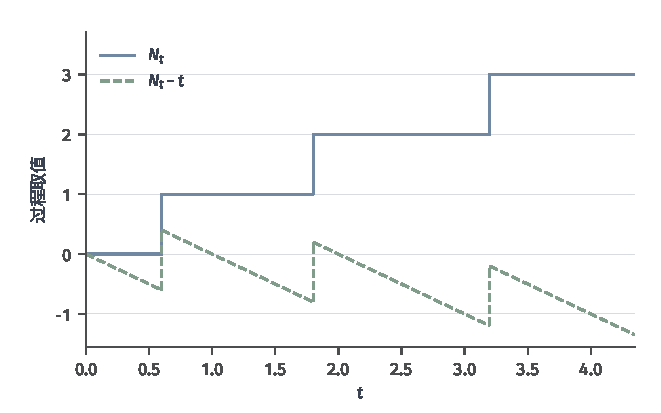
\includegraphics[width=\linewidth]{figures/00-shared/mathematical-preliminaries-lower/01-random-variables-distributions-and-causality/matplotlib/rv-poisson-compensation/figure.pdf}
  \caption{给定三次到达时刻的教学路径，取\(\lambda=1\)。蓝线为计数\(N_t\)，绿虚线为\(\widetilde N_t=N_t-t\)；两条路径在同一时刻跳跃且跳跃量相同。减去的是平均趋势，不是实现中的跳跃。}
\label{fig:rv-poisson-compensation}
\end{figure}
平方跳跃累计为
\(\sum_{s\leq t}(\Delta\widetilde N_s)^2=N_t\)，是随机量；
其可预测平均累计为\(\lambda t\)，不是同一个量。在有限活动区间上，细分路径的平方增量和趋向跳跃平方和，连续线性漂移贡献趋零，故可记
\[
[\widetilde N]_t=N_t,\qquad
\langle\widetilde N\rangle_t=\lambda t.
\]
后一个量是使\(\widetilde N_t^2-\langle\widetilde N\rangle_t\)成为鞅的可预测补偿。离散历史相关偏差中的相应定义见定义~\ref{def:stoch-predictable-quadratic-variation}。对确定分割，这个有限活动情形的路径计算可逐条进行；连续粗糙路径的二次变差将在下一例说明。

复合情形若\(\mathbb E|J_1|<\infty\)，则
\(C_t-\lambda t\,\mathbb EJ_1\)相对于只揭示已到达标记的自然历史是鞅。
若再有\(\mathbb EJ_1^2<\infty\)，其平方跳跃累计为
\(\sum_{k\leq N_t}J_k^2\)，可预测二阶累计为
\(\lambda t\,\mathbb EJ_1^2\)。例如每次损失恒为二，平均损失速率为\(2\lambda\)，二阶累计速率却为\(4\lambda\)。
随机积分将把在跳跃前确定的系数乘到这些补偿增量上；仅对有限步进系数而言，正交性已经给出
\[
\mathbb E\left(\sum_iH_i
(\widetilde N_{t_{i+1}}-\widetilde N_{t_i})\right)^2
=\lambda\sum_i\mathbb E H_i^2(t_{i+1}-t_i),
\quad H_i\in L^2(\mathcal F_{t_i}),
\]
这里使用确定分割与可预测系数。一般过程积分的定义及闭包条件见
第~\ref{chap:action-and-state}章，其中
第~\ref{sec:action-state-poisson-integral}节将把这一有限和延拓为补偿Poisson积分。

\subsection{基于高斯规律的随机过程生成}

规定多个时刻的联合高斯分布时，均值和协方差就能组织全部有限维规律。独立增量给出Brownian模型；一般协方差核则允许不同的时间依赖。有限维规律能否相容、路径能否连续，仍是两个要分别检查的问题。
\label{sec:rv-gaussian-generation}

\subsubsection{独立高斯增量下的布朗路径构造}
\label{sec:dynamical-brownian-motion}
与一次一次的跳跃相对，连续波动的每段增量可越来越小，但累计波动仍然非零。布朗运动给出这种尺度的基本模型；连续路径不等于可微路径。

\paragraph{连续路径与增量尺度}
% Baseline D:1435-1490

设$\xi_{1},\xi_{2},\ldots$独立同分布， $\mathbb{E}\xi_{i}=0$、$\operatorname{Var}
(\xi_{i})=1$。 步长为$\Delta t$时，定义随机游走增量
\[
	\Delta X_{k}=\sqrt{\Delta t}\,\xi_{k}.
\]
对网格终点$t=n\Delta t$，经过正整数$n$步后，
\[
	\operatorname{Var}\left( \sum_{k=1}^{n}\Delta X_{k}\right) = n\Delta t=t.
\]
若把增量缩放成$\Delta t\,\xi_{k}$， 方差会随$\Delta t\to0$趋零；
若不缩放，固定时间内方差会发散。
平方根尺度是让连续时间极限保留有限非零波动的尺度。

在有限方差及适当插值条件下， 函数型中心极限定理把缩放随机游走连接到\term{布朗运动}（Brownian motion）。 本章不重证该一般弱收敛定理，
而从极限所需的性质定义连续对象。

\begin{definition}[标准布朗运动]
	\label{def:dynamical-standard-brownian-motion} 实值过程$(W_{t})_{t\geq0}$称为标准布朗运动，
	若它满足：
	\begin{enumerate}
		\item $W_{0}=0$几乎必然成立；

		\item 对$0\leq t_{0}<t_{1}<\cdots<t_{n}$， 增量$W_{t_i}-W_{t_{i-1}}$相互独立；

		\item $W_{t}-W_{s}\sim\mathcal{N}(0,t-s)$，其中$0\leq s<t$；

		\item 样本路径几乎必然连续。
	\end{enumerate}
\end{definition}

当布朗运动与滤过$(\mathcal{F}_t)_{t\geq0}$共同使用时，还要求$W_t$对该滤过适应，
并且对$s<t$，增量$W_t-W_s$独立于$\mathcal{F}_s$。
定义中的独立增量只比较布朗运动自身的不同时间段；加入滤过后的条件保证积分中的“过去信息”
不能预见下一段布朗增量。

由独立增量和方差公式，
\begin{equation}
	\mathbb{E}[W_{s}W_{t}]=\min(s,t). \label{eq:dynamical-brownian-covariance}
\end{equation}
例如$s\leq t$时， $W_{t}=W_{s}+(W_{t}-W_{s})$， 后一增量与$W_{s}$独立且均值为零，
所以协方差为$\mathbb{E}W_{s}^{2}=s$。

\par\medskip\noindent\textbf{布朗运动的尺度与路径正则性}\quad
对任意$c>0$，过程
\[
	\widetilde W_{t}= c^{-1/2}W_{ct}
\]
仍是标准布朗运动。 它从零出发，增量仍独立， 并且
\[
	\widetilde W_{t}-\widetilde W_{s}\sim \mathcal{N}(0,t-s).
\]
连续性也由原路径继承。 因此两过程具有相同的有限维分布。
这就是布朗运动的尺度规律。

相对于同一滤过，\(m\)维标准Brownian运动
\(\bm W_t=(W_t^{(1)},\ldots,W_t^{(m)})^\top\)由相互独立的实值标准Brownian运动组成，并要求
\[
\bm W_t-\bm W_s\ \perp\ \mathcal F_s,\qquad
\bm W_t-\bm W_s\sim\mathcal N(\bm0,(t-s)\bm I_m).
\]
若以固定矩阵\(\bm A\)混合这些分量，增量协方差变成
\((t-s)\bm A\bm A^\top\)，不再是标准Brownian的单位协方差；低秩\(\bm A\)允许退化扩散。

\paragraph{不可微性与二次变差}
% Baseline D:1492-1542
长度为\(h\)的增量典型尺度为\(\sqrt h\)，所以差商
\[
	\frac{W_{t+h}-W_{t}}{h}
\]
的标准差为$1/\sqrt{h}$， 随$h\to0$反而发散。 严格结果表明，以概率$1$，
布朗运动的样本路径在所有时刻连续，同时在任何时刻都不可微。
因此不能把$\mathrm{d}W_{t}/\mathrm{d}t$当作普通随机函数， 再用Riemann积分处理。

把各时间段的增量平方后相加，所得随机量随分割改变。要说这列随机量趋向什么，必须先约定比较的是实现中的数值、平均误差还是整个分布；这几种极限在后面的统计推断中也会分别使用。
收敛方式回用定义~\ref{def:probability-random-convergence}。

还要描述短时增量相对于网格尺度有多大。不能用“每次取值都有限”代替余项控制：所需的是坏事件的概率能被同一常数压小。概率阶记号把这种控制与确定数列的阶区分开。
概率阶回用定义~\ref{def:statistics-probability-order}。
当网格长度用连续参数\(h\downarrow0\)表示时，同样要求对所有充分小的正\(h\)，用同一个常数控制尾概率。布朗增量除以\(\sqrt h\)后总服从标准高斯，所以增量为\(O_{\mathbb P}(\sqrt h)\)。这不是对全部路径同时成立的确定上界。

\par\medskip\noindent\textbf{布朗运动的二次变差}\quad
二次变差记录细分以后仍无法消失的平方波动。它与$\operatorname{Var}(W_t)$不同：
方差在固定时刻跨样本求平均，二次变差沿同一条路径对时间增量求和再取极限。
取$[0,t]$的一列确定分割$0=t_0<\cdots<t_n=t$，其最大区间长度趋零，并记平方增量和
\[
	Q_{n}= \sum_{i=0}^{n-1}(W_{t_{i+1}}-W_{t_i})^{2}.
\]
\begin{definition}[沿确定分割的二次变差]
\label{def:dynamical-quadratic-variation}
若连续过程沿每一列网格趋零的确定分割得到的平方增量和，在时刻$t$都依概率收敛到同一个随机变量，
这个极限记为$[X]_t$，称为该过程在$[0,t]$上的二次变差。
\end{definition}
以下计算证明标准布朗运动的极限为确定量$t$，并且收敛甚至在$L^2$中成立。
其期望为
\[
	\mathbb{E}Q_{n}= \sum_{i}(t_{i+1}-t_{i})=t.
\]
独立高斯增量还给出
\[
	\operatorname{Var}(Q_{n}) = 2\sum_{i}(t_{i+1}-t_{i})^{2}\leq 2t\max_{i}(t_{i+1}
	-t_{i}).
\]
因此网格趋零时， $Q_{n}\to t$在$L^{2}$中成立，进而依概率成立。 这称为布朗运动在$[
0,t]$上的二次变差等于$t$。

普通连续可微路径的平方增量和会趋零， 因为每个增量是$O(\Delta t)$， 平方后求和为$O
(\Delta t)$。 布朗增量是$O_{\mathbb{P}}(\sqrt{\Delta t})$， 平方后恰好是$O_{\mathbb{P}}
(\Delta t)$。 后文的Itô公式之所以保留二阶导数项， 根源就在这个非零二次变差。

图~\ref{fig:reader-brownian-quadratic-variation}用同一组细网格高斯增量形成两种分割。
平方和随分割改变，但细分后趋近的是$t$，而不是左图路径在时刻$t$的高低。
单条教学折线只能说明计算对象，依概率收敛的保证来自刚才对任意确定分割给出的方差上界。
\begin{figure*}[htbp]
  \centering
  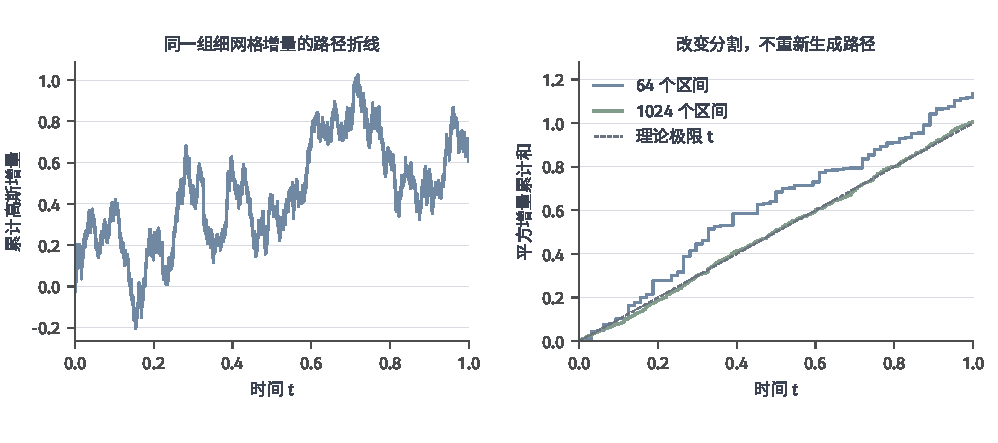
\includegraphics[width=\linewidth]{figures/00-shared/mathematical-preliminaries-lower/01-random-variables-distributions-and-causality/matplotlib/reader-brownian-quadratic-variation/figure.pdf}
  \caption{以固定随机种子构造的高斯增量教学例。左图由$4096$个独立增量
  $\Delta W_i\sim\mathcal N(0,1/4096)$累计成路径折线；右图将同一组增量分别合并为
  $64$和$1024$个时间区间，再累计各区间增量的平方。蓝、绿阶梯线使用不同分割，
  灰色参考线为理论二次变差$t$。这里只绘制有限网格，不把某一条折线作为连续布朗路径或收敛证明。}
  \label{fig:reader-brownian-quadratic-variation}
\end{figure*}

平方增量会留下有限累计量，这使普通积分的链式法则不再适用。第~\ref{chap:dynamical-systems-and-state-estimation}章将用它建立随机积分与Itô换元。
差商在固定时刻的方差发散，是不可微的尺度提示，不是“几乎必然所有时刻都不可微”的完整证明；后者同时涉及不可数多个时刻，是严格路径定理。相应地，
\(W_{t+h}-W_t=O_{\mathbb P}(\sqrt h)\)不是对全部实现、全部短区间成立的统一确定性上界。

对同一确定分割，交叉二次变差使用增量乘积而非平方：
\[
[X,Y]_t=\lim_{|\pi|\to0}\sum_{[u,v]\in\pi}
(X_v-X_u)(Y_v-Y_u),
\]
这里按存在时的依概率极限理解。独立Brownian分量\(i\ne j\)的和均值为零，方差为
\(\sum_{[u,v]\in\pi}(v-u)^2\leq t|\pi|\)，所以
\([W^{(i)},W^{(j)}]_t=0\)；同一分量的计算则给出\(t\)。合写为
\([W^{(i)},W^{(j)}]_t=\delta_{ij}t\)。
在二进分割上，对任意固定容差，平方和偏离\(t\)的概率由上述方差界控制且可求和。尾部坏事件的并集概率因而趋零，说明沿这列分割，几乎每条实现最终都不再超过该容差。再取可数个递减容差，便得到逐个固定终点的几乎必然收敛。对一般网格列，这里的无条件结论是已证明的\(L^2\)及依概率收敛，不把它加强成对所有分割同时逐路径成立。

\subsubsection{均值与协方差约束下的高斯过程构造}
% Baseline S:41-58
布朗运动已用独立高斯增量规定时间依赖。若温度曲线相隔较近时更相似，却不满足独立增量，就不能照搬这项假设。可以保留任意有限组读数联合高斯的结构，改用均值函数和协方差函数指定它们的联系；索引也可以从时间扩大为一般输入位置。
\begin{definition}[高斯过程]
  \label{def:stoch-gaussian-process}
  实值随机过程\((F(x))_{x\in\mathcal X}\)称为\term{高斯过程}（Gaussian process），若任意正整数\(m\)及任意\(x_1,\ldots,x_m\in\mathcal X\)上的向量
  \((F(x_1),\ldots,F(x_m))^\top\)均服从多元高斯分布，允许协方差奇异。其均值函数和协方差函数为
  \[
    m(x)=\mathbb E F(x),\qquad
    k(x,x')=\operatorname{Cov}(F(x),F(x')),
  \]
  因而每个有限向量的均值为\((m(x_i))_i\)，协方差矩阵为\((k(x_i,x_j))_{i,j}\)，记作\(F\sim\mathcal{GP}(m,k)\)。索引\(x\)不必代表时间。
\end{definition}
协方差函数必须对称，且对任意有限输入和实系数\(c_i\)满足
\[
  \sum_{i,j}c_ic_jk(x_i,x_j)\geq0.
\]
这正是有限协方差矩阵半正定的条件。均值与协方差因此确定高斯过程的全部有限维分布；它们本身不自动保证样本函数连续、可微或具有Markov性。

例如令\(A,B\)是独立标准高斯变量，定义\(F(x)=A+Bx\)。任意有限函数值都是\((A,B)\)的线性变换，所以构成高斯过程，且
\(m(x)=0\)、\(k(x,x')=1+xx'\)。三个以上不同输入的协方差矩阵可以奇异，因为这些随机值都由同两个随机系数决定。反过来，各点边缘高斯并不足够：若\(X\sim\mathcal N(0,1)\)，独立符号\(S\)等概率取\(\pm1\)，则\(X,SX\)的边缘均为标准高斯且不相关，但\((SX)^2=X^2\)使它们依赖，故不可能是联合高斯。定义中的“任意有限联合分布”不可省略。
布朗运动是均值零、核\(k(s,t)=\min(s,t)\)的高斯过程：每个有限向量都由独立高斯增量线性组合得到。这个核确实半正定，因为
\[
\sum_{i,j}c_ic_j\min(t_i,t_j)
=\int_0^\infty\left(\sum_i c_i\mathbb I_{\{u\leq t_i\}}\right)^2\,\mathrm du\geq0.
\]
一般给定均值和对称半正定核时，相应高斯有限维分布相容，可用第~\ref{sec:rv-finite-dimensional-laws}节的扩张定理建立过程。要得到连续版本，仍须对核控制增量矩；“高斯过程”这个名称本身不承诺路径光滑。


\subsection{基于Dirichlet规律的随机概率测度生成}
\label{sec:stoch-random-probability-generation}
\BookSectionRef{sec:rv-random-generation}{第~\ref{sec:rv-random-generation}节}的层次模型让一个参数向量随机；现在把随机对象扩大为整张概率测度。它也可以看成以可测集合为索引的一族随机质量，但每条实现还须对这些集合满足可数可加性。
把空间划成有限个区域后，一个随机分布先表现为各区域的随机概率，且这些概率之和为$1$。
有限Dirichlet分布正好描述这样的概率向量。要求任意有限分割都具有彼此相容的Dirichlet
概率向量，就得到\term{Dirichlet过程}；这里增加的是随机对象的范围，而不是直接把向量维数写成无穷。
\paragraph{随机概率测度的有限分割表示}
\begin{definition}[随机概率测度]
  \label{def:probability-random-probability-measure}
在可测空间
\((\mathcal X,\mathcal A)\)上，先给概率测度空间\(\mathcal P(\mathcal X)\)配备
\term{评价$\sigma$代数}：它由全部映射
\(\mu\mapsto\mu(A)\)，\(A\in\mathcal A\)，生成。随机概率测度就是从底层概率空间到
这个可测空间的可测映射；换言之，对每个\(A\in\mathcal A\)，\(G(A)\)都必须是随机
变量。
\end{definition}
\paragraph{相容分割下的Dirichlet过程}
\begin{definition}[Dirichlet过程]
  \label{def:probability-dirichlet-process}
  设\((\mathcal X,\mathcal A)\)为标准Borel空间，\(G_0\)为其上的概率测度，\(\alpha>0\)。随机概率测度\(G\)称为参数\((\alpha,G_0)\)的Dirichlet过程，记作\(G\sim\operatorname{DP}(\alpha,G_0)\)，若对任意有限可测分割
\((A_1,\ldots,A_K)\)，
\[ (G(A_1),\ldots,G(A_K))
  \sim\operatorname{Dirichlet}(\alpha G_0(A_1),\ldots,\alpha G_0(A_K)). \]
其中\(\alpha>0\)是总质量参数，\(G_0\)是基概率测度；若
\(G_0(A_k)=0\)，则相应坐标满足\(G(A_k)=0\)几乎必然，应删除该零参数坐标后理解Dirichlet向量。
\end{definition}
这一定义通过全部有限分割刻画随机分布。合并两个分块时，概率质量相加，Dirichlet参数也相加；这说明不同分割规律彼此相容。
相容性还不足以保证每条实现都可数可加。标准Borel空间上的存在性可由随机离散测度构造证明：Ferguson把一族正的随机跳跃质量归一化，使权重和为\(1\)，再把这些权重放在独立、服从\(G_0\)的随机位置上。所得对象逐条实现都是概率测度，各有限分割质量又满足上述Dirichlet规律\scite{statistics-ferguson1973dirichlet}。
后验、聚类表示及非参数Bayes计算留给概率模型章节。

\section{随机累计量的偏差控制}
\label{sec:probability-averages-errors}
\label{sec:rv-aggregation}
用\(n\)次读数求和或取平均后，还需要判断结果偏离目标多少。我们固定\(n\)和误差阈值，控制超出阈值的概率。
控制的对象不同，所需的论证也不同：查询一个预先固定的累计量，只需保证这一个量；
从候选族中挑出累计量最小的一个，则必须让保证同时覆盖全部候选，否则选出的那个恰好
是被噪声压低的可能性没有被排除；根据历史继续收集记录，样本量与观测时刻本身也是随机的，
条件化要求随之改变。本节依次处理这三种情形。下一节再用累计量的概率保证分析采样积分。
样本数增长后的极限不能代替当前预算下的概率界。

\subsection{单个累计量的偏差控制}
\label{sec:probability-basic-tail-bounds}
\label{sec:probability-concentration-inequalities}
\subsubsection{矩条件下的尾概率控制}
固定独立样本数后，最直接的误差指标是样本平均的方差。若\(X_1,\ldots,X_n\)相互独立，且各项二阶矩有限，记\(\overline X_n=n^{-1}\sum_{i=1}^nX_i\)，则
\[
 \operatorname{Var}(\overline X_n)
 =\frac1{n^2}\sum_{i=1}^n\operatorname{Var}(X_i).
\]
\BookSectionRef{sec:rv-features}{第~\ref{sec:rv-features}节}的Markov与Chebyshev不等式将一阶或二阶矩转成尾概率。将\BookEquationRef{eq:probability-chebyshev-inequality}{式~\eqref{eq:probability-chebyshev-inequality}}用于这里的平均误差，得到
\[
 \mathbb P\{|\overline X_n-\mathbb E\overline X_n|\geq\varepsilon\}
 \leq\frac{\sum_i\operatorname{Var}(X_i)}{n^2\varepsilon^2},
 \qquad\varepsilon>0.
\]
同分布且单次方差为\(\sigma^2\)时，右侧为\(\sigma^2/(n\varepsilon^2)\)。这个界只利用方差；相同方差的有界变量与重尾变量可能有不同的实际尾部。若样本相关，平均方差中还要保留所有交叉协方差，不能继续把方差除以\(n\)作为通用结论。

% Baseline P:1698-1841
\subsubsection{指数矩条件下的累计偏差控制}
对任意\(\lambda>0\)，函数\(x\mapsto e^{\lambda x}\)单调。Markov不等式给出
\begin{equation}
  \mathbb{P}(X\geq t)
  =
  \mathbb{P}(e^{\lambda X}\geq e^{\lambda t})
  \leq
  e^{-\lambda t}\mathbb{E}[e^{\lambda X}].
  \label{eq:probability-chernoff-step}
\end{equation}
随后对\(\lambda\)优化，便得到Chernoff方法。整个方法依赖相应指数矩有限；若\(\mathbb{E}e^{\lambda X}=\infty\)，式
\eqref{eq:probability-chernoff-step}虽形式上仍真，却不给出有用上界。

Chernoff方法把尾概率问题转成指数矩问题。对方差为\(\sigma^2\)的中心高斯变量，指数矩恰为\(\exp(\lambda^2\sigma^2/2)\)；若另一变量的指数矩也不超过这个形式，同一优化就给出高斯型尾界。因此需要命名这类具有共同指数矩上界的变量，而无需假设它们本身是高斯。
\begin{definition}[次高斯变量]
  \label{def:probability-subgaussian}
对\(\sigma^2>0\)，均值为零的可积实随机变量\(X\)若满足
\[ \mathbb{E}[e^{\lambda X}]
  \leq\exp\left(\frac{\lambda^2\sigma^2}{2}\right),\qquad \lambda\in\mathbb{R}, \]
就称它为参数\(\sigma^2\)的\term{次高斯变量}（sub-Gaussian random variable）。
\end{definition}
对\(t>0\)，代入Chernoff界并取\(\lambda=t/\sigma^2\)，得到
\[ \mathbb{P}(X\geq t)
  \leq\exp\left(-\frac{t^2}{2\sigma^2}\right). \]
“次高斯”描述的是指数矩或尾部上界，不表示变量本身服从高斯分布。

\par\medskip\noindent\textbf{有界变量的Hoeffding不等式}\quad
实际读数可能只知道上下界，尚不知道矩母函数。要继续使用Chernoff方法，就需先从区间长度推出统一的指数矩上界。Hoeffding引理完成这一步，再由独立性把单个变量的控制合成为累计量的控制。
\begin{lemma}[Hoeffding引理]
\label{lem:probability-hoeffding-lemma}
若\(\mathbb{E}X=0\)且\(X\in[a,b]\)几乎处处成立，则
\[ \mathbb{E}[e^{\lambda X}]
  \leq\exp\left\{\frac{\lambda^2(b-a)^2}{8}\right\},\qquad \lambda\in\mathbb{R}. \]
\end{lemma}

\begin{proof}
若\(a=b\)，均值为零迫使\(X=0\)，结论直接成立。以下设\(a<b\)。
凸性说明，对\(x\in[a,b]\)，指数函数位于连接端点的弦下方：
\[ e^{\lambda x}
  \leq\frac{b-x}{b-a}e^{\lambda a}+\frac{x-a}{b-a}e^{\lambda b}. \]
取期望并使用\(\mathbb{E}X=0\)。令\(p=-a/(b-a)\in[0,1]\)、
\(s=\lambda(b-a)\)，则右侧的对数为
\[
 \psi(s)=\log\bigl[(1-p)e^{-ps}+pe^{(1-p)s}\bigr].
\]
这里对无量纲变量\(s\)求导。写
\(r_s=pe^s/(1-p+pe^s)\)，直接求导得到
\(\psi''(s)=r_s(1-r_s)\leq1/4\)，且\(\psi(0)=\psi'(0)=0\)。
Taylor积分余项给出
\(\psi(s)=s^2\int_0^1(1-u)\psi''(us)\,\mathrm du\leq s^2/8\)，
对正负\(s\)都成立。代回原变量，便有
\[ \log\mathbb{E}[e^{\lambda X}]
  \leq\frac{\lambda^2(b-a)^2}{8}. \]
指数化即得结论。
\end{proof}

\begin{theorem}[Hoeffding不等式]
\label{thm:probability-hoeffding-inequality}
设\(X_1,\ldots,X_n\)相互独立，且\(X_i\in[a_i,b_i]\)几乎处处成立。若\(\sum_i(b_i-a_i)^2>0\)，则对\(t>0\)，
\[
  \mathbb{P}\left(
    \sum_{i=1}^{n}(X_i-\mathbb{E}X_i)\geq t
  \right)
  \leq
  \exp\left\{
    -\frac{2t^2}{\sum_{i=1}^{n}(b_i-a_i)^2}
  \right\}.
\]
当全部区间宽度为零时，中心化和恒为零，上述右尾概率为零。
\end{theorem}

\begin{proof}
只需证明总区间宽度平方和为正的情形。记\(S=\sum_i(X_i-\mathbb{E}X_i)\)。对\(\lambda>0\)，独立性使指数矩分解：
\[
\begin{aligned}
  \mathbb{P}(S\geq t)
  &\leq
  e^{-\lambda t}\mathbb{E}[e^{\lambda S}]\\
  &=
  e^{-\lambda t}
  \prod_{i=1}^{n}
  \mathbb{E}\left[
    e^{\lambda(X_i-\mathbb{E}X_i)}
  \right]\\
  &\leq
  \exp\left\{
    -\lambda t+
    \frac{\lambda^2}{8}
    \sum_{i=1}^{n}(b_i-a_i)^2
  \right\}.
\end{aligned}
\]
右侧关于\(\lambda\)的最小点为
\[ \lambda^\star
  =\frac{4t}{\sum_i(b_i-a_i)^2}. \]
代回即得结论。对\(-S\)使用同一结果，再用联合界可得双侧版本。
\end{proof}

若\(X_i\in[0,1]\)独立，则对\(\varepsilon>0\)，样本平均满足
\[ \mathbb{P}(|\overline{X}_n-\mathbb{E}\overline{X}_n|
  \geq\varepsilon)\leq 2e^{-2n\varepsilon^2}. \]
有界性进入Hoeffding引理，独立性进入矩母函数乘积；删除任一条件都不能沿用这份证明。

\par\medskip\noindent\textbf{方差敏感的Bernstein不等式}\quad
Hoeffding界只看到取值区间。两种读数即使区间相同，一种几乎总在均值附近，另一种经常到达端点，实际累计波动也会不同。已知方差时，可以让它控制常见的小波动，再用幅值上限限制罕见的大增量；下面的分母同时保留这两种尺度。
若独立中心化变量满足\(|X_i|\leq M\)，其中\(M>0\)，并记\(v=\sum_i\mathbb{E}[X_i^2]\)，则对\(t>0\)，Bernstein不等式的一个版本为
\begin{equation}
  \mathbb{P}\left(\sum_{i=1}^{n}X_i\geq t\right)
  \leq
  \exp\left\{
    -\frac{t^2}{2(v+Mt/3)}
  \right\}.
  \label{eq:probability-bernstein-inequality}
\end{equation}
为看清两个尺度的来源，取\(0<\lambda<3/M\)。由指数级数及
\(|X_i|^k\leq M^{k-2}X_i^2\)（\(k\geq2\)），有
\[
  \mathbb{E}e^{\lambda X_i}
  \leq
  1+\frac{\lambda^2\mathbb{E}X_i^2}
           {2(1-\lambda M/3)}
  \leq
  \exp\left\{
    \frac{\lambda^2\mathbb{E}X_i^2}
         {2(1-\lambda M/3)}
  \right\}.
\]
这里第一阶项因中心化而消失，常数\(1/3\)来自用几何级数控制
\[
  \sum_{k\geq3}\frac{(\lambda M)^{k-2}}{k!}.
\]
独立性使各指数矩相乘，Chernoff步骤于是给出
\[
  \mathbb{P}\left(\sum_iX_i\geq t\right)
  \leq
  \exp\left\{
    -\lambda t+\frac{\lambda^2v}
      {2(1-\lambda M/3)}
  \right\}.
\]
若\(v=0\)，则全部\(X_i=0\)几乎处处，尾概率为零。若\(v>0\)，取\(\lambda=t/(v+Mt/3)\in(0,3/M)\)便得到式~\eqref{eq:probability-bernstein-inequality}。小偏差区域由\(v\)主导，呈高斯型；大偏差区域由\(Mt\)主导，呈指数型。

例如\(B_i\sim\operatorname{Bernoulli}(0.01)\)独立，考虑
\(\overline{B}_n-0.01\geq0.05\)。Hoeffding上界为
\(\exp(-0.005n)\)，而Bernstein上界约为
\[
  \exp\left\{
    -\frac{0.05^2n}
      {2(0.01\times0.99+0.05/3)}
  \right\}
  \approx \exp(-0.047n).
\]
低发生率使实际方差远小于区间最坏尺度，所以后者明显更紧；当方差接近区间允许的最大值或偏差进入线性尺度时，Bernstein并不保证处处优于Hoeffding。

对重尾变量，方差可能不存在，指数矩也可能对所有正参数发散。此时Chebyshev、Hoeffding和Bernstein各自在矩、范围或指数矩步骤失效。可以增加截断、稳健均值或仅用
有限\(p\)阶矩推导多项式尾界，但所得估计对象和偏差需要重新说明，不能继续声称高斯型集中。

\subsection{候选族累计量的统一偏差控制}
\label{sec:probability-uniform-errors-symmetry}
\label{sec:probability-random-functions-uniform-error}
设同一批记录既用于计算多个候选的平均，又要从中挑出表现最好的一个。选择规则会天然偏向那些偶然偏低的平均，所以对单个预先固定的候选成立的误差保证，未必适用于选中的候选。要让结论对选中的候选也有效，需要构造一个共同事件：在这个事件上，每个候选的累计误差都同时受控。这里上确界遍历候选函数，求和索引遍历样本；这两个范围共同决定保证的含义。

\paragraph{有限候选的联合控制}
% Baseline P:1855-1917
设有限候选类\(\mathcal{H}=\{h_1,\ldots,h_M\}\)，损失\(\ell(h,Z)\in[0,1]\)。真实风险与经验风险分别为
\[ R(h)=\mathbb{E}[\ell(h,Z)],
  \qquad\widehat{R}_n(h)=\frac{1}{n}\sum_{i=1}^{n}\ell(h,Z_i), \]
其中\(Z_1,\ldots,Z_n\)独立同分布。对预先固定的单个\(h\)，Hoeffding不等式给出
\[ \mathbb{P}\bigl(
    |\widehat{R}_n(h)-R(h)|>\varepsilon\bigr)\leq 2e^{-2n\varepsilon^2}. \]
但经验最优候选
\(\widehat{h}\in\arg\min_h\widehat{R}_n(h)\)由同一批训练样本选出，不是预先固定对象。只控制一个候选不能排除“恰好因噪声看起来最好”的选择偏差。

为明确“同时控制”与“样本量足够”的关系，把上述要求写成一个定义。这里讨论抽样前固定的函数类；所有上确界均假定可测。一项常用充分条件是存在可数子类，使每个函数都是该子类中某个序列的逐点极限。
\begin{definition}[分布无关的一致收敛]
  \label{def:uniform-convergence}
  设\(\mathcal G\)是非空的\([0,1]\)值可测函数类。若对任意\(\eta,\delta\in(0,1)\)，存在只依赖\(\mathcal G,\eta,\delta\)的整数\(n_0\)，使任意概率分布\(P\)和任意\(n\geq n_0\)的独立同分布样本\(S=(Z_1,\ldots,Z_n)\sim P^n\)均满足
  \begin{equation}
    \mathbb P_{S\sim P^n}\left\{
      \sup_{g\in\mathcal G}\left|\frac1n\sum_{i=1}^ng(Z_i)-\mathbb E_Pg\right|\leq\eta
    \right\}\geq1-\delta,
    \label{eq:uniform-convergence-definition}
  \end{equation}
  就称\(\mathcal G\)满足分布无关的\term{一致收敛}（uniform convergence）。若只要求\(P\)属于指定分布族，同一定义给出相对于该分布族的一致收敛。
\end{definition}
“函数上一致”由上确界表达，“分布无关”则要求同一个\(n_0\)适用于全部允许分布。对每个固定函数或每个固定分布分别存在的样本量，不能自动满足这两个量词。

\begin{theorem}[有限函数类的一致误差界]
\label{thm:probability-finite-class-uniform-bound}
在上述条件下，对任意\(\delta\in(0,1)\)，以至少\(1-\delta\)的概率同时对所有\(h\in\mathcal{H}\)有
\begin{equation}
  |\widehat{R}_n(h)-R(h)|
  \leq
  \sqrt{\frac{\log(2M/\delta)}{2n}}.
  \label{eq:probability-finite-class-bound}
\end{equation}
\end{theorem}

\begin{proof}
对每个\(h\)定义坏事件
\[ A_h=
  \{|\widehat{R}_n(h)-R(h)|>\varepsilon\}. \]
单函数Hoeffding界给出\(\mathbb{P}(A_h)\leq2e^{-2n\varepsilon^2}\)。由联合界，
\[ \mathbb{P}\left(\bigcup_{h\in\mathcal{H}}A_h\right)
  \leq 2M e^{-2n\varepsilon^2}. \]
令右侧等于\(\delta\)，解得\(\varepsilon=\sqrt{\log(2M/\delta)/(2n)}\)。在坏事件并集的补集上，结论对
全部候选同时成立。
\end{proof}

令\(h^\star\in\arg\min_hR(h)\)，并在式\eqref{eq:probability-finite-class-bound}成立的事件上记右侧为\(\varepsilon_n\)。则
\[
\begin{aligned}
  R(\widehat{h})
  &\leq
  \widehat{R}_n(\widehat{h})+\varepsilon_n\\
  &\leq
  \widehat{R}_n(h^\star)+\varepsilon_n\\
  &\leq
  R(h^\star)+2\varepsilon_n.
\end{aligned}
\]
第二步正是经验最优性的用途。候选数只通过\(\log M\)进入，但若候选类本身由同一批训练样本任意生成，简单地把最终数量代入\(M\)未必合法；需要把生成过程纳入统一控制对象。
例如\(M=100\)、\(n=1000\)、\(\delta=0.05\)时，式~\eqref{eq:probability-finite-class-bound}右侧约为
\[
  \sqrt{\frac{\log 4000}{2000}}\approx0.0644.
\]
这个数同时控制一百个预先固定候选，而不是给每个候选各自提供\(95\%\)保证；后一做法的联合失败概率可能远大于\(5\%\)。
% Baseline P:1974-2031

统一控制不只用于比较预测函数，也可用于同时保护一批几何查询。若把高维点随机投影到较低维，希望所有点对的距离都近似保留，就先要控制一个方向的投影长度。高斯投影的标准化平方长度是独立标准高斯平方之和，因此先建立卡方尾界，再对有限点对使用联合界。
\begin{lemma}[\(\chi^2\)变量的尾界]
  \label{lem:probability-chi-square-tail}
  若\(Z\sim\chi_k^2\)，其中\(k\)为正整数，则对每个\(x>0\)，
  \[
    \mathbb{P}\{Z-k\geq2\sqrt{kx}+2x\}\leq e^{-x},
    \qquad
    \mathbb{P}\{k-Z\geq2\sqrt{kx}\}\leq e^{-x}.
  \]
  因而对\(0<\varepsilon<1\)，
  \begin{equation}
    \mathbb{P}\left(
      \left|\frac{Z}{k}-1\right|>\varepsilon
    \right)
    \leq2\exp\left(-\frac{k\varepsilon^2}{8}\right).
    \label{eq:probability-chi-square-relative-tail}
  \end{equation}
\end{lemma}

\begin{proof}
标准高斯积分给出\(\mathbb E e^{\lambda G^2}=(1-2\lambda)^{-1/2}\)，\(\lambda<1/2\)。独立性因而给出
\[
  \log\mathbb E e^{\lambda(Z-k)}
  =\frac{k}{2}\{-2\lambda-\log(1-2\lambda)\}
  \leq\frac{k\lambda^2}{1-2\lambda},\qquad 0<\lambda<1/2.
\]
最后一步来自\(-u-\log(1-u)=\sum_{j\geq2}u^j/j\leq u^2/[2(1-u)]\)。对上尾使用Chernoff方法，取
\(\lambda=\sqrt{x}/(\sqrt{k}+2\sqrt{x})\)，便在阈值\(2\sqrt{kx}+2x\)处得到指数\(-x\)。
对下尾，用\(u-\log(1+u)\leq u^2/2\)得到
\[
  \log\mathbb E e^{-\lambda(Z-k)}\leq k\lambda^2,\qquad\lambda>0.
\]
取\(\lambda=\sqrt{x/k}\)，在阈值\(2\sqrt{kx}\)处也得到指数\(-x\)。最后取\(x=k\varepsilon^2/8\)。当\(0<\varepsilon<1\)时，两侧阈值均不超过\(k\varepsilon\)，故相对偏差事件包含于对应尾事件的并集，联合界给出式~\eqref{eq:probability-chi-square-relative-tail}。
\end{proof}

现在把单个方向的集中推广到有限点集。这一结果称为Johnson--Lindenstrauss引理：保留有限个距离所需的随机投影维数主要随点数的对数增长，而不由原始坐标数直接决定。
\begin{theorem}[高斯随机投影的距离保持]
  \label{thm:probability-johnson-lindenstrauss}
  给定抽样前固定的\(N\geq2\)个点\(\bm x_1,\ldots,\bm x_N\in\mathbb R^d\)，以及\(\varepsilon,\delta\in(0,1)\)。若\(\bm A\in\mathbb R^{k\times d}\)的元素独立服从\(\mathcal N(0,1/k)\)，且
  \[
    k\geq\frac8{\varepsilon^2}\log\frac{N(N-1)}\delta,
  \]
  则以至少\(1-\delta\)的概率，对全部\(i,j\)同时有
  \begin{equation}
    (1-\varepsilon)\|\bm x_i-\bm x_j\|_2^2
    \leq\|\bm A\bm x_i-\bm A\bm x_j\|_2^2
    \leq(1+\varepsilon)\|\bm x_i-\bm x_j\|_2^2.
    \label{eq:probability-jl-distance-preservation}
  \end{equation}
\end{theorem}
\begin{proof}
固定一个不依赖\(\bm A\)的非零向量\(\bm v\)。矩阵各行独立，每个\((\bm A\bm v)_r\)均为均值零、方差\(\|\bm v\|_2^2/k\)的高斯变量，因此
\[
  \frac{k\|\bm A\bm v\|_2^2}{\|\bm v\|_2^2}\sim\chi_k^2.
\]
引理~\ref{lem:probability-chi-square-tail}使该方向的相对平方范数失真概率不超过\(2e^{-k\varepsilon^2/8}\)。点对差至多有\(N(N-1)/2\)个；对全部非零差使用联合界，失败概率不超过\(N(N-1)e^{-k\varepsilon^2/8}\leq\delta\)。零差经任何线性投影仍为零，无须额外尾界。
\end{proof}
结论控制的是平方距离；对距离本身开方后，因子为\(\sqrt{1\pm\varepsilon}\)。点集须在投影抽样前确定，但在同时保持事件上，可以事后任选这批点中的一对查询。它不保证对观察到\(\bm A\)后任意新造的向量都保持范数；当\(k<d\)时，\(\bm A\)的非零零空间方向就给出反例。这里的常数是便于推导的充分界，也不保证所得\(k\)一定小于\(d\)。

\paragraph{无限候选的统一控制}
% Baseline P:1921-1961
无限函数类不能直接按元素做联合界。样本上的有限取值模式与覆盖网中的有限代表，提供两种有限化方法。
使用样本取值模式时，须先引入独立样本副本并进行下文的对称化，再条件于两批合并样本。此时随机符号和只由样本上的有限取值模式决定，才可对模式使用条件尾界和联合界；这一有限计数须在条件化以后进行。
同一个样本模式可能对应不同的真实风险，因此不能直接把前面固定候选界中的\(M\)换成当前样本的模式数。
使用覆盖网时，若每个函数都能由有限\(\varepsilon\)-网中的代表逼近，则先控制网点，再用Lipschitz性质把误差转回原函数。下面先建立后一种方法所需的误差比较，再说明对称化怎样引入随机符号。

\begin{lemma}[覆盖数的有限网控制]
  \label{lem:probability-covering-finite-net}
  设\((\mathcal{F},d)\)具有有限\(\varepsilon\)-网
  \(\mathcal{N}_\varepsilon\)，其大小为
  \(N(\mathcal{F},d,\varepsilon)\)。若随机过程
  \(\{Z_f:f\in\mathcal{F}\}\)满足
  \[
    |Z_f-Z_g|\leq Ld(f,g)
  \]
  几乎处处对所有\(f,g\)成立，并且相关上确界可测，则对任意\(t>0\)，
  \begin{equation}
    \mathbb{P}\left\{
      \sup_{f\in\mathcal{F}}|Z_f|>t+L\varepsilon
    \right\}
    \leq
    N(\mathcal{F},d,\varepsilon)
    \sup_{f\in\mathcal{F}}\mathbb{P}(|Z_f|>t).
    \label{eq:probability-covering-finite-net}
  \end{equation}
\end{lemma}

\begin{proof}
对每个\(f\)选取满足\(d(f,g_f)\leq\varepsilon\)的
\(g_f\in\mathcal{N}_\varepsilon\)。则
\[
  |Z_f|\leq |Z_{g_f}|+L\varepsilon,
\]
所以左侧坏事件包含在
\(\bigcup_{g\in\mathcal{N}_\varepsilon}\{|Z_g|>t\}\)中。对这个有限并集使用联合界
即得结论。
\end{proof}

若\(Z_f=\widehat R_n(f)-R(f)\)，且经验风险与真实风险各自关于\(d\)都是
\(L_0\)-Lipschitz，则引理中的过程常数是\(2L_0\)。因此，网格大小、离散误差
\(2L_0\varepsilon\)和单点尾界必须一起进入结论；只报告覆盖数而不验证Lipschitz传递
还不能控制原函数类。

% Baseline P:2035-2049
有些目标不是单个样本平均，而是整批记录的函数\(F(Z_1,\ldots,Z_n)\)。若替换第\(i\)个输入最多改变\(c_i\)，即
\[ \sup_{\bm{z},z_i'}
  |F(z_1,\ldots,z_i,\ldots,z_n)-F(z_1,\ldots,z_i',\ldots,z_n)|\leq c_i, \]
当\(\sum_i c_i^2>0\)时，对\(t>0\)，独立输入下的McDiarmid不等式给出
\begin{equation}
  \mathbb{P}\bigl(
    F-\mathbb{E}F\geq t
  \bigr)
  \leq
  \exp\left\{
    -\frac{2t^2}{\sum_{i=1}^{n}c_i^2}
  \right\}.
  \label{eq:probability-mcdiarmid}
\end{equation}
若全部\(c_i=0\)，则\(F\)在样本取值的乘积域上恒定，中心化后的正尾概率为零。其证明把\(F\)依次对前\(i\)个观测条件化，形成Doob鞅；每步有界差控制一个鞅增量，再使用Hoeffding型指数矩界。独立性保证逐步揭示观测时的条件结构，有界差则限制单个观测的影响。
McDiarmid不等式的完整证明见第~\ref{sec:rv-fixed-time}节：在那里把数据函数逐步揭示为Doob鞅，并说明独立输入为什么给出所需的条件范围。
% Baseline P:2053-2272
有限候选可按数量控制误差；无限类的函数在同一组观测上可能高度相似，直接计数会忽略这种结构。\term{Rademacher复杂度}提供另一种衡量方式：固定观测点后，让函数尽量对齐一组无信号的随机正负号，再对这些正负号平均。能拟合更多随机起伏的类，需要更大的同时误差代价。
\begin{definition}[经验Rademacher复杂度]
  \label{def:rademacher-complexity}
  给定非空实值可测函数类\(\mathcal G\)和样本\(S=(z_1,\ldots,z_n)\)。令\(\sigma_i\)独立且等概率取\(-1,1\)。当上确界可测且期望有限时，\term{经验Rademacher复杂度}定义为
  \begin{equation}
    \widehat{\mathfrak R}_S(\mathcal G)
    =\mathbb E_\sigma\left[\sup_{g\in\mathcal G}\frac1n\sum_{i=1}^n\sigma_i g(z_i)\right].
    \label{eq:empirical-rademacher}
  \end{equation}
\end{definition}
固定的是样本，不是使随机和最大的函数；每一组符号都允许选择不同函数。交换上确界与期望会把所有固定函数的零均值随机和平均成零，丢掉所要衡量的拟合能力。
\begin{definition}[期望Rademacher复杂度]
  \label{def:expected-rademacher-complexity}
  对\(S\sim P^n\)，\term{期望Rademacher复杂度}定义为
  \[
    \mathfrak R_n(\mathcal G)=\mathbb E_{S\sim P^n}\widehat{\mathfrak R}_S(\mathcal G).
  \]
\end{definition}
期望复杂度还平均了抽样结果，故依赖\(P\)；经验复杂度仅依赖给定样本上的函数取值。
允许函数作凸组合会增加候选函数，却未必增加它们对随机符号的最大对齐能力。
原因在于，固定符号后，经验随机和是函数取值的线性泛函：若一个组合的各项都不超过
同一个上界，非负且归一化的加权平均也不能超过它。下面把这一几何性质写成复杂度恒等式。

\begin{theorem}[凸组合的Rademacher复杂度]
\label{thm:ensemble-convex-hull}
设$S=(z_1,\ldots,z_n)$为固定样本，$n\geq1$，$\mathcal B$为非空实值可测函数类，
且在这组样本上统一有界，即存在有限$M$使$|h(z_i)|\leq M$对所有
$h\in\mathcal B$和$i$成立。令
\[
 \operatorname{conv}(\mathcal B)
 =\left\{\sum_{t=1}^T a_t h_t:
 T\geq1,\ h_t\in\mathcal B,\ a_t\geq0,\ \sum_{t=1}^T a_t=1\right\}
\]
为全部有限凸组合构成的函数类。则
\[
 \widehat{\mathfrak R}_S(\operatorname{conv}(\mathcal B))
 =\widehat{\mathfrak R}_S(\mathcal B).
\]
若样本再按$P^n$抽取，几乎必然满足上述样本有界条件，且相应样本上确界可测、期望有限，
则期望Rademacher复杂度也满足同一恒等式。
\end{theorem}

\begin{proof}
固定一组符号$\bm\sigma$。对任意有限凸组合，由$a_t\geq0$和$\sum_ta_t=1$，
\[
 \begin{aligned}
 \frac1n\sum_{i=1}^n\sigma_i\sum_{t=1}^T a_t h_t(z_i)
 &=\sum_{t=1}^T a_t
    \left(\frac1n\sum_{i=1}^n\sigma_i h_t(z_i)\right)\\
 &\leq\sup_{h\in\mathcal B}\frac1n\sum_{i=1}^n\sigma_i h(z_i).
 \end{aligned}
\]
因此凸包上的上确界不超过基类上的上确界。反向不等式来自
$\mathcal B\subseteq\operatorname{conv}(\mathcal B)$：取$T=1$即可得到任意基函数。
于是每一组符号下的两个上确界都相等。样本上的统一有界性保证随机和与其上确界有限，
对$\bm\sigma$取期望便得经验复杂度恒等式；在额外的抽样可测性与可积条件下，再对$S$
取期望即得期望复杂度结论。证明不要求函数类有限，也不要求上确界由某个函数达到。
\end{proof}

例如，只含常值函数$0$和$1$的基类，其凸包包含全部常值$c\in[0,1]$。
固定一个观测点时，正号下的最大随机和为$1$，负号下为$0$，两类的经验复杂度都为
$1/2$。候选函数从两个增加到无穷多个，但线性随机和的最坏值仍由端点决定。
这一定理只控制实值函数的随机线性和；把组合再作阈值化等非线性变换后，
需要另外分析变换后的函数类。非负性与归一化也是凸组合的条件，不能用同一等式处理
任意符号或任意尺度的线性组合。

随机符号只改变每个观测的正负方向。若还想用连续变化的随机幅度探测同一组函数取值，可以把符号换成标准高斯系数。它仍衡量函数类对无信号随机起伏的拟合能力，但随机探测规律变了，所得复杂度需单独定义。
\begin{definition}[经验高斯复杂度]
  \label{def:gaussian-complexity}
  将随机符号换成独立标准高斯系数\(\xi_i\sim\mathcal N(0,1)\)，定义
  \[
    \widehat{\mathfrak G}_S(\mathcal G)
    =\mathbb E_\xi\left[\sup_{g\in\mathcal G}\frac1n\sum_{i=1}^n\xi_i g(z_i)\right].
  \]
  相应期望高斯复杂度为\(\mathfrak G_n(\mathcal G)=\mathbb E_S\widehat{\mathfrak G}_S(\mathcal G)\)。
\end{definition}
高斯系数的符号与幅度都变化，Rademacher系数只有符号变化。二者是关于函数类的随机平均，不能按某一组系数的最大值直接比较。

双侧误差的证明常使用带绝对值版本
\[
  \widehat{\mathfrak R}^{\mathrm{abs}}_S(\mathcal G)
  =\mathbb E_\sigma\sup_{g\in\mathcal G}\left|\frac1n\sum_i\sigma_i g(z_i)\right|
  =\widehat{\mathfrak R}_S(\mathcal G\cup(-\mathcal G)),
\]
高斯版本同样定义。若\(\mathcal G=-\mathcal G\)，两种约定可直接等同；一般函数类则不能自动等同。例如只含常数函数\(g\equiv1\)的类，其不带绝对值复杂度为\(0\)；带绝对值复杂度为\(n^{-1}\mathbb E|\sum_i\sigma_i|>0\)。以下对称化沿用带绝对值约定，后续应用单侧风险界时应核对所用版本。

\par\medskip\noindent\textbf{对称化与随机函数复杂度}\quad
这些随机和怎样控制含有未知总体期望的误差？先用独立的第二批样本替代总体期望，得到两批样本平均的差；再利用每对样本交换后规律不变，引入随机正负号。对称化的作用是把未知总体量接到前面已经定义的随机函数复杂度上。
设\(\mathcal{F}\)是一族取值于\([-1,1]\)的函数，定义
\[ \Delta(\bm{Z})
  =\sup_{f\in\mathcal{F}}\left|\mathbb{E}f(Z)-\frac{1}{n}\sum_{i=1}^{n}f(Z_i)\right|. \]
引入独立同分布副本\(Z_1',\ldots,Z_n'\)。Jensen不等式给出
\[
\begin{aligned}
  \mathbb{E}_{\bm{Z}}\Delta(\bm{Z})
  &\leq
  \mathbb{E}_{\bm{Z},\bm{Z}'}
  \sup_{f\in\mathcal{F}}
  \left|
    \frac{1}{n}\sum_{i=1}^{n}
    \bigl(f(Z_i')-f(Z_i)\bigr)
  \right|.
\end{aligned}
\]
由于每对\((Z_i,Z_i')\)交换后联合分布不变，引入独立Rademacher符号\(\sigma_i\in\{-1,1\}\)不会改变差的联合分布。因此
\[
  \mathbb{E}\Delta(\bm{Z})
  \leq
  2\mathbb{E}_{\bm{Z},\bm{\sigma}}
  \sup_{f\in\mathcal{F}}
  \left|
    \frac{1}{n}\sum_{i=1}^{n}\sigma_i f(Z_i)
  \right|.
\]
右侧是带绝对值的经验Rademacher复杂度对样本取期望后的两倍。它只在观测点上考察函数类与随机符号对齐的能力，把未知总体期望转成了条件于样本的随机和。

若\(\phi_i:\mathbb{R}\to\mathbb{R}\)均为\(L\)-Lipschitz且\(\phi_i(0)=0\)，则对任意不必关于取负封闭的函数类\(\mathcal{F}\)，带绝对值的收缩不等式为
\[
  \mathbb{E}_{\bm{\sigma}}
  \sup_{f\in\mathcal{F}}
  \left|
    \sum_i\sigma_i\phi_i(f(Z_i))
  \right|
  \leq
  2L\,
  \mathbb{E}_{\bm{\sigma}}
  \sup_{f\in\mathcal{F}}
  \left|
    \sum_i\sigma_i f(Z_i)
  \right|.
\]
一般情形需要先在取值向量类中临时加入零向量，再分别控制随机和的两个方向；这一步产生因子\(2\)。若变换后的取值向量类关于取负封闭，例如
\(\mathcal{F}=-\mathcal{F}\)且每个\(\phi_i\)都是奇函数，则可去掉该因子。这个不等式允许把预测函数的复杂度传到Lipschitz损失。若损失不全局Lipschitz或相关上确界不可积，必须限制作用范围或使用其他矩条件。

标量收缩可用逐坐标替换证明。先设函数类在固定样本上的取值向量组成有限集
\(\mathcal{A}\subset\mathbb{R}^n\)，并只考虑不带绝对值的上确界。固定前
\(n-1\)个符号，把相应部分记为\(U_{\bm{a}}\)。条件于这些符号，左侧最后一个坐标的贡献为
\[
  \frac12\sup_{\bm{a}}\{U_{\bm{a}}+\phi_n(a_n)\}
  +\frac12\sup_{\bm{a}}\{U_{\bm{a}}-\phi_n(a_n)\}.
\]
取两个上确界的近似最大元\(\bm{a},\bm{b}\)，并使用
\(\phi_n(a_n)-\phi_n(b_n)\leq L|a_n-b_n|\)。按
\(a_n-b_n\)的符号选择正负方向，便得到上式不超过
\[
  \frac12\sup_{\bm{a}}\{U_{\bm{a}}+La_n\}
  +\frac12\sup_{\bm{a}}\{U_{\bm{a}}-La_n\}.
\]
从最后一个坐标向前迭代，即得到单侧收缩。对随机和的正、负两个方向分别应用该结论，再用
\(\sup|S|=\max\{\sup S,\sup(-S)\}\)时，还需要保证两个单侧上确界非负。具体地，令
\(\mathcal{A}_0=\mathcal{A}\cup\{\bm{0}\}\)。由于\(\phi_i(0)=0\)，对每组固定符号都有
\[
\begin{aligned}
  \sup_{\bm{a}\in\mathcal{A}}
  \left|\sum_i\sigma_i\phi_i(a_i)\right|
  &\leq
  \sup_{\bm{a}\in\mathcal{A}_0}
  \sum_i\sigma_i\phi_i(a_i)
  +
  \sup_{\bm{a}\in\mathcal{A}_0}
  \left(-\sum_i\sigma_i\phi_i(a_i)\right).
\end{aligned}
\]
两个单侧上确界因包含零向量而非负。分别对\(\bm{\sigma}\)与\(-\bm{\sigma}\)应用单侧收缩，再利用二者同分布，得到
\[
  \mathbb{E}_{\bm{\sigma}}
  \sup_{\bm{a}\in\mathcal{A}}
  \left|\sum_i\sigma_i\phi_i(a_i)\right|
  \leq
  2L\,
  \mathbb{E}_{\bm{\sigma}}
  \sup_{\bm{a}\in\mathcal{A}_0}
  \sum_i\sigma_i a_i
  \leq
  2L\,
  \mathbb{E}_{\bm{\sigma}}
  \sup_{\bm{a}\in\mathcal{A}}
  \left|\sum_i\sigma_i a_i\right|.
\]
这就闭合了带绝对值版本的证明。一般函数类可由有限子类逼近并使用单调极限；不可数类还须保留前述可测性条件。

线性函数类展示了这一复杂度怎样落到熟悉的范数上。设
\[
  \mathcal{F}
  =\{\,\bm{z}\mapsto\langle\bm{w},\bm{z}\rangle:
       \lVert\bm{w}\rVert_2\leq B\,\},
  \qquad \lVert\bm{Z}_i\rVert_2\leq R.
\]
由对偶范数和Jensen不等式，
\[
\begin{aligned}
  \widehat{\mathfrak{R}}_{\bm{Z}}^{\mathrm{abs}}(\mathcal{F})
  &=
  \frac{B}{n}\mathbb{E}_{\bm{\sigma}}
  \left\lVert\sum_{i=1}^{n}\sigma_i\bm{Z}_i\right\rVert_2\\
  &\leq
  \frac{B}{n}
  \left(\sum_{i=1}^{n}\lVert\bm{Z}_i\rVert_2^2\right)^{1/2}
  \leq\frac{BR}{\sqrt n}.
\end{aligned}
\]
参数范数、样本范数和样本量分别进入\(B\)、\(R\)与\(n^{-1/2}\)。机器学习理论部分会在具体损失和模型类上继续把这一期望复杂度转换为高概率泛化界。

把Rademacher符号替换为独立标准高斯变量\(g_i\)，得到高斯复杂度
\[ \mathbb{E}_{\bm{g}}
  \sup_{f\in\mathcal{F}}
  \left|\frac{1}{n}\sum_i g_i f(Z_i)\right|. \]
记上述带绝对值的经验Rademacher复杂度和高斯复杂度分别为
\(\widehat{\mathfrak{R}}_{\bm{Z}}^{\mathrm{abs}}(\mathcal{F})\)与
\(\widehat{\mathfrak{G}}_{\bm{Z}}^{\mathrm{abs}}(\mathcal{F})\)。对任意固定样本，只要这些上确界可测且期望有限，就有单向比较
\[
  \widehat{\mathfrak{R}}_{\bm{Z}}^{\mathrm{abs}}(\mathcal{F})
  \leq
  \sqrt{\frac{\pi}{2}}\,
  \widehat{\mathfrak{G}}_{\bm{Z}}^{\mathrm{abs}}(\mathcal{F}).
\]
这个方向可直接由条件Jensen不等式解释：写\(g_i=\sigma_i|g_i|\)，符号与幅度独立，且\(\mathbb E|g_i|=\sqrt{2/\pi}\)。固定符号后，随机和的绝对值上确界是幅度向量的凸函数，先对幅度平均不大于先取上确界再平均，因而\(\widehat{\mathfrak G}^{\mathrm{abs}}_S\geq\sqrt{2/\pi}\,\widehat{\mathfrak R}^{\mathrm{abs}}_S\)。

反方向一般不能只付出普适常数。设函数类在固定样本上的取值向量恰为
\(\{\bm e_i,-\bm e_i:1\leq i\leq n\}\)，其中\(\bm e_i\)为第\(i\)个坐标向量。两个上确界分别化为
\[
 \widehat{\mathfrak R}^{\mathrm{abs}}_{\bm Z}=\frac1n,\qquad
 \widehat{\mathfrak G}^{\mathrm{abs}}_{\bm Z}
   =\frac{\mathbb E\max_{i\leq n}|g_i|}{n}.
\]
符号的绝对值恒为\(1\)，高斯幅度的最大值却随\(n\)增长。其尺度可直接核对：
对任意\(t>0\)，指数和上界及Jensen不等式给出
\[
 \mathbb E\max_i|g_i|
 \leq\frac{\log(2n)}t+\frac t2
 \leq\sqrt{2\log(2n)}
 \quad\text{当 }t=\sqrt{2\log(2n)}.
\]
下界对\(n\geq3\)取\(u=\sqrt{\log n}\geq1\)。在高斯密度积分中只保留区间
\([u,u+1/u]\)，得到
\(\mathbb P(|g_1|\geq u)\geq c\,u^{-1}e^{-u^2/2}\)，其中\(c>0\)为固定常数。
于是独立性给出
\[
 \mathbb P(\max_i|g_i|\geq u)
 \geq1-\exp\{-cn^{1/2}/\sqrt{\log n}\}\longrightarrow1.
\]
用期望下界\(u\,\mathbb P(\max_i|g_i|\geq u)\)可知，两种复杂度的比为
\(\Theta(\sqrt{\log n})\)（\(n\geq2\)，有限个小\(n\)并入常数）。
因此替换复杂度时必须保留比较方向；这个例子已经排除了普适常数的反向界。

\subsection{历史依赖下累计量的偏差控制}

逐步采集记录时，下一次观测的位置或噪声尺度可以依赖已见历史。即使每个新增量在历史条件下均值为零，它们也未必独立，不能直接乘上独立样本的指数矩。鞅差的条件均值提供替代起点；累计条件方差则记录实际沿途产生了多少波动。
% Baseline S:427-437
\begin{definition}[可预测二次变差]
  \label{def:stoch-predictable-quadratic-variation}
对平方可积鞅差，定义\term{可预测二次变差}（predictable quadratic variation）
\begin{equation}
  V_t=\sum_{s=1}^{t}\mathbb{E}[X_s^2\mid\mathcal{F}_{s-1}].
  \label{eq:stoch-predictable-quadratic-variation}
\end{equation}
\end{definition}
它在每一步使用新增量到来之前可知的条件方差，因而能够记录实际噪声规模。与之不同，
$\sum_{s=1}^{t}X_s^2$是观察后的实现二次变差。Freedman界使用前者；在其他序贯估计中
也可以围绕后者构造界，但不能不加说明地互换。

\paragraph{固定时刻的误差界}
\label{sec:rv-fixed-time}
% Baseline S:489-540
若只知道每个鞅差的范围，可以把独立变量的指数矩方法逐步条件化。

\begin{theorem}[Azuma--Hoeffding不等式]
  \label{thm:stoch-azuma-hoeffding}
  设$(X_t,\mathcal{F}_t)_{t=1}^{n}$为鞅差，并且几乎必然有
  $a_t\leq X_t\leq b_t$，其中$a_t,b_t$为确定常数。令
  $S_n=\sum_{t=1}^{n}X_t$。若$\sum_t(b_t-a_t)^2>0$，则对任意$x>0$，
  \begin{equation}
    \mathbb{P}(S_n\geq x)\leq\exp\left\{
      -\frac{2x^2}{\sum_{t=1}^{n}(b_t-a_t)^2}
    \right\}.
    \label{eq:stoch-azuma-hoeffding}
  \end{equation}
若全部宽度为零，鞅差条件均值零使每个$X_t=0$几乎必然，正尾概率为零。
\end{theorem}

\begin{proof}
对总宽度平方和为正的情形，条件Hoeffding引理给出，对任意$\lambda>0$，
\[
  \mathbb{E}[
    \exp(\lambda X_t)
    \mid\mathcal{F}_{t-1}]
  \leq
  \exp\left\{
    \frac{\lambda^2(b_t-a_t)^2}{8}
  \right\}.
\]
从$t=n$开始反复使用塔式性质，得到
\[
  \mathbb{E}\exp(\lambda S_n)
  \leq
  \exp\left\{
    \frac{\lambda^2}{8}
    \sum_{t=1}^{n}(b_t-a_t)^2
  \right\}.
\]
Markov不等式于是给出
\[
  \mathbb{P}(S_n\geq x)
  \leq
  \exp\left\{
    -\lambda x+
    \frac{\lambda^2}{8}
    \sum_{t=1}^{n}(b_t-a_t)^2
  \right\}.
\]
对$\lambda$优化，取
$\lambda=4x/\sum_t(b_t-a_t)^2$，便得到式
\eqref{eq:stoch-azuma-hoeffding}。
\end{proof}

这个证明没有要求$X_t$彼此独立，只要求给定过去后均值为零，并且条件范围受控。代价是
它把每一步都按最坏范围计费。若多数时刻的条件方差很小，下一结果会给出更紧的尺度。
现在证明此前用于数据函数的McDiarmid界。设独立输入
\(X_1,\ldots,X_n\)，可测可积函数\(f\)在只改第\(i\)个坐标时满足
\(|f(x)-f(x')|\leq c_i\)。令
\[
Z_i=\mathbb E[f(X_1,\ldots,X_n)\mid X_1,\ldots,X_i],
\quad Z_0=\mathbb Ef,\quad D_i=Z_i-Z_{i-1}.
\]
这是逐步揭示输入的Doob鞅，且\(Z_n-Z_0=f-\mathbb Ef\)。固定已经揭示的
\(x_1,\ldots,x_{i-1}\)，把尚未揭示的输入积分掉，得到关于\(x_i\)的函数\(g_i(x_i)\)。
独立性保证这次积分使用同一未来分布，所以
\(|g_i(x_i)-g_i(x_i')|\leq c_i\)。
因此给定历史后，\(D_i\)落在长度至多\(c_i\)的区间中，并且条件均值为零。区间端点可以随历史变化，长度上界\(c_i\)则是事先固定的。
条件Hoeffding引理给出
\[
\mathbb E[e^{\lambda D_i}\mid\mathcal F_{i-1}]
\leq e^{\lambda^2c_i^2/8}.
\]
逐步取条件期望后，
\(\mathbb E e^{\lambda(f-\mathbb Ef)}
\leq e^{\lambda^2\sum_i c_i^2/8}\)。
若全部\(c_i=0\)，\(f\)为常量，结论直接成立。否则，对\(u>0\)，Chernoff优化取\(\lambda=4u/\sum_i c_i^2\)，得到
\[
\mathbb P(f-\mathbb Ef\geq u)
\leq\exp\left\{-\frac{2u^2}{\sum_i c_i^2}\right\}.
\]
对\(-f\)同样处理即得双侧界。若输入依赖，更改当前输入可能同时改变未来条件分布，上面的同一分布积分便不再成立；不能只检查\(f\)的坐标差分就套用结论。

\paragraph{任意时刻的同时误差界}
\label{sec:rv-anytime}
\label{sec:stoch-self-normalized-adaptive-design}
% Baseline S:448-485
固定轮次的误差界没有同时覆盖所有查看时刻，因而不能直接把轮次换成“第一次看起来足够好”的随机时刻。要分析这类规则，先研究停止是否保留鞅的平均关系；把停止限制在一个固定有限预算内，能够先得到一个不需要交换无穷极限的结论。
\begin{theorem}[有界停时的可选停止]
  \label{thm:stoch-bounded-optional-stopping}
  设$(M_t,\mathcal{F}_t)$为可积鞅，$\tau$为满足$\tau\leq n$几乎必然成立的停时。
  则
  \[
    \mathbb{E}[M_\tau]=\mathbb{E}[M_0].
  \]
\end{theorem}

\begin{proof}
写$X_t=M_t-M_{t-1}$。由于$\tau$为停时，事件
$\{\tau\geq t\}=\{\tau\leq t-1\}^{\mathrm{c}}$属于$\mathcal{F}_{t-1}$，故其指示
函数是可预测的。又因为$\tau\leq n$，
\[
  M_\tau
  =
  M_0+\sum_{t=1}^{n}\mathbb{I}\{\tau\geq t\}X_t.
\]
对每一项使用塔式性质与鞅差条件，
\[
  \mathbb{E}\!\left[
    \mathbb{I}\{\tau\geq t\}X_t
  \right]
  =
  \mathbb{E}\!\left[
    \mathbb{I}\{\tau\geq t\}
    \mathbb{E}[X_t\mid\mathcal{F}_{t-1}]
  \right]
  =0.
\]
有限求和后即得结论。
\end{proof}

定理的证明清楚标出了有界性用途：它把随机长度的和改写为固定的有限和。对几乎必然有限的无界停时，还需要
额外条件，例如鞅一致可积、停止后的变量由某个可积变量控制，或增量有界且
$\mathbb{E}\tau<\infty$。这些条件不能省略。对从$0$开始的公平随机游走，令
$\tau=\inf\{t:S_t=1\}$。该停时几乎必然有限，却有$S_\tau=1$，所以
$\mathbb{E}S_\tau=1\neq0$；这里$\mathbb{E}\tau=\infty$，不能套用有界停时定理。

这两个首达性质可以在有限区间中核对。对正整数\(m\)，令\(\sigma_m\)为游走首次到达\(1\)或\(-m\)的时刻。
从任一内部位置出发，接下来\(m+1\)步连续向右的概率为\(2^{-(m+1)}\)，且这会使游走离开区间。因此按长度\(m+1\)分块，未退出的概率有几何上界，保证\(\mathbb E\sigma_m<\infty\)。
从位置\(j\)开始，记到达右端的概率为\(p_j\)、退出时间期望为\(e_j\)。按第一步条件化，
\[
 p_j=\tfrac12(p_{j-1}+p_{j+1}),\qquad
 e_j=1+\tfrac12(e_{j-1}+e_{j+1}),
\]
边界为\(p_{-m}=0,p_1=1,e_{-m}=e_1=0\)。解这两个有限差分方程得到
\[
 p_j=\frac{j+m}{m+1},\qquad e_j=(j+m)(1-j).
\]
故\(\mathbb P_0(S_{\sigma_m}=1)=m/(m+1)\)，令\(m\to\infty\)便知
\(\mathbb P_0(\tau<\infty)=1\)。另一方面，\(\sigma_m\leq\tau\)，所以
\(\mathbb E_0\tau\geq\mathbb E_0\sigma_m=m\)对每个\(m\)成立，期望只能为无穷。
% Baseline S:633-641
尽管无界停止未必保留期望等式，非负超鞅仍能给出任意时刻的越界概率控制。
\term{Ville不等式}说明：若$L_t$为非负超鞅且
$\mathbb{E}L_0\leq1$，则对\(0<\delta<1\)，
\begin{equation}
  \mathbb{P}\left(\sup_{t\geq0}L_t\geq\frac1\delta\right)
  \leq\delta.
  \label{eq:stoch-ville}
\end{equation}
在上述有界停止证明中，把鞅差的条件均值零换为非正，便得到超鞅版本
\(\mathbb E L_{\tau\wedge n}\leq\mathbb E L_0\leq1\)。
固定\(0<a'<a=1/\delta\)，令\(\tau\)为首次满足\(L_t\geq a'\)的时刻。
非负性给出\(a'\mathbb P(\tau\leq n)\leq\mathbb E L_{\tau\wedge n}\leq1\)；
令\(n\to\infty\)，可知某时刻实际达到\(a'\)的概率不超过\(1/a'\)。
事件\(\{\sup_tL_t\geq a\}\)包含在每个较低阈值\(a'\)的越界事件中，再令\(a'\uparrow a\)，即得式~\eqref{eq:stoch-ville}。这样也涵盖上确界只被逼近、未在某个时刻取到的情形。
反演这类同时有效的检验，可以得到随时间更新的置信集合。
% Baseline S:544-631
Ville控制的是非负超鞅越界；要把它用于累计误差\(S_t\)，还须构造连接\(S_t\)与其条件方差\(V_t\)的指数超鞅。Freedman界沿这条路线，在同一时刻累计误差已大而方差预算尚小的事件上给出控制，比只使用增量范围多保留了实际波动信息。
\begin{theorem}[标量Freedman不等式]
  \label{thm:stoch-freedman}
  设$(X_t,\mathcal{F}_t)_{t\geq1}$为鞅差，且对某个$b>0$，有$|X_t|\leq b$几乎必然成立。
  令
  \[
    S_t=\sum_{s=1}^{t}X_s,\qquad
    V_t=\sum_{s=1}^{t}
      \mathbb{E}[X_s^2\mid\mathcal{F}_{s-1}].
  \]
  则对任意$x,v>0$，
  \begin{equation}
    \mathbb{P}\left(\exists t\geq1:S_t\geq x,\ V_t\leq v\right)
    \leq\exp\left\{
      -\frac{x^2}{2(v+bx/3)}
    \right\}.
    \label{eq:stoch-freedman}
  \end{equation}
\end{theorem}

\begin{proof}
对$0<\lambda<3/b$，标量不等式
\[
  \mathrm{e}^{\lambda u}
  \leq
  1+\lambda u+
  \frac{\lambda^2u^2}{2(1-\lambda b/3)},
  \qquad |u|\leq b,
  \]
与$\mathbb{E}[X_t\mid\mathcal{F}_{t-1}]=0$共同给出
\[
  \mathbb{E}[
    \mathrm{e}^{\lambda X_t}
    \mid\mathcal{F}_{t-1}]
  \leq
  \exp\left\{
    \psi(\lambda)
    \mathbb{E}[X_t^2\mid\mathcal{F}_{t-1}]
  \right\},
  \quad
  \psi(\lambda)=
  \frac{\lambda^2}{2(1-\lambda b/3)}.
\]
因此
\[
  L_t(\lambda)
  =
  \exp\{\lambda S_t-\psi(\lambda)V_t\},
  \qquad L_0(\lambda)=1,
\]
是非负超鞅。

令
\[
  \tau
  =
  \inf\{t\geq1:S_t\geq x,\ V_t\leq v\}.
  \]
对任意整数$n$，$\tau\wedge n$有界。对非负超鞅应用有界停时论证，
$\mathbb{E}L_{\tau\wedge n}(\lambda)\leq1$。在事件$\{\tau\leq n\}$上，
  \[
  L_\tau(\lambda)\geq\exp\{\lambda x-\psi(\lambda)v\}.
  \]
故
\[
  \mathbb{P}(\tau\leq n)\leq\exp\{-\lambda x+\psi(\lambda)v\}.
  \]
令$n\to\infty$，再取
$\lambda=x/(v+bx/3)$；该值位于$(0,3/b)$，代入后得到式
\eqref{eq:stoch-freedman}。
\end{proof}

若$X_1,\ldots,X_n$相互独立、中心化且$|X_t|\leq b$，并且
$\sum_{t=1}^{n}\operatorname{Var}(X_t)\leq v$，则自然滤过下的$X_t$构成鞅差，
且$V_n\leq v$确定成立。在式~\eqref{eq:stoch-freedman}中固定$t=n$便得到
\[
  \mathbb{P}(S_n\geq x)
  \leq
  \exp\left\{
    -\frac{x^2}{2(v+bx/3)}
  \right\}.
\]
这正是式~\eqref{eq:probability-bernstein-inequality}的同常数单侧Bernstein型界。
因此，Freedman界把独立变量的方差敏感界推广到了条件方差随历史变化的序贯情形。

Freedman界同时控制所有可能时刻，但事件中还限定了$V_t\leq v$。若希望得到随观测方差
自动变化的单一边界，可以把$V_t$的可能范围分成几何区间，对各区间使用不同$v$并分配
失败概率；更精细的方法直接混合不同$\lambda$。无论采用哪种构造，序贯有效性都来自
非负超鞅，而不是把固定时刻界中的$n$替换为随机停时。
用同一族失败事件\(E_t\)表示第\(t\)次查看时所用误差界被违反。表~\ref{tab:rv-viewing-time-guarantees}
比较时间量词：采用并合界合并逐次保证时，需要为各次查看分配失败概率。
\begin{table*}[htbp]
  \centering\small
  \begin{tabularx}{\linewidth}{p{22mm}p{39mm}XX}
    \toprule
    查看方式 & 受控事件 & 所需保证 & 可据此判断的范围\\
    \midrule
    事先固定\(n\) & \(E_n\) & \(\mathbb P(E_n)\leq\delta\) & 只控制预先指定的这一次查看；更换成历史决定的时刻需要另行证明。\\
    最多查看\(T\)次 & \(\bigcup_{t=1}^T E_t\) & 各次\(\mathbb P(E_t)\leq\delta_t\)，且\(\sum_{t=1}^T\delta_t\leq\delta\) & 并合界控制总失败概率；事件无须相互独立。\\
    任意时刻同时有效 & \(\bigcup_{t\geq1}E_t\) & \(\mathbb P(\bigcup_{t\geq1}E_t)\leq\delta\) & 对几乎必然有限的正整数停时\(\tau\)，仍有\(\mathbb P(E_\tau)\leq\delta\)。\\
    \bottomrule
  \end{tabularx}
  \caption{查看时刻变化下的误差保证。\(E_t\)须包含所用界的完整条件：例如Freedman事件同时要求
  \(S_t\geq x\)与\(V_t\leq v\)。非负超鞅可经Ville不等式构造同时界；有界可选停止的期望等式本身不提供这类失败概率保证。}
  \label{tab:rv-viewing-time-guarantees}
\end{table*}

% Baseline S:686-813
标量累计和把每次噪声视为同一个方向。在线性观测中，第$t$次查询带有特征
$\bm{x}_t\in\mathbb{R}^d$，观测为
\begin{equation}
  y_t=\langle\bm{x}_t,\bm{\theta}^{\star}\rangle+\eta_t.
  \label{eq:stoch-adaptive-linear-observation}
\end{equation}
允许$\bm{x}_t$根据$\mathcal{F}_{t-1}$中的历史结果选择，但要求它在$\eta_t$揭晓前
已经确定，也就是$\bm{x}_t$可预测；噪声$\eta_t$对$\mathcal{F}_t$可测。
\begin{definition}[条件次高斯噪声]
  \label{def:stoch-conditional-subgaussian}
对\(\mathcal F_t\)-可测实随机变量\(\eta_t\)，若某个$R>0$使下面的条件指数矩界对每个\(\gamma\in\mathbb R\)几乎必然成立，则称其相对于过去信息\(\mathcal F_{t-1}\)为参数\(R^2\)的条件次高斯噪声：
\begin{equation}
  \mathbb{E}[
    \exp(\gamma\eta_t)
    \mid\mathcal{F}_{t-1}]
  \leq
  \exp\left(\frac{\gamma^2R^2}{2}\right),
  \qquad \gamma\in\mathbb{R},
  \label{eq:stoch-conditional-subgaussian}
\end{equation}
\end{definition}
该条件蕴含可积性和给定过去后均值为零，并且尾部由尺度$R$控制。

后面还要把确定参数\(\gamma\)换成过去可测的随机参数，这一步需要可测逼近。
若\(\Gamma\)只取有限个有理值且对\(\mathcal F_{t-1}\)可测，在各取值事件上应用式~\eqref{eq:stoch-conditional-subgaussian}，得到
\[
 \mathbb E\!\left[
 e^{\Gamma\eta_t-R^2\Gamma^2/2}\mid\mathcal F_{t-1}
 \right]\leq1.
\]
对任意有限实值的\(\mathcal F_{t-1}\)-可测\(\Gamma\)，取有理值简单函数\(\Gamma_k\to\Gamma\)逐点逼近。
对每个\(A\in\mathcal F_{t-1}\)，非负Fatou引理给出
\[
 \mathbb E[\mathbb I_A e^{\Gamma\eta_t-R^2\Gamma^2/2}]
 \leq\liminf_k
 \mathbb E[\mathbb I_A e^{\Gamma_k\eta_t-R^2\Gamma_k^2/2}]
 \leq\mathbb P(A).
\]
这就验证了同一条件期望界仍成立，且避免对不可数多个参数的零测例外集取并。

取事先固定的正定矩阵\(\bm V_0\)。累计噪声和正则化设计矩阵分别记为
\begin{equation}
  \bm{S}_t=\sum_{s=1}^{t}\bm{x}_s\eta_s,
  \qquad
  \bm{V}_t=\bm{V}_0+\sum_{s=1}^{t}\bm{x}_s\bm{x}_s^{\top},
  \quad\bm{V}_0\succ\bm{0}.
  \label{eq:stoch-vector-sum-design}
\end{equation}
若各增量满足\(\mathbb E\lVert\bm x_t\eta_t\rVert_2<\infty\)，可预测性与条件中心化共同保证
\[
  \mathbb{E}[\bm{x}_t\eta_t\mid\mathcal{F}_{t-1}]
  =
  \bm{x}_t
  \mathbb{E}[\eta_t\mid\mathcal{F}_{t-1}]
  =\bm{0}.
\]
这时$(\bm{S}_t)$是向量鞅。特征可预测不自动保证这一可积性；下面的指数超鞅论证只需其条件指数矩控制，因此自归一化界不要求额外假定整个向量和可积。这里没有要求$\bm{x}_t$为确定向量，也没有要求不同
$\bm{x}_t$彼此独立；关键是它在当前噪声出现前已经由过去确定。

某个方向被反复观测时，$\bm{V}_t$沿该方向增大；从未被询问的方向只剩初始正则化。
因此，自然误差尺度不是统一的欧氏球，而是
\[
  \lVert\bm{S}_t\rVert_{\bm{V}_t^{-1}}
  =\sqrt{\bm{S}_t^{\top}\bm{V}_t^{-1}\bm{S}_t}.
\]
设计提供的信息越多，逆矩阵在相应方向上的权重越小。这种由随机设计自身归一化误差的形式，
称为\term{自归一化}（self-normalized）；它与第~\ref{sec:probability-monte-carlo-variance-reduction}节中用
随机权重和归一化分母构造的自归一化重要性估计不是同一个对象。

\par\medskip\noindent\textbf{混合指数超鞅与向量集中}\quad
\begin{theorem}[向量自归一化集中界]
  \label{thm:stoch-vector-self-normalized}
  在式~\eqref{eq:stoch-adaptive-linear-observation}至
  \eqref{eq:stoch-vector-sum-design}的条件下，对任意$\delta\in(0,1)$，以至少
  $1-\delta$的概率，对所有$t\geq0$同时有
  \begin{equation}
    \lVert\bm{S}_t\rVert_{\bm{V}_t^{-1}}
    \leq
    R\sqrt{
      2\log\left(
        \frac{\det(\bm{V}_t)^{1/2}}
             {\det(\bm{V}_0)^{1/2}\delta}
      \right)
    }.
    \label{eq:stoch-vector-self-normalized-bound}
  \end{equation}
\end{theorem}

\begin{proof}
固定任意$\bm{u}\in\mathbb{R}^d$。由于$\bm{x}_t$对
$\mathcal{F}_{t-1}$可测，在式~\eqref{eq:stoch-conditional-subgaussian}中取
$\gamma=\langle\bm{u},\bm{x}_t\rangle$，得到
\[
  \mathbb{E}\!\left[
    \exp\left\{
      \langle\bm{u},\bm{x}_t\rangle\eta_t
      -\frac{R^2}{2}
       \langle\bm{u},\bm{x}_t\rangle^2
    \right\}
    \middle|\mathcal{F}_{t-1}
  \right]
  \leq1.
  \]
逐步相乘可知
\[
  L_t(\bm{u})
  =
  \exp\left\{
    \langle\bm{u},\bm{S}_t\rangle
    -\frac{R^2}{2}
     \lVert\bm{u}\rVert_{\bm{V}_t-\bm{V}_0}^2
  \right\}
\]
是非负超鞅。

一个固定$\bm{u}$只能控制一个投影方向。为同时处理所有方向，取独立于数据的随机向量
$\bm{U}\sim\mathcal{N}(\bm{0},R^{-2}\bm{V}_0^{-1})$，并对
$L_t(\bm{U})$关于$\bm{U}$积分。非负性允许交换条件期望与积分，所以混合过程
$\overline L_t=\mathbb{E}_{\bm{U}}L_t(\bm{U})$仍是非负超鞅，且
$\overline L_0=1$。把高斯密度与指数中的二次项合并，配方得到
\begin{align*}
  \overline L_t
  &=
  \left(
    \frac{\det(\bm{V}_0)}
         {\det(\bm{V}_t)}
  \right)^{1/2}
  \exp\left\{
    \frac{1}{2R^2}
    \lVert\bm{S}_t\rVert_{\bm{V}_t^{-1}}^2
  \right\}.
\end{align*}
这里行列式比来自两个高斯二次型的归一化常数，而指数项来自配方后的中心移动。

对$\overline L_t$使用式~\eqref{eq:stoch-ville}，以至少$1-\delta$的概率，对所有$t$
都有$\overline L_t<1/\delta$。取对数并整理，便得到式
\eqref{eq:stoch-vector-self-normalized-bound}。
\end{proof}

证明中的各项假设承担不同作用。条件次高斯性构造每一步指数超鞅；特征可预测性允许在条件
期望中把$\bm{x}_t$视为已知；$\bm{V}_0\succ\bm{0}$使高斯混合与逆矩阵从$t=0$起有
定义。由高斯混合得到的行列式比则记录各方向相对于初始尺度的共同增长。行列式不是把每个访问次数简单相加，
因为同一方向的重复观测与新方向的首次观测提供的信息不同。


\section{基于随机采样的积分计算}
\label{sec:stoch-sampling-integrals}
给定概率规律和被积函数后，积分仍可能难以直接求出。采样计算把这一确定的积分目标改写成随机累计量，再用其均值、方差和尾概率检查有限预算下的误差。改变抽样分布、利用已知辅助均值、消去条件内随机性与消去归一化常数，会改变不同的计算环节。

\subsection{基于独立样本平均的积分计算}
\label{sec:probability-monte-carlo-variance-reduction}
% Baseline P:1518-1691
前面的偏差界把总体期望作为比较的参照；计算时也可能恰好不知道这个期望，而只能从给定分布抽样。此时用样本平均近似积分，就得到蒙特卡洛方法。需要分别核对平均是否对准原积分，以及相同样本预算下波动有多大。
目标积分可统一写成
\[ I=\mathbb{E}_P[f(X)]. \]
若能独立采样\(X_i\sim P\)，直接蒙特卡洛估计为
\[ \widehat{I}_n
  =\frac{1}{n}\sum_{i=1}^{n}f(X_i). \]
当\(\mathbb E_P|f(X)|<\infty\)时，线性性给出无偏性；若方差
\(\sigma_f^2<\infty\)，则
\[ \operatorname{Var}(\widehat I_n)=\frac{\sigma_f^2}{n}. \]
长期一致性和缩放误差分布在第~\ref{sec:rv-aggregate-limits}节统一核验。
误差的标准差按\(n^{-1/2}\)下降，与输入维数没有显式关系，但
\(\sigma_f^2\)可能随问题结构急剧增大。

以下固定教学积分
\[ I=\int_0^1x^2\,\mathrm{d}x=\frac13. \]
若\(X\sim\operatorname{Unif}(0,1)\)，直接平均\(X_i^2\)的单样本方差为
\[ \operatorname{Var}(X^2)
  =\frac15-\frac19=\frac{4}{45}. \]

\subsection{固定积分目标下的方差缩减}
原积分保持不变时，可以改变采样位置，也可以改变每个样本的贡献。两类方法都要先验证平均值仍是原积分，再比较相同样本预算下的方差；额外的计算或先验信息也属于方法的条件。

\subsubsection{基于抽样分布的方差缩减}
直接抽取均匀位置会在贡献较小的区域也花费样本。如果能多抽取贡献较大的位置，再用原概率除以新抽样概率所得的比值纠正，就可能在保持原积分的同时降低方差。前面的换测度公式正好给出所需纠正；新分布仍须覆盖原积分有贡献的区域。
若\(P\ll Q\)，权重\(w=\mathrm{d}P/\mathrm{d}Q\)，则
\[ I=\mathbb{E}_Q[w(X)f(X)]. \]
从\(Q\)采样得到无偏估计
\begin{equation}
  \widehat{I}^{\mathrm{IS}}_n
  =
  \frac{1}{n}\sum_{i=1}^{n}w(X_i)f(X_i),
  \qquad X_1,\ldots,X_n\text{独立同分布于 }Q.
  \label{eq:probability-importance-sampling}
\end{equation}
无偏性只要求乘积可积；有限方差还要求\(\mathbb{E}_Q[w^2f^2]<\infty\)。注意这里换的是抽样分布，被积函数与积分区间都没有改变；式~\eqref{eq:probability-importance-sampling}中的\(w(X_i)f(X_i)\)是对原被积函数的一个改写，而不是对另一个积分的估计。

对上述积分，取\(Q\)的密度\(q(x)=2x\)，而\(P\)为均匀分布。除零测点\(x=0\)外，\(w(x)=1/(2x)\)，于是\(w(x)f(x)=x/2\)。单样本方差变为
\[ \mathbb{E}_Q\left[\frac{X^2}{4}\right]-\frac19
  =\frac18-\frac19=\frac{1}{72}, \]
小于直接平均的\(4/45\)。这次改进来自\(Q\)把更多样本放到\(x^2\)贡献较大的区域。
并非任意改变分布都会降低方差；若\(Q\)在重要区域过轻，权重尾部反而会放大误差。

这个例子背后有一个理想基准。对固定的被积函数\(f\)，无偏改写其实不要求整个
\(P\ll Q\)，只要求\(Q\)支配有符号测度\(f\,\mathrm{d}P\)：若\(Q(A)=0\)，则
\(\int_A|f|\,\mathrm{d}P=0\)。当\(P,Q\)相对于同一测度分别有密度\(p,q\)时，这等价于
\(q(x)>0\)在\(|f(x)|p(x)>0\)处几乎处处成立。此时令
\[
  h_Q(x)=\frac{f(x)p(x)}{q(x)},\qquad q(x)>0,
\]
便有\(I=\mathbb{E}_Q[h_Q(X)]\)。若
\(0<\mathbb{E}_P|f(X)|<\infty\)，把共同参考测度记为\(\mu\)。支配条件保证\(q=0\)处的\(|f|p\)不贡献质量，而\(\int q\,\mathrm d\mu=1\)，所以Cauchy--Schwarz不等式给出
\[
  (\mathbb E_P|f(X)|)^2
  =\left(\int_{\{q>0\}}\frac{|f|p}{\sqrt q}\sqrt q\,\mathrm d\mu\right)^2
  \leq\int_{\{q>0\}}\frac{f^2p^2}{q}\,\mathrm d\mu
  =\mathbb E_Q[h_Q^2].
\]
等号要求两个因子几乎处处成比例，即\(q\)正比于\(|f|p\)。因此，在满足该支配条件的提议密度中，最小二阶矩的归一化选择为
\[
  q^\star(x)
  =
  \frac{|f(x)|p(x)}{\mathbb{E}_P|f(X)|}.
\]
它把采样质量直接放到被积函数绝对贡献大的区域。若\(f(x)=0\)而\(p(x)>0\)，则
\(q^\star(x)=0\)，所以一般并没有\(P\ll Q^\star\)，密度比\(p/q^\star\)也不必在该点
定义；但该点对\(f\,\mathrm{d}P\)没有贡献，而且不会被\(Q^\star\)采到，只需把
\(h_{Q^\star}\)定义到\(Q^\star\)-几乎处处即可。特别地，当\(f\geq0\)时，
\(q^\star=fp/I\)，且\(h_{Q^\star}(X)=I\)在\(Q^\star\)下几乎处处成立，理论方差为零。

这个分布通常不能直接执行：归一化常数就是未知积分\(I\)，而从\(fp/I\)精确采样也可能
与原问题一样困难。若还要用同一组权重估计其他被积函数，因而必须保留\(P\ll Q\)，可以
取\(q_\eta=(1-\eta)q^\star+\eta p\)，其中\(0<\eta<1\)；混入的\(p\)为所有
\(P\)-正质量区域保留严格正支持。理想分布因此只提供设计直觉；实际提议分布还必须能够
归一化、采样并计算密度，同时覆盖\(|f|p\)非零的区域。

\subsubsection{基于辅助变量的方差缩减}
另一种办法保持抽样分布不变，只调整每个样本的贡献。若有一个与目标读数共同波动、而平均值已知的辅助读数，就可减去它偏离已知均值的部分。减去的量平均为零，能否减少方差则取决于相关性和所选系数。
设\(f(X),h(X)\in L^2\)，且辅助变量\(h(X)\)的均值\(\mu_h\)已知。对任意固定实数\(\beta\)，
\[ f_\beta(X)
  =f(X)-\beta(h(X)-\mu_h) \]
仍有期望\(I\)。其方差为
\[ \operatorname{Var}(f_\beta)
  =\operatorname{Var}(f)-2\beta\operatorname{Cov}(f,h)+\beta^2\operatorname{Var}(h). \]
当\(\operatorname{Var}(h)>0\)时，最优系数为
\[ \beta^\star
  =\frac{\operatorname{Cov}(f,h)}{\operatorname{Var}(h)}. \]
对\(f(X)=X^2\)、\(h(X)=X\)与均匀\(X\)，有
\(\mu_h=1/2\)且\(\beta^\star=1\)。调整后的变量
\[ X^2-X+\frac12 \]
仍以\(1/3\)为均值，方差降为\(1/180\)。实际用同一批抽样记录估计\(\beta^\star\)时，有限样本无偏性和方差公式需要重新核对；把估计系数当成固定常数会忽略额外随机性。

\subsubsection{基于条件平均的方差缩减}
有时估计过程中还抽取了对目标不必要的额外随机量。如果给定一部分信息后，能够直接算出估计量对剩余随机性的条件平均，就可用这个平均代替再次抽样。塔式性质保证总体均值不变，全方差分解则说明被平均掉的条件内波动不会增加方差。
设\(Y\)是目标\(I\)的无偏估计，\(\mathbb{E}[Y^2]<\infty\)。对某个统计量\(T\)定义
\[ Y^\star=\mathbb{E}[Y\mid T]. \]
全期望公式给出\(\mathbb{E}Y^\star=I\)，全方差公式给出
\begin{equation}
  \operatorname{Var}(Y)
  =
  \mathbb{E}[\operatorname{Var}(Y\mid T)]
  +
  \operatorname{Var}(Y^\star)
  \geq
  \operatorname{Var}(Y^\star).
  \label{eq:probability-rao-blackwell-variance}
\end{equation}
这就是Rao--Blackwell化：在保持均值的同时，对已知信息求条件平均，消去条件内噪声。

仍以\(I=1/3\)为例。独立生成\(X,U\sim\operatorname{Unif}(0,1)\)，令
\[ Y=\mathbb{I}\{U\leq X^2\}. \]
则\(\mathbb{E}Y=1/3\)，而\(\mathbb{E}[Y\mid X]=X^2\)。因此直接平均\(X^2\)可以看成命中估计\(Y\)关于\(X\)的Rao--Blackwell化，方差从
\((1/3)(2/3)=2/9\)降为\(4/45\)。

图~\ref{fig:probability-rao-blackwell-slice}把上述条件平均解释为一条竖切片的长度。固定\(X=x\)后，只剩\(U\)在\([0,1]\)上均匀变化，命中\(U\leq x^2\)的区段长度为\(x^2\)，所以条件平均正是\(x^2\)。例如\(x=0.6\)时，再抽取一次\(U\)只会得到\(0\)或\(1\)，其条件均值却已经能够直接算成\(0.36\)。以这个均值替代额外抽取，保留了单位正方形内命中区域的面积\(1/3\)，同时去掉给定\(X\)后仍存在的条件内波动；这里并没有改变\(X\)的抽样分布。

\begin{figure*}[htbp]
  \centering
  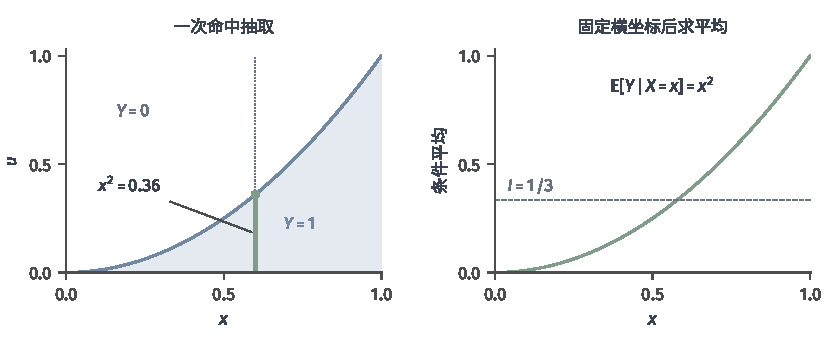
\includegraphics[width=140mm]{figures/00-shared/mathematical-preliminaries-lower/01-random-variables-distributions-and-causality/matplotlib/probability-rao-blackwell-slice/figure.pdf}
  \caption{命中积分的Rao--Blackwell化（解析式教学图）。独立的\(X,U\)均在\((0,1)\)上均匀分布。左图阴影为\(U\leq X^2\)，竖切片\(x=0.6\)的命中长度为\(0.36\)；右图保留每个\(x\)对应的条件均值\(x^2\)。两个变量的总体期望均为\(1/3\)，但方差分别为\(2/9\)与\(4/45\)。图中没有使用随机样本估计这些量。}
  \label{fig:probability-rao-blackwell-slice}
\end{figure*}

\subsection{未知归一化常数下的积分计算}
\paragraph{自归一化权重与比值估计}
重要性估计要求能计算正确归一化的概率比。但后验密度等目标常只知道相差一个公共常数的表达。把加权读数总和除以权重总和，可以消去这个未知常数；代价是分子、分母均随机，不能再沿用线性平均的有限样本无偏结论。
设\(P\ll Q\)，但只能在未知公共常数倍的意义下计算目标密度比，即对某个\(c>0\)，
\[
  \widetilde{w}(x)
  =
  c\,\frac{\mathrm{d}P}{\mathrm{d}Q}(x),
\]
在\(Q\)-几乎处处意义下成立。对独立同分布样本\(X_i\sim Q\)，在分母为正时使用
\(\widetilde{w}_i=\widetilde{w}(X_i)\)并定义
\begin{equation}
  \widehat{I}^{\mathrm{SN}}_n
  =
  \frac{\sum_{i=1}^{n}\widetilde{w}_if(X_i)}
       {\sum_{i=1}^{n}\widetilde{w}_i}.
  \label{eq:probability-self-normalized-importance-sampling}
\end{equation}
它是两个随机平均的比值，通常在有限样本下有偏，因为一般而言
\(\mathbb E[A/B]\ne\mathbb EA/\mathbb EB\)。一致性的证明及矩条件留到第~\ref{sec:rv-aggregate-limits}节。
若\(\widetilde w\)不是目标密度比的公共常数倍，归一化权重便描述另一个加权分布，不能据此声称估计的是\(\mathbb E_Pf\)。

\paragraph{权重截断、重采样与有效样本量}
一个三点分布可以同时看清方差、截断与重采样的不同作用。令支持集为
\(\{a,b,c\}\)，提议分布和目标分布分别为
\[
  Q=(0.8,0.15,0.05),\qquad
  P=(0.4,0.3,0.3),
\]
于是重要性权重为\(w=(0.5,2,6)\)。对
\(f=(0,1,1)\)，目标均值为\(I=0.6\)。原始单样本贡献
\(Z=wf=(0,2,6)\)满足
\[
  \mathbb{E}_Q Z=0.6,\qquad
  \operatorname{Var}_Q(Z)
  =\{0.15\times4+0.05\times36\}-0.6^2
  =2.04.
\]
因此\(n\)个独立样本的无偏估计方差为\(2.04/n\)。若把权重截断在\(2\)，则
\(w^{(2)}=(0.5,2,2)\)，相应贡献的期望变为\(0.4\)，方差变为
\[
  \{0.15\times4+0.05\times4\}-0.4^2=0.64.
\]
截断降低了方差，却引入\(-0.2\)的偏差；两者必须同时报告。

再看一组恰好含\(16\)个\(a\)、\(3\)个\(b\)和\(1\)个\(c\)的二十粒子样本。
原始权重总和为\(20\)，归一化后的三点质量恰为\((0.4,0.3,0.3)\)。按这些质量做
\(20\)次多项重采样，三点后代数的条件期望为\((8,6,6)\)；重采样后无权平均的条件
期望仍为\(0.6\)，但条件方差增加了
\[
  \frac{0.6(1-0.6)}{20}=0.012.
\]
若先截断，归一化质量变成\((0.5,0.375,0.125)\)，重采样均值的条件期望是\(0.5\)，
不会恢复被截断改变的目标。原始和截断权重在这组粒子上的经验有效样本量分别约为
\(400/52=7.69\)与\(256/20=12.8\)：较均匀的权重提高了这一诊断量，但不证明偏差消失。

经验有效样本量常写成
\[ \widehat{n}_{\mathrm{eff}}
  =\frac{(\sum_i\widetilde{w}_i)^2}{\sum_i\widetilde{w}_i^2}. \]
它是权重退化的诊断量，不是对所有估计目标都成立的精确独立样本数。截断权重可降低
方差，却通常引入偏差；重采样减少后续计算中的权重不均，却增加额外随机性。本节的“自归一化”是随机比值估计，第~\ref{sec:stoch-self-normalized-adaptive-design}节的自归一化集中则用随机设计矩阵度量累计噪声，二者对象不同。

\subsection{候选函数族的采样积分误差}
对每个候选函数\(f\in\mathcal F\)，都可用同一组独立样本计算\(n^{-1}\sum_i f(X_i)\)。当计算完成后还要根据样本选择\(f\)时，单个预先固定函数的误差界不足以覆盖这一选择。第~\ref{sec:probability-uniform-errors-symmetry}节的统一偏差界直接控制\(\sup_{f\in\mathcal F}|\widehat P_n f-Pf|\)，因而同时给出整族积分近似的保证。函数类的有界性、可测性及复杂度条件仍须逐项核对；重要性权重无界时，不能直接沿用有界函数类的结论。

\subsection{历史依赖观测的轨迹重加权}
\label{sec:stoch-trajectory-reweighting}
一次积分的变量也可以是整段随机轨迹。若记录来自一种逐步生成规则，而目标平均属于另一种规则，就需要对整段联合规律换测度；单个时刻的边缘比值不足以保留历史依赖。
对有限联合观测\(X_1,\ldots,X_n\)，若在同一逐步参考核下，两个规律的条件密度分别为
\(p_i(x_i\mid x_{<i})\)、\(q_i(x_i\mid x_{<i})\)，且初始及逐步目标核对来源核绝对连续，则
\[
\frac{\mathrm dQ}{\mathrm dP}(x_{1:n})
=\prod_{i=1}^n
\frac{q_i(x_i\mid x_{<i})}{p_i(x_i\mid x_{<i})}
\quad P\text{-几乎处处}.
\]
每个比值都要条件可测，并在实际可能到达的历史上归一化；对\(P\)不可能产生而\(Q\)可能产生的观测，不能用有限权重补救。此式只依赖联合分布的链式分解，不预设Markov性。下面在共同环境中比较两种行动策略，检查哪些条件因子能够相消。

% Baseline P:1257-1273
换测度也可作用于整段观测，而不只作用于一个随机变量。考虑长度\(T\)的轨迹
\(\tau=(s_0,a_0,s_1,a_1,\ldots,s_T)\)，其中\(s_t\)记录当前状态，\(a_t\)记录当步行动。
本段取离散状态与行动，核写成条件质量函数。假定行动只按当前状态的概率核\(\pi(a_t\mid s_t)\)产生，下一状态只按
\(P(s_{t+1}\mid s_t,a_t)\)产生，且这两个核不随时间改变。
初始分布为\(\rho\)时，条件概率的链式分解给出
\[ p_\pi(\tau)
  =\rho(s_0)\prod_{t=0}^{T-1}\pi(a_t\mid s_t)P(s_{t+1}\mid s_t,a_t). \]
若目标策略为\(\pi\)，采样策略为\(\mu\)，并且两者共享同一初始分布和环境转移核，公共因子相消，得到
\begin{equation}
  \frac{p_\pi(\tau)}{p_\mu(\tau)}
  =
  \prod_{t=0}^{T-1}
  \frac{\pi(a_t\mid s_t)}{\mu(a_t\mid s_t)}.
  \label{eq:probability-trajectory-likelihood-ratio}
\end{equation}
该公式要求目标轨迹分布绝对连续于采样轨迹分布。具体地说，只要\(\pi(a\mid s)>0\)，在可能到达的状态上就需要\(\mu(a\mid s)>0\)。共同环境假设若不成立，转移核的比值也必须保留。即使每一步
比值有限，长轨迹连乘仍可能产生极大方差；密度比存在并不提供可用的二阶误差界。

\section{随机序列与过程的收敛}
\label{sec:rv-sequence-process-convergence}
有限样本偏差界固定观测次数；本节让观测次数或演化时间增长，研究所产生序列的极限。平均值、标准化累计偏差、每步状态分布及整条路径分别属于不同空间。每种极限都要同时说明生成规则、比较方式与所求对象。

\subsection{随机误差的收敛关系}
\label{sec:probability-random-convergence-asymptotics}
“越来越接近”至少有三种不同含义：几乎每一条实现都收敛到目标，大偏差事件的概率趋于零，或者整体分布逐渐逼近某个极限分布。这三种收敛不能互换。本节先建立它们之间的蕴含关系，再讨论平均和缩放波动各自趋向什么。

\subsubsection{逐次偏差与样本路径的收敛}
\label{sec:rv-numerical-convergence}
% Baseline P:1310-1444
逐个时刻的尾概率还不足以判断一条样本路径是否反复进入坏事件。记
\[
  \limsup_{n\to\infty}A_n
  =
  \bigcap_{m=1}^{\infty}\bigcup_{n\geq m}A_n,
\]
它表示事件\(A_n\)发生无穷多次。
\begin{theorem}[Borel--Cantelli引理]
  \label{thm:probability-borel-cantelli}
  对事件序列\((A_n)_{n\geq1}\)，有以下两条结论。
  \begin{enumerate}
    \item 若\(\sum_{n=1}^{\infty}\mathbb{P}(A_n)<\infty\)，则
    \(\mathbb{P}(\limsup_n A_n)=0\)；这一方向不要求独立。
    \item 若事件\(A_1,A_2,\ldots\)相互独立，且其概率之和发散，即
    \[
      \sum_{n=1}^{\infty}\mathbb{P}(A_n)=\infty,
    \]
    则\(\mathbb{P}(\limsup_n A_n)=1\)。
  \end{enumerate}
\end{theorem}

\begin{proof}
对第一条，联合界给出
\[
  \mathbb{P}\left(\bigcup_{n\geq m}A_n\right)
  \leq\sum_{n\geq m}\mathbb{P}(A_n)\longrightarrow0.
\]
而\(\limsup_n A_n\)包含在每个尾并集中，故其概率为零。对第二条，固定\(m\)。独立性
给出
\[
  \mathbb{P}\left(\bigcap_{n=m}^{N}A_n^{\mathsf c}\right)
  =
  \prod_{n=m}^{N}\{1-\mathbb{P}(A_n)\}
  \leq
  \exp\left\{-\sum_{n=m}^{N}\mathbb{P}(A_n)\right\}
  \longrightarrow0.
\]
因此从任意\(m\)开始至少有一个\(A_n\)发生的概率都为一；再对可数个\(m\)取交，
便得到\(A_n\)几乎必然发生无穷多次。
\end{proof}

\par\medskip\noindent\textbf{随机收敛的四种方式}\quad
回用定义~\ref{def:probability-random-convergence}，现在证明各收敛方式之间的关系。Markov不等式给出
\[ \mathbb{P}(|X_n-X|>\varepsilon)
  \leq\frac{\mathbb{E}[|X_n-X|^p]}{\varepsilon^p}, \]
所以\(L^p\)收敛蕴含依概率收敛。

主要蕴含关系为
\[ X_n\to_{\mathrm{a.s.}}X
  \Longrightarrow X_n\to_{\mathbb{P}}X\Longrightarrow X_n\Rightarrow X, \]
以及\(L^p\)收敛蕴含依概率收敛。前两个蕴含可以直接证明。若
\(X_n\to_{\mathrm{a.s.}}X\)，则对固定\(\varepsilon>0\)，指示变量
\(\mathbb{I}\{|X_n-X|>\varepsilon\}\)几乎处处趋于\(0\)，并由常数\(1\)控制。支配收敛定理给出
\[
  \mathbb{P}(|X_n-X|>\varepsilon)
  =\mathbb{E}\mathbb{I}\{|X_n-X|>\varepsilon\}\to0.
\]
若\(X_n\to_{\mathbb{P}}X\)，对\(F_X\)的连续点\(x\)和任意\(\varepsilon>0\)，事件包含关系给出
\[
  F_X(x-\varepsilon)-\mathbb{P}(|X_n-X|>\varepsilon)
  \leq F_{X_n}(x)
  \leq
  F_X(x+\varepsilon)+\mathbb{P}(|X_n-X|>\varepsilon).
\]
先令\(n\to\infty\)，再令\(\varepsilon\downarrow0\)，由\(F_X\)在\(x\)处连续便得
\(F_{X_n}(x)\to F_X(x)\)。

反向一般不成立。令
\(U\sim\operatorname{Unif}(0,1)\)并取
\[ X_n=\sqrt{n}\mathbb{I}\{U\leq1/n\}. \]
则\(X_n\to0\)几乎必然且依概率成立，但\(\mathbb{E}[X_n^2]=1\)，所以不均方收敛。另一方面，可以安排概率为\(1/n\)的独立
事件\(A_n\)，令\(Y_n=\mathbb{I}_{A_n}\)。此时\(Y_n\to_{\mathbb{P}}0\)，但
\(\sum_n\mathbb{P}(A_n)=\infty\)，定理~\ref{thm:probability-borel-cantelli}的第二条
说明\(A_n\)几乎必然发生无穷多次，故\(Y_n\)不几乎必然收敛到零。

依分布收敛到常数时可以推出依概率收敛到该常数；依分布收敛到非退化随机变量则通常不能。若\(X\)关于原点对称，令\(X_n=-X\)，则\(X_n\)与\(X\)同分布，却不必有\(|X_n-X|\to0\)。

虽然依概率收敛不保证整列逐路径收敛，却允许从每条子列中找到逐路径收敛的进一步子列。这使我们可以先逐条实现使用确定性极限规则，再返回概率结论。
\begin{lemma}[依概率收敛的子列判据]
 \label{lem:rv-probability-subsequence}
 对同一概率空间中的度量空间值随机变量，\(X_n\to_{\mathbb P}X\)当且仅当每条子列都有进一步子列几乎必然收敛到\(X\)。
\end{lemma}
\begin{proof}
若依概率收敛，在任意子列中递归选取指标\(n_k\)，使
\[
  \mathbb P\{d(X_{n_k},X)>2^{-k}\}\leq2^{-k}.
\]
从第\(m\)项起的偏差事件并集概率至多为\(\sum_{k\geq m}2^{-k}\)，随\(m\to\infty\)趋于零。因此几乎必然只有有限个偏差事件发生，所选子列逐路径趋于\(X\)。
反之，若不依概率收敛，则存在\(\varepsilon,\eta>0\)及一条子列，其每项都满足
\(\mathbb P\{d(X_{n_k},X)>\varepsilon\}\geq\eta\)。
它不可能有几乎必然趋于\(X\)的进一步子列，否则对偏差指示函数使用支配收敛，概率将趋于零。
\end{proof}

\subsubsection{一致尾部控制下的平均误差收敛}
只控制大多数结果上的误差，还不能交换极限与期望：极少数结果可以贡献固定的平均质量。下面的条件直接限制这种尾部贡献。
\begin{definition}[一致可积]
  \label{def:probability-uniform-integrability}
可积随机变量族\(\{X_n\}\)若满足
\[
  \lim_{K\to\infty}
  \sup_n\mathbb{E}\bigl[
    |X_n|\mathbb{I}\{|X_n|>K\}
  \bigr]=0,
\]
就称为\term{一致可积}（uniformly integrable）。
\end{definition}
它排除了越来越小概率上的巨大取值仍承载固定期望质量。若
\(X_n\to_{\mathbb P}X\)且\(\{X_n\}\)一致可积，先由一致尾界得到
\(\sup_n\mathbb E|X_n|<\infty\)。选一个几乎必然收敛的子列，再用Fatou引理，便有\(X\in L^1\)。
令\(T_K(x)=\max\{-K,\min\{x,K\}\}\)，把误差拆成
\[
\begin{aligned}
\mathbb E|X_n-X|
 &\leq\mathbb E|X_n-T_K(X_n)|\\
 &\quad+\mathbb E|T_K(X_n)-T_K(X)|\\
 &\quad+\mathbb E|T_K(X)-X|.
\end{aligned}
\]
第一项由一致可积性随\(K\)增大而统一趋零，第三项由\(X\)可积趋零。
固定\(K\)后，从任意子列用引理~\ref{lem:rv-probability-subsequence}抽取几乎必然收敛的进一步子列；截断函数连续且中间差值不超过\(2K\)，故支配收敛使中项在该子列上趋零。若整列中项不趋零，就能选出始终大于某个正数的子列，与上述结论矛盾。
因此先令\(n\to\infty\)、再令\(K\to\infty\)，得到
\(\mathbb E|X_n-X|\to0\)。没有一致可积性，例如
\(V_n=n\mathbb{I}\{U\leq1/n\}\)虽几乎必然趋于\(0\)，却满足
\(\mathbb{E}V_n=1\)，小概率上的大幅值会阻止期望收敛。

图~\ref{fig:probability-vanishing-spikes}把这个反例画在同一个基础结果\(U\)上。尖峰变高时，其底宽按相同比例缩小；每条曲线下的面积仍是\(1\)。对任何固定\(K\)，只要\(n>K\)，全部面积都位于\(V_n>K\)的尾部，因此一致可积定义中的\(\sup_n\)不能趋于零。这里失败的是对整个变量族的统一尾部控制，而不是每条样本路径的收敛。
\begin{figure*}[htbp]
  \centering
  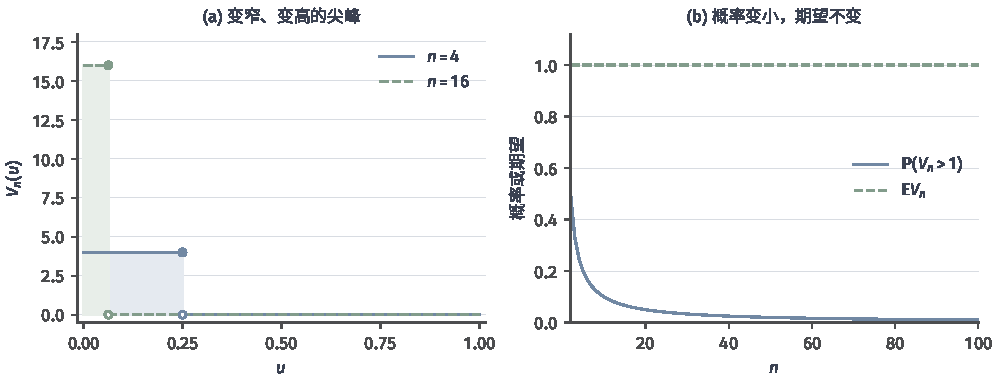
\includegraphics[width=\linewidth]{figures/00-shared/mathematical-preliminaries-lower/01-random-variables-distributions-and-causality/matplotlib/probability-vanishing-spikes/figure.pdf}
  \caption{小概率尖峰与期望质量（解析式教学图）。左图为\(V_n(u)=n\mathbb I\{u\leq1/n\}\)在\(n=4,16\)时的取值，均以面积\(1\)贡献期望；右图对\(n\geq2\)显示\(\mathbb P(V_n>1)=1/n\)趋于零，而\(\mathbb E V_n=1\)不变。基础变量为\(U\sim\operatorname{Unif}(0,1)\)。}
  \label{fig:probability-vanishing-spikes}
\end{figure*}
\subsubsection{历史条件均值约束下的序列收敛}
鞅关系约束每一步的条件均值，但是否存在长期极限仍需条件。非负超鞅的上穿论证给出一个基本结论。设$(L_t)$为非负超鞅且
$\mathbb{E}L_0<\infty$。对任意有理数$0<a<b$，记$U_n[a,b]$为
$L_0,\ldots,L_n$从不高于$a$到不低于$b$的完整上穿次数。在每次不高于$a$时持有一单位
过程、达到$b$时卖出；由于$(L_t)$是超鞅，这个可预测交易策略的期望收益不大于$0$。
比较每次完整交易至少$b-a$的路径收益与最后一次未完成交易，得到Doob上穿不等式
\[
  (b-a)U_n[a,b]
  \leq
  \text{交易收益}+(L_n-a)^-,
  \qquad x^-:=\max\{-x,0\}.
\]
其中负部$(L_n-a)^-$至多为$a$，而交易收益的期望不大于$0$。取期望得到
\[
  (b-a)\mathbb{E}U_n[a,b]
  \leq
  \mathbb{E}(L_n-a)^-
  \leq
  a.
\]
令$n\to\infty$可知每个正有理区间几乎必然只被上穿有限次。若$L_t$的下极限严格小于上
极限，就能在二者之间选到一个正有理区间并产生无穷多次上穿，形成矛盾。因此$L_t$几乎必然
存在扩展实数极限；再由Fatou引理与
$\sup_t\mathbb{E}L_t\leq\mathbb{E}L_0<\infty$排除极限为正无穷。于是非负超鞅几乎
必然收敛到有限随机变量。这个结论只保证路径极限存在；若还要交换极限与期望，仍需一致
可积等额外条件。
非负性不是鞅收敛的唯一入口。对有正有负的累计误差，常能控制的是二阶矩。
\begin{theorem}[二阶矩有界鞅的收敛]
\label{thm:rv-l2-martingale-convergence}
若\((M_n,\mathcal F_n)\)是平方可积鞅且
\(\sup_n\mathbb E M_n^2<\infty\)，则存在\(M_\infty\in L^2\)，使
\(M_n\to M_\infty\)几乎必然且在\(L^2\)中成立，并且
\(M_n=\mathbb E[M_\infty\mid\mathcal F_n]\)。
\end{theorem}
\begin{proof}
对\(m\geq n\)，条件均值性质给出
\(\mathbb E[M_n(M_m-M_n)]=0\)，所以
\[
\mathbb E(M_m-M_n)^2=\mathbb EM_m^2-\mathbb EM_n^2.
\]
右侧来自单调有界数列，故\(M_n\)在\(L^2\)中Cauchy，有\(L^2\)极限\(M_\infty\)。
还需将均方极限提升到整条序列的几乎必然极限。对有限鞅\(Y_j\)及
\(Y^*=\max_{j\leq N}|Y_j|\)，按首次越过水平\(a\)的时刻分解事件，并用
\(|Y_j|\leq\mathbb E[|Y_N|\mid\mathcal F_j]\)，得
\[
a\,\mathbb P(Y^*\geq a)
\leq\mathbb E[|Y_N|\mathbb I_{\{Y^*\geq a\}}].
\]
积分并用Cauchy--Schwarz，得到
\[
\begin{aligned}
 \mathbb E(Y^*)^2
 &\leq2\mathbb E(|Y_N|Y^*)\\
 &\leq2\|Y_N\|_2\|Y^*\|_2,
\end{aligned}
\]
故\(\mathbb E(Y^*)^2\leq4\mathbb E Y_N^2\)。
把它用于从\(n\)起的差鞅，再令有限终点趋于无穷，有
\[
\mathbb P\left\{\sup_{m\geq n}|M_m-M_n|>\varepsilon\right\}
\leq\frac4{\varepsilon^2}
\bigl(\mathbb EM_\infty^2-\mathbb EM_n^2\bigr).
\]
取子列\(n_k\)，使括号小于\(2^{-4k}\)，并取\(\varepsilon=2^{-k}\)，坏事件概率可求和。Borel--Cantelli表明整列几乎必然Cauchy，极限与\(L^2\)极限一致。
最后对\(A\in\mathcal F_n\)，令\(m\to\infty\)于
\(\mathbb E[M_m\mathbb I_A]=\mathbb E[M_n\mathbb I_A]\)，得到所述条件期望表示。
\end{proof}
随机逼近将用平方可和步长控制累计鞅噪声；状态本身是否收敛，还要结合稳定性与漂移，不能只用这一定理替代。

\subsection{重复采样下的平均序列收敛}

每增加一个独立读数，都把累计和除以新的样本数，得到\(\overline X_n=n^{-1}\sum_{i=1}^nX_i\)。所求极限是单次读数的总体均值。前面的有限预算界可以支持部分依概率结论；要使几乎每条无限实现都收敛，还需核对相应的大数定律条件。
\label{sec:rv-aggregate-limits}
% Baseline P:1448-1511
\begin{theorem}[强大数定律]
\label{thm:probability-strong-law-large-numbers}
若\(X_1,X_2,\ldots\)独立同分布，且\(\mathbb{E}[|X_1|]<\infty\)，则
\[ \overline{X}_n
  =\frac{1}{n}\sum_{i=1}^{n}X_i\to_{\mathrm{a.s.}}\mathbb{E}[X_1]. \]
\end{theorem}

强大数定律说明同一分布下的独立重复观测，其平均几乎必然接近期望。有限方差是许多初等证明使用的方便条件，但独立同分布版本的结论只需有限一阶绝对矩。若观测相关、分布随
时间变化或样本由自适应规则收集，则不能直接引用该定理；第~\ref{sec:stoch-markov-long-run-average}节给出相关过程的一组替代条件\scite{math-kallenberg2021probability}。

有限方差时，较弱的依概率结论可以在这里完整得到。若
\(\operatorname{Var}(X_1)=\sigma^2<\infty\)，独立性使
\[
  \operatorname{Var}(\overline{X}_n)
  =\frac{1}{n^2}\sum_{i=1}^{n}\operatorname{Var}(X_i)
  =\frac{\sigma^2}{n}.
\]
把\BookEquationRef{eq:probability-chebyshev-inequality}{式~\eqref{eq:probability-chebyshev-inequality}}用于样本平均，有
\[
  \mathbb{P}\bigl(
    |\overline{X}_n-\mathbb{E}X_1|\geq\varepsilon
  \bigr)
  \leq\frac{\sigma^2}{n\varepsilon^2}\to0.
\]
这证明了有限方差版本的弱大数定律。强大数定律只要求有限一阶绝对矩，但其证明还需截断大取值、控制截断变量的独立和，并把可求和坏事件转成几乎必然结论；不能由上面的逐个\(n\)概率界直接推出。

对例~\BookReference{ex:probability-noisy-observation}{\ref{ex:probability-noisy-observation}}中的独立同分布噪声，只要\(\mathbb{E}|\varepsilon_i|<\infty\)，便有
\[ \overline{Y}_n
  =\theta+\frac{1}{n}\sum_{i=1}^{n}\varepsilon_i\to_{\mathrm{a.s.}}\theta. \]
这回答了“多测几次再平均是否稳定”，但没有给出固定\(n\)时误差超过指定阈值的概率。

\subsection{重复采样下的标准化累计偏差序列分布收敛}

平均值接近总体均值后，仍可考察剩下的随机波动。先从累计和中减去\(n\mu\)，再除以独立累计的标准差\(\sigma\sqrt n\)，得到\((\sum_{i=1}^nX_i-n\mu)/(\sigma\sqrt n)\)。这个序列通常不趋于一个固定数；在下面的条件下，它的分布趋于标准高斯。
\label{sec:rv-standardized-sum-limits}
\begin{theorem}[Lindeberg--L\'evy中心极限定理]
\label{thm:probability-iid-central-limit}
若\(X_1,X_2,\ldots\)独立同分布，\(\mathbb{E}X_1=\mu\)，\(0<\operatorname{Var}(X_1)=\sigma^2<\infty\)，则
\[ \frac{\sqrt{n}(\overline{X}_n-\mu)}{\sigma}
  \Rightarrow\mathcal{N}(0,1). \]
\end{theorem}

大数定律研究未缩放误差是否趋于零，中心极限定理研究乘以\(\sqrt{n}\)后的剩余波动近似什么分布。它给出渐近近似，而不是每个有限\(n\)都精确服从高斯分布。若方差
无限、样本依赖过强或分布随\(n\)变化而不满足相应Lindeberg条件，\(\sqrt{n}\)缩放与高斯极限都可能失效。

证明的关键是特征函数。令\(Y_i=(X_i-\mu)/\sigma\)，并记
\(\varphi(t)=\mathbb{E}e^{\mathrm{i}tY_1}\)。复指数绝对值恒为\(1\)，所以特征函数总有定义。由
\(\mathbb{E}Y_1=0\)、\(\mathbb{E}Y_1^2=1\)及零点处的二阶展开，
\[
  \varphi(u)=1-\frac{u^2}{2}+o(u^2),
  \qquad u\to0.
\]
独立性使标准化和的特征函数分解为
\[
  \mathbb{E}\exp\left\{
    \mathrm{i}t\frac{1}{\sqrt n}\sum_{i=1}^{n}Y_i
  \right\}
  =
  \left[\varphi\left(\frac{t}{\sqrt n}\right)\right]^n
  \longrightarrow e^{-t^2/2}.
\]
右侧是标准高斯的特征函数，并且在零点连续。\BookTheoremRef{thm:probability-levy-continuity}{定理
~\ref{thm:probability-levy-continuity}}于是给出依分布收敛。\BookSectionRef{sec:statistics-intervals-quantiles}{第
~\ref{sec:statistics-intervals-quantiles}节}使用这个渐近分布构造近似区间，但有限样本覆盖
仍需额外误差控制，不能只引用极限式。
\subsection{随机误差变换后的极限}
\label{sec:stoch-random-transform-limits}
样本平均的极限并不是所有计算的最终输出：归一化会引入随机分母，非线性变换还会改变误差尺度。先检查随机余项的大小，再传递连续变换和常数极限，才能判断新输出的长期波动。

\subsubsection{概率阶运算与随机误差的组合}
为控制非线性变换中的乘积余项，再核对两条概率阶规则。若\(Z_n\xrightarrow{\mathrm d}Z\)，对任意
\(\epsilon>0\)，可取充分大的\(M\)使
\(\mathbb{P}(|Z|\geq M)<\epsilon/2\)。依分布收敛的闭集上界给出
\[
  \limsup_{n\to\infty}\mathbb{P}(|Z_n|\geq M)
  \leq \mathbb{P}(|Z|\geq M)<\epsilon/2,
\]
所以\(Z_n=O_{\mathbb{P}}(1)\)。此外，若
\(A_n=o_{\mathbb{P}}(1)\)、\(B_n=O_{\mathbb{P}}(1)\)，则对任意
\(\eta,\epsilon>0\)，先取\(M\)使大样本下
\(\mathbb{P}(|B_n|>M)<\epsilon/2\)，再取充分大的\(n\)使
\(\mathbb{P}(|A_n|>\eta/M)<\epsilon/2\)。于是
\[
  \mathbb{P}(|A_nB_n|>\eta)
  \leq
  \mathbb{P}(|B_n|>M)
  +\mathbb{P}(|A_n|>\eta/M)
  <\epsilon,
\]
即\(o_{\mathbb{P}}(1)O_{\mathbb{P}}(1)=o_{\mathbb{P}}(1)\)。


\subsubsection{连续变换与随机因子的极限传递}
若样本平均趋近一个非零常数，取倒数是否仍趋近该常数的倒数，取决于极限处的连续性。一般连续变换先沿逐条实现传递极限；依概率和依分布的结论再分别使用子列判据与闭集概率控制。
\begin{theorem}[连续映射]
\label{thm:rv-continuous-mapping}
若\(X_n\to X\)几乎必然或依概率，且可测函数\(g\)在\(X\)的取值处几乎必然连续，则\(g(X_n)\to g(X)\)具有相应收敛方式。
若\(X_n\Rightarrow X\)且\(\mathbb P(X\in D_g)=0\)，其中\(D_g\)为\(g\)的不连续点集，则\(g(X_n)\Rightarrow g(X)\)。变量可取值于Polish空间。
\end{theorem}
\begin{proof}
几乎必然情形逐条在连续点应用确定序列的极限规则。依概率情形使用子列判据：每个子列都有一个几乎必然收敛的子子列，应用前一结论，再用同一判据返回依概率收敛。依分布情形对闭集\(C\)，有
\(\overline{g^{-1}(C)}\subseteq g^{-1}(C)\cup D_g\)；\BookTheoremRef{thm:rv-portmanteau}{定理~\ref{thm:rv-portmanteau}}的闭集上界给出
\(\limsup_n\mathbb P(g(X_n)\in C)\leq\mathbb P(g(X)\in C)\)，即得结论。
\end{proof}
例如倒数映射在零不连续；只有极限以概率一非零时才可直接取倒数。均方收敛不能对任意连续函数自动传递，因为变换可能放大尾部。
% Baseline T:562-634
\begin{theorem}[Slutsky定理]
  \label{thm:statistics-slutsky}
  若\(X_n\xrightarrow{\mathrm d}X\)，且
  \(Y_n\xrightarrow{\mathbb{P}}c\)，其中\(c\)为常数，则
  \[
    X_n+Y_n\xrightarrow{\mathrm d}X+c,\qquad
    X_nY_n\xrightarrow{\mathrm d}cX.
  \]
  若\(c\neq0\)，还有
  \(X_n/Y_n\xrightarrow{\mathrm d}X/c\)。比值在\(Y_n=0\)的事件上可补为任意固定值；这些事件的概率趋于零，因而不影响该分布极限。特别地，若
  \(R_n=o_{\mathbb{P}}(1)\)，则
  \(X_n+R_n\xrightarrow{\mathrm d}X\)。
\end{theorem}

\begin{proof}
先证明和的结论。任取\(\varepsilon>0\)，记\(p_n=\mathbb P(|Y_n-c|>\varepsilon)\)。事件包含关系给出
\[
 F_{X_n}(x-c-\varepsilon)-p_n
 \leq F_{X_n+Y_n}(x)
 \leq F_{X_n}(x-c+\varepsilon)+p_n.
\]
在\(F_{X+c}\)的连续点\(x\)，先令\(n\to\infty\)，再沿使两端均为\(F_X\)连续点的\(\varepsilon\downarrow0\)，得到\(F_{X_n+Y_n}(x)\to F_{X+c}(x)\)。

依分布收敛使\(X_n=O_{\mathbb P}(1)\)，而\(Y_n-c=o_{\mathbb P}(1)\)，故前面的概率阶规则给出\(X_n(Y_n-c)=o_{\mathbb P}(1)\)。将
\(X_nY_n=cX_n+X_n(Y_n-c)\)代入刚证明的和的结论，并对\(cX_n\)应用连续映射，即得乘积结论，包括\(c=0\)的退化情形。若\(c\neq0\)，连续映射还使\(1/Y_n\to_{\mathbb P}1/c\)，再用乘积结论得到比值。零分母事件包含在\(\{|Y_n-c|\geq|c|\}\)中，概率趋于零，因此该事件上的约定不影响极限。
\end{proof}

Slutsky定理允许把收敛到常数的标准误、归一化因子或余项代入渐近分布。它不表示两个一般
随机极限可以忽略联合分布；关键条件是其中一个序列依概率收敛到常数。

均值的标准误估计若依概率趋向正确的正尺度，Slutsky定理就允许在渐近统计量中代入它。条件是标准误的随机极限正确，不能由一次算出的数值看起来合理来代替。非线性函数的缩放误差将在定理~\ref{thm:statistics-delta-method}中进一步用Taylor展开处理。
% Baseline T:636-743
现在可以回到第~\ref{sec:probability-monte-carlo-variance-reduction}节，逐项核验积分近似的长期条件。直接平均只要
\(\mathbb E|f(X)|<\infty\)就强一致，若再有有限正方差，则中心极限定理给出
\(\sqrt n(\widehat I_n-I)\Rightarrow\mathcal N(0,\operatorname{Var}(f(X)))\)。
重要性采样把\(f(X)\)换成\(w(X)f(X)\)，因此要在来源分布下分别查
\(\mathbb E|wf|\)和\(\mathbb E[(wf)^2]\)；密度比存在并不推出第二项有限。

控制变量使用预先固定的系数及已知均值时，同样对修正后的被积量检查一阶、二阶矩。若系数由同一数据估计，无偏性可能不再成立；在系数一致、控制变量有适当矩等条件下，可用Slutsky分析其余项，不能直接照搬固定系数公式。Rao--Blackwell化的条件期望保留一阶可积性，在二阶可积时又由条件Jensen不等式不增方差。

自归一化重要性估计是两个平均的比。设非归一化权重\(\widetilde w\geq0\)，
\(0<Z=\mathbb E_Q\widetilde w<\infty\)，且
\(\mathbb E_Q|\widetilde wf|<\infty\)。沿用\(\widetilde w/Z=\mathrm dP/\mathrm dQ\)
及独立同分布的\(Q\)样本，两个强大数定律和连续映射给出
\[
\frac{\sum_i\widetilde w(X_i)f(X_i)}
{\sum_i\widetilde w(X_i)}
\longrightarrow
\frac{\mathbb E_Q[\widetilde wf]}Z=I
\quad\text{几乎必然}.
\]
分母由强大数定律最终远离零。若
\(\mathbb E_Q[\widetilde w^2(1+f^2)]<\infty\)，可把中心化比值直接写成
\[
 \sqrt n(\widehat I_{\mathrm{SN}}-I)
 =\frac{n^{-1/2}\sum_{i=1}^n
       \widetilde w(X_i)(f(X_i)-I)}
       {n^{-1}\sum_{i=1}^n\widetilde w(X_i)}.
\]
分子的求和项独立同分布，均值为零，方差为
\(\mathbb E_Q[\widetilde w^2(f-I)^2]\)。方差为正时，标量中心极限定理给出分子的高斯极限；分母强收敛到\(Z>0\)，再用Slutsky定理，得到渐近方差
\[
\frac{\mathbb E_Q[\widetilde w^2(f-I)^2]}{Z^2}.
\]
若该方差为零，分子各项几乎必然为零，极限相应退化为零常量。
这没有消除有限样本比值偏差。固定阈值截断权重通常收敛到截断后的目标；若希望阈值随样本量增长而仍恢复原积分，还要证明被截去尾部和随机误差同时消失。

\subsubsection{非线性变换后的渐近波动}
连续映射保证变换后的结果趋近目标，但没有说明误差乘以何种尺度后仍有非退化极限。若原误差具有高斯极限，局部线性近似会把变换的导数带入渐近方差。

\begin{theorem}[Delta方法]
\label{thm:statistics-delta-method}
若
\(\sqrt n(\widehat\theta_n-\theta)\xrightarrow{\mathrm d}\mathcal N(0,V)\)，
且\(g\)在\(\theta\)处可微，则
\[
  \sqrt n\bigl(g(\widehat\theta_n)-g(\theta)\bigr)
  \xrightarrow{\mathrm d}
  \mathcal N\bigl(0,g'(\theta)^2V\bigr).
\]
\end{theorem}

\begin{proof}
记
\[
  Z_n=\sqrt n(\widehat\theta_n-\theta),
  \qquad
  Z\sim\mathcal N(0,V).
\]
前面已证明依分布收敛推出概率有界，以及\(o_{\mathbb P}(1)O_{\mathbb P}(1)=o_{\mathbb P}(1)\)，故\(Z_n=O_{\mathbb P}(1)\)。

特别地，
\(\widehat\theta_n-\theta=n^{-1/2}Z_n=o_{\mathbb{P}}(1)\)，所以估计量依概率一致。
Taylor展开给出
\[
  g(\widehat\theta_n)-g(\theta)
  =g'(\theta)(\widehat\theta_n-\theta)
   +r_n(\widehat\theta_n-\theta),
\]
其中一致性与可微性保证\(r_n=o_{\mathbb{P}}(1)\)。乘以\(\sqrt n\)后，
余项是
\(r_nZ_n=o_{\mathbb{P}}(1)\)。主项由假设依分布收敛，再用Slutsky定理即得结论。
\end{proof}

例如若某估计量满足
\(\sqrt n(\widehat\theta_n-\theta)\Rightarrow\mathcal N(0,\sigma^2)\)，且
\(\theta>0\)，取\(g(\theta)=\log\theta\)，其渐近方差为
\(\sigma^2/\theta^2\)。估计量以趋于一的概率落在正半轴；在非正事件上任取一个约定值不影响极限。
若\(g'(\theta)=0\)，一阶Delta方法仍成立，但只给出零方差的退化极限；要描述非退化波动，需要更高阶展开与新的缩放。若\(g\)在目标点不可微，才不能直接应用上述定理。

\paragraph{方差稳定化与逆变换偏差}
不同均值的计数往往具有不同的方差。若希望在统一的误差尺度上处理这些读数，需要选取一种非线性变换，使变换后的渐近方差尽量不依赖未知均值。设独立同分布观测的均值为\(\mu\)，方差为已知函数形式\(V(\mu)>0\)，并且样本平均满足
\[
 \sqrt n(\overline X_n-\mu)\Rightarrow\mathcal N(0,V(\mu)).
\]
Delta方法使\(g(\overline X_n)\)的渐近方差变为\(g'(\mu)^2V(\mu)\)。因此在\(V\)正且连续的区间上，取
\begin{equation}
 g(x)=\int^x\frac{1}{\sqrt{V(u)}}\,\mathrm du,
 \qquad
 \sqrt n\{g(\overline X_n)-g(\mu)\}
 \Rightarrow\mathcal N(0,1),
 \label{eq:stoch-variance-stabilizing-delta}
\end{equation}
就得到\term{方差稳定化变换}（variance-stabilizing transform）。积分下限只改变常数偏移，不改变导数和误差方差；均值须处在所用区间内部，以保证局部展开有效。这是关于渐近波动的结论，不宣称有限样本方差精确相同。

Poisson观测满足\(V(\mu)=\mu\)。在\(\mu>0\)处，上式给出\(g(x)=2\sqrt x\)；若\(\mu=0\)，观测恒为零，不能沿用这里的非退化高斯极限。对单次均值很大的计数\(Y\sim\operatorname{Poisson}(\lambda)\)，局部Taylor近似同样给出
\(\operatorname{Var}(g(Y))\approx g'(\lambda)^2\lambda=1\)。进一步的高阶修正得到常用Anscombe变换
\[
 A(Y)=2\sqrt{Y+3/8}.
\]
其中\(3/8\)不是一阶Delta方法本身推出的常数，而是改善方差近似的修正；低计数时仍不能把离散变换结果视为精确的单位方差高斯读数\scite{vision-anscombe1948}。

对\BookSectionRef{sec:rv-combinations}{第~\ref{sec:rv-combinations}节}的信号相关噪声模型，令\(Y=\alpha K+\varepsilon\)，其中\(\alpha>0\)、\(\mu\geq0\)、\(K\sim\operatorname{Poisson}(\mu/\alpha)\)，\(\varepsilon\sim\mathcal N(0,\sigma^2)\)，并假定二者独立，则
\(\mathbb EY=\mu\)、\(\operatorname{Var}(Y)=\alpha\mu+\sigma^2\)。同一导数条件给出
\[
 g(y)=\frac2\alpha\sqrt{\alpha y+\sigma^2}.
\]
这说明平方根形式如何承接线性变化的方差。该局部近似要求均值处于根号内为正且相对波动足够小的区域；高斯噪声可能使实际读数落到\(\alpha y+\sigma^2<0\)处。若对这类读数截断后再变换，就已改变变换规则及其误差，需另行核验，不能把上式当作全实轴上的精确稳定化。

逆变换也必须区分输入对象。未经处理的读数满足\(A^{-1}(A(Y))=Y\)，代数逆并不改变原读数的均值。但若在变换域平滑后，输出接近的是\(m(\lambda)=\mathbb E_\lambda A(Y)\)，则恢复\(\lambda\)需要反演函数\(m\)，不是直接对这个均值应用\(A^{-1}\)。这里甚至可以精确计算两者的差别：由于\(A(Y)^2=4Y+3/2\)，
\begin{equation}
 A^{-1}(m(\lambda))
 =\frac{m(\lambda)^2}{4}-\frac38
 =\lambda-\frac14\operatorname{Var}_\lambda(A(Y)).
 \label{eq:stoch-anscombe-inverse-bias}
\end{equation}
当\(\lambda>0\)时，右端严格小于\(\lambda\)。若变换后方差约为一，偏差便约为\(-1/4\)；变换域的平均估计即使准确，代数逆仍会引入这一系统偏移。按\(m(\lambda)\mapsto\lambda\)建立的校正逆能够消除此处由均值映射造成的偏差，但对带有额外估计误差的任意平滑输出，并不自动保证总体无偏。低计数下的逆变换校正和具体去噪计算可参考原始研究，应用模型留给图像处理部分\scite{vision-makitalo2011anscombe}。

\subsection{状态转移下的时间平均序列收敛}
\label{sec:stoch-markov-long-run-average}

沿同一条Markov轨迹计算\(n^{-1}\sum_{t=1}^n f(Z_t)\)，每次新读数都与此前状态相关。我们现在要判断这条时间平均序列是否识别平稳分布下的\(\mathbb E_\pi f\)。对有限不可约链，可以把返回某个状态的路径切成独立游程，再回用重复采样的强大数定律。
更具体地，状态\(i\)到\(j\)可达，是指存在\(m\geq0\)使\(P^m(i,\{j\})>0\)。
令\(T_i^+=\inf\{t\geq1:Z_t=i\}\)；若
% Baseline S:199-358
$\mathbb{P}_i(T_i^+<\infty)=1$，就称$i$为\term{常返状态}（recurrent state）。
有限多个互达类之间不可能沿可达关系循环而仍属于不同的类，因此沿可达关系前进，总能到达一个封闭类。
在有限不可约链中，还能得到比概率一返回更强的界：固定$i$，从每个状态选一条正概率、正长度的路径到$i$。
由于状态数有限，存在统一的整数$M$与$\varepsilon>0$，使从任意状态在接下来$M$步内访问$i$的概率至少为$\varepsilon$。
按长度$M$的时间块使用Markov性质，得到
\[
 \mathbb P_i(T_i^+>kM)\leq(1-\varepsilon)^k,\qquad
 \mathbb E_iT_i^+\leq M/\varepsilon<\infty.
\]
所以所有状态常返，且平均返回时间有限。对一般有限链的每个封闭类，在类内应用相同论证，也说明它是常返类。

从$i$出发，把从一次访问$i$起、到下一次返回$i$前为止的路径作为一个游程。返回时刻只由已经观察到的历史决定，属于定义~\ref{def:stoch-stopping-time}中的停时。Markov性质在这类随机时刻之后仍成立，称为强Markov性；在有限离散链中，把返回时刻的各个可能取值分别代入Markov条件即可验证。因此这些游程独立同分布。记第$k$个游程的长度为$L_k$、其中访问$j$的次数为
$R_k$。已证$\mathbb E_iL_1<\infty$，又有$0\leq R_k\leq L_k$，故可对两组变量使用强大数定律：
\[
  \frac{\sum_{k=1}^{m}R_k}{\sum_{k=1}^{m}L_k}
  \longrightarrow
  \frac{\mathbb{E}_iR_1}{\mathbb{E}_iL_1}
  \quad\text{几乎必然成立。}
\]
长期时间占比来自多个游程的累计比值，而不是单次随机比值$R_k/L_k$。
为识别右侧极限，先确认有限不可约链的平稳概率存在且唯一。任取初始概率向量\(\bm\nu\)，Ces\`aro平均\(n^{-1}\sum_{t=0}^{n-1}\bm\nu^{\top}\bm P^t\)都在有限维概率单纯形中，故有收敛子列。该平均乘\(\bm P\)前后的差为\((\bm\nu^{\top}\bm P^n-\bm\nu^{\top})/n\to\bm0\)，因此子列极限平稳。不可约性又使任意非零非负平稳向量的每个坐标都为正：若某坐标为零，所有能在若干步到达它的正坐标都会使平稳等式矛盾。若有两个平稳概率\(\bm\pi,\bm\rho\)，取\(c=\min_j\pi_j/\rho_j>0\)，则\(\bm\pi-c\bm\rho\)平稳、非负且至少一坐标为零，只能是零向量；再由归一化得到\(c=1\)及\(\bm\pi=\bm\rho\)。

现在记
$a_j=\mathbb E_i\sum_{t=0}^{L_1-1}\mathbb I\{Z_t=j\}$。
对每个$t$，事件$\{t<L_1\}$属于$\mathcal F_t$；逐项条件化并使用非负换序，得
\[
\begin{aligned}
 \sum_\ell a_\ell\bm P_{\ell,j}
 &=\mathbb E_i\sum_{t=0}^{L_1-1}\bm P_{Z_t,j}\\
 &=\mathbb E_i\sum_{t=0}^{L_1-1}\mathbb I\{Z_{t+1}=j\}
 =a_j.
\end{aligned}
\]
最后一步把计数区间从$0,\ldots,L_1-1$移到$1,\ldots,L_1$；因游程首尾都为$i$，总计数不变。
又有$\sum_j a_j=\mathbb E_iL_1$，所以归一化向量
$a_j/\mathbb E_iL_1$满足平稳方程，由唯一性就是$\pi_j$。
取$j=i$时每个游程恰计一次访问，因而$\pi_i=1/\mathbb E_iT_i^+$。

以上比值只覆盖完整游程，还须控制任意时刻剩下的一段。
令$A_m=\sum_{k=1}^mL_k$，强大数定律给出$A_m/m\to\mathbb E_iL_1$，相减即得
$L_m/m=A_m/m-A_{m-1}/m\to0$。
对$A_m\leq n<A_{m+1}$，未完成游程至多贡献$L_{m+1}$次访问，而
$L_{m+1}/A_m\to0$，因此它不改变时间占比的极限。
从任意其他初态出发，到首次访问$i$的时间也由上述几何尾界控制；
这段有限初始路径除以$n$后趋零。由此才得到对每个整数$n$及任意初态成立的遍历平均。

不可约性与非周期性在这里服务于逐时刻分布收敛。时间平均的要求略有不同：有限不可约链
即使有周期，对每个函数
$f:\mathcal{Z}\to\mathbb{R}$仍有
\begin{equation}
  \frac1n\sum_{t=1}^{n}f(Z_t)\longrightarrow\mathbb{E}_{\pi}[f(Z)]
  \quad\text{几乎必然成立。}
  \label{eq:stoch-markov-ergodic-average}
\end{equation}
例如在$0$与$2$之间确定性交替的链具有周期$2$。从$0$出发时，$Z_t$的分布在两个点之间
来回切换，不存在逐步极限；但时间平均仍趋向$1$。因此，讨论“遍历”时必须说明结论针对
逐步分布、时间平均还是其他对象。

例~\ref{ex:stoch-two-state-chain}没有这些退化。其第二个特征值为$0.7$。令
$\widetilde{Y}_t=Y_t-\mu$，直接计算可得
\begin{equation}
  \mathbb{E}[\widetilde{Y}_{t+1}\mid Z_t]=0.7\widetilde{Y}_t.
  \label{eq:stoch-two-state-eigenfunction}
\end{equation}
反复使用塔式性质便得到
$\mathbb{E}[\widetilde{Y}_{t+k}\mid Z_t]=0.7^k\widetilde{Y}_t$。
若链从平稳分布启动，
\begin{equation}
  \operatorname{Corr}_{\pi}(Y_t,Y_{t+k})=0.7^k.
  \label{eq:stoch-two-state-autocorrelation}
\end{equation}
这个几何衰减同时展示了“收敛到平稳”和“样本之间仍相关”：边缘分布可以从一开始就等于
$\pi$，相邻观测却不会因此独立。

\par\medskip\noindent\textbf{一般状态空间的返回条件}\quad
有限链可用矩阵、路径和周期描述可达性。连续或一般状态空间中，单点通常概率为零，“每个
状态互相到达”不再是合适表述。
\begin{definition}[一般状态空间的不可约性与Harris常返性]
  \label{def:stoch-harris-recurrence}
固定$(\mathcal{Z},\mathcal{A})$上的非零参考测度
$\varphi$。常用的$\varphi$不可约性要求：对每个满足$\varphi(B)>0$的
$B\in\mathcal{A}$以及每个初态$z\in\mathcal{Z}$，链从$z$出发都有正概率在有限时间内
到达$B$；若只研究某个不可约类，就先把$\mathcal{Z}$限制为该类。在此基础上，
\term{Harris常返性}（Harris recurrence）要求这些正测度集合以概率$1$被反复访问；
\term{正Harris常返性}（positive Harris recurrence）再要求存在不变概率分布。这里的反复访问要求：对每个上述\(B\)和每个初态\(z\)，以概率\(1\)有无穷多个\(t\geq0\)满足\(Z_t\in B\)。
\end{definition}
对
$\pi$可积的$f$，正Harris常返性提供一般状态空间遍历大数定律的标准入口。

这里“反复访问”带有概率$1$的量词：从$\mathcal{Z}$中的任意初态出发，每个满足
$\varphi(B)>0$的集合$B$都几乎必然被访问无穷多次。仅有“以正概率最终到达”还不够，
因为过程仍可能以正概率逃离后永不返回。正Harris常返链对其唯一不变概率$\pi$满足
式~\eqref{eq:stoch-markov-ergodic-average}的一般状态空间版本，但函数必须
$\pi$可积；若只知道局部可积或某个初态下样本值有限，不能推出该时间平均结论。

这些条件也解释了相关平均的边界。链若可约，长期平均可能由初始封闭类决定；链若只保持
$\pi$而不能充分移动，有限预算误差可能很大；观测函数若不可积，平稳分布存在也不能定义
所求均值。第~\ref{chap:dynamical-systems-and-state-estimation}章会把相关观测用于均值求根
式~\eqref{eq:stoch-mean-root}；这里提供的前提是长期平均确实识别目标均值，
而不是把相关的$Y_t$假装成独立样本。

\par\medskip\noindent\textbf{相关平均的有限样本方差}\quad
时间平均的极限确定了估计目标；有限观测下的精度还取决于跨时刻相关。下面在平稳初态下直接展开平均值的方差。
若链平稳，且观测函数具有有限正方差，记
\[
\sigma_f^2=\operatorname{Var}_{\pi}(f(Z_0)),\qquad 0<\sigma_f^2<\infty.
\]
它在间隔\(k\)处的自相关为
\[
\rho_f(k)=\operatorname{Corr}_{\pi}(f(Z_0),f(Z_k)).
\]
展开样本均值方差得到
\begin{align}
  \operatorname{Var}\left(
    \frac1n\sum_{t=1}^{n}f(Z_t)
  \right)
  &=
  \frac{\sigma_f^2}{n}
  \left[
    1+
    2\sum_{k=1}^{n-1}
      \left(1-\frac{k}{n}\right)\rho_f(k)
  \right].
  \label{eq:stoch-markov-average-variance}
\end{align}
若$\sum_{k\geq1}|\rho_f(k)|<\infty$，括号中的量趋向
\[
  \tau_f
  =
  1+2\sum_{k=1}^{\infty}\rho_f(k),
\]
称为积分自相关时间。它是非负的渐近方差比；在\(\tau_f>0\)时，用$n_{\mathrm{eff}}\approx n/\tau_f$表达
\term{自相关有效样本量}（autocorrelation effective sample size），只是把该函数
均值的渐近方差换算成独立样本尺度。它依赖$f$，也不同于重要性权重的有效样本量。若\(\sigma_f^2=0\)，观测函数在平稳分布下为常数，无须定义相关系数；若\(\tau_f=0\)，则\(n\operatorname{Var}(\overline f_n)\to0\)，不能用有限的\(n/\tau_f\)概括其误差。

对例~\ref{ex:stoch-two-state-chain}，式
\eqref{eq:stoch-two-state-autocorrelation}给出
\[
  \tau_Y=1+2\sum_{k=1}^{\infty}0.7^k
  =\frac{1+0.7}{1-0.7}=\frac{17}{3}.
\]
因而长链对均值$\mu$提供的信息量约为$3n/17$个独立观测，而不是$n$个。若自相关为负，
$\tau_f$也可能小于$1$；有效样本量是特定估计量的方差等价口径，不是链中“真正保留下来”
的样本条数。

\subsection{状态转移下的分布序列收敛}
\label{sec:rv-state-distribution-limits}
上一节的时间平均可以在逐时刻分布振荡时仍然收敛。现在固定初始状态，比较每步状态的分布\(P^t(z,\cdot)\)是否趋于\(\pi\)。在有限不可约链中，
$\bm{P}^{\top}$的特征值$1$对应唯一的概率右特征向量$\bm{\pi}$；等价地，
$\bm{\pi}^{\top}$是行随机转移矩阵$\bm{P}$的唯一概率左特征向量。加入非周期性后，
其他模态不会在单位圆上持续振荡，矩阵幂$\bm{P}^t$才逐行趋于
$\bm{\pi}^{\top}$。这两条路线分别解释了为什么周期不妨碍时间占比，却会妨碍逐时刻分布
收敛。

有限、不可约、非周期链满足
\begin{equation}
  P^t(z,\cdot)\longrightarrow\pi(\cdot)
  \quad\text{对每个初始状态 }z,
  \label{eq:stoch-finite-chain-distribution-convergence}
\end{equation}
其中有限状态下的收敛可以用\term{总变差距离}（total variation distance）衡量。这一距离比较所有事件概率，\BookDefinitionRef{def:information-total-variation}{定义~\ref{def:information-total-variation}}已经给出这一事件概率差的度量；本节回用下面的表达式：
对概率测度$\nu,\pi$，记
\[
  \lVert\nu-\pi\rVert_{\mathrm{TV}}
  =
  \sup_{B\text{ 可测}}|\nu(B)-\pi(B)|.
\]
逐时刻分布收敛还要排除周期轮转。在正Harris常返情形，一种等价的非周期表述是：
不存在\(d\geq2\)个两两不交、各有正\(\pi\)概率且并集具有全\(\pi\)概率的可测集
\(A_0,\ldots,A_{d-1}\)，使对\(\pi\)-几乎所有\(z\in A_i\)都有
\(P(z,A_{(i+1)\bmod d})=1\)。
对标准Borel状态空间上的正Harris常返、非周期链，任意初态下均有
\(\|P^t(z,\cdot)-\pi\|_{\mathrm{TV}}\to0\)。
这比遍历平均多要求了非周期性，但仍未给出统一的收敛速率\scite{math-kallenberg2021probability}。

\begin{definition}[几何遍历性]
  \label{def:stoch-geometric-ergodicity}
  对具有不变概率分布\(\pi\)的时间齐次链，\term{几何遍历性}（geometric ergodicity）要求存在共同的$0<r<1$，使每个初态\(z\)都对应有限常数$C(z)$，对所有整数\(t\geq0\)满足
\[
  \lVert P^t(z,\cdot)-\pi\rVert_{\mathrm{TV}}
  \leq C(z)r^t.
\]
\end{definition}
它比“存在平稳分布”或“时间平均收敛”更强，常与额外矩条件一起用于中心极限定理、Poisson
方程和随机逼近中的相关噪声控制。几何遍历是方便而有力的充分条件，不是所有遍历链都必须
满足的定义。

\par\medskip\noindent\textbf{分布收敛所需的步数}\quad
逐时刻分布趋近平稳分布以后，还可以问：从最不利的初态出发，需要多少步才能达到指定的分布误差？\term{混合速度}（mixing rate）描述链忘记初态的快慢。
\begin{definition}[有限链的混合时间]
  \label{def:stoch-finite-mixing-time}
对具有平稳分布\(\pi\)的有限时间齐次链，定义
\[
  d(t)
  =
  \sup_{z\in\mathcal{Z}}
  \lVert P^t(z,\cdot)-\pi\rVert_{\mathrm{TV}},
\]
对\(0<\varepsilon<1\)，混合时间为\(t_{\mathrm{mix}}(\varepsilon)=\inf\{t\in\mathbb N_0:d(t)\leq\varepsilon\}\)，空集的下确界约定为\(\infty\)。
\end{definition}
这个最坏初态指标
针对分布距离；估计某个特定$f$的时间平均时，还要考察$f(Z_t)$自身的自相关。

图~\ref{fig:stochastic-mixing-variance}把分布收敛与均值方差分开呈现。左图从同一确定初态出发，非周期链的状态概率逐渐接近平稳质量，周期链却一直交替；右图针对从平稳分布启动的非周期链，有限样本的方差放大可直接由自相关求和，不能把左图的初态偏差混入这条公式。

\begin{figure*}[htbp]
  \centering
  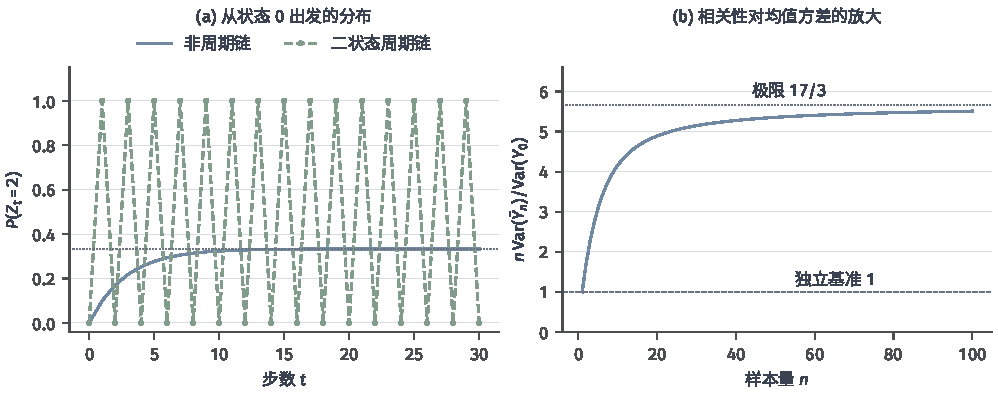
\includegraphics[width=\linewidth]{figures/00-shared/mathematical-preliminaries-lower/01-random-variables-distributions-and-causality/matplotlib/stochastic-mixing-variance/figure.pdf}
  \caption{两状态链的解析式教学图。左图蓝线使用例~\ref{ex:stoch-two-state-chain}的转移矩阵，从\(Z_0=0\)出发绘制\(\mathbb P(Z_t=2)=(1-0.7^t)/3\)；绿线使用确定交替的转移矩阵。右图使用平稳初态和\(\rho_k=0.7^k\)，绘制\(1+2\sum_{k=1}^{n-1}(1-k/n)\rho_k\)，其极限为\(17/3\)，独立观测基准为\(1\)。}
  \label{fig:stochastic-mixing-variance}
\end{figure*}

\subsection{随机路径的收敛}
\label{sec:rv-path-convergence}
前面讨论同一个过程是否有连续版本；现在比较的是一列过程及其极限。路径极限
把整条函数当成随机对象，必须先规定函数之间怎样接近。对实值连续路径，
\(C([0,T])\)取一致距离
\(\|x-y\|_\infty=\sup_{t\leq T}|x(t)-y(t)|\)，是Polish空间。
对右连续且有左极限的路径，使用\(D([0,T])\)及Skorokhod \(J_1\)拓扑：
若存在严格递增的连续双射\(\lambda_n:[0,T]\to[0,T]\)，使
\[
\|\lambda_n-\operatorname{id}\|_\infty\to0,\qquad
\|x_n\circ\lambda_n-x\|_\infty\to0,
\]
就有\(x_n\to x\)于该拓扑。它允许跳跃时刻略微错开，再对齐比较；相应拓扑可由完备可分度量刻画。若极限连续，\(J_1\)收敛等价于一致收敛。

图~\ref{fig:probability-skorokhod-jump-alignment}用只有一次跳跃的路径说明时间校正的作用。令\(x(t)=\mathbb I\{t\geq1/2\}\)、\(x_n(t)=\mathbb I\{t\geq\tau_n\}\)，其中\(\tau_n=1/2+0.1/n\)。在两次跳跃之间，一条路径已经取\(1\)，另一条仍取\(0\)，所以普通一致误差始终等于\(1\)。取连接\((0,0)\)、\((1/2,\tau_n)\)、\((1,1)\)的分段线性\(\lambda_n\)，它是区间上的严格递增连续双射，并把目标跳跃时刻送到\(x_n\)的跳跃时刻。于是\(t<1/2\)时\(\lambda_n(t)<\tau_n\)，\(t\geq1/2\)时\(\lambda_n(t)\geq\tau_n\)，逐点得到\(x_n\circ\lambda_n=x\)，从而
\[
 \|x_n-x\|_\infty=1,\qquad
 \|\lambda_n-\operatorname{id}\|_\infty=0.1/n\longrightarrow0,\qquad
 \|x_n\circ\lambda_n-x\|_\infty=0.
\]
这个例子正好满足\(J_1\)的两个条件，却不满足普通一致收敛；极限路径的跳跃使这两种比较方式产生区别。

\begin{figure*}[htbp]
  \centering
  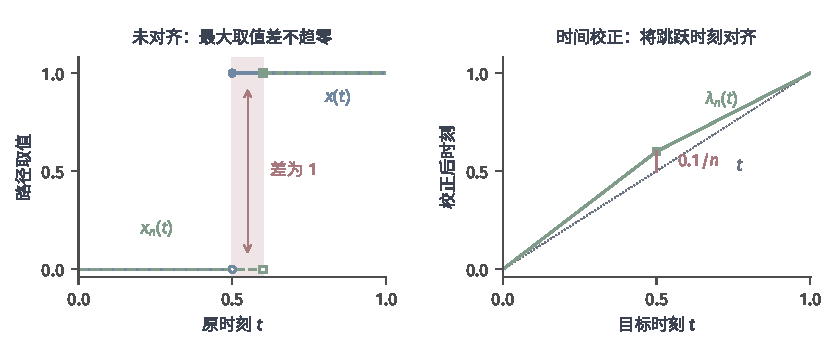
\includegraphics[width=140mm]{figures/00-shared/mathematical-preliminaries-lower/01-random-variables-distributions-and-causality/matplotlib/probability-skorokhod-jump-alignment/figure.pdf}
  \caption{跳跃时刻对齐与\(J_1\)收敛（解析式教学图，展示\(n=1\)）。左图蓝实线的跳跃位于\(1/2\)，绿虚线的跳跃位于\(\tau_n=1/2+0.1/n\)；浅红时间带内二者取值相差\(1\)，实心与空心点区分端点是否取到。右图分段线性时间校正通过\((1/2,\tau_n)\)，相对恒等映射的最大偏差为\(0.1/n\)；经\(x_n\circ\lambda_n\)复合后，两条路径完全重合。}
  \label{fig:probability-skorokhod-jump-alignment}
\end{figure*}

有限维收敛仍不够。取确定连续函数
\[
x_n(t)=\max\{1-n^2|t-1/n|,0\},\qquad 0\leq t\leq1,\ n\geq2.
\]
每个固定时刻最终避开窄尖峰，所以任意有限维向量趋零；但
\(\|x_n\|_\infty=1\)，不可能在\(C([0,1])\)中趋零。
越来越窄的尖峰没有被有限个截面发现，却阻止了路径规律的紧性。

\begin{theorem}[连续路径的紧性与极限识别]
\label{thm:rv-continuous-path-tightness}
设\(X_n\)是\(C([0,T])\)值随机对象。令
\[
w(x,\delta)=\sup_{\substack{s,t\in[0,T]\\|t-s|\leq\delta}}|x(t)-x(s)|.
\]
若\((X_n(0))\)的分布一致紧，且对每个\(\varepsilon>0\)，
\[
\lim_{\delta\downarrow0}\sup_n
\mathbb P\{w(X_n,\delta)>\varepsilon\}=0,
\]
则路径分布一致紧。若其有限维分布还收敛到某个连续过程\(X\)的有限维分布，则
\(X_n\Rightarrow X\)于\(C([0,T])\)。
\end{theorem}
这里用到Arzelà--Ascoli定理的确定性形式：紧区间上一族连续函数若统一有界且等度连续，其一致范数闭包就是紧集。等度连续指对每个误差阈值，都能选择同一个时间间隔，同时控制族内全部函数的短时变化；每个函数各自连续还不够。Arzelà--Ascoli定理的证明见实分析教材\scite{math-folland1999real}；概率路径紧性的论证接着把这些紧集用于控制路径分布。

为把概率条件对应到这两项要求，固定\(0<\epsilon<1\)。由初值一致紧选\(M<\infty\)，使
\(\sup_n\mathbb P(|X_n(0)|>M)\leq\epsilon/2\)。
再取\(\eta_k=2^{-k}\)，逐个选取递减的\(\delta_k\downarrow0\)，使
\[
 \sup_n\mathbb P\{w(X_n,\delta_k)>\eta_k\}
 \leq\epsilon\,2^{-k-1},\qquad k\geq1.
\]
联合界说明每条\(X_n\)以至少\(1-\epsilon\)的概率同时满足初值界和全部尺度的振荡界。
满足这些限制的确定性路径族等度连续；把\([0,T]\)分成有限个长度不超过\(\delta_1\)的小段，还得到统一幅度界
\(M+\lceil T/\delta_1\rceil\eta_1\)。
因此其闭包是承载至少\(1-\epsilon\)概率的紧集，得到所需路径分布的一致紧性。

Prokhorov定理给出子列极限，坐标评价在\(C\)中连续，因此有限维规律识别每个子列极限。连续路径的Borel规律由稠密时刻坐标决定，故所有子列指向同一个极限。
若存在\(p>0\)、\(\beta>0\)及有限常数\(C\)，对全部\(n,s,t\)统一满足矩界
\(\mathbb E|X_n(t)-X_n(s)|^p\leq C|t-s|^{1+\beta}\)，且初值一致紧，则是上述模连续性条件的一项常用充分条件。

跳跃路径不能使用同一个连续模量：一个合法跳跃已使其无法趋零。对
\(D\)空间须另证\(J_1\)紧性，再在极限几乎必然连续的时刻核对有限维收敛。例如可用有界时间内的紧包含条件及停时短增量条件建立紧性；这些是额外假设，不由单时刻收敛自动成立。

缩放随机游走给出重要入口。若\(\xi_i\)独立同分布、均值零、方差一，
令\(S_k=\sum_{i=1}^k\xi_i\)，在网格\(k/n\)上取\(S_k/\sqrt n\)并作线性插值。
Donsker定理说明这些随机折线在\(C([0,T])\)中弱收敛到标准Brownian运动\scite{math-kallenberg2021probability}。
阶梯插值相应在\(D\)的\(J_1\)拓扑收敛。这里同时需要有限维极限与路径紧性，不能只把单时刻中心极限定理改写成带\(t\)的公式；Brownian的完整定义见第~\ref{sec:dynamical-brownian-motion}节，随机折线的构造则说明该路径规律怎样作为离散累计量的极限出现。


\section{本章小结}
\label{sec:stochastic-processes-and-approximation-summary}
\label{sec:random-sequences-and-processes-summary}

相同的单时刻分布可以对应不同的序列和路径。有限维联合规律保留坐标之间的联系，历史条件说明下一步允许依赖什么，路径条件则约束一次实现的连续性与跳跃。独立性、交换性、Markov性、鞅关系与平稳性各自限制不同的对象，不能由其中一种条件替代其余条件。

累计误差需要同时说明观测预算与结论的概率含义。固定时刻的集中不能自动覆盖看过记录后选出的时刻或候选；大数定律和中心极限定理也不直接给出当前预算下的误差概率。相关状态的时间平均可能收敛，而每一步的边缘规律仍周期振荡；路径极限又要求控制整族短时变化，超出逐个时刻极限所能保证的范围。

采样积分把这些结论用于给定规律下的计算。换测度保证平均目标可以改写，方差缩减还需额外的矩、辅助均值或条件积分信息；权重可计算与方差有限也须分别核对。随机比值和非线性变换的长期误差依赖概率阶、连续映射及局部展开，方差近似稳定并不免除反变换偏差。下一章将把给定规律改为未知观测模型，研究有限记录能够支持哪些统计结论。

